\documentclass[11pt]{report}

\usepackage[british]{babel}
\usepackage{lipsum} % pack�age to generate filler text Lorem Ip�sum dummy text 
\usepackage[margin=25.4mm,includefoot]{geometry} % geometry package to define margins. Possibility to make left margin larger for binding the document.

\usepackage[hidelinks]{hyperref}  % Allows for clickable reference
\hypersetup{colorlinks = true, linkcolor=blue, citecolor = {blue}, urlcolor=blue,}
\usepackage{enumitem}
%\usepackage[absolute]{textpos}
\usepackage[overlay,absolute]{textpos}

% Graphics preamble
\newcommand\scalemath[2]{\scalebox{#1}{\mbox{\ensuremath{\displaystyle #2}}}}
\usepackage{graphicx} % Alows you to import images
\graphicspath{{figures/}}
\usepackage{caption}
\usepackage{subcaption}
\usepackage{float} % Allows for control of float positions
\usepackage[table,xcdraw]{xcolor}
\usepackage{rotating}
\usepackage{pdflscape}

\usepackage{booktabs}

% Header and Footer Stuff
\usepackage{fancyhdr}   % package for extensive control of page headers and footers
\pagestyle{fancy}
\fancyhead{}
\fancyfoot[C]{\thepage}% Page numbering for center footer
\renewcommand{\headrulewidth}{0pt}    % Removes beautiful line in header
\renewcommand{\footrulewidth}{1pt}
\usepackage[bottom]{footmisc}  % keeps footnotes at bottom of page
\usepackage{multirow}
\setcounter{secnumdepth}{3}
\setcounter{tocdepth}{3}

% Bibliography preamble
\usepackage[round]{natbib}

% Math preamble
\usepackage[short]{optidef} % Why is this package not papering?
\usepackage{amsmath,amssymb,amsthm,mathtools,bm,etoolbox, cases, commath}
\newtheorem{myax}{Axiom}[chapter]
\newtheorem{mydef}{Definition}[chapter]
\newtheorem{myth}{Theorem}[chapter]
\usepackage{algorithm}
\usepackage {algpseudocode}
\usepackage{cases}
\usepackage{bbm}

% Research question preamble
\newtheorem{question}{Question} 
\newcounter{subq} 
\newcommand{\subq}{ 
  \setcounter{subq}{0} 
  \renewcommand\thequestion{\protect\stepcounter{subq}% 
  \arabic{question}\alph{subq}\protect\addtocounter{question}{-1}} 
} 

\newcommand{\normquestion}{ 
  \renewcommand\thequestion{\arabic{question}} 
  \stepcounter{question} 
} 


\begin{document}

\begin{titlepage}
%\begin{center}
\iffalse

\includegraphics[height=2cm]{tue-logo-high}\\

\large
Department of Industrial Engineering and Innovation Sciences  \\
Operations, Planning, Accounting and Control Research Group
\fi
\hfill Eindhoven, July 2018

\vspace*{10cm}

%\setlength{\TPHorizModule}{1mm}
%\setlength{\TPVertModule}{\TPHorizModule}
% Set the Paragraph Indent to zero, so the first line is not Indented
% Back-up the current value so it can be put back at the end of the title page
\newlength{\backupparindent}
\setlength{\backupparindent}{\parindent}
\setlength{\parindent}{0mm}			
\iffalse
\begin{textblock}{165}(45,90)
    \vspace*{1mm}
    \huge
    \textbf{Conditional Correlation Modeling using Multivariate GARCH and Machine Learning \\}
    \Large
    \vspace*{10mm}
    in partial fulfillment of the requirements for the degree of \\
     \vspace*{5mm}
\textbf{Master of Science in \\ Operations Management and Logistics}\\
    \vspace*{10mm}
    \Large
    P.G. Melkert \\
    Student identity number 0893899	
\end{textblock}
\fi
%%%%%%%%%% TUE SPECIFICATION TITLE PAGE %%%%%%%%%%%%
% Textblock width 90 mm, pos x,y (60, 73)
\begin{textblock*}{90mm}(60mm,73mm)
    \vspace*{1mm}
    \Large
    \textbf{Conditional Correlation Modeling \\ using Machine Learning and \\ Multivariate GARCH }
    \vspace*{1mm}    
    
    \normalsize   
    by \\
    Paul G. Melkert \\
\end{textblock*}
\vspace*{15mm}

\begin{center}
Student identity number 0893899	 \\
     \vspace*{15mm}
    in partial fulfilment of the requirements for the degree of \\
     \vspace*{5mm}
\textbf{Master of Science \\ in Operations Management and Logistics}\\
    \vspace*{5mm}



\vfill



\vfill
Draft
\vfill

\setlength{\parindent}{\backupparindent}
\end{center}

\mbox{}
\vfill
\noindent
Supervisors:\\
Dr. A. Chockalingam, Eindhoven University of Technology, OPAC \\
Dr. R.J. de Almeida e Santos Nogueira, Maastricht University, Quantitative Economics


\clearpage

\noindent
TUE. School of Industrial Engineering. \\
\noindent
Series Master Theses Operations Management and Logistics
\vfill
\noindent
Subject headings: Conditional Correlation; Semiparametric Multivariate GARCH; Nearest Neighbor; Random Forest; Conditional Covariance.  
\vspace{0.5\textheight}

\pagenumbering{gobble}
\end{titlepage} 


\pagenumbering{roman}

\section*{Abstract}    % Asterisk is to remove header numbering (and toc)
\addcontentsline{toc}{section}{\numberline{}Abstract}  % Gets summary in toc
"In this paper we develop a new semiparametric model for conditional correlations, which combines parametric univariate Generalized Auto Regressive Conditional Heteroskedasticity specifications for the individual conditional volatilities with nonparametric machine learning regressors nearest neighbor and random forest for the conditional correlations. This approach not only avoids the rapid increase in parameters as the number of assets becomes large, which typically happens in conventional multivariate conditional volatility models, but also the rigid structure imposed by more parsimonious models, such as the dynamic conditional correlation model. An empirical application to the 30 constituents included in the Dow Jones Industrial Average index demonstrates that the model is able to capture interesting conditional properties in correlations and that it is competitive with standard parametric models in terms of estimating a common risk measure such as Value-at-Risk."

\iffalse
ref:Hafner2006: "In this paper we develop a new semiparametric model for conditional correlations, which combines parametric univariate Generalized Auto Regressive Conditional Heteroskedasticity specifications for the individual conditional volatilities with nonparametric kernel regression for the conditional correlations. This approach not only avoids the proliferation of parameters as the number of assets becomes large, which typically happens in conventional multivariate conditional volatility models, but also the rigid structure imposed by more parsimonious models, such as the dynamic conditional correlation model. An empirical application to the 30 Dow Jones stocks demonstrates that the model is able to capture interesting asymmetries in correlations and that it is competitive with standard parametric models in terms of constructing minimum variance portfolios and minimum tracking error portfolios."
\fi

\iffalse
"In this paper, we propose the first KNN and RF for modeling conditional correlations of financial market returns and to improve moving window correlation estimates. The methods capture time varying correlation and conditional volatility without an underlying restricted statistical model for the correlations. " \\


\noindent
In this paper we propose an estimator of the conditional covariance matrix in a quantitive finance setting. Based on the estimation of conditional correlations using machine learning algorithms, this methodology provides an efficient estimator from a semi parametric point of view. \\



\noindent
"In this paper we show that (parsimonious) machine learning algorithms can be used to model unobserved conditional pairwise correlations between a set of financial market returns, where the obtained pairwise
correlations lead to a multivariate volatility model with conditional properties. The proposed methods avoid strong distributional assumptions on the correlation process and uses the conventional approximation of conditional correlation, namely sample correlations from moving windows, as covariate and response variables. The covariate space of the machine learning algorithms is kept parsimonious through defining the minimum and maximum past log return and past correlation as indicators of the overall correlation pattern in the market". We carried out numerical experiments based on financial market returns that show the applicability of the proposed machine learning estimation methods in specific practical situations. "A comparison was carried out with respect to a parsimonious and industry standard benchmark for conditionally heteroscedastic class of models, namely, Dynamic Conditional Correlation." \\

\noindent
Stochastic correlation forecasts are evaluated within the context of risk management. "We use the model to estimate the conditional covariance of up to 30 assets using Dow Jones Industrial Average stocks, and conduct specification tests of the estimator using an industry standard benchmark for volatility models (Dynamic Conditional Correlation model). This new estimator demonstrates very strong performance especially considering ease of implementation of the estimator." \\


"More accurate models of risk, as the ones proposed in this paper, can lead to better assessment and understanding of held portfolios and market exposure. The performance of VaR models is evaluated by using an unconditional coverage test (Kupiec test) and an independence test (Christoffersen Markov test)". It is (hopefully) found that the DCC-GARCH model is sometimes rejected, while the machine learning algorithms of VaR are never/ less frequently  ejected.
\fi




         


\cleardoublepage 

\section*{Acknowledgments}    % Asterisk is to remove header numbering (and toc)
\addcontentsline{toc}{section}{\numberline{}Acknowledgments}  % Gets summary in toc
This paper would not have come to its successful conclusion without the support of my university advisors. Therefore, I would like to sincerely thank Dr. Arun Chockalingam and Dr. Rui Almeida for their help, guidance and freedom that I was granted throughout these months. I am grateful to them for their interest in this work and for reserving the time to asses it.

\cleardoublepage



% Table of Contents stuff
\tableofcontents
\thispagestyle{empty}   % removes page numbering and footer from content page 
\cleardoublepage          % clears the rest of the page

% List of figures, list of tables
\listoffigures
\addcontentsline{toc}{section}{\numberline{}List of Figures}
\cleardoublepage

\listoftables
\addcontentsline{toc}{section}{\numberline{}List of Tables}
\cleardoublepage

\vspace*{\fill} 
\begin{quote} 
\centering 
Essentially, all models are wrong, but some are useful. - \cite{ref:Box1987} 
\end{quote}
\vspace*{\fill}


\cleardoublepage 


% Main body stuff
\pagenumbering{arabic}
\setcounter{page}{1}     % set Introduction as page 1



%NEW CHAPTER 
\chapter{Introduction}\label{sec:intro} 
Correlations are essential inputs for many of the core modeling problems in financial econometrics. Hedges, for example, call for estimates of correlation between the asset returns comprising the hedge. When correlations and volatilities change with the revealing of new information, a proper hedge should reflect the most recent information by adjustment of the hedge ratio. Analogously, derivatives such as rainbow options that comprise two or more underlying assets have prices that are dependent on the correlation between the underlying asset returns. In fact, any pricing formula is premised on estimates of future correlations and volatilities. \\   

\iffalse
"Correlations are critical inputs for many of the common tasks of � financial management. Hedges require estimates of the correlation between the returns of the assets in the hedge. If the correlations and volatilities are changing, then the hedge ratio should be adjusted to account for the most recent information. Similarly, structured products such as rainbow options that are designed with more than one underlying asset have prices that are sensitive to the correlation between the underlying returns. A forecast of future correlations and volatilities is the basis of any pricing formula. 
\fi

\noindent
Correlations are also essential inputs for the tasks of asset allocation and risk management. In this context, however, large systems of correlations are generally required. Portfolio optimization methods used for finding an optimal portfolio given a set of constraints require an estimate of the variance-covariance matrix of future returns. Analogously, calculation of common risk measures such as the standard deviation or Value-at-Risk require estimates of the variance-covariance matrix. These tasks involve estimation of high dimensional variance-covariance matrices, potentially comprising thousands of assets.   \\  

\iffalse
Asset allocation and risk assessment also rely on correlations; however, in this case a large number of correlations is often required. Construction of an optimal portfolio with a set of constraints requires a forecast of the covariance matrix of the returns. Similarly, the calculation of the standard deviation of today's portfolio requires a covariance matrix of all the assets in the portfolio. These functions entail estimation and forecasting of large covariance matrices, potentially with thousands of assets. \\
\fi

\noindent
Modeling of correlations between financial variables has been the object of academic research for decades. Basic methods such as sample correlations from moving windows and exponential smoothing are commonly used. More involved methods such as univariate generalized autoregressive conditional heteroskedasticity (GARCH) models have been proven rather adequate to capture certain statistical properties of conditional volatility such as volatility clustering and conditional dynamics. In a parametric framework, a variety of multivariate GARCH models has been developed to model the  conditional covariance and correlations. For some interesting specifications of multivariate GARCH models, see the work of \cite{ref:Bollerslev1988}, \cite{ref:Engle1995}, \cite{ref:Engle1990}, \cite{ref:Ding2001}, \cite{ref:Alexander1997}, \cite{ref:Weide2002}, \cite{ref:Bollerslev1990}, \cite{ref:Engle2001}, \cite{ref:Engle2002}, and \cite{ref:Lanne2007}. A number of studies has provided empirical evidence on the use of multivariate GARCH models for modeling conditional covariance in asset allocation and risk measurement. For examples on high dimensional problems, examine the paper of \cite{ref:Engle2008} and \cite{ref:Laurent2012}. Parametric multivariate GARCH models, however, impose arbitrary assumptions on the distribution and functional form of the conditional covariance matrix. Misspecification of either potentially results in inefficient or inconsistent models.    \\

\iffalse
The quest for reliable estimates of correlations between �financial variables has been the motivation for countless academic articles and practitioner conferences and much Wall Street research. Simple methods such as rolling historical correlations and exponential smoothing are widely used. More complex methods, such as varieties of multivariate generalized autoregressive conditional heteroskedasticity (GARCH) or stochastic volatility, have been extensively investigated in the econometric literature and are used by a few sophisticated practitioners. To see some interesting applications, examine the paper of Bollerslev, Engle, and Wooldridge (1988), Bollerslev (1990), Kroner and Claessens (1991), Engle and Mezrich (1996), Engle, Ng, and Rothschild (1990), Bollerslev, Chou, and Kroner (1992), Bollerslev, Engle, and Nelson (1994), and Ding and Engle (2001). In very few of these articles are more than � five assets considered, despite the apparent need for bigger correlation matrices. In most cases, the number of parameters in large models is too big for easy optimization. \\
\fi

\noindent
An alternative to the parametric estimation of the conditional covariance matrix is provided by non- and semiparametric models. In contrast to parametric estimation, nonparametric models do not impose (potentially misspecified) arbitrary assumptions on the distribution or functional form of the object being estimated. Semiparametric models comprise methods that contain both fully parametric components and fully nonparametric components, and may prove to be appropriate in cases nonparametric models are not;  for example, in case of implications of the curse of dimensionality or lack of knowledge on the distribution of errors \citep{ref:Li2006}. Although semiparametric models may inherit desirable properties of a nonparametric model in that they are robust against misspecification on distributional assumption and functional form, the reliance on parametric assumptions does not exclude semiparametric models from inconsistency due to misspecification. Although there are numerous papers on nonparametric models for the conditional variance, there is a limited number of papers on fully nonparametric multivariate volatility models. For some interesting applications, examine the paper of \cite{ref:Long2005}, and \textbf{Add some more recent work}. \\

\noindent
Existing semiparametric multivariate volatility approaches may be based on the premise of a finite-dimensional parameter functional form for the conditional covariance matrix while the error distribution is estimated non- or semiparametrically, or on the premise of a finite-dimensional parameter functional form for the conditional variance while the conditional correlations are estimated nonparametrically. For some applications where the error distribution is estimated nonparametrically using kernel functions, examine the work of \cite{ref:Long2005}, \cite{ref:Hafner2007}, \cite{ref:Long2011} \iffalse \footnote{A semiparametric conditional covariance model is proposed that combines parametric and nonparametric estimators of the conditional covariance matrix in a multiplicative way.} \fi, and \textbf{Add some more recent work}. For some interesting Bayesian-based semiparametric multivariate GARCH models, examine the paper of \cite{ref:Jensen2013}\iffalse \footnote{A Bayesian nonparametric modeling approach is proposed for the error distribution in multivariate GARCH models.}\fi and \cite{ref:Virbickait2016}. For some interesting (conditional) copula-based semiparametric multivariate GARCH models\iffalse \footnote{This class of models considers the conditional variance of each marginal time series to be specified parametrically through univariate GARCH-type models where non- or semiparametric estimation of the univariate marginal distributions is followed by a parametric specification of the copula function, which specifies the dependence structure between the marginal series.\fi \iffalse the multivariate distribution of the standardized innovation are specified semiparametrically as a parametric copula evaluated at nonparametric marginals.} \fi, examine the work of  \cite{ref:Chen2006}, \cite{ref:Patton2006}, \cite{ref:Jondeau2006}, \cite{ref:Ausin2010}, and \textbf{Add some more recent work}. Finally, for some interesting applications belonging to the second category, examine the work of \cite{ref:Hafner2006}\iffalse\footnote{A nonparametric estimator is considered for the correlation function where a Nadaraya-Watson kernel regression is applied to each conditional correlation individually.}, and \textbf{Add some more recent work}\fi. \\     


\noindent
The aim of this paper is to develop a new semiparametric model for the conditional covariance matrix that is flexible and remains easy to estimate in high dimensional systems. The model is semiparametric in that it combines parametric univariate Generalized Auto Regressive Conditional Heteroskedasticity specifications for the individual conditional volatilities with nonparametric machine learning regressors for the conditional correlations. The choice for machine learning regressors is motivated by the fact that machine learning has been responsible for significant advances in a variety of research areas in the past decade; self-driving cars, speech and facial recognition, effective web search, and medical diagnostic procedures. However, the approach of using machine learning for the estimation of conditional correlation between financial variables has not been extensively investigated in scientific literature. In fact, there is a limited number of papers on this type of machine learning applications. For initial applications, see the papers of \cite{ref:Basturk2016_1} and \cite{ref:Basturk2016}, where a Probabilistic Fuzzy System is used to model the unobserved conditional correlation between financial returns in a bivariate and multivariate setting, respectively. \textbf{Add some more recent work if found.}    \\

\noindent
In this paper, two nonparametric learning algorithms, nearest neighbor and random forest, are considered for point estimating conditional correlations directly and independently of conditional volatilities. These learning methods have a clear advantage over multivariate GARCH models in that any imposition of arbitrary (potentially misspecified) assumptions on the distribution and functional form of the conditional correlation matrix is avoided; the conditional correlations are only assumed to depend on lagged sample correlations obtained using moving window estimation. Moreover, due to a parsimonious model specification, our semiparametric model for the conditional covariance matrix does not suffer from the curse of dimensionality to the same extent as early-stage multivariate GARCH models and many fully nonparametric models. Lack of imposed structure, however, does not guarantee that the obtained conditional correlation matrix is positive definite, which is verified with obtained correlation coefficients.        \\

\noindent
In this paper, using simulation, the performance of conditional correlations estimated by proposed learning methods and conventional moving windows is compared in terms of a statistical loss function, the mean squared error. In an empirical application, the proposed semiparametric multivariate volatility model is applied to the 30 constituents included in the Dow Jones Industrial Average index. Performance is verified in terms of an economic loss function, the Value-at-Risk, as the true conditional covariance matrix is unobservable. It is demonstrated that our semiparametric model is able to capture interesting conditional properties in correlations and that it shows competitive performance with a multivariate parametric counterpart, the Dynamic Conditional Correlation model of \cite{ref:Engle2002}.  \\

\noindent
The remainder of the paper is organized as follows. Chapter 2 gives an overview of the methodological underpinnings of multivariate volatility modeling and machine learning. Chapter 3 describes a simulation experiment and out-of-sample results are presented. Section 4 provides an empirical application to the 30 constituents included in the Dow Jones Industrial Average index to test the out-of-sample performance of the proposed model. Finally, conclusions and directions for future research are provided in Chapter 5. \\
 


\iffalse
\noindent
"In this paper, we put forward a new semiparametric model for the conditional covariance matrix that is flexible yet easy to estimate even in high dimensions. The model is semiparametric, in the sense that the conditional variances are described parametrically, for example, using standard univariate GARCH-type models, while the conditional correlations are estimated using nonparametric techniques." The conditional correlations are assumed to depend on past approximations of correlation. "For example, we model the correlations between the 30 individual stocks included in the Dow Jones Industrial Average (DJIA) index, and allow these to depend on past approximations of correlation. These variables are motivated by" the wish of keeping the model parsimonious in nature.  \\


\noindent
\textit{nearest neighbor and random forests are considered as non-parametric learning algorithms since the number of parameters grows with the size of the training set.} \\

\noindent
\textbf{Speak of curse of dimensionality and how knn and rf deal with this}\textit{knn with exhaustive search does not suffer from curse of dimensionality. RF has also a reduced risk of overfitting compared to other machine learning methods, which is crucial for situations where the dataset has many more features than samples. These situations suffer from the ?curse of dimensionality,? and RF overcomes this by building independent decision trees each trained on a sub-sampled range of the dataset with the global decision based on all ensemble of trees. Random Forests can handle high dimensional data by building large number of trees using only a subset of features. This combined with the fact that the random selection of features for a split seeks to minimize the correlation between the trees in the ensemble, certainly helps in building an ensemble classifier with high generalization accuracy for high dimensional data problems.} \\

\fi



\iffalse
\noindent
"First, popular parametric models are rarely, if ever, correctly specified The ?horse race? is therefore between misspecified and therefore inconsistent parametric models and relatively inefficient but
consistent nonparametric models." \\
\fi




\section{Problem Statement}
The following properties of correlation make the modeling and forecasting of (systems of) correlation(s) inherently complex:

\begin{enumerate}
	\item Correlation is not directly observable.
	\item Correlation between financial variables is time-varying, that is, conditional on information available at time $t$.
	\item Curse of dimensionality: the number of pairwise correlation grows $O(k^2)$ in the number of assets $k$. 
	\item Conditional correlation matrix requires to satisfy positive definiteness.
	\item Any imposition of arbitrary assumptions on the distribution and functional form of the conditional correlation matrix is highly questionable.  
\end{enumerate}

\noindent
This paper will address the last issue by defining the estimation of conditional correlation between financial returns as a supervised learning problem. However, in defining the task of estimating conditional correlations as a supervised learning problem, the unobservability of conditional correlation, the time-varying property, the curse of dimensionality, and the positive definiteness requirement are considered. Machine learning provides an approach that enables us to extract correlation information without the imposition of arbitrary assumptions on the distribution and functional form of the conditional correlation matrix, which is crucial in applications where any kind of distributional assumption is highly questionable. Understanding and quantification of conditional correlation between financial returns is an example of such an application \citep{ref:Christoffersen1998}.   \\


\section{Research Objectives}
The aim of this paper is to develop a new semiparametric model for the conditional covariance matrix that is flexible and remains easy to estimate in high dimensional systems. The model is semiparametric in that it combines parametric univariate Generalized Auto Regressive Conditional Heteroskedasticity specifications for the individual conditional volatilities with nonparametric machine learning regressors nearest neighbor and random forest for the conditional correlations. We are interested in the performance of proposed semiparametric multivariate volatility model when evaluated against conventional methods. As such, we can formulate the following research objectives:  \\

\begin{enumerate}
	\item Formulate the task of estimating conditional correlation between financial returns as a supervised learning problem.
	\item Given the supervised learning problem formulation, design and implement a Nearest Neighbor and Random Forest estimator with support for high dimensional regression output problems.  
	\item Evaluate the machine learning estimators against conventional methods for estimating conditional correlation.  
	\item Evaluate the proposed semiparametric model for the conditional covariance matrix against conventional methods for estimating multivariate volatility.  
\end{enumerate}

\iffalse
\noindent
First, through implementation of a simulation study, we aim to verify whether proposed learning algorithms have any capability in estimating conditional correlation between financial returns in a bivariate setting; two asset return paths with a predefined correlation structure. More precisely, we seek to verify whether nearest neighbor and random forest learning algorithms improve over conventional moving window approximation of conditional correlation. The controlled setting of a simulation study allows us to observe the effect of different foundational model properties (parameterizations) on the generalization error. By defining the generalization error as the mean squared error loss, we will be able to observe the effect of incorporating approximation error due to defining the set of covariates and response variable using moving window estimates of correlation. \\

\noindent
Next, we extend the empirical evaluation of conditional correlation modeling to a multivariate setting. The focus will be on systems of correlations rather than individual correlations. The proposed semiparametric multivariate volatility model is applied to the 30 constituents included in the Dow Jones Industrial Average index. In this context, our semiparametric multivariate model is kept parsimonious in parameterization to overcome the difficulty of curse of dimensionality. The proposed model is very flexible but the lack of imposed structure does not guarantee the resulting conditional covariance matrix to be positive definite such that this must be verified with obtained parameters. Performance is verified in terms of an economic loss function, the Value-at-Risk, as the true conditional covariance matrix is unobservable. The Value-at-Risk forecasts are statistically compared on two properties: unconditional coverage property and independence property. Evaluation is done against a multivariate parametric counterpart, the Dynamic Conditional Correlation model of \cite{ref:Engle2002}.     
\fi
 
\section{Outline and Contributions}
The main contribution of this paper is the development of a computational framework using nearest neighbor and random forest algorithms for the task of estimating conditional correlation between financial returns. We show that the integration of statistical models for capturing conditional volatility, such as univariate GARCH-type models, with proposed learning estimators provides a flexible, semiparametric way of formulating multivariate volatility models that avoid the imposition of (potentially misspecified) assumptions on the distribution and functional form of the conditional correlation matrix. \\ 

\noindent
Chapter \ref{ch:methodology} presents the methodological framework. The conceptual underpinnings of machine learning (algorithms) and multivariate volatility modeling are discussed. Moreover, an approach is presented to successfully address supervised learning in the context of estimating conditional correlation between financial returns. Given that correlation is not directly observable, construction of the set of covariates and response variables is done by approximation of true correlation using Pearson and Kendall sample correlations from moving windows. The result is a generic and parsimonious supervised learning problem formulation for the task of estimating conditional correlation, which should overcome the difficulty of the curse of dimensionality in high dimensional systems. Notably, the supervised learning problem formulation serves as basis for the first presentation of nearest neighbor and random forest estimators of conditional correlation between financial returns. \\

\noindent
Chapter \ref{ch:simulation_study} examines the accuracy of nearest neighbor and random forest estimators of correlation in a bivariate setting; two asset return paths with a predefined pairwise correlation structure. The controlled setting of a simulation study allows us to observe the effect of different foundational model properties on the generalization error, which is defined as the mean squared error loss in this chapter. On the premise of mean squared error loss, we are able to observe the effect of incorporation of approximation error due to defining the set of covariates and response variable using moving window estimates of correlation. It is shown that proposed learning estimators improve over conventional moving window approximation of conditional correlation through lower mean squared error and by decreasing the sensitivity of the results to the choice of window length in the moving window approximations of conditional correlation. Moreover, learning estimates with approximations of actual correlation as covariates and response variable follow the increases and decreases of actual correlation smoother, with tighter confidence intervals compared with Pearson and Kendall sample correlation estimates using moving windows. This is a more desirable result as it is not expected that correlation between assets changes that drastically on a daily basis. Additionally, both learning estimators exhibit expected behavior under different parameterizations given the theoretical analysis of mean squared error decomposition into squared bias and variance terms; an increase in the number of neighbors in the Nearest Neighbor and an increase in the number of decision trees in the Random Forest reduce the variance in both estimators. Finally, the conditional correlation matrix obtained under a variety of different parameterizations of Nearest Neighbor and Random Forest estimators satisfy the condition of positive definiteness. In summary, using simulation, initial evidence has been provided on the potential use of proposed learning estimators as estimators of conditional correlation between financial returns.  \\

\noindent
We then extend the empirical evaluation of correlation estimates using machine learning to a multivariate setting in Chapter \ref{chap:multivariate_analysis}. The focus of analysis is \textit{systems of correlations} in a quantitative financial risk management context rather than \textit{individual correlations}. The proposed semiparametric multivariate volatility model is applied to the 30 constituents included in the Dow Jones Industrial Average index and performance is verified in terms of an economic loss function, the Value-at-Risk. Evidence is provided that the model is able to capture interesting conditional properties in correlations and that it is competitive with a multivariate parametric counterpart, the Dynamic Conditional Correlation model of \cite{ref:Engle2002}. \textbf{Insert more detailled summary of empirical results: tranquil market conditions and volatile market conditions, unconditional coverage and independence test + main result.} \\

\noindent
Finally, Chapter \ref{ch:conclusion} contains a general conclusion of this paper as well as interesting directions for future research. \textbf{Insert direction of future research.}


\chapter{Methodology} \label{ch:methodology}
In this chapter, we will develop notation and basic approaches that will provide us with the foundational concepts used throughout this paper. Section \ref{sec:mvm} introduces the conceptual underpinnings of multivariate volatility modeling and introduces a class of parametric multivariate GARCH models that is premised on decomposition of the conditional variance-covariance matrix into conditional variances and conditional correlations. Moreover, the semiparametric character of our specification for the conditional covariance matrix will become apparent. Section \ref{sec:ml_supervised} introduces the concepts of machine learning and supervised learning. Theoretical background is given of the learning algorithms that lie at the core of nonparametric learning models k-nearest neighbor and random forest as well as the effect of foundational model properties on the generalization error. The latter is done through discussion of an important issue in machine learning, that is, the tradeoff between bias and variance. Finally, Section \ref{sec:cor_ml} presents an approach to successfully address supervised learning in the context of estimating conditional correlation between financial returns.

%%%%%%%%%%%%%%%%%%%%%%%%%%%%%%%%%%%%%%%%%%%%%%%%%%%%%%
%%%%%% 				     Multivariate Volatility Methodology 					%%%%%%%
%%%%%%%%%%%%%%%%%%%%%%%%%%%%%%%%%%%%%%%%%%%%%%%%%%%%%%
\section{Multivariate Volatility Modeling} \label{sec:mvm}
Asset allocation and risk management require the identification and quantification of the underlying co-movements in financial returns. This may be captured through specification of the conditional covariance matrix. Following the adequacy of univariate generalized autoregressive conditional heteroskedasticity (GARCH) models in capturing certain statistical properties of conditional volatility, a variety of multivariate GARCH models has been developed to specify the conditional covariance matrix. The different specifications of parametric multivariate GARCH models may be classified into three non-mutually exclusive groups as suggested in \cite{ref:Bauwens2006}; (1) direct extensions of the univariate GARCH model of \cite{ref:Bollerslev1986}; (2) factor models; (3) models of conditional variances and conditional correlations.    \\

\noindent
Models in the first group specify the conditional covariance matrix directly such as the Vector Error Correction (VEC) model of \cite{ref:Bollerslev1988} and BEKK model of \cite{ref:Engle1995}. These models allow for rich and flexible dynamics of the conditional covariance matrix due to their generality. However, even for low dimensions (3 or 4 assets), the heavily parameterized specifications of VEC and BEKK models become intractable due to the proliferation of parameters, even in restricted parameterizations such as diagonal VEC, diagonal and scalar BEKK. The second group comprises more parsimonious parameterizations of the conditional covariance matrix using factors. Examples are the factor GARCH model of \cite{ref:Engle1990}, the (generalized) orthogonal models of \cite{ref:Alexander1997}, \cite{ref:Weide2002}, and \cite{ref:Lanne2007}. For a more a comprehensive survey of these models, examine the work of \cite{ref:Bauwens2006}. Models in the third group are parsimonious in parameterization and premised on decomposition of the conditional covariance matrix into conditional variances and conditional correlations, which are then modeled separately. These models were first introduced through the Constant Conditional Correlation (CCC) model of \cite{ref:Bollerslev1990}, which assumed (unrealistically) conditional correlations to be constant over time. Generalization of the CCC model was proposed by \cite{ref:Engle2002} and \cite{ref:Tse2002}. These Dynamic Conditional Correlation models allow for both the conditional variance matrix and conditional correlation matrix to be time-varying. Moreover, the formulation of our semiparametric multivariate volatility model is premised on decomposition of the conditional covariance matrix into conditional variances and conditional correlations.   \\

\noindent
As such, in this paper, a mean-corrcted $k$-dimensional log return series, $r_t = (r_{1,t}, \dots, r_{k,t})'$, is considered such that

\begin{align} 
	r_t = H^{1/2}_t z_t \label{eq:returns_model}
\end{align}

\noindent
where $t \in \{1, \dots,T\}$ indicates the time unit, $z_t$ is a $k \times 1$ vector of i.i.d random variables with mean zero and unit variance, $H_t$ is a $k\times k$ positive definite matrix, and $H_t^{1/2}$  denotes the Cholesky decomposition of $H_t$. \\

\noindent
The conditional variance-covariances of returns $r_t$ are represented by the $k \times k$ matrix $\mathrm {Var}(r_t) = H^{1/2}_t H^{\prime 1/2}_t = H_t$, which by construction is not observable \citep{ref:Basturk2016}. A plethora of models has been proposed to model the conditional covariance matrix $H_t$ and we consider a reparameterization of $H_t$ that is a common approach for the identification of variances and correlation coefficients \citep{ref:Bauwens2006}, that is, 

\begin{align} \label{eq:covariance_decomposition} 
	H_{t}=D_{t}R_{t}D_{t} = 
		\begin{pmatrix} h_{1,1,t}^{1/2} &&0 \\ &\ddots \\ 0 &&h_{k,k,t}^{1/2} \end{pmatrix} 
		\begin{pmatrix} 1 &\rho_{1,2,t} &\cdots &\rho_{1,k, t} \\ \rho_{2,1,t} &1 & &\rho_{2,k, t} \\ \vdots &&\ddots &\vdots \\ \rho_{k, 1,t} &\rho_{k, 2,t} &\cdots &1 \end{pmatrix} 
		\begin{pmatrix} h_{1,1,t}^{1/2} &&0 \\ &\ddots \\ 0 &&h_{k,k,t}^{1/2} \end{pmatrix} 
\end{align}

\noindent
where $D_t$ is a diagonal matrix with conditional volatilities of each marginal series on its diagonal and matrix $R_t$ includes all pairwise correlations $\rho_{i,j,t}$, with $\rho_{i,j,t} = \rho_{j,i,t}$ (by definition). \\

\noindent
The semiparametric character of our specification for $H_t$ now becomes apparent: the diagonal elements of the matrix $D_t$ are modeled parametrically using, for example, standard univariate GARCH-type models, whereas the conditional correlation matrix $R_t$ is estimated in a nonparametric manner using nonparametric machine learning algorithms. Estimation of $D_t$  is independent of the estimation of pairwise correlations, $\rho_{i,j,t}$, in $R_t$. This is explained by the fact that $D_t$ defines the unconditional variance of each marginal series at time unit $t$, which is independent of correlations $R_t$  by definition \citep{ref:Basturk2016}. In order to ensure positive definiteness of the conditional covariance matrix $H_t$ at each time unit $t$, two necessary conditions need to be satisfied when specifying $R_t$, that is,  

\begin{enumerate}
	\item $R_t$ has to be positive definite with det($R_t) \geq$ 0. ($D_t$ is positive definite as all its diagonal elements are positive).
	\item The absolute value of all elements in the conditional correlation matrix $R_t$ need to be equal or less than one by definition. 
\end{enumerate}

\noindent
These necessary conditions for satisfying a positive definite matrix $R_t$ are generally obtained by the imposition of arbitrary assumptions on the the distribution and functional form of the conditional correlation matrix. In view of the fact that many nonparametric estimators of the covariance matrix are developed without explicit satisfaction of the positive definiteness condition during estimation, satisfaction of the conditions is in this paper verified with the obtained conditional correlation matrix. \\     

\noindent
We examine the parametric Dynamic Conditional Correlation model in further detail in the next section as the model will be evaluated against our semiparametric multivariate volatility model specification in Chapter \ref{chap:multivariate_analysis}.

\subsection{Dynamic Conditional Correlation Model} \label{sec:dcc}
The Dynamic Conditional Correlation (DCC) model \citep{ref:Engle2002} is a class of models that generalizes univariate GARCH models to the multivariate case. The DCC models capture the advantages of GARCH models and simplifies the computation of multivariate GARCH models such as VEC-GARCH and BEKK. Reparameterization of the covariance matrix lets the DCC model take advantage of the fact that the correlation matrix is generally easier to model than direct modeling of the covariance matrix. In the DCC models, time series of daily mean-corrected log returns on k assets $r_t=a_t$ is given by

\begin{align}
	r_t &= H_t^{\frac{1}{2}}z_t \\
	H_t &= D_t R_t D_t \\
	D_t &= diag(\sigma_{1,t}, \dots, \sigma_{k,t})
\end{align}

\noindent
where $H_t$ is the conditional covariance matrix and $R_t$ is the conditional correlation matrix. $D_t$ is a diagonal matrix with $\sigma_{1,t}, \dots, \sigma_{k,t}$ on the main diagonal, which can be estimated though univariate GARCH models. \\

\noindent
The idea behind DCC models is that multivariate volatility modeling can be divided into two estimation steps. Under assumption of conditional normality in the daily mean-corrected log returns $r_t$, the estimator gives rise to a log likelihood function. Without this assumption, an expected Quasi-Maximum Likelihood function is calculated \citep{ref:Engle2002}. As such, the first step is to estimate the conditional volatility series, $\sigma_{i,t}$, which is done under the assumption that marginal volatility series follow a univariate GARCH(1,1) process with Gaussian distributed errors, that is,

\begin{align}
	\sigma_{i,t}^2 &= \omega_i + \beta_i\sigma_{i,t-1}^2 + \alpha_i a_{i,t-1}^2 
\end{align}

\noindent
Then, in the second step, one can use the estimated conditional volatilities $\sigma_{i, t}$ to model the dynamics of the conditional correlation matrix $R_t$, that is,

\begin{align}
	R_t &= D_t^{-1} H_t D_t^{-1}
\end{align}     
 
\noindent
$R_t$, as noted by \cite{ref:Engle2002}, is the conditional volatility matrix of the marginally standardized residuals $\epsilon_t = (\epsilon_{1,t}, \epsilon_{2,t}, \dots, \epsilon_{k,t})$, where $\epsilon_{i,t} = a_{i,t} / \sigma_{i,t}$. In this paper, the multivariate standard normal and the multivariate standard Student t-distribution are considered for the conditional distribution $\epsilon_t$. \\

\noindent
In the DCC model of \cite{ref:Engle2002}, the conditional volatility matrix of the marginally standardized residuals, $\epsilon_t$, is modeled using a GARCH(1,1) structure and reparameterization of $R_t$ ensures necessary conditions for $R_t$ are satisfied, that is,

\begin{align}  
	Q_t &= (1-\theta_1-\theta_2) \bar{Q} + \theta_1 Q_{t-1} \theta_2 \epsilon_{t-1} \epsilon'_{t-1} \label{eq:DCC_Q} \\
	R_t &= diag(Q_t)^{-1} Q_t \ diag(Q_t)^{-1} \label{eq:DCC_R}
\end{align}

\noindent
In \eqref{eq:DCC_Q}, $Q_t$ is a positive definite matrix defining the structure of the correlation dynamics and $\bar{Q} = Cov(\epsilon_t \epsilon'_t) = \mathbb{E}[\epsilon_t \epsilon'_t]$ is the unconditional covariance matrix of the standardized residuals $\epsilon_t$\footnote{$\bar{Q}$ can be thought of as representing the long-run correlation structure and can be estimated by: $\bar{Q} = \frac{1}{T} \sum_{t=1}^T \epsilon_t \epsilon'_t$.}. In \eqref{eq:DCC_R}, $diag(Q)_t$ is a diagonal matrix with the square root of the diagonal elements of $Q_t$ at its diagonal. It is simply a normalization matrix to ensure the requirement that all elements in the conditional correlation matrix $R_t$ are bounded by -1 and 1. Parameters $\theta_1$, $\theta_2$ are non-negative real numbers satisfying $ 0 < \theta_1 + \theta_2 < 1$, which ensures $Q_t$ to satisfy the condition of a positive definiteness and consequently positive definiteness for $H_t$ under the condition that $D_t$ is also positive definite.\\ 

\noindent
Eq. \eqref{eq:DCC_Q} shows that the DCC model of \cite{ref:Engle2002} is very parsimonious as the dynamics of all conditional correlations are driven with only two parameters, $\theta_1$ and $\theta_2$, regardless of the number of assets $k$. This is a necessary condition to ensure positive definiteness of $R_t$ for all time $t$. Consequently, the DCC model is relatively efficient to estimate and remains tractable when $k$ grows large. However, the assumption that the evolution of all correlations follows the same dynamic structure, regardless of the assets involved, can be considered a weakness of the DCC model, especially in high dimensional systems comprising many asset return series. \\


\noindent
\textbf{The approximation used for one-step-ahead forecasts can be found in \cite{ref:Engle2001}}. \\



\subsection{Pearson Product-Moment Correlation Coefficient}
One method to model the pairwise correlation coefficients $\rho_{i,j,t}$ in the conditional correlation matrix $R_t$ is to use moving window correlation estimates. An advantage of this method is that it avoids strong distributional assumptions. Following \cite{ref:Basturk2016}, the sample correlation at a selected time window $\Delta t$ is used as a proxy for approximation of conditional correlations using Pearson's linear correlation coefficient, that is,

\begin{align}
	\hat{\mu}_{i,t} &= \frac{1}{\Delta t}\sum\nolimits_{t'=t-\Delta t+1}^t y_{i,t'}, \; \; \forall i \in \{1, \dots, k\} \label{eq:mw_mu} \\
	\hat{\sigma}_{i,t} &= \sqrt{\frac{1}{\Delta t}\sum\nolimits_{t'=t-\Delta t+1}^t (y_{i,t'}-\hat{\mu}_{i,t})^2}, \; \; \forall i \in \{1, \dots, k\}   \label{eq:mw_sigma} \\ 
	\hat{\sigma}_{i,j,t} &= \frac{1}{\Delta t} \sum\nolimits_{t'=t-\Delta t+1}^t (y_{i,t'}-\hat{\mu}_{i,t})(y_{j,t'}-\hat{\mu}_{j,t})  \; \; \forall i,j \in \{1, \dots, k\}   \label{eq:mw_cov} \\ 
	\hat{\rho}_{i,j,t} &= \frac{\hat{\sigma}_{i,j,t}}{\hat{\sigma}_{i,t} \hat{\sigma}_{j,t}} \label{eq:mw_rho} 
\end{align}   

\noindent
where $\hat{\mu}_{i,t}$ defines the mean estimate for random variable $i$ at time $t$, $\hat{\sigma}_{i,t}$ defines an estimate of the standard deviation for random variable $i$ at time $t$, and $\hat{\sigma}_{i,j,t}$ defines the covariance between random variables $i$ and $j$ at time $t$. Consequently, the Pearson product-moment correlation coefficient between random variables $i$ and $j$ at time $t$ is defined by $\hat{\rho}_{i,j,t}$. \\

\noindent
Note that the correlation coefficient is dimensionless and, by definition, takes values between $-1$ and $1$. If the correlation between two random variables is close to $|1|$, then that is an indication of a strong linear relationship between corresponding random variables. The nonparametric learning estimators proposed in this paper make use of the moving window correlation estimates in \eqref{eq:mw_mu}-\eqref{eq:mw_rho} to define the set of covariates and response variable.

\iffalse
Additionally, exponential weighting of correlation coefficients $\rho_{i,j,t}$ is included in the analysis. Introduction of exponential weighting, where present observations are given more weight than past measurements, potentially better characterizes the dynamics of evolving dependency structures between asset return paths. From an informational point of view it makes sense to assume recent events more valuable than remote ones. For the computation of weighted Pearson correlation coefficients a weight structure, $w_t \ge 0$, is introduced under the constraint $\sum_{t'=t-\Delta t+1}^t w_t = 1$, operating on sample means, variances and covariances according to \cite{ref:Pozzi2012}:

\begin{align}
	\hat{\mu}_{i,t}^w &= \sum_{t'=t-\Delta t+1}^t w_{t'} y_{i,t'}, \; \; \forall i \in \{1, \dots, k\} \label{eq:mw_mu_w} \\
	\hat{\sigma}_{i,t}^w &= \sqrt{\sum\nolimits_{t'=t-\Delta t+1}^t w_{t'} (y_{i,t'}-\hat{\mu}_{i,t}^w)^2}, \; \; \forall i \in \{1, \dots, k\}   \label{eq:mw_sigma_w} \\ 
	\hat{\sigma}_{i,j,t}^w &= \sum\nolimits_{t'=t-\Delta t+1}^t w_{t'} (y_{i,t'}-\hat{\mu}_{i,t}^w)(y_{j,t'}-\hat{\mu}_{j,t}^w)  \; \; \forall i,j \in \{1, \dots, k\}   \label{eq:mw_cov_w} \\   
	\hat{\rho}_{i,j,t}^w &= \frac{\hat{\sigma}_{i,j,t}^w}{\hat{\sigma}_{i,t}^w\hat{\sigma}_{j,t}^w} \label{eq:mw_rho_w} 
\end{align}  

\noindent
\cite{ref:Pozzi2012} use the exponential function as functional form for the weights, i.e. exponential smoothing. This is the kind of weighting also used in this paper such that the weights in \eqref{eq:mw_mu_w}-\eqref{eq:mw_rho_w} are defined as:

\begin{align} \label{eq:pearson_weights}
	w_{t'} = w_0 \; e^{\alpha(t'- \Delta t)}, \; \; \forall t' \in \{t-\Delta t+1, t-\Delta t, \cdots, t\} 
\end{align}   

\noindent
where $\alpha = \frac{1}{\theta}$ denotes the exponential decay factor, with $\alpha \in \mathbb{R}$ and $\alpha \ge 0$, and $w_0(\alpha) = \frac{1-e^{-\alpha}}{1-e^{-\alpha\Delta t}}$. Intuitively, when the parameter $\theta$ gets arbitrarily large, i.e. as $\theta \rightarrow \infty$, the weights are uniform and no distinction is made between the informational value of recent events and more remote ones. Conversely, lower values for $\theta$ indicate remote events to become increasingly irrelevant and more recent ones become ever more relevant from an informational point of view \citep{ref:Pozzi2012}. In this paper $\theta = \frac{\Delta t}{3}$ following the statement of \cite{ref:Pozzi2012} that "it is a reasonable choice for their data-set."  \\
\fi

\subsection{Capturing Nonlinear Relations: Kendall's $\tau$} 
The Pearson product-moment correlation coefficient is the most frequent used measure for testing dependency between variables. It is, however, only a measure of linear dependence and using a linear correlation coefficient as a measure of dependence may lead to unreliable results outside the world of elliptical distributions. Given the fact that asset returns are generally not well represented by an elliptical distribution but exhibit non-linear dependence, alternative methods for capturing co-dependency are considered in this paper. One such alternative method is Kendall rank correlation coefficient, commonly referred to as Kendall's $\tau$ correlation coefficient \citep{ref:Kendall1948}, measures the degree of similarity between two random variables through counting the concordant and discordant pairs. Kendall's $\tau$ accounting for tied pairs is formulated as

\begin{align} \label{eq:mw_kendall}
	\hat{\tau}_{i,j} = \frac{\sum_{u=1}^{\Delta t -1} \sum_{v=u+1}^{\Delta t} d_{uv}^i d_{uv}^j}{\sqrt{[\frac{1}{2}\Delta t (\Delta t -1)-n^i][\frac{1}{2}\Delta t(\Delta t - 1)-n^j]}}
\end{align}

\noindent
where $d^k = sgn (y_u^k - y_v^k)$ for $k = i, j$ and $n^k$ is the total number of tied pairs for variable $k$. \\

\noindent
Kendall's $\tau$ rank correlation has some desirable theoretical properties over Pearson product-moment correlation such as: Kendall's $\tau$ rank correlation is able to capture nonlinear relationships and it is a distribution free measure, i.e. not dependent on the statistical distribution of the variables. It is robust to outliers and even defined if the variable's variances are infinite. Moreover, Kendall's correlation matrix is generally characterized by greater rank and maintaining positive definiteness. A limit to the use of Kendall's $\tau$ rank correlation on large samples is its computational complexity of $O(\Delta t \ log \ \Delta t)$ \citep{ref:Pozzi2012}\footnote{This will not be an issue as the sample sizes do not qualify as problematic large in this paper.}.      \\

\noindent
Similar to Pearson moving window estimates of correlation, Kendall's $\tau$ correlation coefficient takes values in the interval [$-1$, $1$]. Values close to $1$ indicate strong similarity whereas values close to $-1$ indicate strong dissimilarity. In addition to Pearson moving window correlation estimates, as defined in \eqref{eq:mw_mu}-\eqref{eq:mw_rho}, the nonparametric learning estimators proposed in this paper make use of the moving window correlation estimates in \eqref{eq:mw_kendall} to define the set of covariates and response variable. \\


   

\section{Machine Learning} \label{sec:ml_supervised}
Machine learning is the science of getting computers to gain the ability to learn from data without any user imposed conditions, i.e. without being explicitly programmed. In a typical machine learning setting, one has an outcome measurement, generally quantitative (e.g. asset price) or categorical (e.g. septic/ not septic) in nature, that one wishes to predict based on a set of predictor variables or covariates (e.g. blood pressure, body temperature and heart rate). One possesses a training set of data, in which the outcome and covariate measurements for a set of objects (e.g. people or days in case of time series analysis) is observed. Then, this data serves to build a prediction model, or learner, which will have the purpose of enabling one to predict the outcome for new unseen objects. An adequate learner is one that is capable of accurately predicting such an outcome. The goal of the learning process is to progressively improve the learner's performance on a specific task.  \\

\noindent
The example above describes a particular type of machine learning problem, namely a \textit{supervised learning problem}. The qualification \textit{supervised} comes from the fact that the outcome variable is present to guide the learning process. More formally: a supervised learning problem is concerned with the prediction of one or more outputs or response variables $Y = (Y_1, Y_2, \dots, Y_M)$ given some set of covariates $X^T = (X_1, X_2, \dots, X_M)$. Let the covariates for the $i$th training instance be denoted by $X_i = (x_{i,1}, x_{i,2}, \dots, x_{i,P})$ and let $Y_i = (y_{i,1}, y_{i,2}, \dots, y_{i,R})$ denote the corresponding response measurement. The predictions of the response variables are then based on a training data sample $(X_1, Y_1), (X_2, Y_2), \dots, (X_M, Y_M)$, of which the joint values of covariate response tuples are known \citep{ref:Hastie2009}. Supervised learning is the type of learning that is considered throughout this paper. \\              

\subsection{Nearest Neighbor Estimator} \label{sec:knn}  
K-nearest neighbors ( KNN) is a simple nonparametric supervised learning method. The algorithm makes a decision by identifying the $k$ training instances, or neighbors, that share the highest similarity with a query instance. The response variable is then estimated as a (weighted) average of the response values from the $k$ closest neighbors. There exist many metrics for similarity and a common metric is the Euclidian distance, which is also the similarity metric used in this paper. That is, the distance between two data points x$_i$ and x$_j$ is defined as 

\begin{equation} \label{eq:distanceFunction}
	d(x_i,x_j) = \sqrt{\sum_{m=1}^{P} (x_{i,m} - x_{j,m})^2} 	
\end{equation} 

\noindent 
where d(x$_i$, x$_j$) is the Euclidian distance between data points x$_i$ and x$_j$, x$_{i,k}$ is the mth covariate value of x$_i$, x$_{j,m}$ is the mth covariate value of x$_j$.   \\

\noindent
It may be preferred to discriminate between the k nearest neighbors when making predictions; let the closest observation among the k nearest neighbors have more say in affecting the outcome of the query instance. As such, a parameterization of KNN is considered where each of the k nearest neighbors has a weight induced from its distance with respect to the query instance. More precisely, each of the k nearest neighbors has a weight equal to the inverse of its distance to the query instance: inverse distance weighting. A simple weighting function based on the inverse distance weighting function introduced by \cite{ref:Shepard1968} is considered in this paper, that is, \\ 

\noindent
Let the training dataset be denoted by T$_{train} = \{(x_1, y_1), (x_2, y_2), \dots, (x_M, y_M)\}$, \\ $x_i = (x_{i,1}, x_{i,2}, \dots, x_{i,P}) \in$ X, y$_i \in \mathbb{R}^r$, where $r$ denotes the dimension of the response variable space. Let s x$_0$ denote a query instance and $y_0$ its prediction. The distance weighting function is shown in \eqref{eq:IDWfunction}.

\begin{align} \label{eq:IDWfunction}
	y_0 = \frac{\sum_{i=1}^{k}w_i y_i}{\sum_{i=1}^{k}w_i} 
\end{align}

\noindent
If a uniform weighting function is preferred, then the weights are determined according to \eqref{eq:uni_weights}. If an inverse distance weighting function is preferred, then the weights are determined according to \eqref{eq:inverse_weights}, that is, 

\begin{align}
w_{i, \text{uniform}} &= 
  \begin{cases} \label{eq:uni_weights}
    0\hphantom{/d(x_0, x_i)} & \text{if } d(x_0, x_i) \neq 0 \wedge \exists j \neq i: d(x_0, x_j) = 0,\\
    1 & \text{otherwise}.
  \end{cases}\\ \nonumber \\
w_{i, \text{inverse}}  &=
  \begin{cases} \label{eq:inverse_weights}
    0 & \text{if } d(x_0, x_i) \neq 0 \wedge \exists j \neq i: d(x_0, x_j) = 0,\\
    1 & \text{if } d(x_0, x_i) = 0, \\
    1/d(x_0, x_i) & \text{otherwise}.  
  \end{cases}
\end{align}


\begin{algorithm}[H]
	\caption{k-Nearest Neighbor for Regression}
	\label{alg:KNN}
	\begin{enumerate}
		\item Compute the distance $d(x_0, x_i)$ for $i=1$ to $M$.
		\item Compute set $I$ containing the indices for the $k$ smallest distances $d(x_0, x_i)$.
		\item Output the prediction as a (weighted) average of the response values from the $k$ closest training instances: $\frac{1}{k} \sum_{i=1}^{k} w_i f(x_i)$ \\  
	\end{enumerate}	
\end{algorithm}

\noindent
The k-nearest neighbor algorithm is described in pseudocode by \hyperref[alg:KNN]{Algorithm\ 1}. The space complexity of the KNN algorithm is dominated by the space required by the data structure storing the training dataset and thus the space complexity is O((P+R)M). The time complexity of the KNN algorithm is upper bounded by the first set of operations when the distance between the query instance $x_0$ and each training set instance is computed. Each distance computation requires O(P) time and is done for all $M$ training instances. Hence the worst case run time for computing all distances is O(PM). Computing the set $I$ containing the indices for the $k$ closest neighbors can be done in O(M) time with the introselect algorithm or in O(M) \textit{expected} time with randomized quick-select. If the latter is used, the worst-case run time of the KNN algorithm is technically O(M$^2$) because randomized quick-select runs in O(M$^2$) time \citep{ref:Goodrich2015}. The complexity analysis is based on an implementation of the KNN algorithm using exhaustive search for identification of the k nearest neighbors. \\  


\noindent
From the pseudocode of the KNN algorithm it is observed that the hyper-parameter $k$, the number of nearest neighbors, is to be specified. The optimal value for $k$ may be determined by a grid search in some range of natural numbers. An elaborate discussion on choosing an appropriate value for $k$ is delayed to Section \ref{sec:mse_decompose}. \\

\noindent
\textbf{Good point to talk about the curse of dimensionality in the distance function. How do we cope with this in case of high dimensional systems of correlation? Reference papers addressing this issue: Brute-Force k-Nearest Neighbors Search on the GPU, and efficient KNN in high dimensional space in \citep{ref:Wang2011}} \\





\subsection{Random Forest Estimator}
A random forest estimator \citep{ref:Breiman2001} is an ensemble estimator combining the concepts of decision trees, bagging \citep{ref:Breiman1996} and random covariate subspacing \citep{ref:Ho1998}. The general idea is to construct an estimator from many bootstrapped samples of the original training data using decision trees, bagging, and random covariate subspacing, and, in case of regression problems, average the results. Although there exists a variety of implementations for decision trees, our discussion is focused on the Classification And Regression Trees \citep{ref:Breiman1984} as they are the type of decision trees used in random forests.   
 


\subsubsection{Classification and Regression Trees} \label{sec:cart}
Decision trees are a non-parametric supervised learning method used for the tasks of classification and regression. The decision tree predicts the value of a response variable by learning simple if-then-else inference rules from a training dataset. From a geometrical point of view, this results into a recursive partitioning of the covariate space, $X$, into a set of (hyper)rectangles, which each assign some constant value to all instances in a terminal partition. \\

\noindent
The representation for the Classification And Regression Trees ( CART) \citep{ref:Breiman1984} model is a binary tree. In a binary decision tree, each node $t$ represents a partition or subspace of the whole covariate space, $X_t \subseteq X$, with the root node corresponding to whole covariate space $X$. Each internal node, represented by a covariate-based if-then-else inference rule, splits the subspace it represents into two disjoint subspaces which correspond to each of the node's two children. This is continued until some stopping criterion is met and one ends up with a number of subspaces in which the response is modeled as a constant $c_m$. Which covariate to split on is found according to some split criterion. In the CART framework, this comes down to the split that achieves the greatest improvement in predictive accuracy or, in other words, the greatest decrease in node impurity, which is measured by the squared error loss in case of regression problems. The ultimate goal is to construct a decision tree such that its terminal nodes contain instances that show minimal impurity or minimal variance with respect to their response values \citep{ref:Louppe2014}. For a nice example that illustrates the tree construction process just described, examine page 28 of the work by \cite{ref:Louppe2014}.      \\

\noindent
An important issue in a tree construction process is finding good splits. The best binary partition is found with a greedy algorithm in the decision tree construction process. Let us consider a splitting variable $s$ and a split point $t$. The goal is to find the best covariate to split on, $s*$, and split point $t$, that is,

\begin{align} \label{eq:split_crit}
	\min_{s,t} \ \Big[\min_{c_1} \sum_{x_i \in S_1(s,t)} (y_i - c_1)^2 + \min_{c_2} \sum_{x_i \in S_2(s,t)} (y_i - c_2)^2 \Big]
\end{align}

\noindent
where the pair of half-planes is defined by $S_1(s,t) = \{ X | X_s \leq t \}$ and $S_2(s,t) = \{ X | X_s > t \}$. Moreover, \cite{ref:Hastie2009} note that for any choice $s$ and $t$, the inner minimization of \eqref{eq:split_crit} is solved by

\begin{align}
	\hat{c}_1 = \frac{1}{N_{S_1}} \sum_{y_i | x_i \in R_1(s,t)} y_i \ \ \text{and} \ \ \hat{c}_2 = \frac{1}{N_{S_2}} \sum_{y_i | x_i \in R_2(s,t)} y_i 
\end{align}

\noindent
where $N_{S_i}$ denotes the number of instances split by the half-plane $S_i$.

\subsubsection{Bagging} \label{sec:bagging}
Bagging or bootstrap aggregating is a general procedure for the purpose of reducing the variance of an estimator function. The general idea is to construct an estimator from many bootstrapped samples of the original training data, and, in case of regression problems, average the results. A bootstrapped sample is a subset of the original training data, independently and randomly selected. Each bootstrapped sample contains the same number of data instances as the original training data with, due to the nature of random sampling with replacement, approximately 1/3 of the instances duplicated, and approximately 1/3 of the instances are omitted of the bootstrapped sample. \cite{ref:Breiman1996} notes that bagging is particularly effective for unstable procedures, that is, high-variance, low-bias estimators, such as classification and regression trees (CART). A drawback of bagging is the loss of model interpretation; a decision tree is highly interpretable, a bagged decision tree not so much.  


\subsubsection{Random Subspace Method} \label{sec:rsm}
Tabel \ref{tab:bagging_rsm_rf} depicts a geometric representation of the concepts of bagging, the random subspace method and random forests as a combination of these two. Let us assume that our training dataset can be represented by a M $\times$ P matrix where the rows represent data instances, the columns represent covariates, and value of a particular data instance on a particular covariate is represented by a single cell. The sampling scheme of bootstrapping can then be seen as the repeated selection (with replacement) and addition of a random row (data instance) to the bootstrap sample up to the point where the bootstrap sample contains the same number of rows as the original training dataset. A geometric representation of the concept of bootstrapping is depicted in Tabel \ref{tab:bagging}. \\  

\noindent
The random subspace method \citep{ref:Ho1998} is a method for systematic construction of a decision forest where decision trees are constructed using not the entire covariate set but a pseudorandomly selected subsets of covariates. The sampling scheme of random subspacing translates into the repeated selection (without replacement) of a random column (covariate) up to the point where a covariate subset of size $p<P$ is constructed. Application of the random subspace method will result in a training sample containing the original training dataset but with a random reduction of the covariate space. A geometric representation of the concept of the random subspace method is depicted in Tabel \ref{tab:rsm}. \\  

\noindent
Tabel \ref{tab:rf_table} shows that Random Forest \citep{ref:Breiman2001} is a combination of the two sampling schemes resulting in the construction of each tree in the forest on a randomized and reduced problem space. Consequently, decorrelation of trees in the forest results in more accurate decision forests. We will look with more detail into the decorrelation effect on the overall accuracy of random forests in Section \ref{sec:mse_decompose}.  



%%%%%%%%%%%%%%%% TABLES Bagging + Random Subspace Method %%%%%%%%%%%%%%%%

\begin{table}[H]
\centering
\captionsetup[subtable]{position=below}
\begin{subtable}{0.32\linewidth}
\centering
\begin{tabular}{l l l l l l}
\toprule
\multicolumn{1}{ c }{} &
\multicolumn{1}{ c }{\textbf{c$_1$}} &
\multicolumn{1}{ c }{\textbf{c$_2$}} &
\multicolumn{1}{ c }{\textbf{c$_3$}} &
\multicolumn{1}{ c }{\textbf{c$_4$}} &
\multicolumn{1}{ c }{\textbf{c$_5$}} \\ 
\hline
\rowcolor[HTML]{7999f4} 
\cellcolor[HTML]{FFFFFF}{\color[HTML]{000000} \textbf{x$_1$}} & {\color[HTML]{000000} 1} & {\color[HTML]{000000} 5}  & {\color[HTML]{000000} 3}  & {\color[HTML]{000000} 4}  & {\color[HTML]{000000} 2}  \\ \hline
\textbf{x$_2$}                	& \cellcolor[HTML]{FFFFFF}{\color[HTML]{000000} 5} & \cellcolor[HTML]{FFFFFF}2 & \cellcolor[HTML]{FFFFFF}4 & \cellcolor[HTML]{FFFFFF}4 & \cellcolor[HTML]{FFFFFF}1 \\ \hline
\rowcolor[HTML]{7999f4} 
\cellcolor[HTML]{FFFFFF}{\color[HTML]{000000} \textbf{x$_3$}}   & 3      & 5     & 3   & 2  & 1                         \\ \hline
\rowcolor[HTML]{7999f4} 
\cellcolor[HTML]{FFFFFF}\textbf{x$_4$}     & 5   & 1  & 2    & 4    & 3                            \\ \hline
\rowcolor[HTML]{FFFFFF} 	 
\textbf{x$_5$}                                & 4   & 3  & 5    & 1    & 5                  \\ 
\bottomrule
\end{tabular}
\caption{Bagging.}
\label{tab:bagging}
\end{subtable}
\hfill
\begin{subtable}{0.32\linewidth}
\centering
\begin{tabular}{l
>{\columncolor[HTML]{FFFE65}}l 
>{\columncolor[HTML]{FFFFFF}}l 
>{\columncolor[HTML]{FFFE65}}l 
>{\columncolor[HTML]{FFFE65}}l 
>{\columncolor[HTML]{FFFFFF}}l }
\toprule
\cellcolor[HTML]{FFFFFF} & \cellcolor[HTML]{FFFFFF}\textbf{c$_1$} & \textbf{c$_2$} & \cellcolor[HTML]{FFFFFF}\textbf{c$_3$} & \cellcolor[HTML]{FFFFFF}\textbf{c$_4$} & \textbf{c$_5$} \\ \hline
\cellcolor[HTML]{FFFFFF}{\color[HTML]{000000} \textbf{x$_1$}} & {\color[HTML]{000000} 1} & {\color[HTML]{000000} 5} & {\color[HTML]{000000} 3} & {\color[HTML]{000000} 4} & {\color[HTML]{000000} 2} \\ \hline
\textbf{x$_2$} & {\color[HTML]{000000} 5} & 2 & 4 & 4 & 1 \\ \hline
\cellcolor[HTML]{FFFFFF}\textbf{x$_3$} & 3 & 5 & 3 & 2 & 1 \\ \hline
\cellcolor[HTML]{FFFFFF}\textbf{x$_4$} & 5 & 1 & 2 & 4 & 3 \\ \hline
\cellcolor[HTML]{FFFFFF}\textbf{x$_5$} & 4 & 3 & 5 & 1 & 5 \\ 
\bottomrule
\end{tabular}
\caption{Random Subspace Method.}
\label{tab:rsm}
\end{subtable}
\hfill
\begin{subtable}{0.32\linewidth}
\centering
\begin{tabular}{llllll}
\toprule
\rowcolor[HTML]{FFFFFF} 
 & \textbf{c$_1$} & \textbf{c$_2$} & \textbf{c$_3$} & \textbf{c$_4$} & \textbf{c$_5$} \\ \hline
\rowcolor[HTML]{34FF34} 
\cellcolor[HTML]{FFFFFF}{\color[HTML]{000000} \textbf{x$_1$}} & {\color[HTML]{000000} 1} & \cellcolor[HTML]{7999F4}{\color[HTML]{000000} 5} & {\color[HTML]{000000} 3} & {\color[HTML]{000000} 4} & \cellcolor[HTML]{7999F4}{\color[HTML]{000000} 2} \\ \hline
\textbf{x$_2$} & \cellcolor[HTML]{FFFE65}{\color[HTML]{000000} 5} & \cellcolor[HTML]{FFFFFF}2 & \cellcolor[HTML]{FFFE65}4 & \cellcolor[HTML]{FFFE65}4 & \cellcolor[HTML]{FFFFFF}1 \\ \hline
\rowcolor[HTML]{34FF34} 
\cellcolor[HTML]{FFFFFF}\textbf{x$_3$} & 3 & \cellcolor[HTML]{7999F4}5 & 3 & 2 & \cellcolor[HTML]{7999F4}1 \\ \hline
\rowcolor[HTML]{34FF34} 
\cellcolor[HTML]{FFFFFF}\textbf{x$_4$} & 5 & \cellcolor[HTML]{7999F4}1 & 2 & 4 & \cellcolor[HTML]{7999F4}3 \\ \hline
\rowcolor[HTML]{FFFFFF} 
\textbf{x$_5$} & \cellcolor[HTML]{FFFE65}4 & 3 & \cellcolor[HTML]{FFFE65}5 & \cellcolor[HTML]{FFFE65}1 & 5 \\ 
\bottomrule
\end{tabular}
\caption{Random Forest.}
\label{tab:rf_table}
\end{subtable}
\caption{Random Forest: a combination of Bagging and the Random Subspace Method.}
\label{tab:bagging_rsm_rf}
\end{table}

%%%%%%%%%%%%%%%%%%%%%%%%%%%%%%%%%%%%%%%%%%%%%%%%%%%%%%%%%

\subsubsection{Definition of Random Forests}
The random forest algorithm used in this paper is described in pseudocode by \hyperref[alg:RF]{Algorithm\ 2} (inspired from \cite{ref:Hastie2009}). The criterion to select the best covariate/split-point in the tree construction process is nicely depicted in \eqref{eq:split_crit} in case of a univariate response variable. In the empirical application of Chapter \ref{chap:multivariate_analysis}, however,  the goal of the learning problem is to predict a multivariate response variable, namely a system of correlations. In this context, the impurity decrease of a split is computed as the average decrease in squared error loss over all response variables. Consequently, the optimal split is found with respect to all response variables, taking into account potential dependencies between response variables \citep{ref:Louppe2014}.  


\begin{algorithm}[H]
	\caption{Random Forest for Regression}
	\label{alg:RF}
	\begin{enumerate}
		\item For $b=1$ to $B$:
			\begin{enumerate}
				\item Draw a bootstrap sample S* of size $M$ from the training dataset.
				\item Grow a decision tree $T_b$ to the bootstrap sample, by recursive repetition of the following steps for each terminal node of the decision tree until a stopping criterion is met.
					\begin{enumerate}
						\item Randomly select $p$ covariates from the $P$ covariates.
						\item Select the best covariate/split-point among the $p$.
						\item Split the node into two children nodes. 
					\end{enumerate}  
			\end{enumerate}
		\item Output the prediction of the ensemble of trees $\{T_b\}_{b=1}^B$ at a new query instance $x_0$: \\ $\hat{f}_{rf}^B(x_0) = \frac{1}{B} \sum_{b=1}^B T_b(x_0)$  
	\end{enumerate}	
\end{algorithm}


\subsection{Bias-Variance Decomposition} \label{sec:mse_decompose}
The purpose of this section is to look at the effect of foundational model properties on the generalization error. The generalization error of a model can be defined as its expected prediction error according to some loss function; for example, the squared error loss in regression. Moreover, decomposition of the expected prediction error into bias and variance terms proves to be useful for analyzing the generalization error of proposed learning algorithms in the simulation setting of Section \ref{sec:true_correlation} and Section \ref{sec:proxy_correlation}\footnote{MSE decomposition will give us an abstract way of explaining why our models show observed behavior given certain parameterizations.}. \\

\noindent
Let us denote the response variable as $Y$ and our covariates as $X$. If one assumes a relationship such that $Y=f(X)+\epsilon$, where the error $\epsilon \sim N(0,\sigma_\epsilon^2)$, an expression can be derived for the expected prediction error of a regression fit $\hat{f}(X)$ at a query instance $X = x_0$, using squared error loss \citep{ref:Hastie2009}:

\begin{align} \label{eq:mse_decomposition_general}
	\text{Err}(x_0) &= E[(Y - \hat{f}(x_0))^2 | X = x_0]\nonumber \\
		      &= \sigma_\epsilon^2 + [E\hat{f}(x_0) - f(x_0)]^2 + E[\hat{f}(x_0)-E\hat{f}(x_0)]^2 \nonumber \\ 
		      &= \sigma_\epsilon^2 + \text{Bias}^2(\hat{f}(x_0)) + \text{Var}(\hat{f}(x_0))\nonumber \\
		      &= \text{Irreducible Error} + \text{Bias}^2 + \text{Variance}. 	
\intertext{The first term in \eqref{eq:mse_decomposition_general} is defined as the variance of the output around its true mean $f(x_0)$, and cannot be mitigated regardless of how accurate $f(x_0)$ is estimated, unless $\sigma_\epsilon^2 = 0$. Moreover, it is independent of both the learning algorithm and the training set and provides a a theoretical lower bound of the generalization error for any model \citep{ref:Louppe2014}. The second term, squared bias, is defined as the amount by which the average of the estimate differs from the true relationship between the covariates and response variable, that is, the true mean $f(x_0)$. Lastly, the variance is defined as the expected squared deviation of an estimate $\hat{f}(x_0)$ around its mean estimate. Typically, the more complex model $\hat{f}$ is defined, the lower the (squared) bias but the higher the variance. Conversely, as the model complexity is decreased, the (squared) bias tends to increase and the variance tends to decrease. This behavior is known as the \textit{bias-variance tradeoff}.} 
\intertext{One may estimate a model $\hat{f}(X)$ using any modeling technique and the expected prediction error of a k-nearest neighbor regression fit $\hat{f}_k(X)$ at a query instance $X = x_0$ can hence be decomposed as:}
	\text{Err}_k(x_0) &= E[(Y - \hat{f}_k(x_0))^2 | X = x_0]\nonumber \\
		      &= \sigma_\epsilon^2 + \text{Bias}^2(\hat{f}_k(x_0)) + \text{Var}(\hat{f}_k(x_0))\nonumber \\
		      &= \sigma_\epsilon^2 + [f(x_0) - \frac{1}{k} \sum_{i=1}^{k}f(x_i)]^2 + \frac{\sigma_\epsilon^2}{k}.  \label{eq:mse_decomposition_knn}
\end{align}

\noindent
where the subscripts $i$ in \eqref{eq:mse_decomposition_knn} denote the instances in the set of nearest neighbors to $x_0$. \\

\noindent
The second and third terms in expression \eqref{eq:mse_decomposition_knn} are the (squared) bias and variance components, respectively, and under one's control. For k-nearest neighbors, the model complexity is inversely related to and controlled by the number of neighbors $k$; the higher the value of $k$, the lower the model complexity. As such, the (squared) bias tends to increase with an increase in $k$, whereas the variance term decreases as the inverse of $k$. In other words, bias-variance tradeoff with variation of $k$.  \\

\noindent
The accuracy of random forests depends on the strength of the decision trees in the forest and on the dependence between them \citep{ref:Breiman2001}. A brief discussion of the interplay between these two gives a more formal foundation for understanding the workings of random forests and, inherently, of results obtained from different parameterizations during the simulation study in Sections \ref{sec:true_correlation}-\ref{sec:proxy_correlation}. The expected prediction error of a random forest regression fit $\hat{f}_{rf}(X)$ at a query instance $X = x_0$ can be decomposed as:

\begin{align}
	\text{Err}_{rf}^B(x_0) &= E[(Y - \hat{f}_{rf}^B(x_0))^2 | X = x_0]\nonumber \\
		&= \sigma_\epsilon^2 + \text{Bias}^2(\hat{f}_{rf}^B(x_0)) + \text{Var}(\hat{f}_{rf}^B(x_0))   \label{eq:mse_decompostion_rf}
\end{align}

\noindent
where $\hat{f}_{rf}^B(x_0) = \frac{1}{B} \sum_{b=1}^B T(x_0;\Theta_b)$, $\{T(x_0; \Theta_b\}_{b=1}^B$ denotes the set of random forest trees and $\Theta_b$ characterizes the $b$th random forest tree. \\

\noindent
From \eqref{eq:mse_decompostion_rf} it is observed that the random forest estimator is constructed by averaging over $B$ random decision trees contained in the set $\{T(x_0; \Theta_b\}_{b=1}^B$. \\       

\noindent
"... since each tree generated in bagging is identically distributed (i.d.), the expectation of an average of B such trees is the same as the expectation of any one of them..." \citep{ref:Hastie2009}. This implies that the bias of a random forest is equal to the bias of any sampled individual tree that is grown to randomly sampled training data $Z$, that is, $T(x_0; \Theta_b(Z))$: 

\begin{align}
	\text{Bias}(x_0) &= f(x_0) - E_Z\hat{f}_{rf}(x_0) \nonumber \\
		&= f(x_0) - E_ZE_{\Theta|Z}T(x_0;\Theta(Z)) \nonumber \\
		&= f(x_0) - \frac{1}{B} \sum_{b=1}^{B} T(x_0; \Theta_b(Z))
\end{align}

\noindent
"... the only hope of improvement is through variance reduction. An average of $B$ i.i.d. random variables, each with variance $\sigma^2$, has variance  $\frac{\sigma^2}{B}$. If the variables are simply i.d. (identically distributed, but not necessarily independent) with positive pairwise correlation $\rho$, the variance of the average is..." \citep{ref:Hastie2009}:

\begin{align} \label{eq:variance_rf}
	\text{Var}(x_0) &= \rho(x_0)\sigma^2(x_0) + \frac{1-\rho(x_0)}{B}\sigma^2(x_0)	
\end{align} 

\noindent
where $\rho(x_0)$ denotes the Pearson sampling correlation between the predictions of any pair of random forest trees built on the same randomly sampled training dataset. In other words: it is the ratio between the variance due to the randomly sampled training dataset and the total variance, which accounts for randomization due to both the randomly sampled training dataset and the random perturbations from covariate subsampling. $\rho(x_0)$ is always nonnegative and mostly due to the random sampling of the training dataset if $\rho(x_0) \rightarrow 1$. If $\rho(x_0) \rightarrow 0$, variance is mostly due to random perturbations. The sampling variance of any single randomly drawn tree is denoted by $\sigma^2(x_0)$.  \\

\noindent
From \eqref{eq:variance_rf} it is observed that as the number of decision trees in the random forest estimator gets arbitrarily large, $B \rightarrow \infty$, the variance reduces to $\rho(x_0)\sigma^2(x_0)$. Consequently, the variance of a random forest is strictly smaller than the variance of individual trees under the assumption that predictions of individual trees are not perfectly positive correlated, that is $\rho < 1$. As to improve on the variance reduction of bagging, correlation $\rho$ has to be minimized without increasing the bias too much.  \cite{ref:Breiman2001} refers to this is maintaining strength. This is achieved by randomly selecting covariates in the construction of individual trees. The more covariates used, the lower the generalization error of individual trees, that is, the lower the bias in individual trees, but the higher $\rho$, which results in higher variance. Conversely, the statement also holds. There exists a tradeoff between minimizing bias and minimizing variance which is referred to as the bias-variance tradeoff. \\

\noindent
In summary, the expected prediction error of a random forest regression fit $\hat{f}_{rf}(X)$ at a query instance $X = x_0$ decomposes as:

\begin{align}
	\text{Err}_{rf}(x_0) &= E[(Y - \hat{f}_{rf}(x_0))^2 | X = x_0] \nonumber \\
		&=  \sigma_\epsilon^2 + \text{Bias}^2(\hat{f}_{rf}(x_0)) + \text{Var}(\hat{f}_{rf}(x_0)) \nonumber \\ 
		&=\sigma_{\epsilon}^2 + [f(x_0) - E_ZE_{\Theta|Z}T(x_0;\Theta(Z))]^2 + [\rho(x_0)\sigma^2(x_0) + \frac{1-\rho(x_0)}{B}\sigma^2(x_0)]	 
\end{align}

\section{Conditional Correlation Estimation using Machine Learning} \label{sec:cor_ml}
In Sections \ref{sec:mvm} and \ref{sec:ml_supervised} we have established the methodological underpinnings of multivariate volatility modeling and machine learning; two methodologies that play a central role throughout this paper. Moreover, the semiparametric character of our specification for the conditional covariance matrix, $H_t$, has become apparent: the diagonal elements of the conditional variance matrix, $D_t$, are modeled parametrically whereas the conditional correlation matrix, $R_t$, is estimated in a nonparametric manner using nonparametric machine learning algorithms. In this section we will discuss what approach we take to successfully formulate the nonparametric estimation of conditional correlations as a supervised learning problem. \\

\noindent
As conditional correlation between financial returns is unobservable, we specify the response variable $Y$ using approximations of conditional correlation in the form of sample correlations from moving windows, which are calculated according to \eqref{eq:mw_rho} and \eqref{eq:mw_kendall} for Pearson's linear correlation coefficient and Kendall's $\tau$ correlation coefficient, respectively. Pearson and Kendall moving window correlation estimates of the previous time unit, $\hat{\rho}_{i,j,t-1}$, are used for constructing the set of covariates $X^T$ in addition to the minimum and maximum return of the previous time unit, $min_{i}(r_{i,t-1})$ and $max_{i}(r_{i,t-1})$.   \\        

\noindent
This means that, in case of a k-dimensional asset universe, there are $k(k-1)/2$ pairwise correlations to be specified as response variable $Y_t$ at each time unit $t \in \{1,2,\dots,T\}$. The set of covariates at each time unit, $X_t$, consists of $k(k-1)/2$ pairwise correlations plus the minimum and maximum return of the previous time unit, which results in a covariate space of dimension $k(k-1)/2 + 2$. Given this notation, the parsimoniously specified training dataset is formulated as a $T\times (k^2-k+2)$ matrix, that is, 

% dataset with covariate matrix and response variable
\begin{equation} \label{eq:dataset}
	\left[ 
	\begin{array}{cccccccccc}
		\hat{\rho}_{1,2,1} & \hat{\rho}_{1,3,1}  & \cdots  & \hat{\rho}_{2,3,1} & \hat{\rho}_{2,4,1} & \cdots  &  \hat{\rho}_{k,k(k-1)/2,1} & min_{i}(r_{i,1}) & max_{i}(r_{i,1}) & Y_1   \\
		\hat{\rho}_{1,2,2} &  \hat{\rho}_{1,3,2} & \cdots  & \hat{\rho}_{2,3,2} & \hat{\rho}_{2,4,2}  & \cdots  &  \hat{\rho}_{k,k(k-1)/2,2} & min_{i}(r_{i,2})  & max_{i}(r_{i,2}) & Y_2    \\
		\vdots  & \vdots & \vdots   & \vdots  &  \vdots & \vdots & \vdots & \vdots  & \vdots  & \vdots  \\ 
		\hat{\rho}_{1,2,T} &  \hat{\rho}_{1,3,T} & \cdots  &  \hat{\rho}_{2,3,T} & \hat{\rho}_{2,4,T} & \cdots &  \hat{\rho}_{k,k(k-1)/2,T} & min_{i}(r_{i,T})  & max_{i}(r_{i,T}) & Y_T \\
	\end{array} \right] \\
\end{equation} 

\noindent
where the response variable of time unit $t$, $Y_t$, is defined as a $k(k-1)/2$-dimensional vector containing pairwise correlation estimates of time unit $t+1$, i.e. $Y_t = (\hat{\rho}_{1,2,t+1}, \hat{\rho}_{1,3,t+1}, \dots, \hat{\rho}_{2,3,t+1}, \hat{\rho}_{2,4,t+1}, \dots, \\ \hat{\rho}_{k,k(k-1)/2,t+1})$. \\ 

\noindent
For implementation of the nearest neighbor and random forest algorithms, we make use of a widely-used machine learning library for the Python programming language: Scikit-learn \citep{ref:Pedregosa2011}.  



\iffalse
\noindent
\textit{Moreover, the following: "Unlike many of the early-stage multivariate GARCH models and
unlike many estimation problems in nonparametric analysis, our semiparametric model does not suffer from the curse of dimensionality. Random forests mitigate this problem by random subsampling of both training data as well as random subsampling of covariates. KNN does not suffer from curse of dimensionality in case an exhaustive search is performed when identifying the closest neighbours. Exhaustive search, as the term implies, involves computing the distance of the novel point from each and every point in the set and finding the point with the minimum distance. This approach is clearly inefficient and its complexity is O(nd) \citep{ref:Nene1997}. Look at a more recent suggestions for efficient KNN in high dimensional space in \citep{ref:Wang2011}. However, the notion of distance breaks down in higher dimensions which implicates that computing distance metrics in KNN does suffer from curse of dimensionality. Look into this.} 
\fi




\chapter{Simulated Data with Time-Varying Correlation} \label{ch:simulation_study}
In this chapter, using simulation, performance of conditional correlations estimated by proposed learning methods and conventional moving windows is compared in terms of a statistical loss function, the mean squared error. The goal of the simulation is to verify whether proposed learning methods are appropriate methods for the estimation of conditional correlation between financial returns. Section \ref{sec:MW} presents results of Pearson and Kendall sample correlation estimates using moving windows under different choices of window length. Section \ref{sec:true_correlation} present results of Nearest Neighbor (KNN) and Random Forest (RF) estimators when the set of covariates are approximations of true correlation and the response variable is specified by true correlation. Next, Section \ref{sec:proxy_correlation} present results of KNN and RF estimators when both the set of covariates and response variable are approximations of true correlation. Finally, Section \ref{sec:conclusions_sim} concludes the chapter. \\  

\noindent
Our simulation example is as follows. We simulate $T = 1500$ observations $y_t= (y_{1,t}, y_{2,t})'$ for  $t \in \{1, \dots,T\}$ from a model with highly persistent time-varying correlations following an auto-regressive process defined in \eqref{eq:correlation_simulation}. The learning model parameters are then learned on an initial training data set defined by the first 1000 observations. Next, one-step-ahead out-of-sample correlation estimates are obtained under an expanding and rolling window for the Nearest Neighbor and Random Forest estimators, respectively, for the last 500 observations. 

\begin{align} 
	\begin{array}{rcl} y_t &{}\sim &{}N\left( 
		\begin{pmatrix} 0 \\ 0 
		\end{pmatrix}, 
		\begin{pmatrix} 1 &{}\rho _t&{} \\ \rho _t &{}1&{} 
		\end{pmatrix} \right) \\ \rho _t &{} = &{} \max \left( -1 + \epsilon , \min \left( 1 - \epsilon , 0.1 + 0.8 \rho _{t-1} + \eta _t\right) \right) 
	\end{array} \label{eq:correlation_simulation}
\end{align}

\noindent
where  $\epsilon = 10^{-5}$,  $\eta_t \sim NID(0,0.2)$ and the restriction $\rho_t \in ( -1,1)$ of the covariance decomposition is satisfied.

\begin{figure}[H]
	\centering
	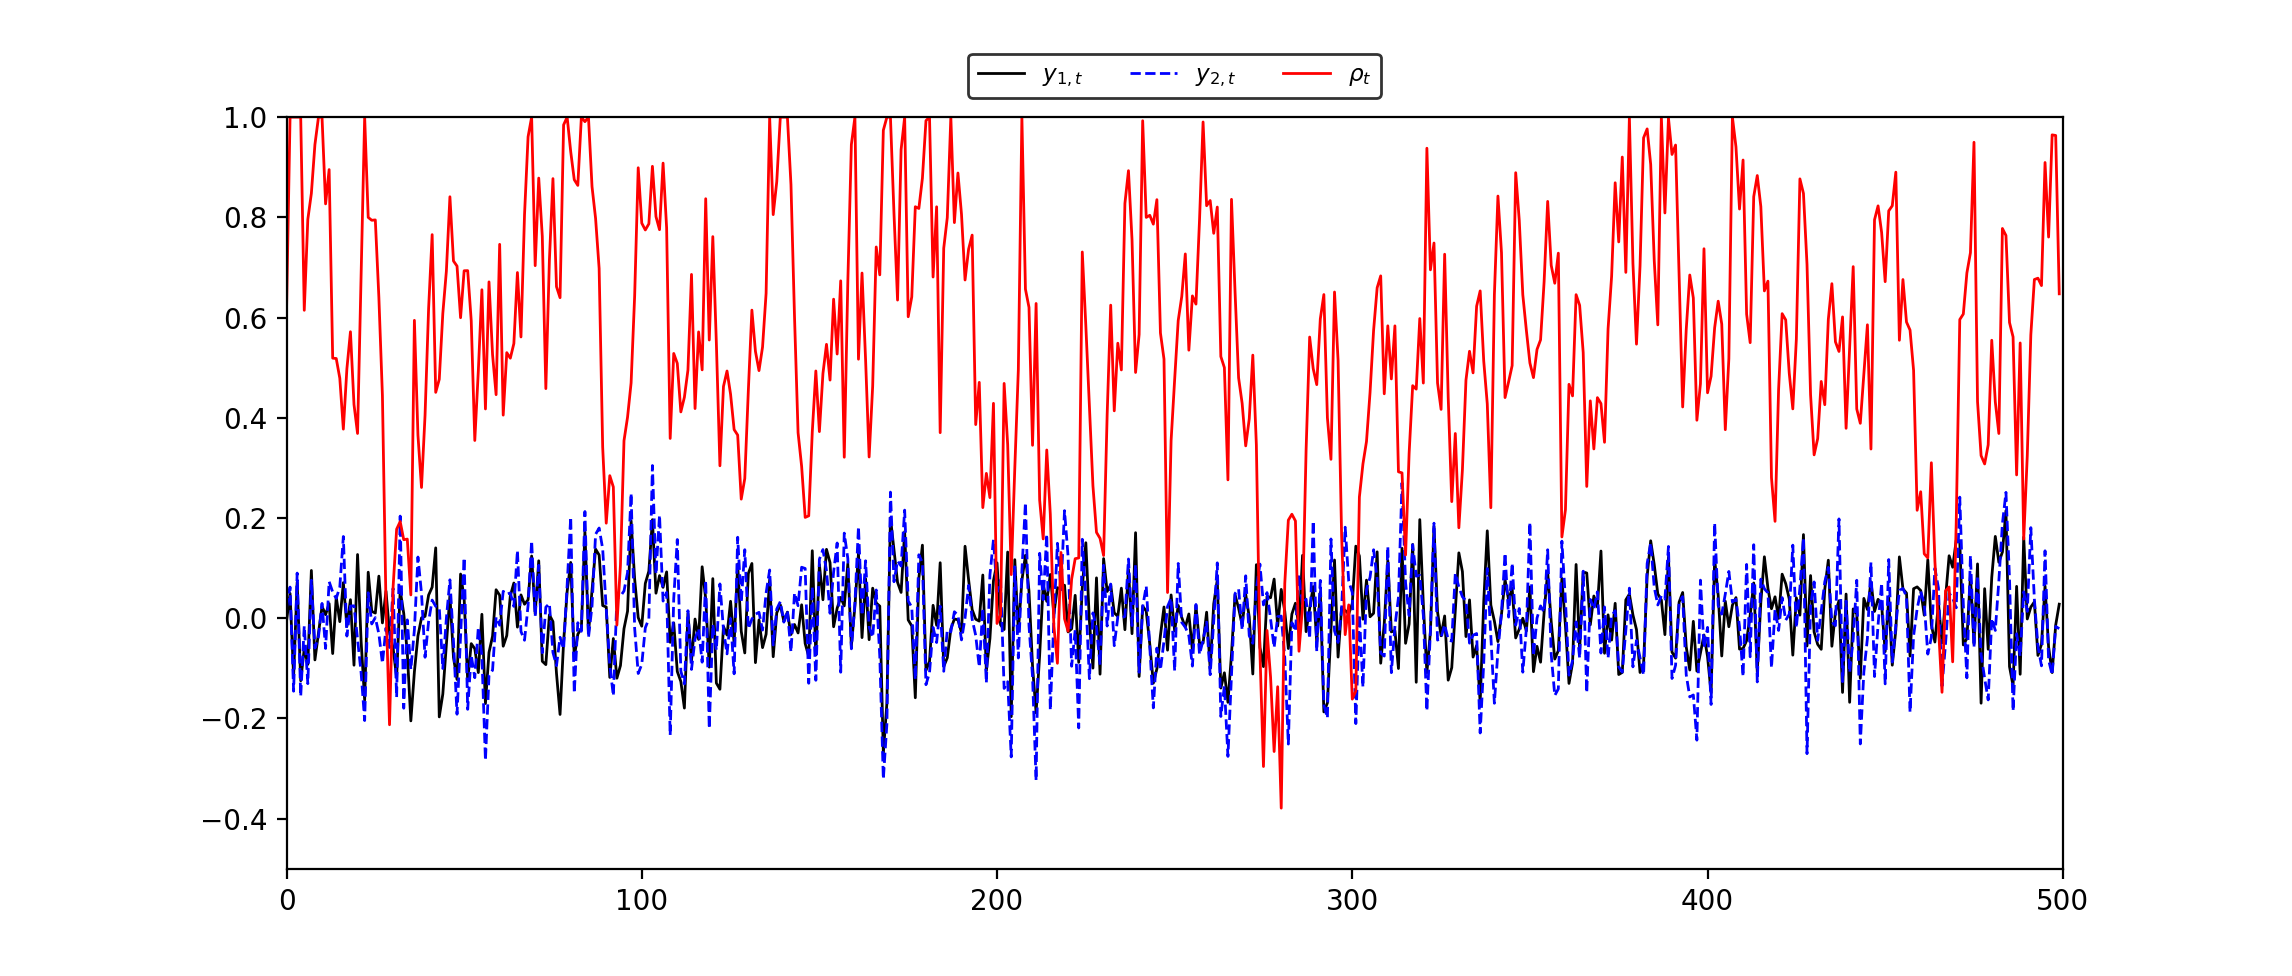
\includegraphics[scale=0.6]{simulation_assetpaths_with_stochastic_correlations.png}
	\caption{Simulated data and time-varying correlation from \eqref{eq:correlation_simulation}.}
	\label{fig:cholesky_simulation}
\end{figure}

\noindent
To assess some of the statistical properties when sample correlation coefficients using moving windows are used as a proxy for true correlation in our supervised learning problem, we will denote the estimation uncertainty associated to the estimated correlation coefficients by the width of their $100(1-\eta)\%$ confidence intervals. These confidence intervals are estimated by application of a bootstrap resampling procedure with replacement: For all time units $t = \{\Delta t, \Delta t +1, \dots, T\}$, for $\Delta t = \{3, 4, \dots, 100\}$, a $1000$ samples of size $\Delta t$ have been randomly selected. For each subsample the correlation coefficient is estimated and, subsequently, the width of the $100(1-\eta)\%$  confidence interval is measured for each coefficient. The parameter $\eta$ is set to $0.01$ in this part of the analysis.    \\ 




\section{Moving Window Estimates of Correlation} \label{sec:MW}
The accuracy of Pearson and Kendall estimates for conditional correlation is compared by using mean squared error ( MSE) between estimated and actual correlations. The variance of mean squared errors from Pearson estimates in Fig. \ref{fig:mse_pearson_kendall_bootstrap} is approximately 1.78e-3 while that of Kendall is approximately 1.59e-3, i.e. Kendall estimates are slightly less sensitive to the choice of window length compared to Pearson estimates but the difference seems negligible small or might even not be significant. Interestingly, it is observed that Kendall estimates for conditional correlation have slightly higher MSE values for larger window lengths. A possible explanation for this observation is that the simulated asset returns follow a multivariate normal distribution, i.e. an elliptical distribution. Therefore, it makes sense that a linear correlation coefficient such as Pearson results in lower MSE values for most window lengths. Pearson can get unreliable in the presence of fat-tailed distributions, which is generally a property of real asset return data \citep{ref:Pozzi2012}. It will be interesting to verify whether Kendall is a better choice for approximation of true correlation in the case of real asset return data in Chapter \ref{chap:multivariate_analysis}. \\

\noindent
Pearson and Kendall moving window estimates of conditional correlation satisfy the positive definiteness condition in the conditional correlation matrix $R_t$ for all time $t$ under all choices of window length. Fig. \ref{fig:det_pearson_kendall} presents the obtained minimum determinants of $R_t$ for all choices of window length. In fact, \cite{ref:Pozzi2012} give proves that Pearson and Kendall sample correlation using moving windows generally results positive definite correlation matrices.     


\begin{figure}[H]
	\centering
	\begin{subfigure}[b]{0.49 \textwidth}
		\centering 
		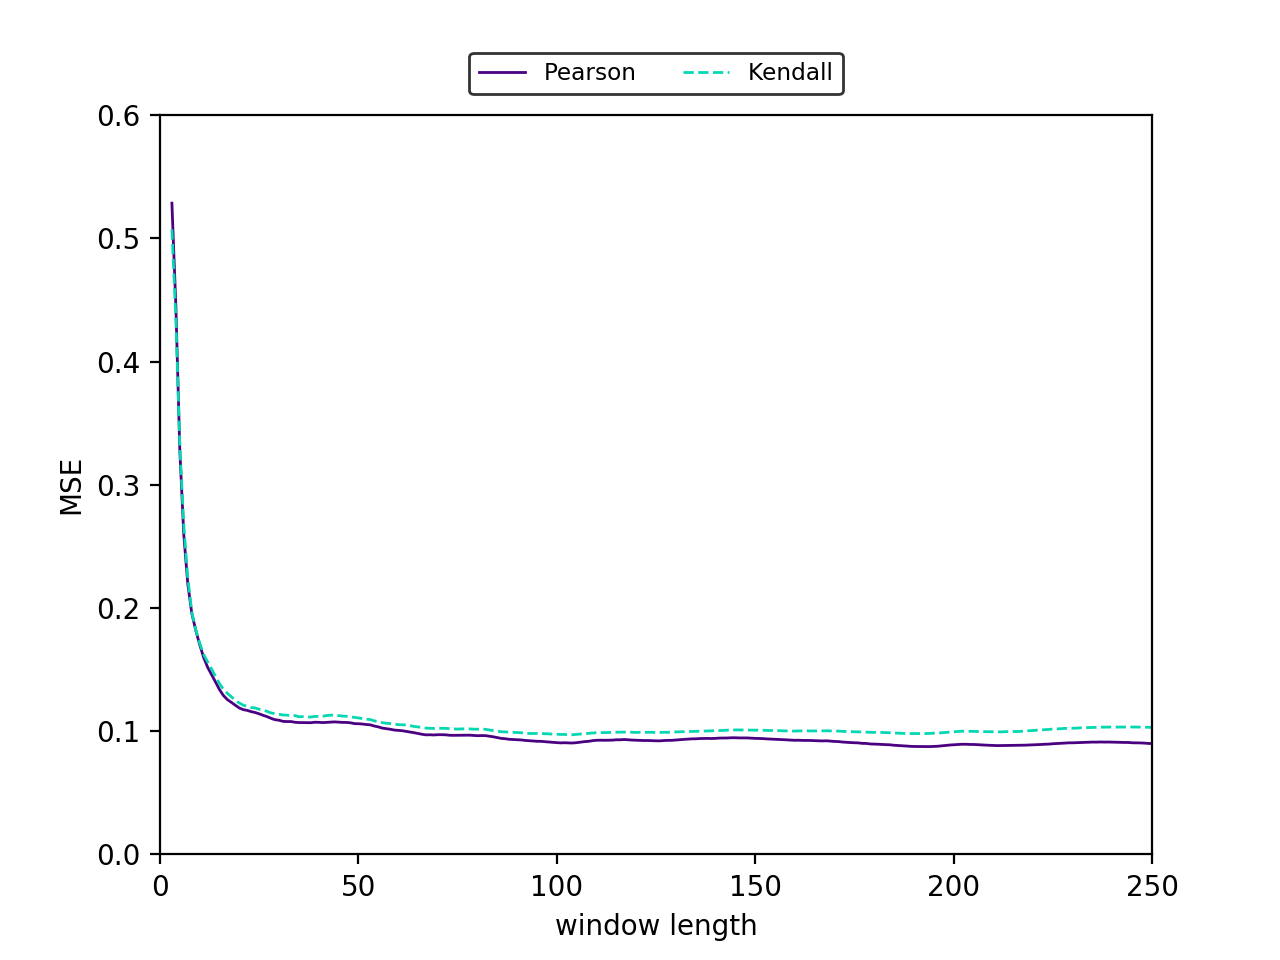
\includegraphics[width=\textwidth]{mse_pearson_kendall.png} 
		\caption{MSE for Pearson and Kendall Moving Window bootstrap estimates.}
		\label{fig:mse_pearson_kendall_bootstrap}
	\end{subfigure}
	\begin{subfigure}[b]{0.49 \textwidth}
		\centering 
		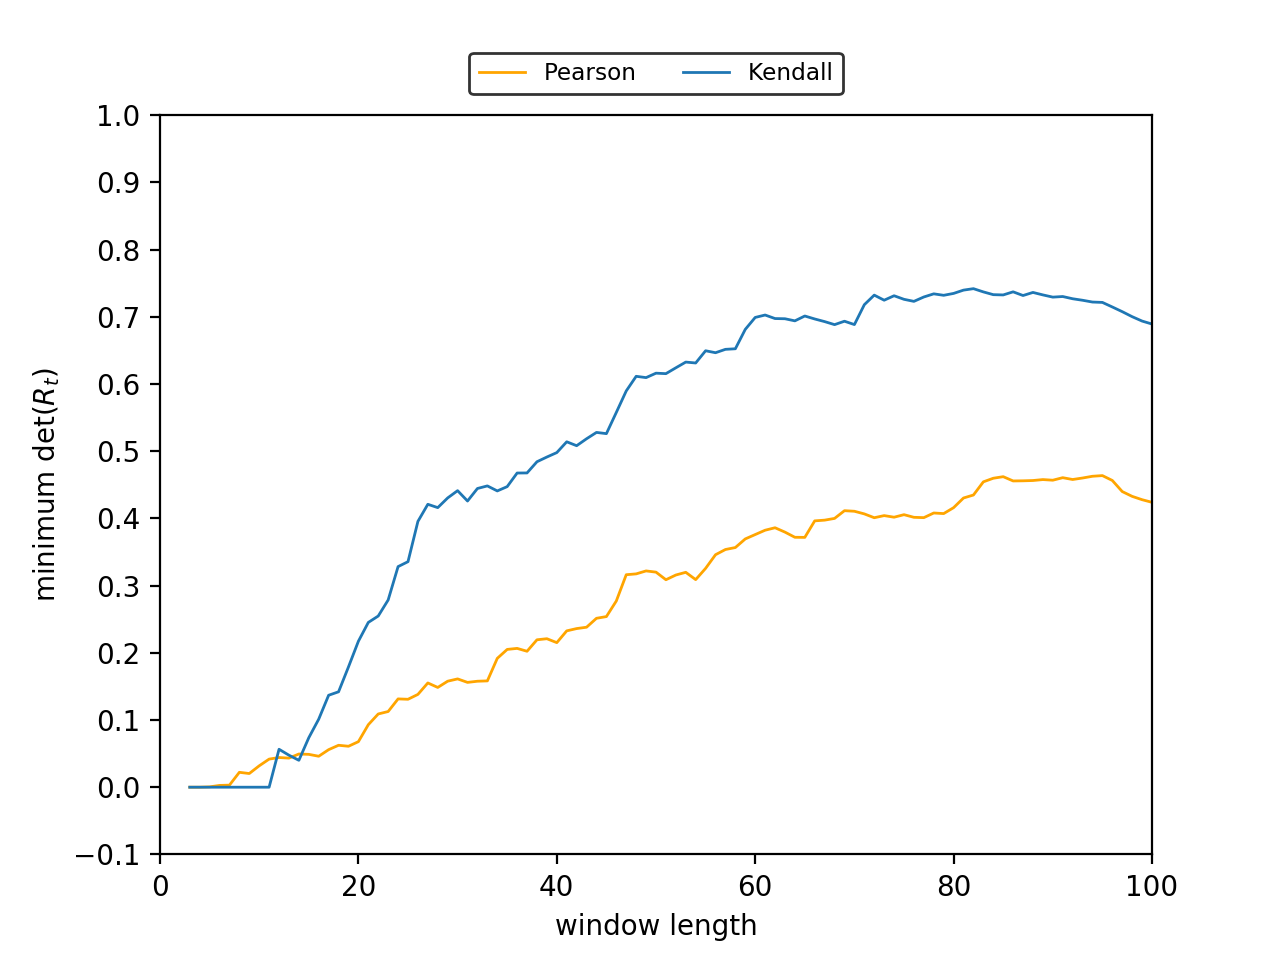
\includegraphics[width=\textwidth]{det_pearson_kendall} 
		\caption{Minimum det($R_t$) from Pearson and Kendall Moving Window bootstrap estimates.}
		\label{fig:det_pearson_kendall}
	\end{subfigure}
	\caption{Comparison MSE and minimum determinants for Pearson and Kendall Moving Window bootstrap estimates\protect\footnotemark.}
	\label{fig:mse_det_pearson_kendall_bootstrap}
\end{figure}


\footnotetext{For Pearson and Kendall correlation approximation using moving window estimates with window sizes 3 through 7 several bootstrapped samples return a standard deviation of zero. This results into NaN values for the associated estimated correlation coefficient as the covariance is divided by zero. These NaN values are excluded for calculation of the mean estimate of Pearson and Kendall correlation coefficient over the test set.} 


\noindent
Fig. \ref{fig:pearson21_bootstrap} and Fig. \ref{fig:kendall21_bootstrap} show that both Pearson and Kendall moving window estimates of correlation change substantially over time indicating the capture of changing correlation levels. Additionally, it is observed that the obtained 99\% confidence intervals around these estimates are rather wide, covering all values in the range $[-1,1]$, which imply that the uncertainty around the estimated values are high \citep{ref:Basturk2016}. Pearson estimates appears to be more volatile than Kendall estimates of correlation, which may be attributed to Kendall's $\tau$ rank correlation's desirable property of being robust to outliers. 

\begin{figure}[H]  % [h] parameter makes sure figures are located at 'this' location.
	\centering
	\begin{subfigure}[b]{0.49 \textwidth} % sum of widths should be less than text width if all one the same line
		\centering 
		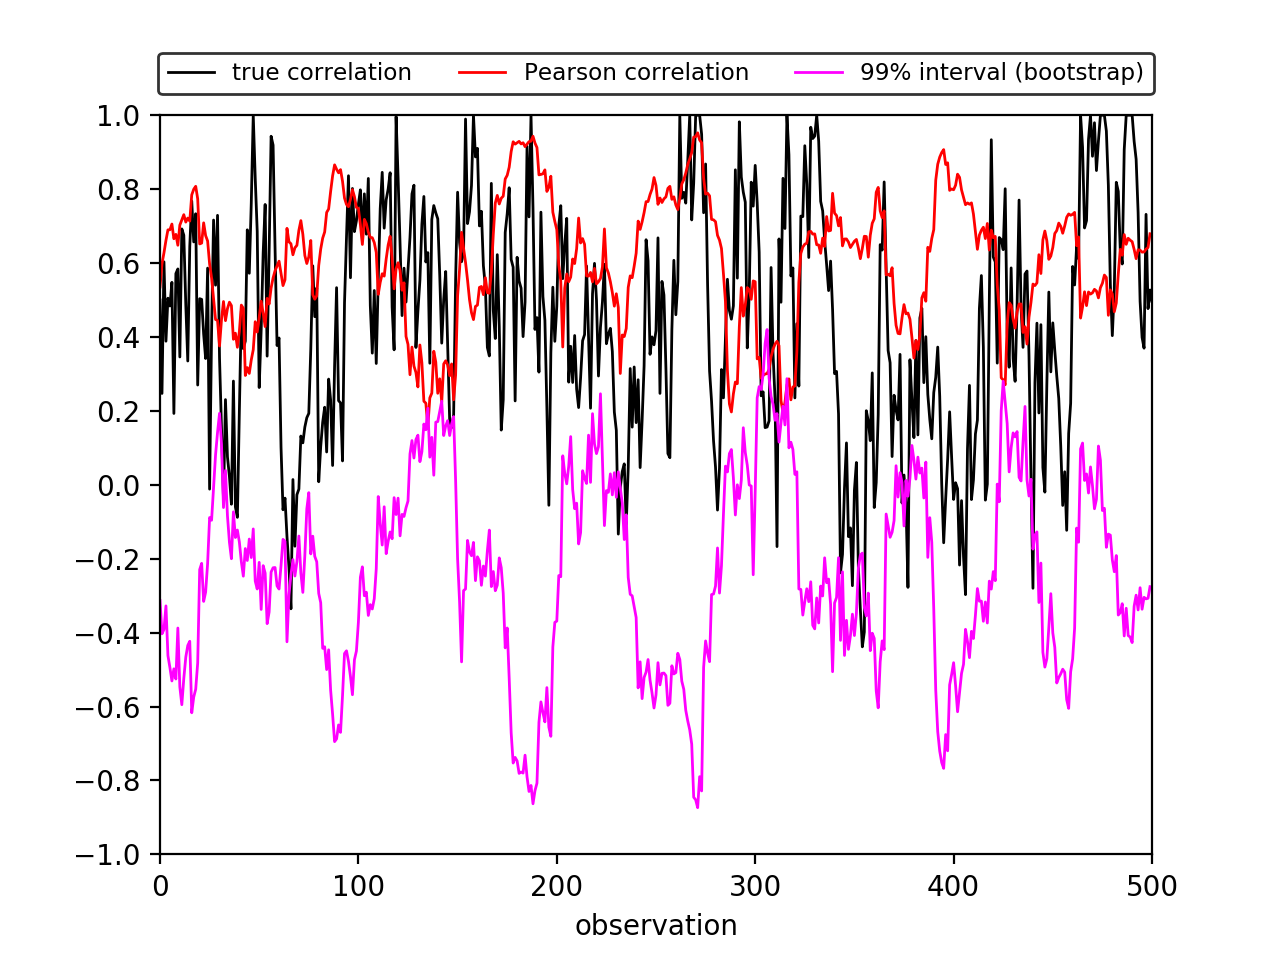
\includegraphics[width=\textwidth]{pearson_21_estimates_bootstrap.png} 
		\caption{Pearson estimates with window size 21.} 		
		\label{fig:pearson21_bootstrap}
	\end{subfigure} 
	\hfill
	\begin{subfigure}[b]{0.49 \textwidth}
		\centering 
		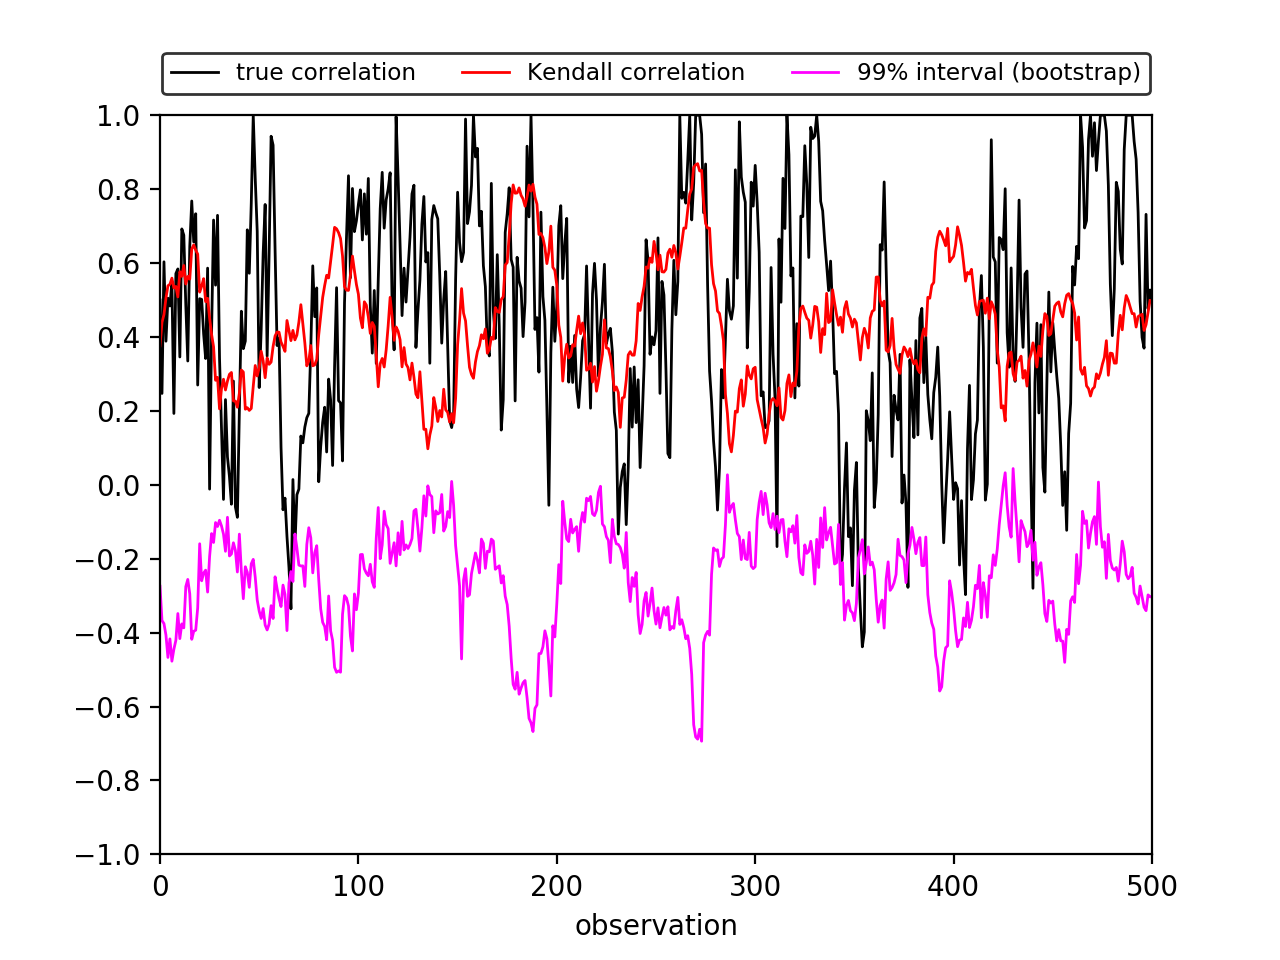
\includegraphics[width=\textwidth]{kendall_21_estimates_bootstrap.png} 
		\caption{Kendall estimates with window size 21.} 		
		\label{fig:kendall21_bootstrap}
	\end{subfigure}
	\hfill
	\begin{subfigure}[b]{0.49 \textwidth} 
		\centering
		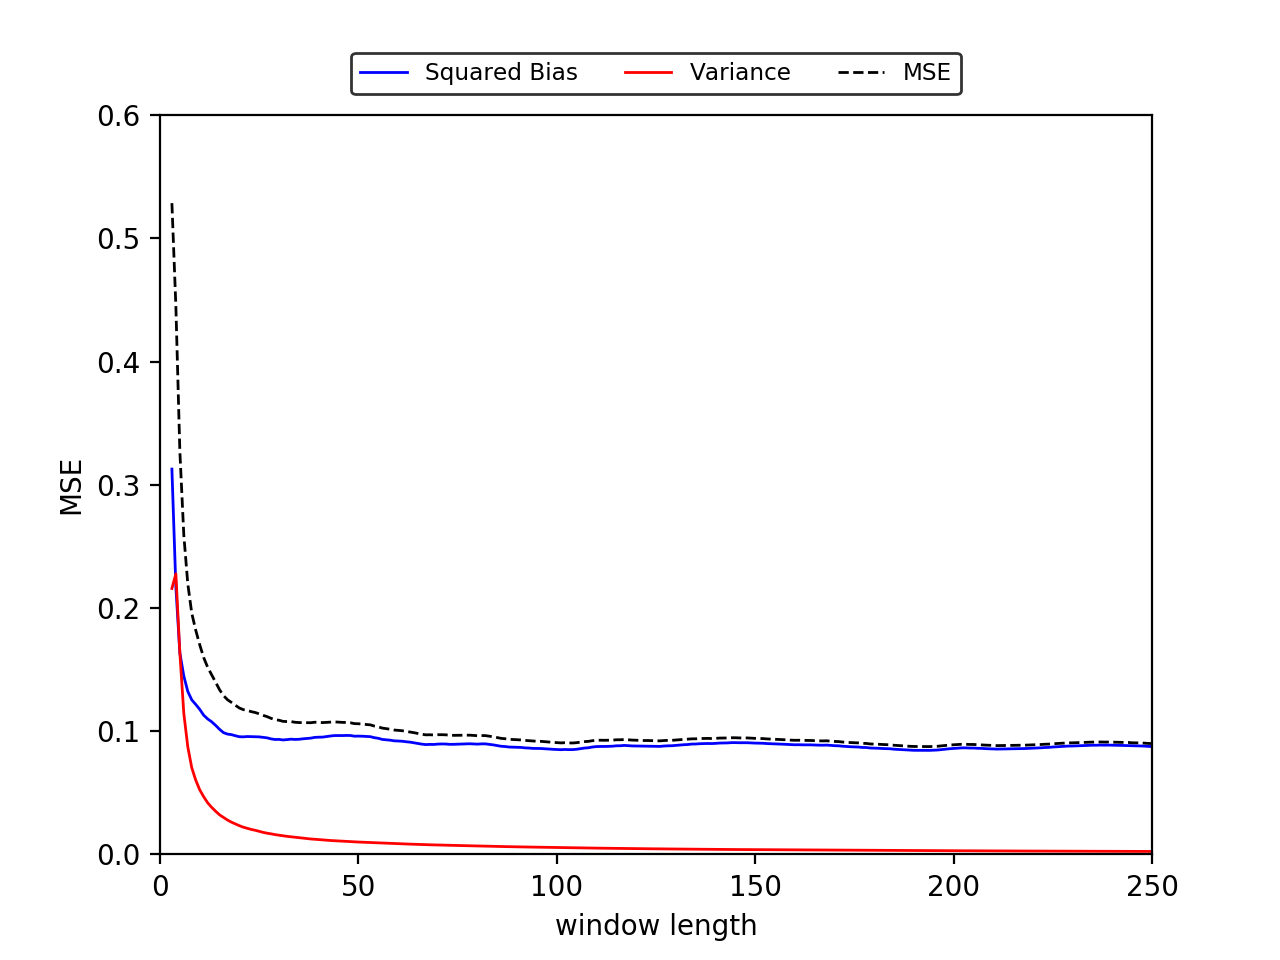
\includegraphics[width=\textwidth]{decom_mse_pearson.png}
		\caption{Bias-variance decomposition for Pearson estimates.}
		\label{fig:decom_mse_pearson}
	\end{subfigure}
	\hfill
	\begin{subfigure}[b]{0.49 \textwidth} 
		\centering
		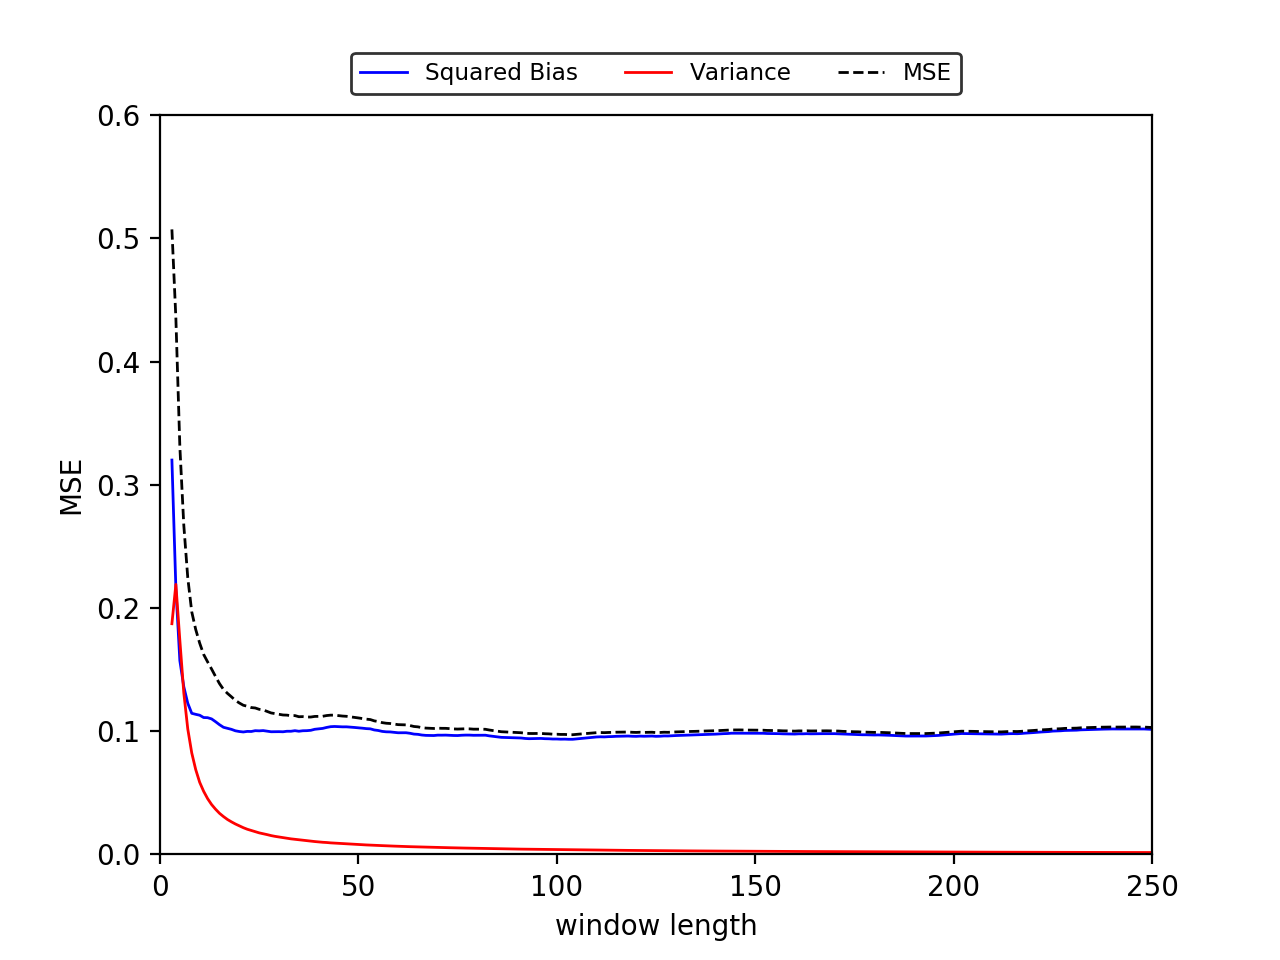
\includegraphics[width=\textwidth]{decom_mse_kendall.png}
		\caption{Bias-variance decomposition for Kendall estimates.}
		\label{fig:decom_mse_kendall}
	\end{subfigure}
	\caption{MSE for Pearson and Kendall Moving Window bootstrap estimates.}
	\label{fig:decom_mse_pearson_kendall_true}
\end{figure}

\noindent
Moreover, Pearson and Kendall estimates using moving windows are very sensitive to the choice of the window length. This is illustrated by the bias-variance decomposition of the MSE between estimated and actual correlations, shown in Fig. \ref{fig:decom_mse_pearson} and Fig. \ref{fig:decom_mse_kendall}. One can observe an inverse relationship between the choice of window length (i.e. the bootstrap sample size) and value of the variance term in the MSE decomposition. This relationship may be explained by the fact that as the bootstrap sample size increases with an increase of the window length, the standard error, or the standard deviation of the sampling distribution, decreases. In other words, as the bootstrap sample size increases, the variability of the sampling distribution decreases which would show through smaller 99\% confidence intervals. Analogously, in these figures this is shown through a decrease in de variance term of the bias-variance decomposition of the MSE between estimated and actual correlations. \\


\section{Learning with True Correlation for Response Variable} \label{sec:true_correlation}
The covariates of proposed nonparametric learning estimators are approximations of true correlation in this section. The response variable is specified as the true correlation as defined by the simulation parameters. Using simulation it is possible to study the effect of using approximations of correlations as covariates on the loss function. \\


%%%%%% NEAREST neighbor TRUE COR %%%%%%%%
\subsection{Generalization Error of Nearest Neighbor under True Correlation} \label{sec:MSE_knn_true}
The accuracy of KNN estimates with Pearson and Kendall covariates for conditional correlation is compared by using the MSE between estimated and actual correlations. MSE from KNN with Pearson and Kendall moving window estimates of correlation for covariates are shown in Fig. \ref{fig:mse_knn5_pearson_kendall_true}. Regardless of the choice of window length, MSE from KNN with Pearson and Kendall covariates are between 0.0939 and 0.1071, and 0.0929 and 0.1071, respectively. The variance of MSE from KNN estimates with Pearson covariates is approximately 6.07e-6 while that of KNN estimates with Kendall covariates is approximately 5.66e-6. KNN thus appears to be insensitive to the choice of window length, regardless whether the set of covariates is constructed from Pearson or Kendall moving window estimates of correlation. KNN's property of insensitivity to the choice of window length is preferred over Pearson and Kendall's property of being highly sensitive to the choice of the window length used for correlation estimates as depicted in Fig. \ref{fig:mse_pearson_kendall_bootstrap}. Moreover, KNN estimates of conditional correlation satisfy the positive definiteness condition in the conditional correlation matrix $R_t$ for all time $t$ under all choices of window length. Fig. \ref{fig:det_knn5_pearson_kendall_true} presents the obtained minimum determinants of $R_t$ for all choices of window length.  
     
\begin{figure}[H]
	\centering
	\begin{subfigure}[b]{0.49 \textwidth} 
		\centering
		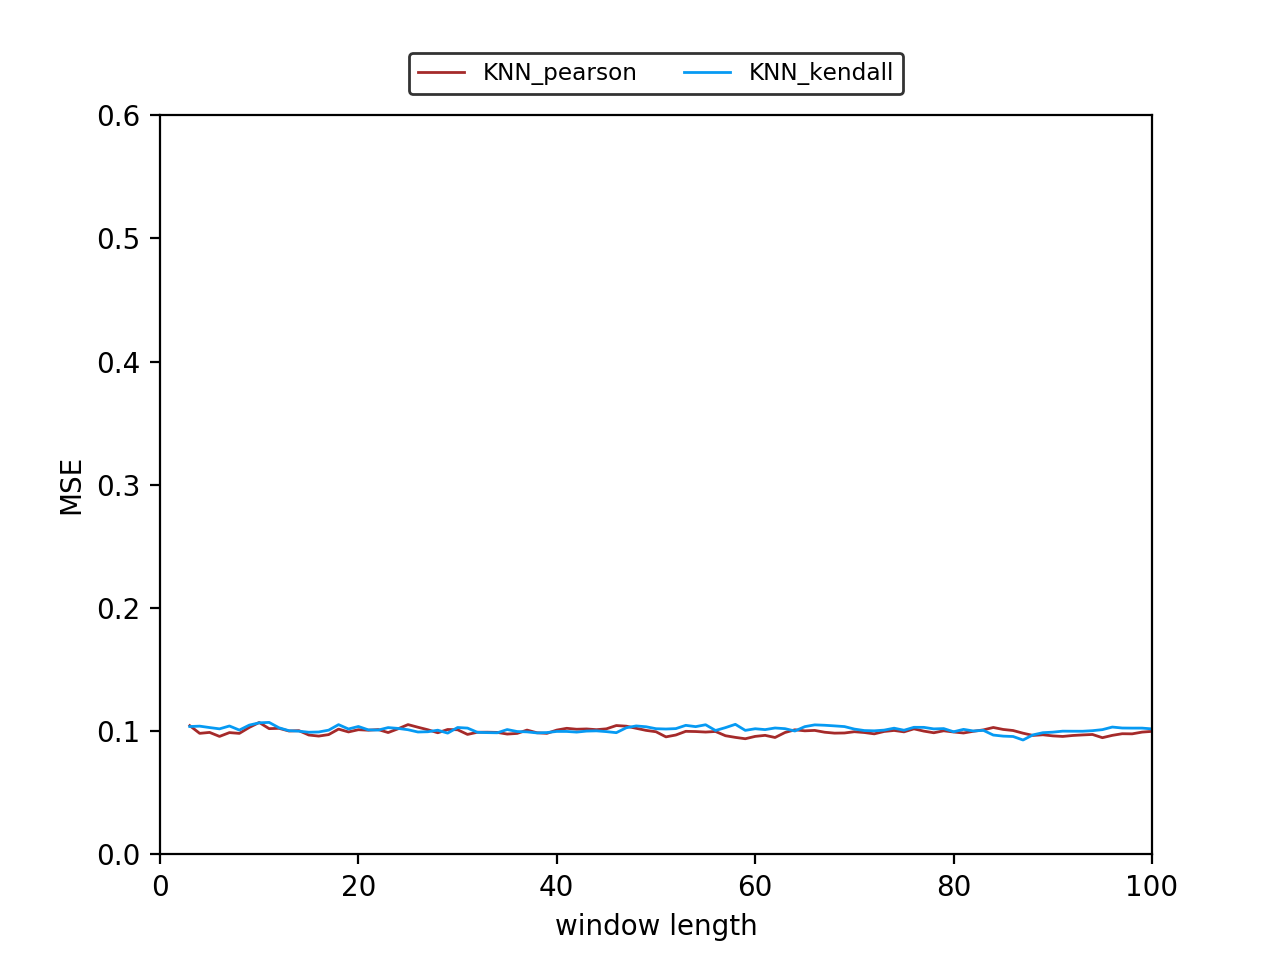
\includegraphics[width=\textwidth]{mse_knn5_pearson_kendall_true.png}
		\caption{MSE for KNN with covariates from Pearson and Kendall and true correlation.}
		\label{fig:mse_knn5_pearson_kendall_true}
	\end{subfigure}
	\hfill
	\begin{subfigure}[b]{0.49 \textwidth} 
		\centering
		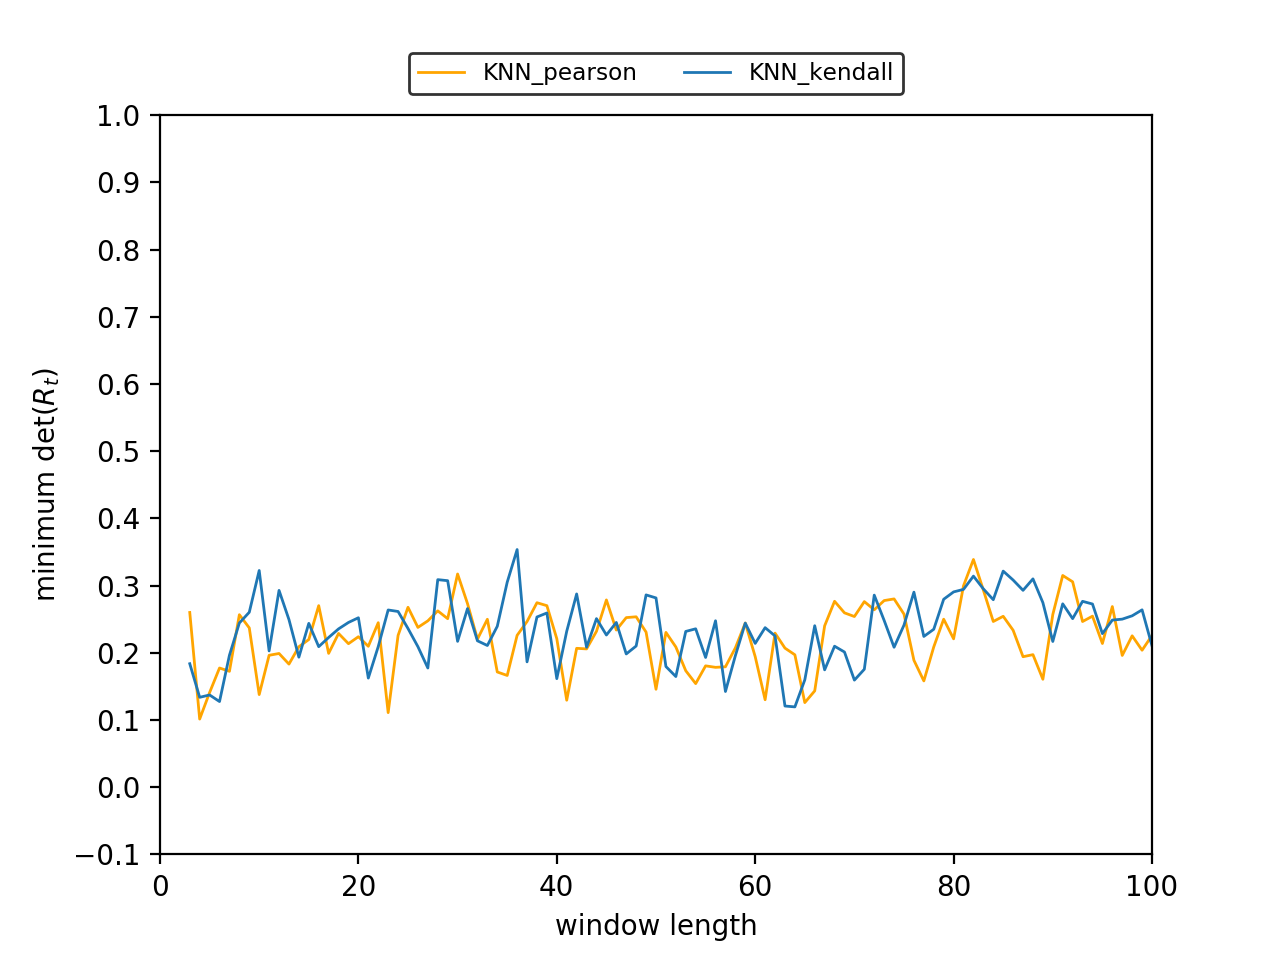
\includegraphics[width=\textwidth]{det_knn5_pearson_kendall_true}
		\caption{Minimum determinants for KNN with covariates from Pearson and Kendall and true correlation.}
		\label{fig:det_knn5_pearson_kendall_true}
	\end{subfigure}
	\caption{Comparison MSE and minimum determinants for KNN(n\_neighbors=5) with covariates from Pearson and Kendall and true correlation.}
	\label{fig:mse_det_knn5_pearson_kendall_true}
\end{figure}


\noindent
From visual inspection of the plots in Fig. \ref{fig:knn_pearson21_bootstrap_true} and Fig. \ref{fig:knn_kendall21_bootstrap_true} it seems that the uncertainty in the conditional correlation, $\rho_t$, which is illustrated by the $99\%$ confidence interval, is smaller for KNN estimates compared to Pearson and Kendall moving window estimates under the same window length of 21. KNN estimates of correlation with number of neighbors equal to 5 are, however, much more volatile. This may be a less desirable result as it is not expected that correlation between assets changes that drastically at each time unit. Rather, correlation is expected to vary gradually over time \citep{ref:Basturk2016}. It is observed though that, as with an increase in the choice of window length for Pearson and Kendall moving window estimates of correlation, an increase in the number of neighbors results in smoother KNN estimates of correlation. \\

\begin{figure}[H]  % [h] parameter makes sure figures are located at 'this' location.
	\centering
	\begin{subfigure}[b]{0.49 \textwidth} % sum of widths should be less than text width if all one the same line
		\centering 
		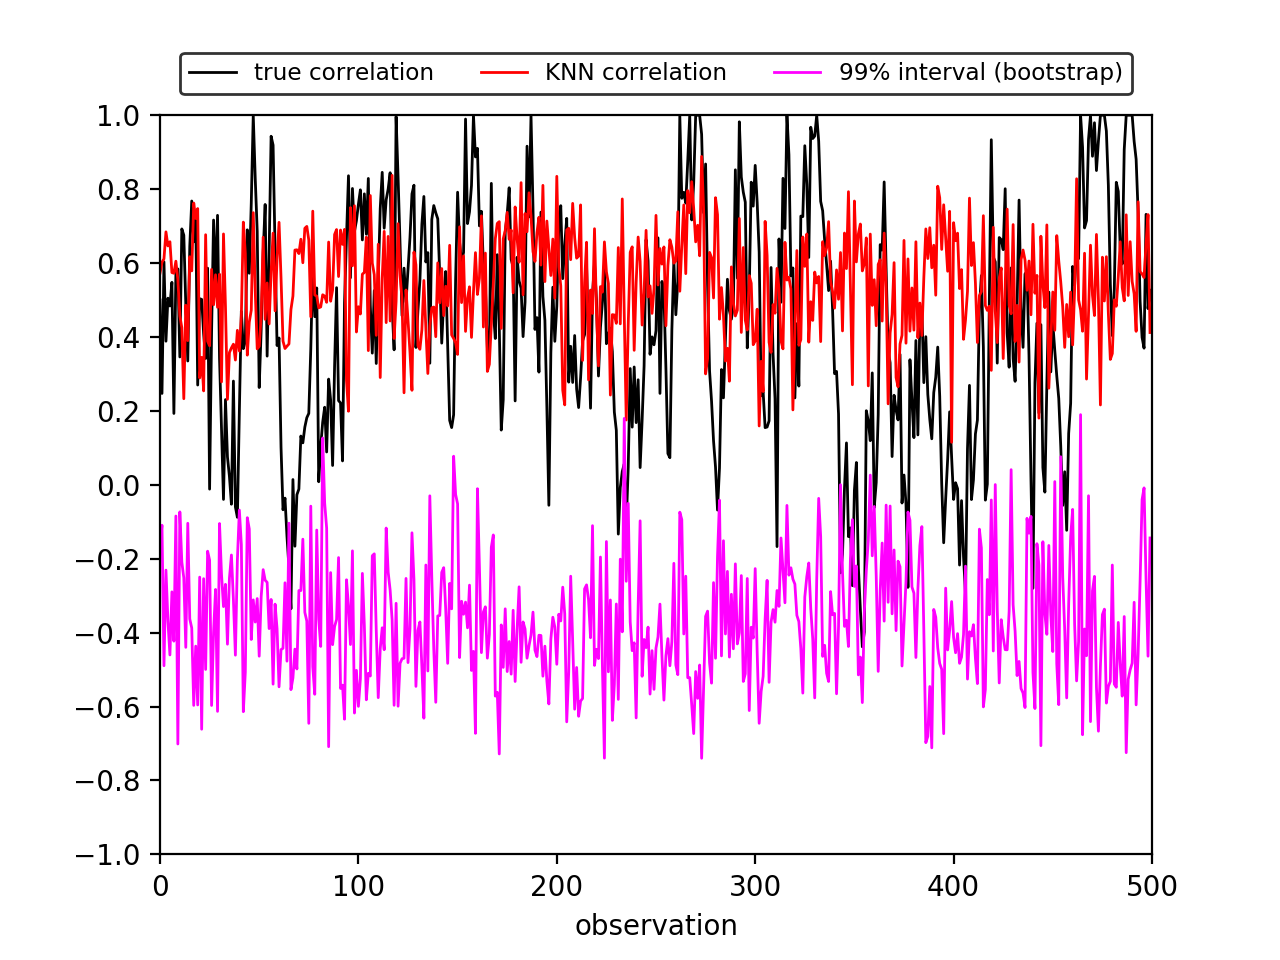
\includegraphics[width=\textwidth]{knn_pearson_21_estimates_bootstrap_true.png} 
		\caption{KNN estimates with window size 21, Pearson as covariate and true correlation.} 	
		\label{fig:knn_pearson21_bootstrap_true}
	\end{subfigure} 
	\hfill	
	\begin{subfigure}[b]{0.49 \textwidth} 
		\centering 
		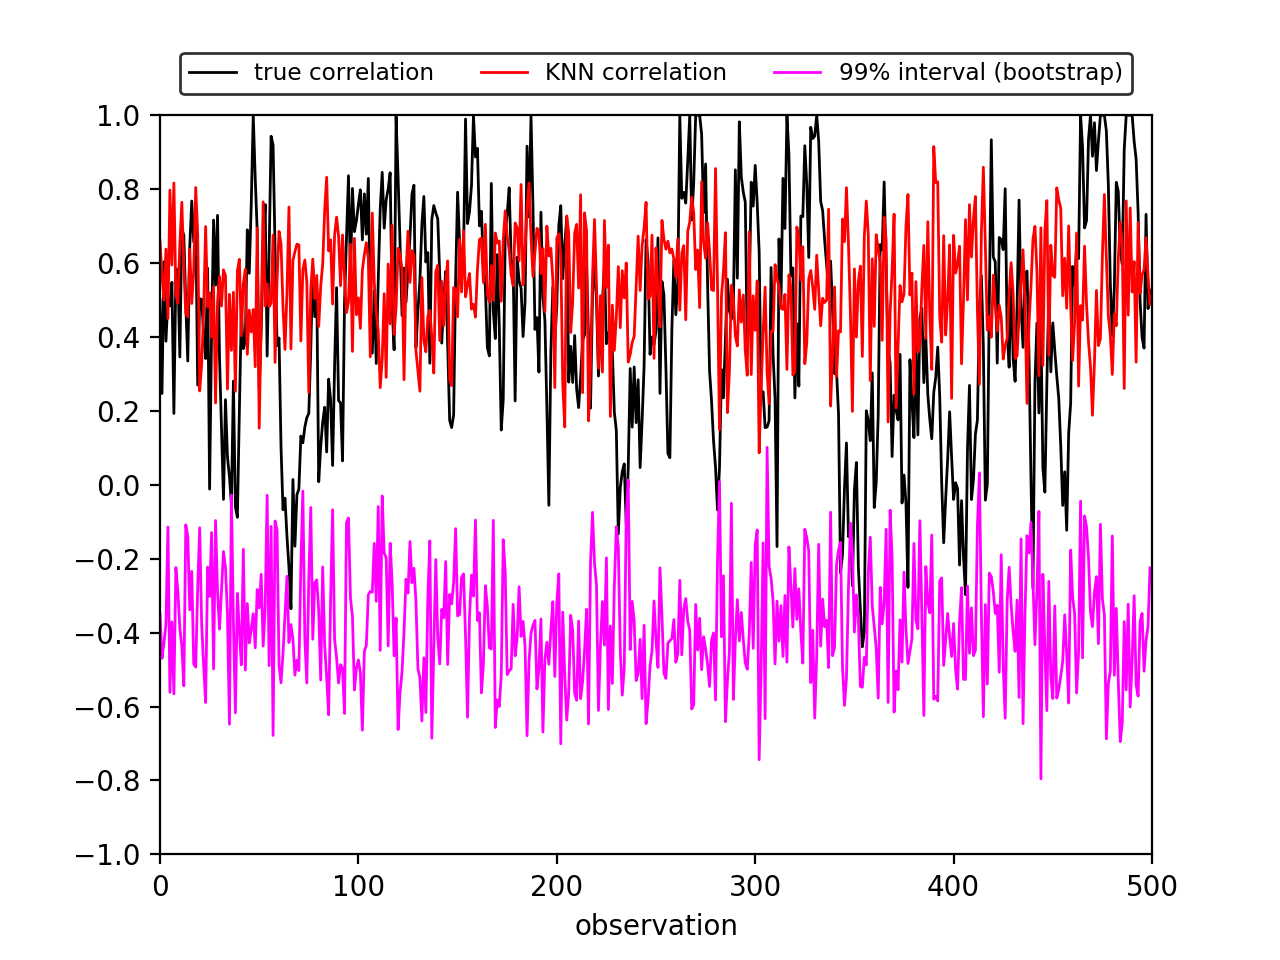
\includegraphics[width=\textwidth]{knn_kendall_21_estimates_bootstrap_true.png} 
		\caption{KNN estimates with window size 21, Kendall as covariate and true correlation.} 
		\label{fig:knn_kendall21_bootstrap_true}
	\end{subfigure} 
	\hfill	
	\begin{subfigure}[b]{0.49 \textwidth}
		\centering 
		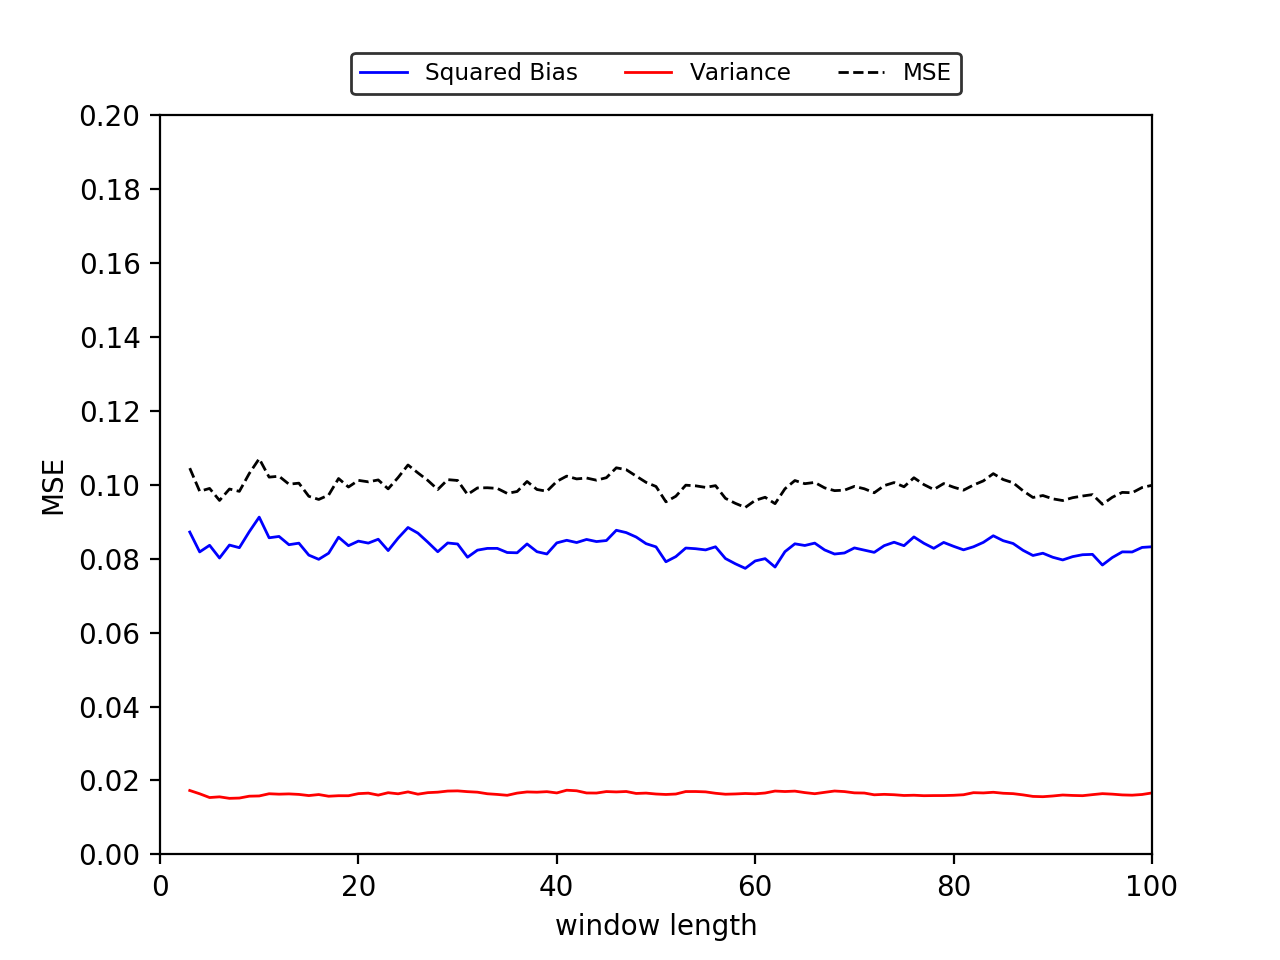
\includegraphics[width=\textwidth]{decom_mse_knn5_pearson_true.png} 
		\caption{Bias-variance decomposition for KNN estimates with Pearson as covariate and true correlation.} 	
		\label{fig:decom_mse_knn5_pearson_true}
	\end{subfigure}
	\hfill  
	\begin{subfigure}[b]{0.49 \textwidth}
		\centering 
		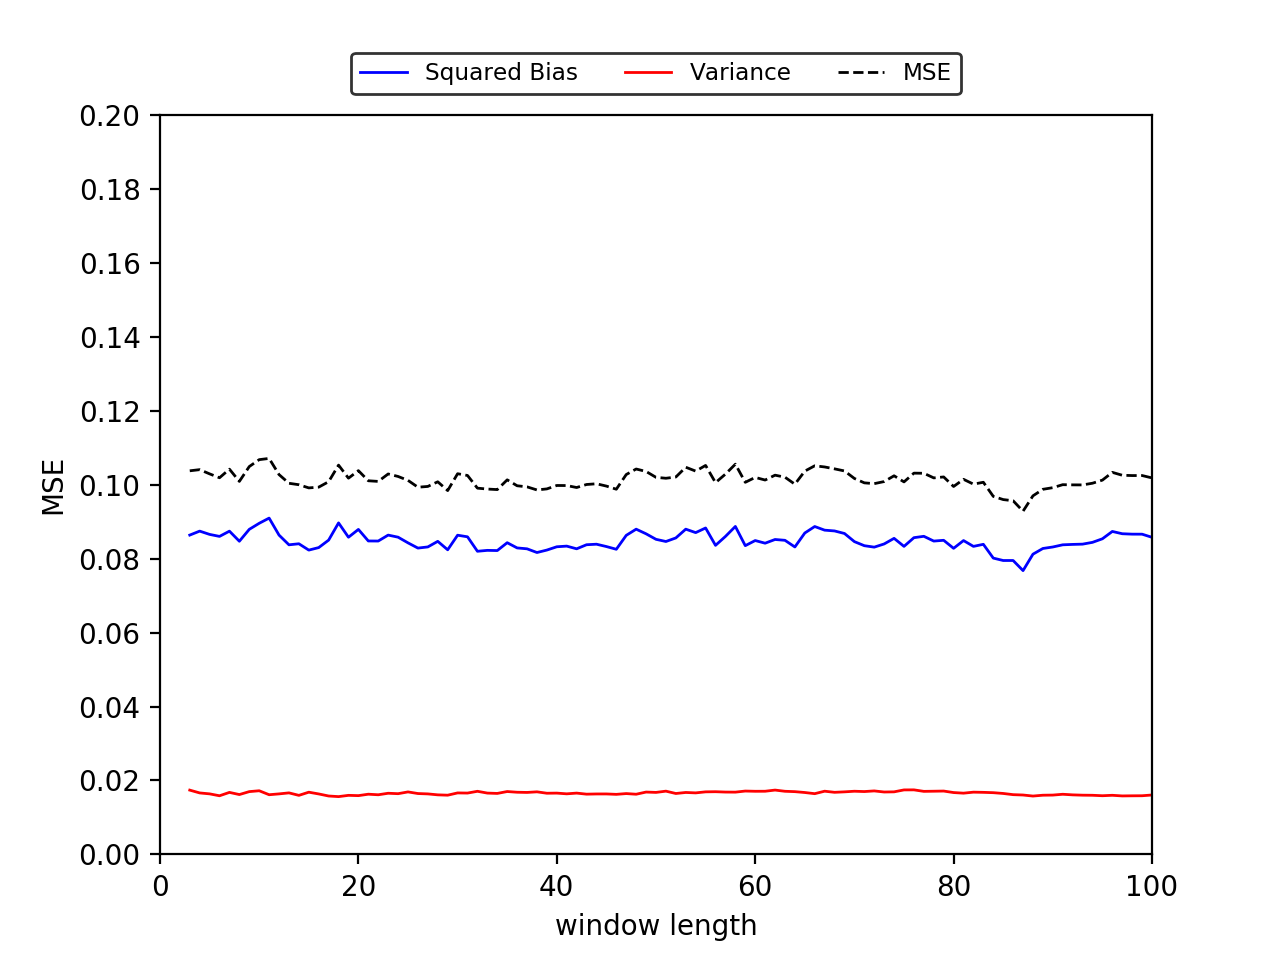
\includegraphics[width=\textwidth]{decom_mse_knn5_kendall_true.png} 
		\caption{Bias-variance decomposition for KNN estimates with Kendall as covariate and true correlation.} 
		\label{fig:decom_mse_knn5_kendall_true}
	\end{subfigure}
	\caption{MSE for KNN estimates with Pearson and Kendall Moving Window bootstrap estimates as covariates and true correlation.}
	\label{fig:decom_mse_knn5_pearson_kendall_true}
\end{figure}

\noindent
The MSE decomposition into bias and variance terms from KNN estimates of correlation are shown in Fig. \ref{fig:decom_mse_knn5_pearson_true} and Fig. \ref{fig:decom_mse_knn5_kendall_true}. These figures indicate that the KNN estimator is considerably less sensitive to the choice of the window length for smaller window sizes when compared to Pearson and Kendall sample correlations using moving windows. The uncertainty around the estimated correlations appears to be marginally affected by the choice of the window length for all window sizes. This statement is supported by the fact that the variance as a function of the window length behaves like a (more or less) constant red line in these figures.   

\subsection{Effect of Alternative Nearest Neighbor Parameterizations under True Correlation} \label{sec:MSE_knn_alt_true}
Fig. \ref{fig:decom_mse_pearson_kendall_true} depicted an inverse relationship between the choice of the window length and the uncertainty around Pearson and Kendall sample correlation estimates using moving windows. The KNN estimator has a similar property: simulation results in Tabel \ref{tab:mse_decomp_knn_pearson_kendall_true} show an inverse relationship between the choice of the number of nearest neighbors used in the estimation of correlations and the uncertainty around the estimated correlations, regardless whether Pearson or Kendall estimates are used for specification of the set of covariates. It is clearly observed that an increase in the number of neighbors, $k$, results in a decrease of the variance, and conversely. This observation is in line with our discussion on MSE decomposition for the KNN estimator and Eq. \eqref{eq:mse_decomposition_knn} in Section \ref{sec:mse_decompose}. Additionally, we stated that the higher the value of $k$, the lower the model complexity and, as such, the squared bias tends to increase with an increase in $k$. However, simulation results depicted in Tabel \ref{tab:mse_decomp_knn_pearson_kendall_true} indicate no increase in squared bias with an increase in $k$ up to $k=800$. The first increase in squared bias is observed when the number of neighbors is approximately 900. For all $k$ smaller than 900 a decrease in squared bias is observed with an increase in $k$. This statement is more clearly shown through a geometrical representation of the MSE decomposition as a function of the number of neighbors for $k \in \{5, 10, 25, 50, 100\}$ in Fig. \ref{fig:knn5_pearson_kendall_sens_analysis_true}. \\  




%% TABLE
\begin{table}[H]
\centering
\captionsetup[subtable]{position=below}
%\captionsetup[table]{position=below}
\begin{subtable}{0.49\linewidth}
\centering
\begin{tabular}{r  c  c  c} 
\toprule
\multicolumn{1}{ r }{\textbf{k}} &
\multicolumn{1}{ c }{\textbf{Squared Bias}} &
\multicolumn{1}{ c }{\textbf{Variance}} &
\multicolumn{1}{ c }{\textbf{MSE}} \\
\midrule 

5                                     & 0.0913                         & 0.0158                & 0.1071     \\
10                                   & 0.0831                         & 0.0087                & 0.0917     \\
25                                   & 0.0785 	                    & 0.0037                & 0.0821     \\
50                                   & 0.0781                         & 0.0018                & 0.0799     \\
100                                 & 0.0785                         & 9.23e-4               & 0.0794      \\
200                                 & 0.0776                         & 4.62e-4               & 0.0781      \\
400                                 & 0.0768                         & 2.31e-4               & 0.0770      \\
600                                 & 0.0757                         & 1.55e-4               & 0.0759     \\
800                                 & 0.0756                         & 1.18e-4               & 0.0757      \\
900				     & 0.0761			   & 1.06e-4              & 0.0760      \\
1000                               & 0.0767                         &  9.70e-5              & 0.0768     \\ [1ex]
\bottomrule
\end{tabular}
\caption{MSE for KNN estimates with window size 10, Pearson as covariate and true correlation.}
\label{tab:mse_decomp_knn_pearson_true}
\end{subtable}
\hfill
\begin{subtable}{0.49\linewidth}
\centering
\begin{tabular}{r  c  c  c} 
\toprule
\multicolumn{1}{ r }{\textbf{k}} &
\multicolumn{1}{ c }{\textbf{Squared Bias}} &
\multicolumn{1}{ c }{\textbf{Variance}} &
\multicolumn{1}{ c }{\textbf{MSE}} \\
\midrule 

5                                     & 0.0896                         &  0.0172               & 0.1068   \\
10                                   & 0.0828                         & 0.0092                & 0.0920   \\
25                                   & 0.0764	                   & 0.0038                & 0.0802    \\
50                                   &  0.0749                        & 0.0019               & 0.0769    \\
100                                 & 0.0749                         & 9.47e-4               & 0.0759    \\
200                                 &  0.0753                        & 4.69e-4              & 0.0757    \\
400                                 &  0.0750                        & 2.37e-4              & 0.0752    \\
600                                 & 0.0749                         & 1.59e-4             & 0.0750     \\
800                                 &   0.0750                       & 1.21e-4             & 0.0751     \\
900				     &  0.0757			   & 1.08e-4             & 0.0758     \\
1000                               &  0.0763                        & 9.80e-5             & 0.0764     \\  [1ex]
\bottomrule
\end{tabular}
\caption{MSE for KNN estimates with window size 10, Kendall as covariate and true correlation.}
\label{tab:mse_decomp_knn_kendall_true}
\end{subtable}
\caption{Mean Squared Error (MSE) decomposition as a function of the number of neighbors (k) for KNN with proxy for covariates and true correlation.}
\label{tab:mse_decomp_knn_pearson_kendall_true}
\end{table}

\noindent
Fig. \ref{fig:knn5_pearson_sens_analysis_true} and Fig. \ref{fig:knn5_kendall_sens_analysis_true}  depict geometrical representations of the simulation results for KNN estimates with Pearson and Kendall covariates (and true correlation), respectively. The MSE decomposition as a function of the number of neighbors for $k \in \{5, 10, 25, 50, 100\}$ clearly shows a decrease in the squared bias with an increase in $k$. Given
Eq. \eqref{eq:mse_decomposition_knn} and our discussion from Section \ref{sec:mse_decompose} one might have expected an increase in squared bias with an increase in $k$. A possible explanation for the behavior depicted in Fig. \ref{fig:knn5_pearson_kendall_sens_analysis_true} may be that up to some $k$, an increase in $k$ implies additional neighbors containing informational value are used for the estimation of conditional correlation. Logically, the inclusion of additional neighbors containing informational value results into more accurate estimates of correlation, which shows through a decrease in squared bias. As of some $k$, additional neighbors only add noise to the estimation process which results into increased squared bias.    

\begin{figure}[H]  % [h] parameter makes sure figures are located at 'this' location.
	\centering
	\begin{subfigure}[b]{0.49 \textwidth} % sum of widths should be less than text width if all one the same line
		\centering 
		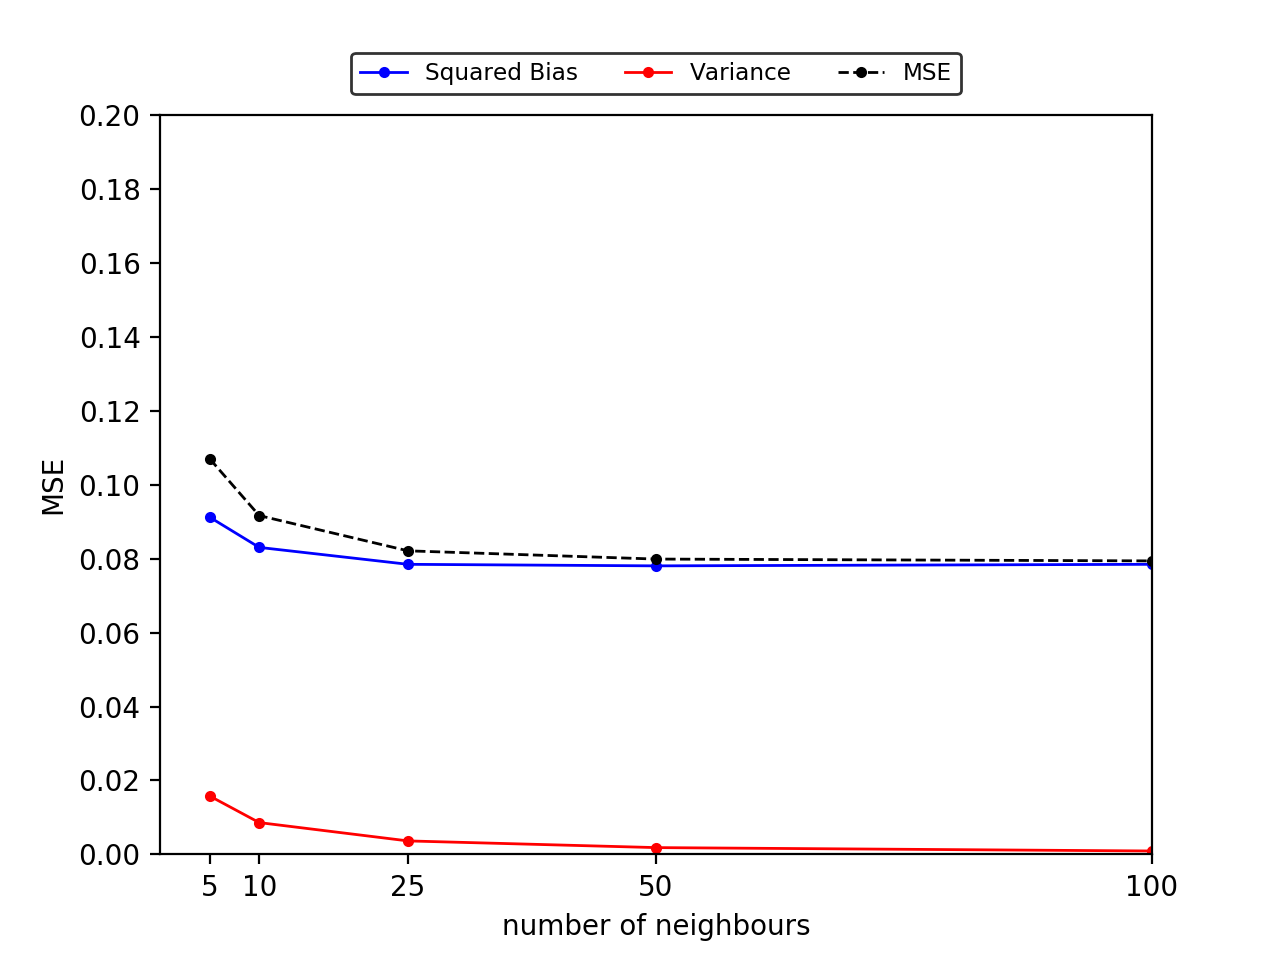
\includegraphics[width=\textwidth]{sens_analysis_mse_knn_pearson_true.png} 
		\caption{KNN estimates with window size 10, Pearson as covariate and true correlation.}
		\label{fig:knn5_pearson_sens_analysis_true}
	\end{subfigure} 
	\hfill	
	\begin{subfigure}[b]{0.49 \textwidth} 
		\centering 
		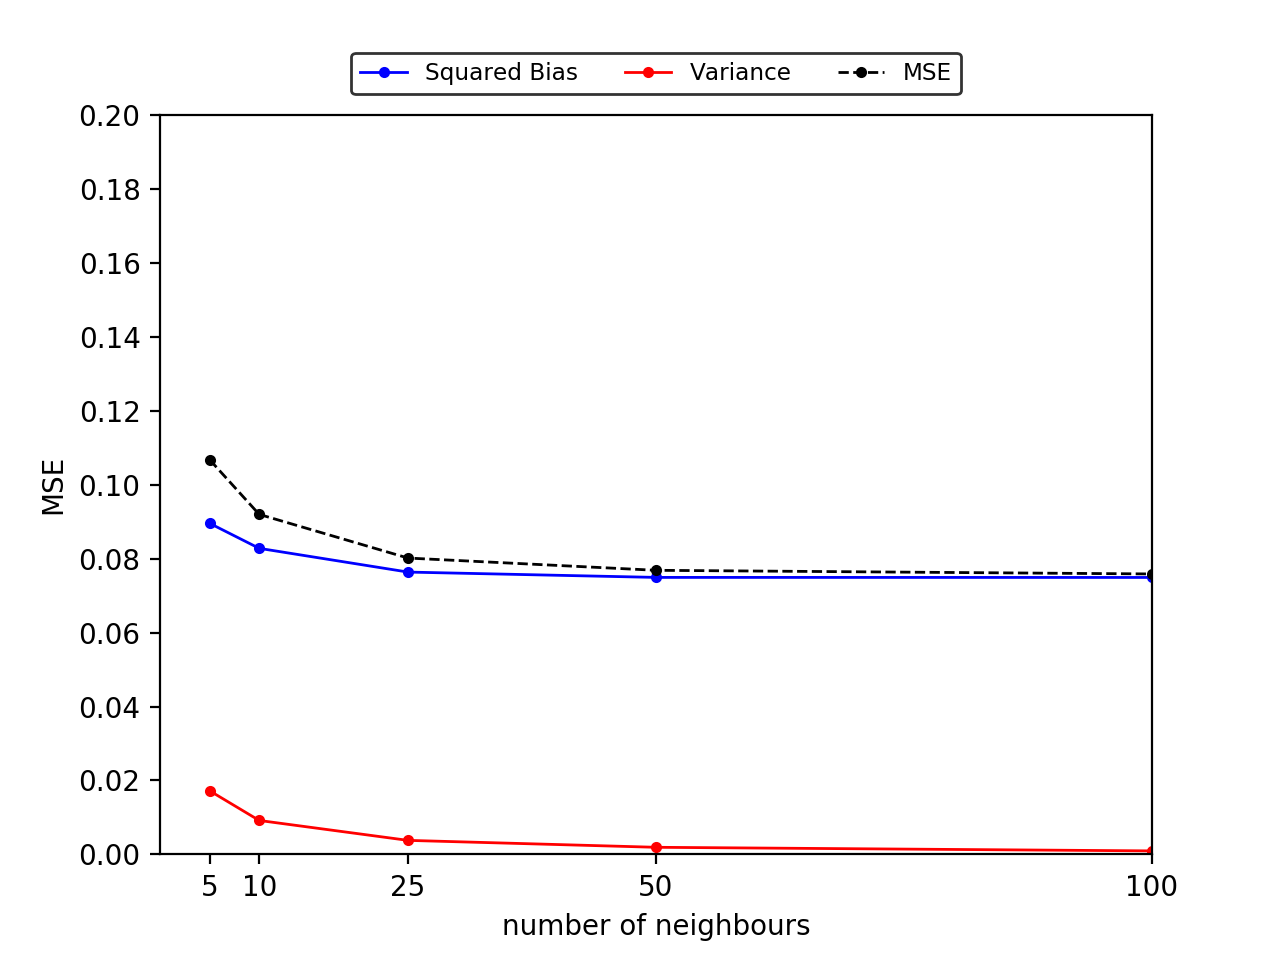
\includegraphics[width=\textwidth]{sens_analysis_mse_knn_kendall_true.png} 
		\caption{KNN estimates window size 10, Kendall as covariate and true correlation.} 
		\label{fig:knn5_kendall_sens_analysis_true}
	\end{subfigure} 
	\caption{MSE as function of number of neighbors for KNN estimates with Pearson and Kendall as covariates and true correlation.}
	\label{fig:knn5_pearson_kendall_sens_analysis_true}
\end{figure}

\noindent
Next, two more parameterizations of the KNN learning algorithm are analyzed. In both parameterizations, the set of neighbors used for point estimation of conditional correlation is defined as the entire training data set. However, in the first parameterization, the KNN estimator uses an uniformly weighted average of correlations where each of the neighbors contributes equally to the point estimate of conditional correlation. In the second parameterization, the KNN estimator uses an inverse distance weighted average of correlations, as defined in \eqref{eq:IDWfunction}. MSE decomposition of both parameterizations with Pearson covariates and true correlation is depicted in Fig. \ref{fig:decom_mse_knn_len_train_IDW_pearson_kendall_true}. Clearly, the variance terms become negligible small in case the set of neighbors used for point estimation of conditional correlation is defined as the entire training data set, regardless of the weighting function. The variance, depicted by the red line, is barely observable in the bottom of Fig. \ref{fig:decom_mse_knn_len_train_pearson_true} and Fig. \ref{fig:decom_mse_knn_IDW_pearson_true}. This observation is in line with results depicted in Tabel \ref{tab:mse_decomp_knn_pearson_kendall_true} where the value of the variance term is negligible small for $k=1000$, regardless whether the set of covariates is constructed from Pearson or Kendall moving window estimates of correlation. \\

\noindent
Although low variance is a desirable property of any estimator, the estimated correlation dynamics depicted in Fig. \ref{fig:decom_mse_knn_len_train_pearson_true} and Fig. \ref{fig:decom_mse_knn_IDW_pearson_true} show very little volatility\footnote{Only behavior of the alternative parameterized KNN estimator with Pearson covariates is shown as behavior of its Kendall counterpart is nearly identical.}. In fact, when the KNN estimator uses an uniformly weighted average of correlations and the entire training data set, the estimated correlation dynamics resemble assuming constant correlation, which is the exact concept we tend to improve on by assuming correlation between financial returns to be conditional. In case of an inverse distance weighting function, the KNN estimator does capture some conditional correlation dynamics resulting in low volatile and smooth correlation dynamics. In reality, the underlying correlation dynamics may potentially be best captured optimizing over the hyperparmeter $k$ until an appropriate level of volatility and smoothness is reached.              \\      

\begin{figure}[H]  % [h] parameter makes sure figures are located at 'this' location.
	\centering
	\begin{subfigure}[b]{0.49 \textwidth}
		\centering 
		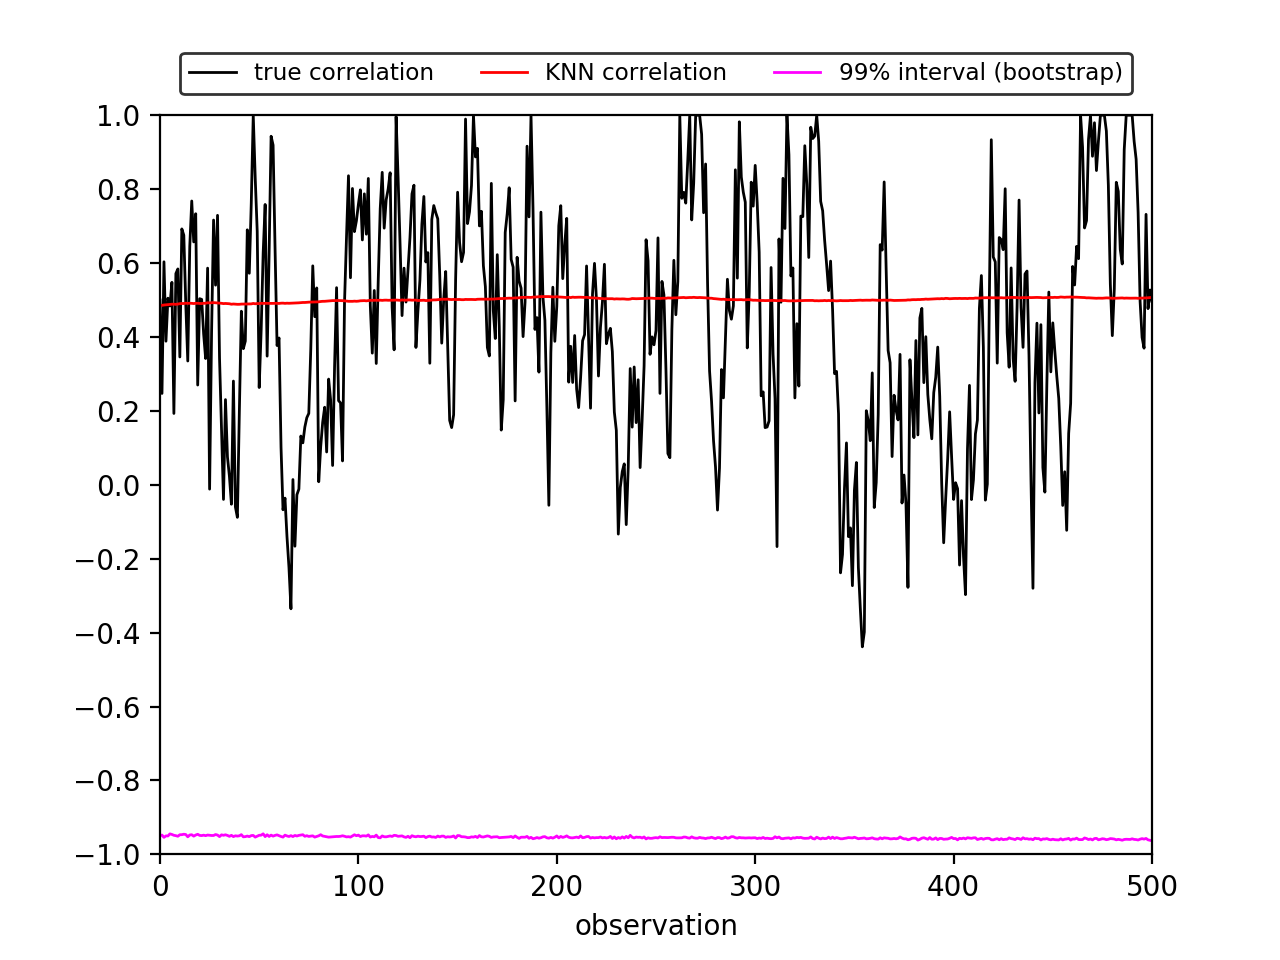
\includegraphics[width=\textwidth]{knn_pearson_21_len_train_estimates_bootstrap_true.png} 
		\caption{KNN estimates as uniformly weighted averages, with window size 21 and Pearson covariates.} 	
		\label{fig:knn_pearson21_len_train_bootstrap_true}
	\end{subfigure}
	\hfill  
	\begin{subfigure}[b]{0.49 \textwidth}
		\centering 
		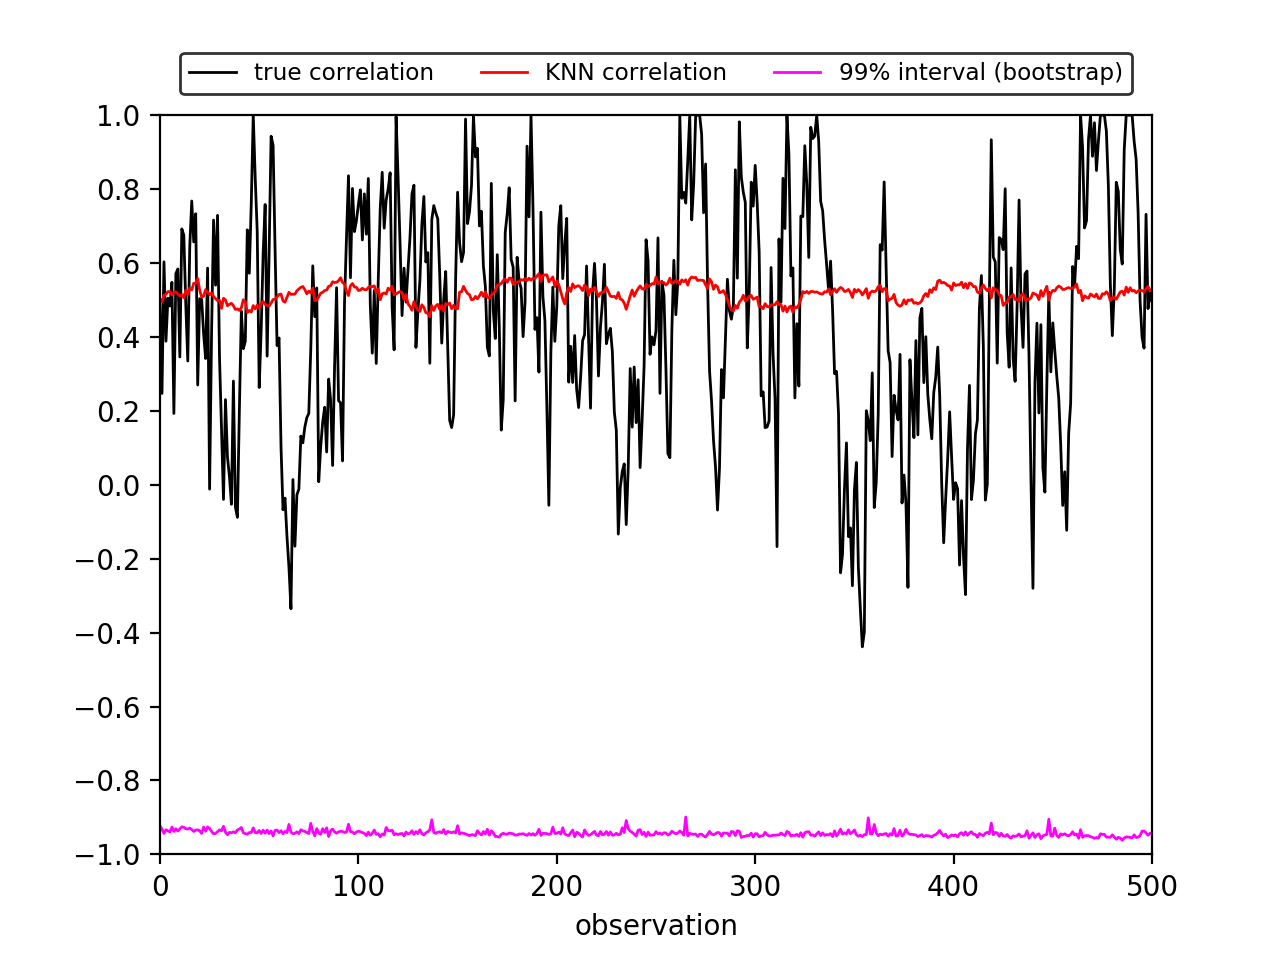
\includegraphics[width=\textwidth]{knn_pearson_21_IDW_estimates_bootstrap_true.png} 
		\caption{KNN estimates as inverse distance weighted averages, with window size 21 and Pearson covariates.} 
		\label{fig:knn_pearson21_IDW_bootstrap_true}
	\end{subfigure}

	\begin{subfigure}[b]{0.49 \textwidth}
		\centering 
		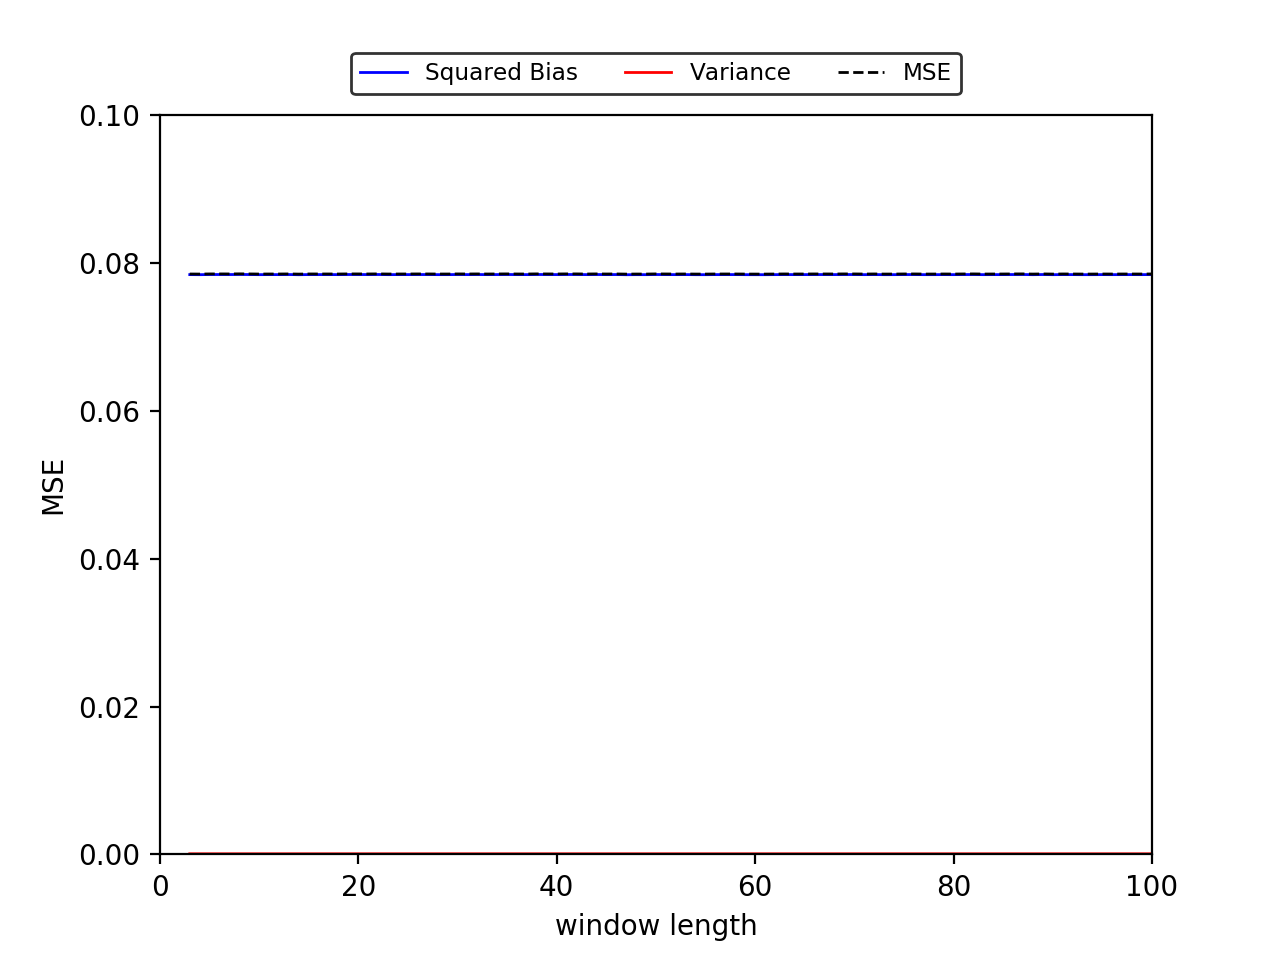
\includegraphics[width=\textwidth]{decom_mse_knn_len_train_pearson_true.png} 
		\caption{Bias-variance decomposition for KNN estimates constructed from uniformly weighted averages.} 	
		\label{fig:decom_mse_knn_len_train_pearson_true}
	\end{subfigure}
	\hfill  
	\begin{subfigure}[b]{0.49 \textwidth}
		\centering 
		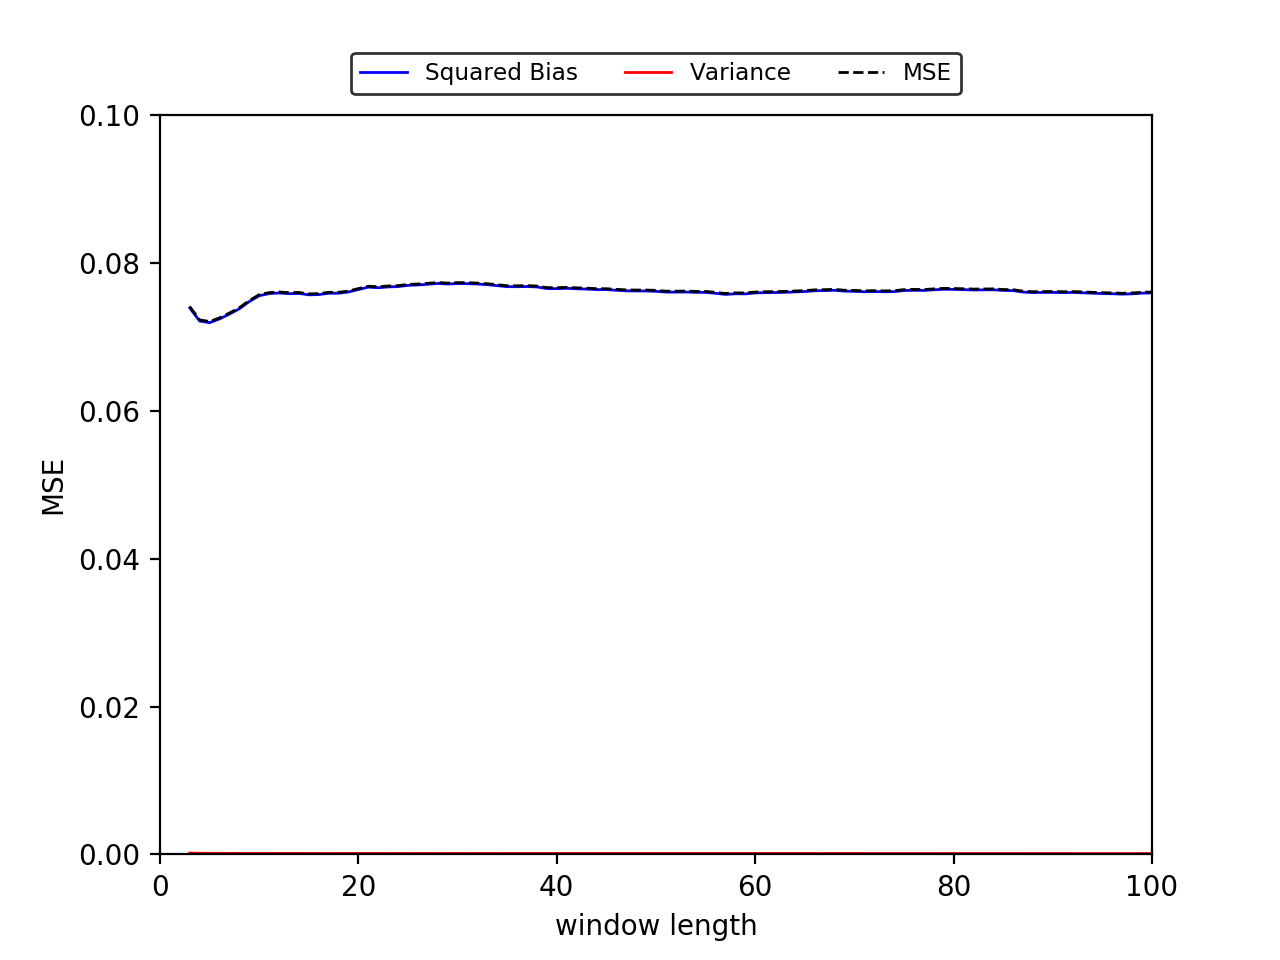
\includegraphics[width=\textwidth]{decom_mse_knn_IDW_pearson_true.png} 
		\caption{Bias-variance decomposition for KNN estimates constructed from inverse distance weighted averages.} 
		\label{fig:decom_mse_knn_IDW_pearson_true}
	\end{subfigure}
	\caption{MSE for KNN estimates with different weighting functions, Pearson Moving Window bootstrap estimates as covariates and true correlation.}
	\label{fig:decom_mse_knn_len_train_IDW_pearson_kendall_true}
\end{figure}

\noindent
The accuracy of the two different parameterizations is compared using MSE between estimated and actual correlations. In Fig. \ref{fig:decom_mse_knn_len_train_pearson_true}, MSE from KNN with an uniform weighting function is approximately 0.0785, regardless of the choice of window length and whether Pearson or Kendall moving window estimates are use for constructing the set of covariates. In Fig. \ref{fig:decom_mse_knn_IDW_pearson_true} MSE from KNN with an inverse distance weighting function is approximately between 0.0721 and 0.0774, and between 0.0727 and 0.0771 when Pearson and Kendall moving window estimates are used as covariates, respectively. This implies that slightly lower MSE values are obtained with an inverse distance weighting function as opposed to an uniform weighting function, which is line with our discussion from Section \ref{sec:knn}. It makes sense to have training data instances with a higher amount of proximity to the query instance contribute more to the value of the response variable than training data instances with a lower amount of proximity to the query instance. Moreover, Fig. \ref{fig:decom_mse_knn_len_train_IDW_pearson_kendall_true} shows that both parameterizations are insensitive to the choice of window length, regardless of the weighting function and covariate choice. In fact, the variance of MSE from KNN with an uniform weighting function and an inverse distance weighting function are 5.00e-11 and 8.55e-7, respectively. In other words, hardly significantly different from one another. \\

\noindent
The alternative parameterizations of the KNN estimator with approximated covariates and response variable also satisfy the positive definiteness condition of the conditional correlation matrix $R_t$ for all time $t$ under all choices of window length in the interval [0, 100]. Fig. \ref{fig:det_knn_IDW_pearson_kendall_true.png} presents the obtained minimum determinants of $R_t$ for all choices of window length under an inverse distance weighting function\footnote{Usage of an uniform distance weighting function yields approximately constant minimum determinant of 0.74, for both Pearson and Kendall approximations.}.  \\ 

\noindent
This section is concluded with a comparison of the function approximation capabilities of the KNN estimator and Pearson and Kendall sample correlation estimates using moving windows. Comparison is based on MSE between estimated and actual correlations. Fig. \ref{fig:mse_knn5_idw_pearson_kendall_true} shows MSE from KNN under a default parameterization where the number of neighbors equals 5, an alternative parameterization with an inverse distance weighting function as well as Pearson and Kendall moving window estimates of conditional correlations. According to MSE, parameterizations of the KNN estimator where the number of neighbors is 5 or 10 perform better than those of Pearson and Kendall moving window estimates for small window sizes. Parameterizations of the KNN estimator with an alternative distance weighting function and where the entire training data set is used for estimating correlation yields significantly smaller MSE compared to Pearson and Kendall sample correlation estimates using moving windows for all window sizes. In fact, the simulation shows that the KNN estimator outperforms Pearson and Kendall sample correlation estimates for all window sizes when the number of neighbors $k \in \{25, 50, 100\}$ in addition to both alternative parameterizations. Finally, the variance of MSE from KNN estimates under default parameterizations and with an inverse distance weighting function in Fig. \ref{fig:mse_knn5_idw_pearson_kendall_true} are 6.07e-6 and 8.55e-7, respectively, while that of Pearson and Kendall sample correlation estimates using moving windows are 0.0040 and 0.0037, respectively. \\


\begin{figure}[H]  % [h] parameter makes sure figures are located at 'this' location.
	\centering
	\begin{subfigure}[b]{0.49 \textwidth}
		\centering 
		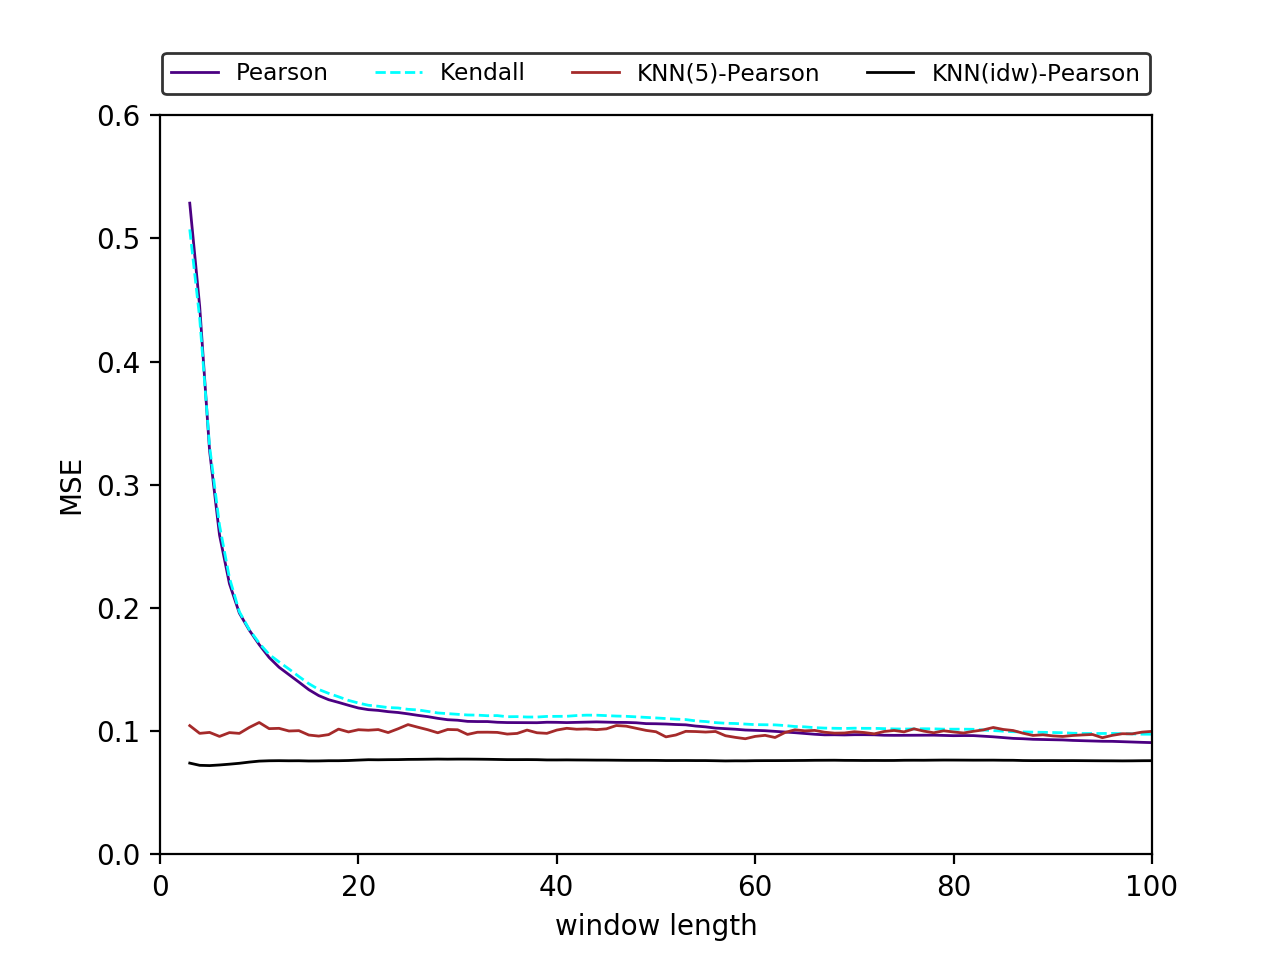
\includegraphics[width=\textwidth]{mse_knn5_idw_pearson_kendall_true} 
		\caption{MSE for KNN with Pearson covariates and true correlation, Pearson and Kendall Moving Window bootstrap estimates.}
		\label{fig:mse_knn5_idw_pearson_kendall_true}
	\end{subfigure}
	\hfill
	\begin{subfigure}[b]{0.49 \textwidth}
		\centering 
		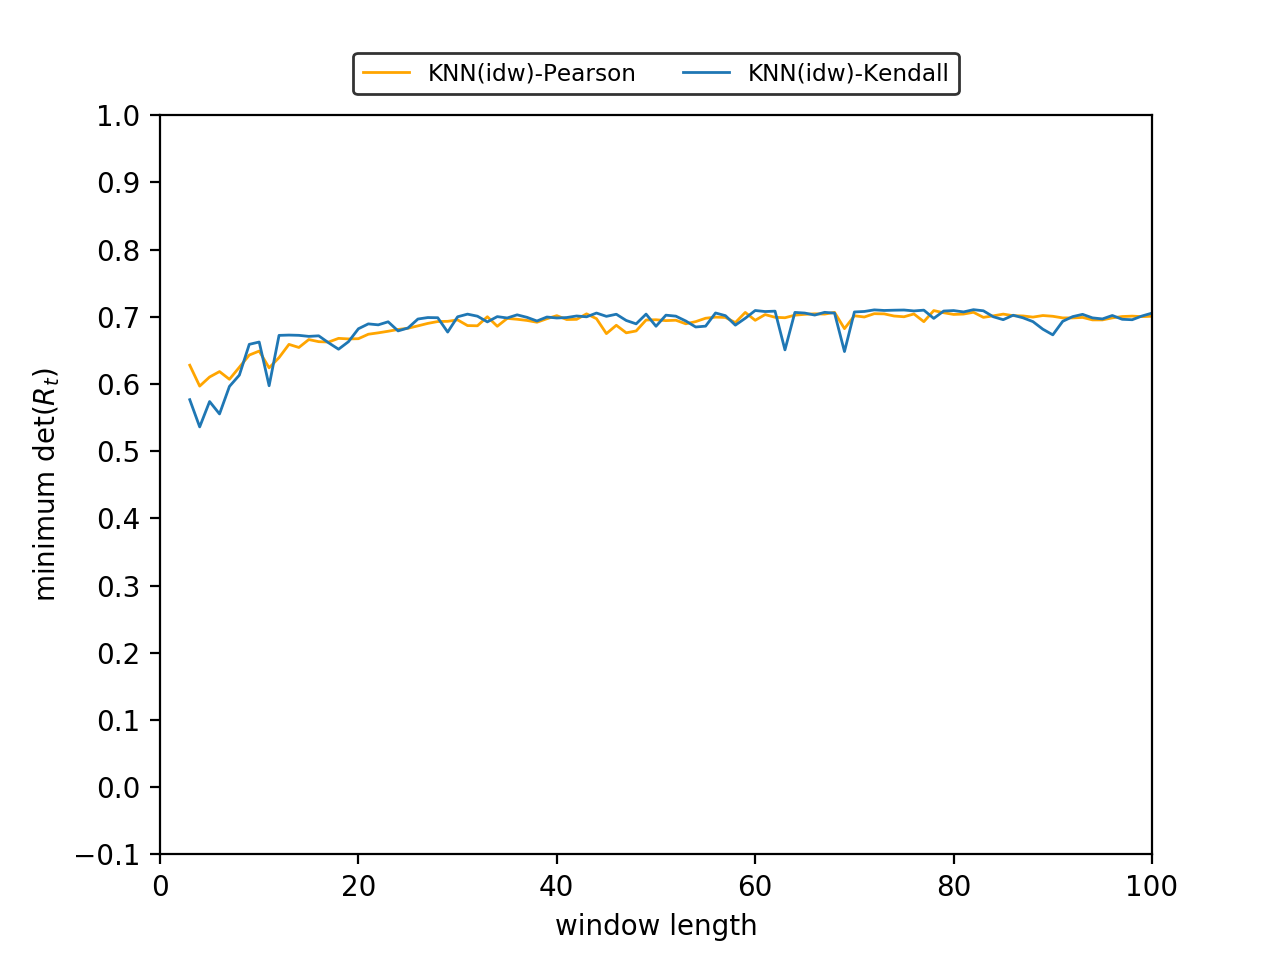
\includegraphics[width=\textwidth]{det_knn_IDW_pearson_kendall_true.png} 
		\caption{Minimum determinants for KNN estimates constructed from inverse distance weighting function, Pearson and Kendall covariates and true correlation.}
		\label{fig:det_knn_IDW_pearson_kendall_true.png}
	\end{subfigure}
	\caption{Comparison MSE and minimum determinants for KNN with true correlation, Pearson and Kendall Moving Window bootstrap estimates.}
	\label{fig:mse_det_knn5_idw_pearson_kendall_true}
\end{figure}


%%%%%%% RANDOM FOREST TRUE COR %%%%%%%%%%%%%%
\subsection{Generalization Error of Random Forest under True Correlation} \label{sec:MSE_rf_true}
The accuracy of RF estimates with Pearson and Kendall covariates for conditional correlation is compared by using the MSE between estimated and actual correlations. MSE from RF with Pearson and Kendall moving window estimates of correlation for covariates are shown in Fig. \ref{fig:mse_rf10_pearson_kendall_true}. Regardless of the choice of window length, MSE from RF with Pearson and Kendall covariates are between 0.0847 and 0.0980, and 0.0830 and 0.0983, respectively. The variance of MSE from RF estimates with Pearson covariates is approximately 8.42e-6 while that of RF estimates with Kendall covariates is approximately 8.92e-6. Analogous to KNN estimates of correlation, RF thus appears to be rather insensitive to the choice of window length, regardless whether the set of covariates is constructed from Pearson or Kendall moving window estimates of correlation. Moreover, RF estimates of conditional correlation satisfy the positive definiteness condition in the conditional correlation matrix $R_t$ for all time $t$ under all considered choices of window length. Fig. \ref{fig:det_rf10_pearson_kendall_true} presents the obtained minimum determinants of $R_t$ for all choices of window length.   

\begin{figure}[H]
	\centering
	\begin{subfigure}[b]{0.49 \textwidth} 
		\centering
		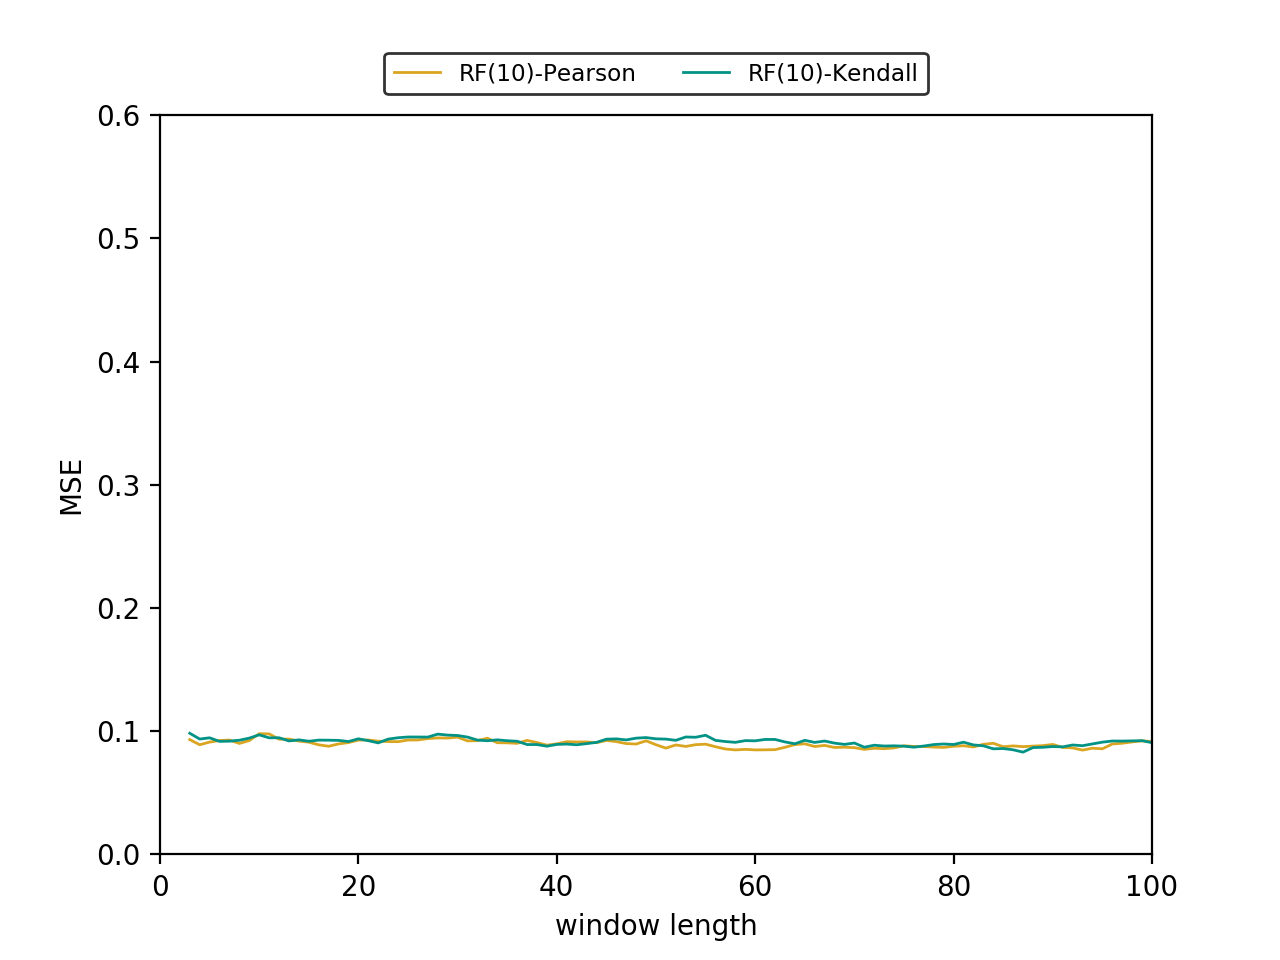
\includegraphics[width=\textwidth]{mse_rf10_pearson_kendall_true}
		\caption{MSE for RF with covariates from Pearson and Kendall and true correlation.}
		\label{fig:mse_rf10_pearson_kendall_true}
	\end{subfigure}
	\hfill
	\begin{subfigure}[b]{0.49 \textwidth} 
		\centering
		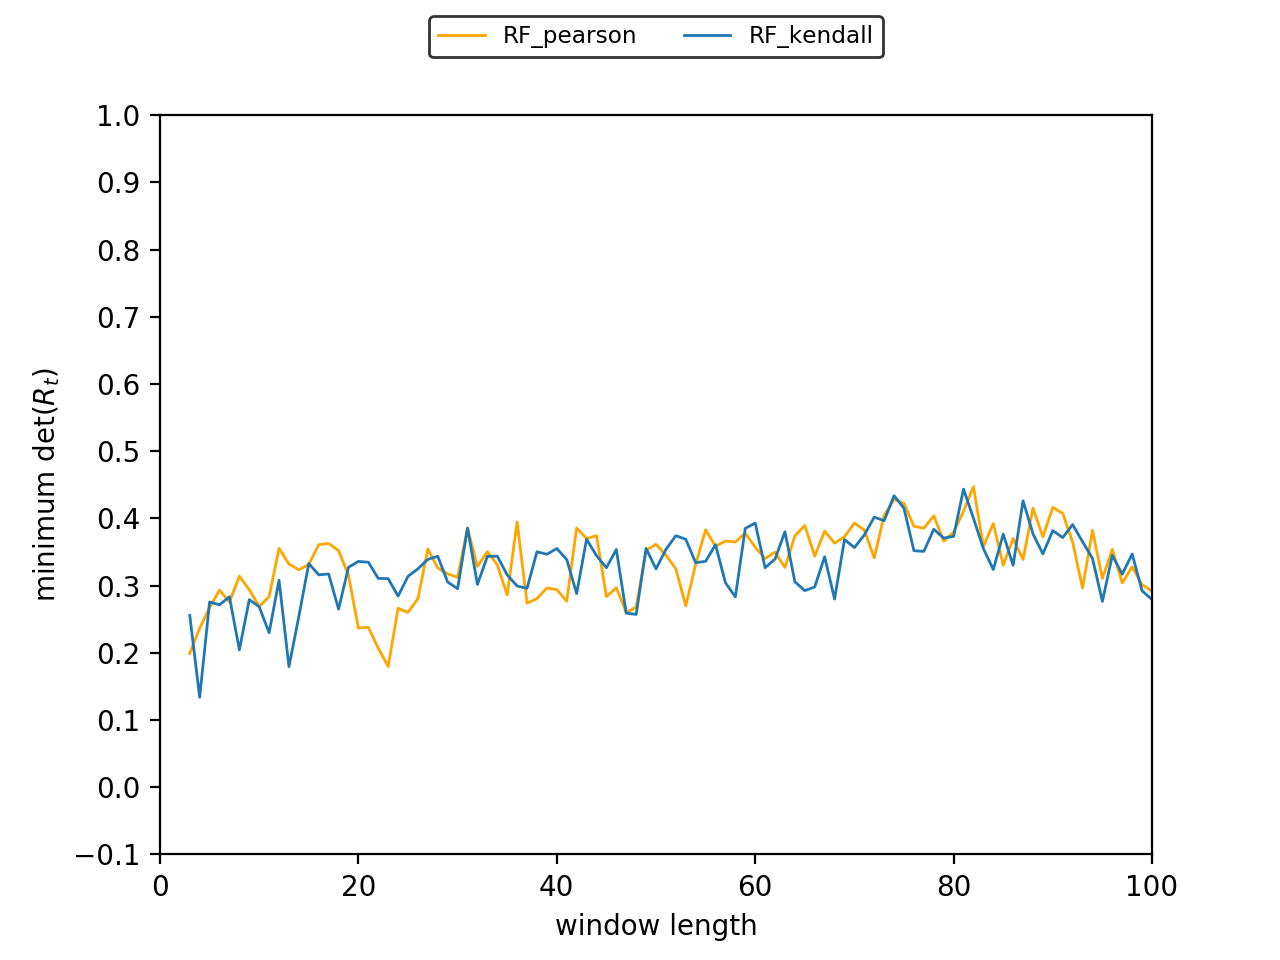
\includegraphics[width=\textwidth]{det_rf10_pearson_kendall_true}
		\caption{Minimum determinants for RF with covariates from Pearson and Kendall and true correlation.}
		\label{fig:det_rf10_pearson_kendall_true}
	\end{subfigure}
	\caption{Comparison MSE and minimum determinants for RF(n\_estimators=10) with covariates from Pearson and Kendall and true correlation.}
	\label{fig:mse_det_rf10_pearson_kendall_true}
\end{figure}

\noindent
From visual inspection of the plots in Fig. \ref{fig:rf_pearson21_bootstrap_true} and Fig. \ref{fig:rf_kendall21_bootstrap_true} it seems that the uncertainty in the conditional correlation, $\rho_t$, which is illustrated by the 99\% confidence interval, seems smaller for RF estimates compared to Pearson and Kendall moving window estimates under the same window length of 21. Analogous to KNN estimates of correlation, RF estimates of correlation under default parametrization, that is with number of trees in the decision forest equal to 10, are much more volatile than Pearson and Kendall sample correlations using moving windows. This may be a less desirable result as it is not expected that correlation between assets changes that drastically at each time unit. Rather, correlation is expected to vary gradually over time \citep{ref:Basturk2016} \\

\noindent
The MSE decomposition into bias and variance terms from RF estimates of correlation are shown in Fig. \ref{fig:decom_mse_rf10_pearson_true} and Fig. \ref{fig:decom_mse_rf10_kendall_true}. These figures indicate that the RF estimator is considerably less sensitive to the choice of the window length for smaller window sizes when compared to Pearson and Kendall sample correlations using moving windows depicted in Fig \ref{fig:mse_pearson_kendall_bootstrap}. The uncertainty around the estimated correlations appears to be marginally affected by the choice of the window length for all window sizes. This statement is supported by the fact that the variance as a function of the window length behaves like a (more or less) constant red line in these figures; a result analogous to conditional correlations obtained from the KNN estimator.


\begin{figure}[H]  % [h] parameter makes sure figures are located at 'this' location.
	\centering
	\begin{subfigure}[b]{0.49 \textwidth} % sum of widths should be less than text width if all one the same line
		\centering 
		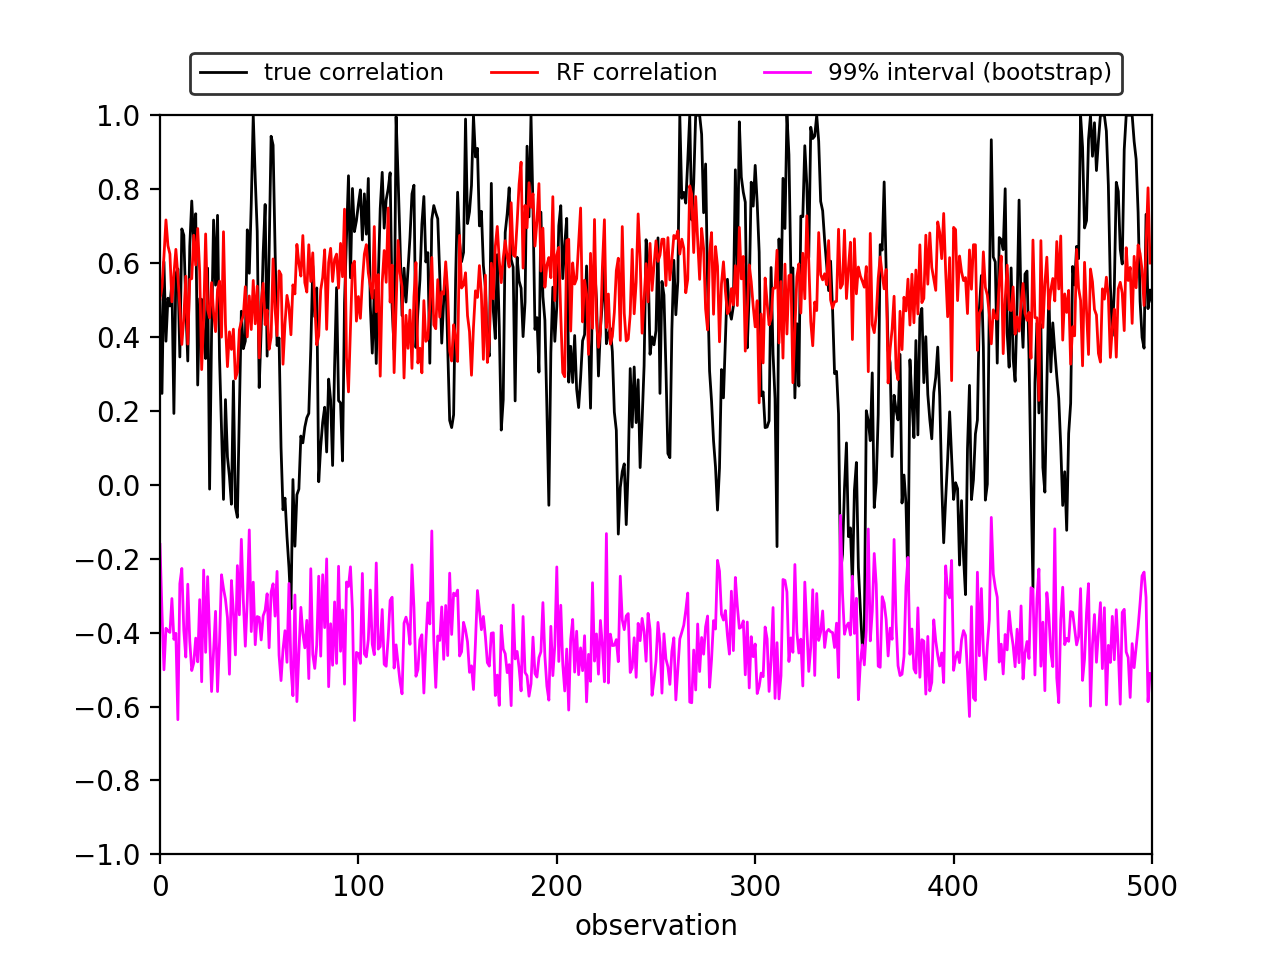
\includegraphics[width=\textwidth]{rf_pearson_21_estimates_bootstrap_true.png} 
		\caption{RF estimates with window size 21, Pearson as covariate and true correlation.} 	
		\label{fig:rf_pearson21_bootstrap_true}
	\end{subfigure} 
	\hfill	
	\begin{subfigure}[b]{0.49 \textwidth} 
		\centering 
		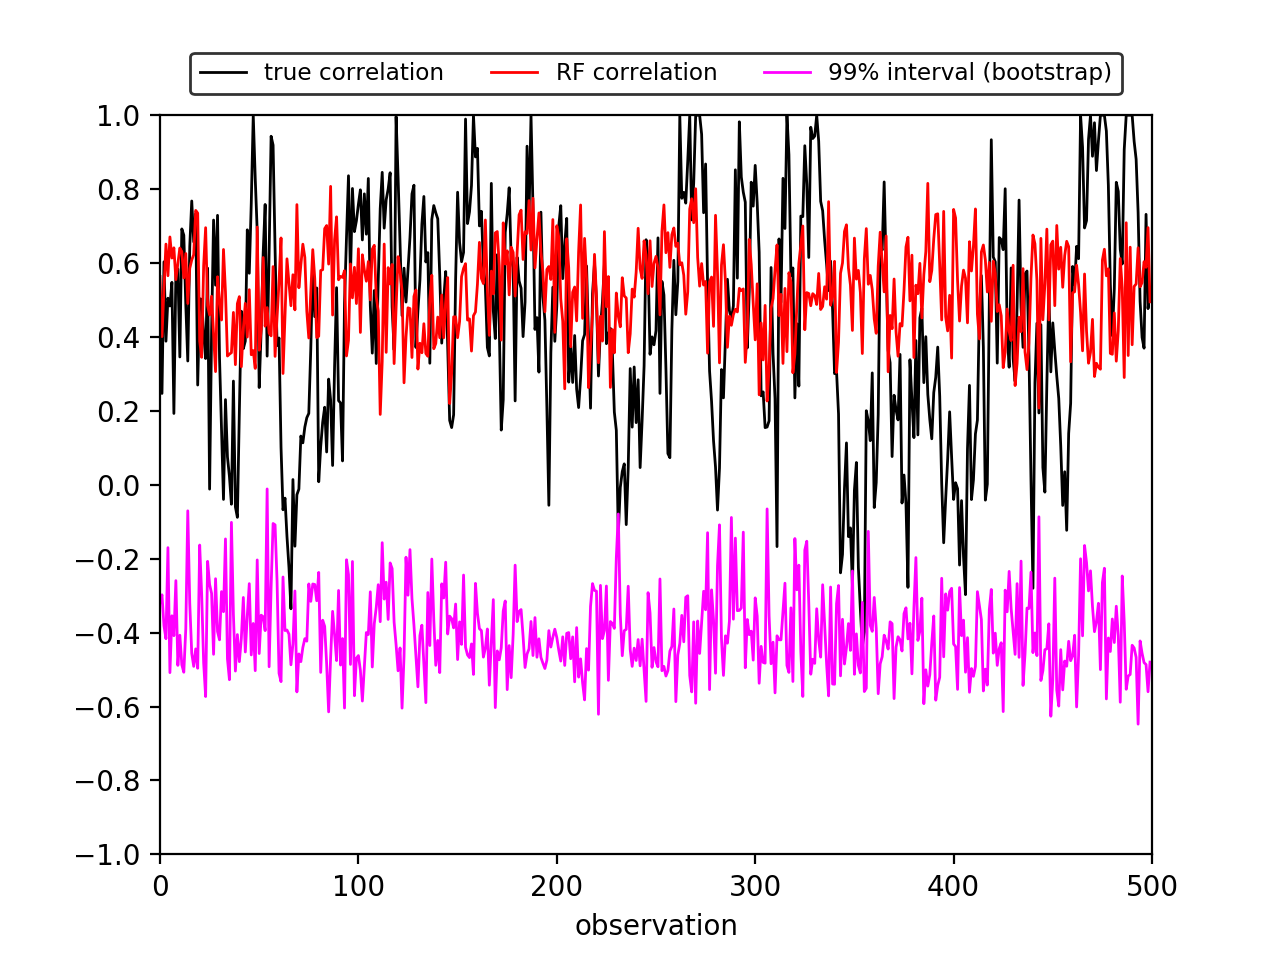
\includegraphics[width=\textwidth]{rf_kendall_21_estimates_bootstrap_true.png} 
		\caption{RF estimates with window size 21, Kendall as covariate and true correlation.} 
		\label{fig:rf_kendall21_bootstrap_true}
	\end{subfigure} 
	\hfill	
	\begin{subfigure}[b]{0.49 \textwidth}
		\centering 		
		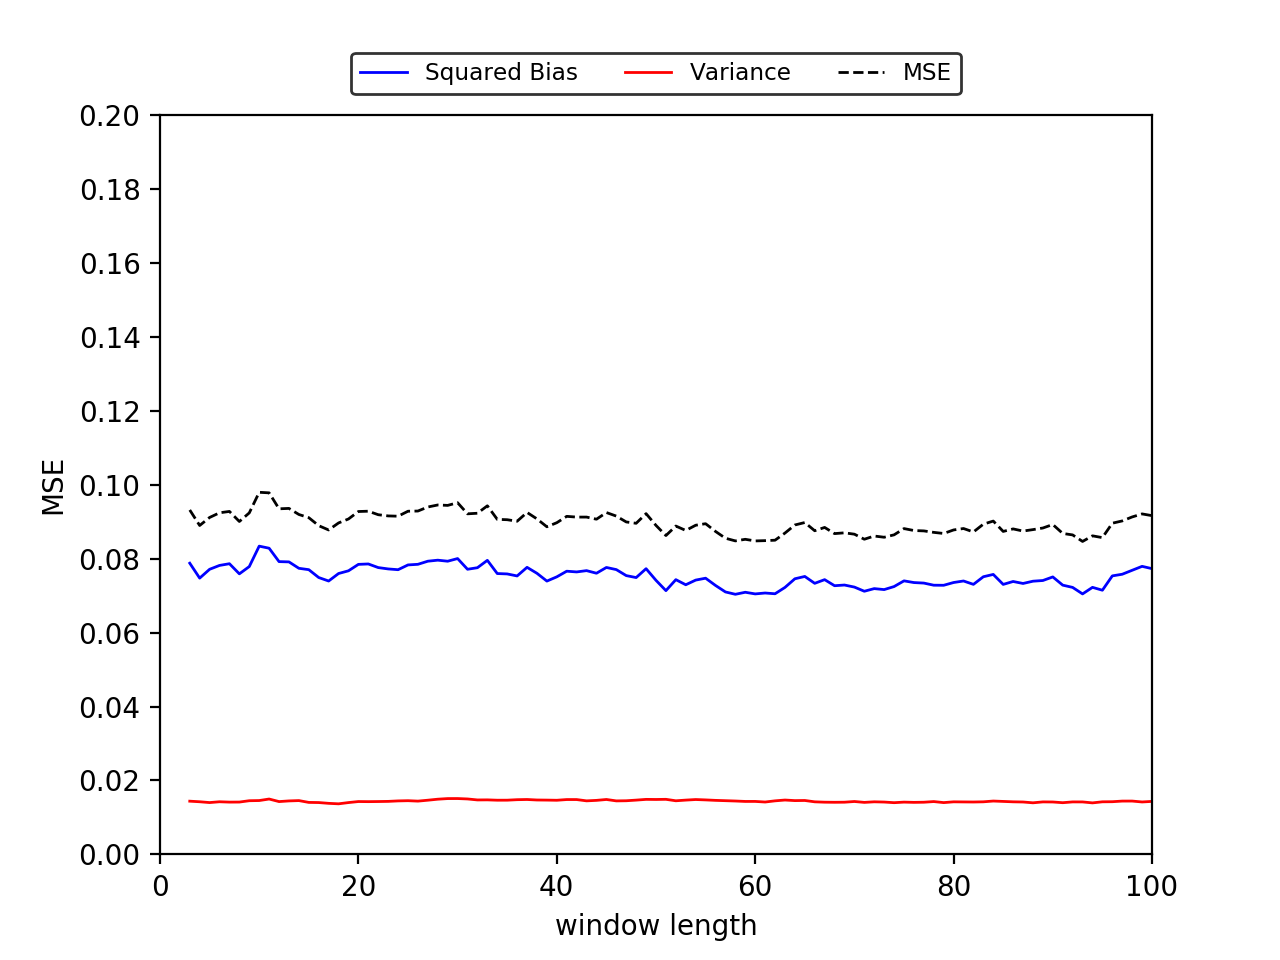
\includegraphics[width=\textwidth]{decom_mse_rf10_pearson_true.png} 
		\caption{Bias-variance decomposition for RF estimates with Pearson as covariate and true correlation.} 
		\label{fig:decom_mse_rf10_pearson_true}
	\end{subfigure}
	\hfill  
	\begin{subfigure}[b]{0.49 \textwidth}
		\centering 
		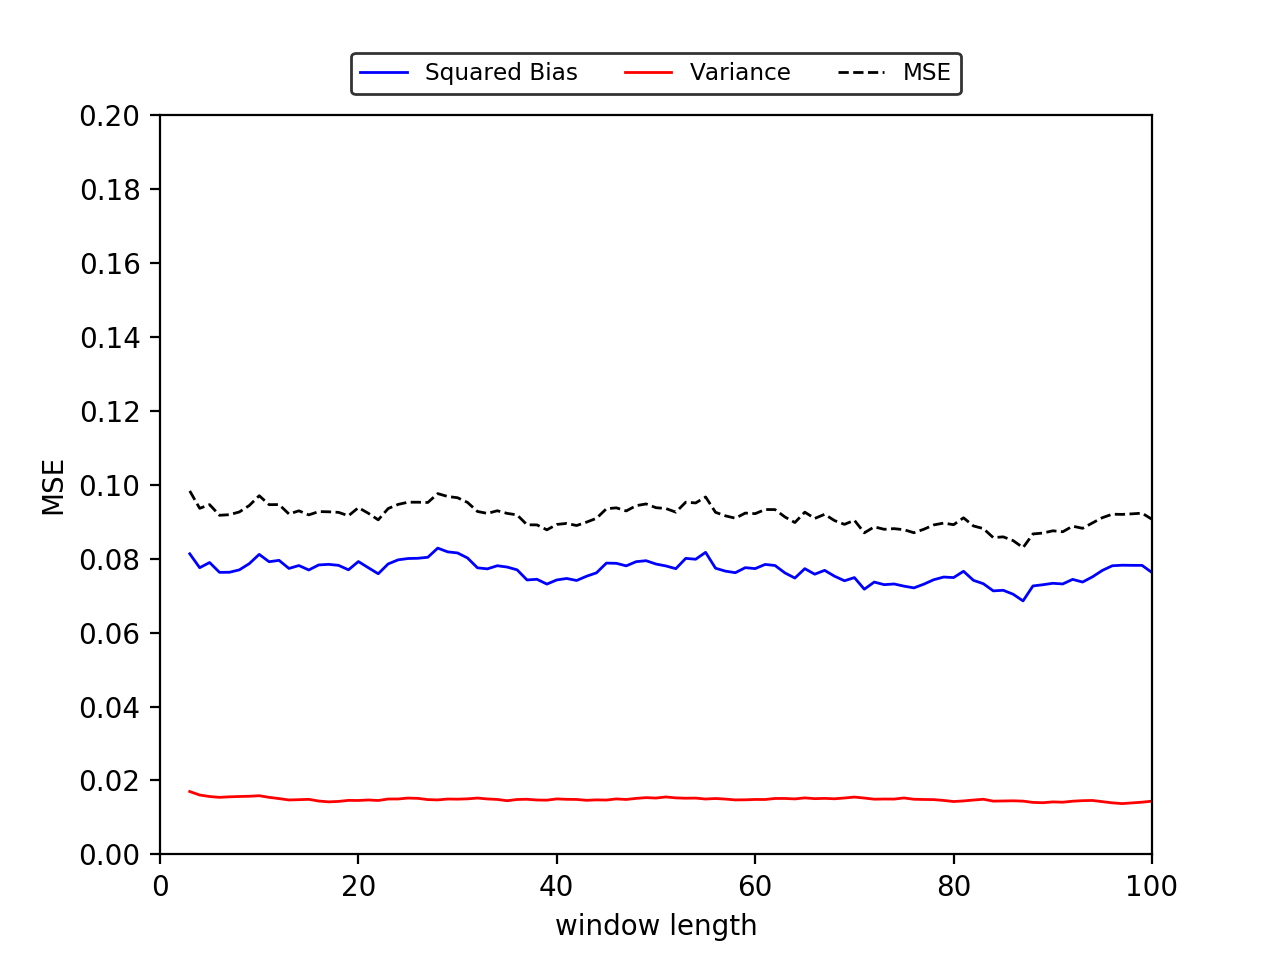
\includegraphics[width=\textwidth]{decom_mse_rf10_kendall_true.png} 
		\caption{Bias-variance decomposition for RF estimates with Kendall as covariate and true correlation.} 
		\label{fig:decom_mse_rf10_kendall_true}
	\end{subfigure}
	\caption{MSE for RF estimates with Pearson and Kendall Moving Window bootstrap estimates as covariates and true correlation.}
	\label{fig:decom_mse_rf10_pearson_kendall_true}
\end{figure}

\subsection{Effect of Alternative Random Forest Parameterizations under True Correlation} \label{sec:MSE_rf_alt_true}
Simulation results in Tabel \ref{tab:mse_decomp_rf_pearson_kendall_true}\footnote{Results were obtained by taking 100 bootstrapped samples instead of 1000 due to computational time constraints. This number of bootstrapped samples is however sufficient for illustrational purposes.} show an inverse relationship between the choice of the number of decision trees, or estimators, in the random forest and the uncertainty around the estimated correlations, regardless whether Pearson or Kendall estimates are used for specification of the set of covariates. It is clearly observed that an increase in the number of estimators results in a decrease of the variance, and conversely. This observation is in line with our discussion on MSE decomposition for the RF estimator and Eq. \eqref{eq:variance_rf} in Section \ref{sec:mse_decompose}. For this particular data set it is observed that the point of diminishing reduction in variance is reached around 300 decision trees. An increase in number of decision trees after that does not significantly reduce the variance. \\  

\noindent
With respect to our discussion on the effect of random covariate selection in individual tree construction on the squared bias and variance (for reference, see Section \ref{sec:mse_decompose}: the individual decision trees of the random forest in our simulation are merely decision stumps as the dimension of the covariate set is only three (minimum and maximum returns and pairwise correlation of the previous time unit), $P=3$, which means under default randomization for regression problems $p=P/3 = 1$. As such, no sensitivity analysis is done on the number of covariates given the small dimension of the covariate set. This might, however, may be interesting in case of high dimensional correlation systems. \\  


%% TABLE
\begin{table}[H]
\centering
\captionsetup[subtable]{position=below}
%\captionsetup[table]{position=below}
\begin{subtable}{0.49\linewidth}
\centering
\begin{tabular}{r  c  c  c} 
\toprule
\multicolumn{1}{ r }{\textbf{Trees}} &
\multicolumn{1}{ c }{\textbf{Squared Bias}} &
\multicolumn{1}{ c }{\textbf{Variance}} &
\multicolumn{1}{ c }{\textbf{MSE}} \\
\midrule 

10                                   &   0.0839                       & 0.0144                & 0.0983      \\
100                                 & 0.0839                         & 0.0077               & 0.0916       \\
300                                 & 0.0837                         & 0.0071               & 0.0908      \\
600                                 & 0.0841                         & 0.0070               & 0.0911     \\
1000                               & 0.0837                         &  0.0069              & 0.0906     \\ [1ex]

\bottomrule
\end{tabular}
\caption{MSE for RF estimates with window size 10, Pearson as covariate and true correlation.}
\label{tab:mse_decomp_rf_pearson_true}
\end{subtable}
\hfill
\begin{subtable}{0.49\linewidth}
\centering
\begin{tabular}{r  c  c  c} 
\toprule
\multicolumn{1}{ r }{\textbf{Trees}} &
\multicolumn{1}{ c }{\textbf{Squared Bias}} &
\multicolumn{1}{ c }{\textbf{Variance}} &
\multicolumn{1}{ c }{\textbf{MSE}} \\
\midrule 

10                                   & 0.0817                         & 0.0158               &  0.0976     \\
100                                 & 0.0815                         & 0.0088               & 0.0903      \\
300                                 & 0.0813                         & 0.0082               & 0.0895      \\
600                                 & 0.0817                         & 0.0082               & 0.090     \\
1000                               &  0.0814                         &  0.0080             & 0.0894     \\ [1ex]

\bottomrule
\end{tabular}
\caption{MSE for RF estimates with window size 10, Kendall as covariate and true correlation.}
\label{tab:mse_decomp_rf_kendall_true}
\end{subtable}
\caption{Mean Squared Error (MSE) decomposition as a function of the number of estimators (trees) for RF with proxy for covariates and true correlation.}
\label{tab:mse_decomp_rf_pearson_kendall_true}
\end{table}

\noindent
This section is concluded with a comparison of the function approximation capabilities of the RF estimator and Pearson and Kendall sample correlation estimates using moving windows. Comparison is based on MSE between estimated and actual correlations. Fig. \ref{fig:mse_rf10_pearson_kendall_comp_true.png} shows MSE from RF under default parameterization where the number of estimators equals 10, as well as Pearson and Kendall moving window estimates of conditional correlations. According to MSE, default parameterizations of the RF estimator where the random forest is constructed from 10 decision trees yields significantly smaller MSE compared to Pearson and Kendall sample correlation estimates using moving windows for all window sizes. Finally, the variance of MSE from RF estimates under default parameterizations and Pearson and Kendall approximations of true correlation in Fig. \ref{fig:mse_rf10_pearson_kendall_comp_true.png} are 8.42e-6 and 8.92e-6, respectively, while that of Pearson and Kendall moving window estimates are 0.0040 and 0.0037, respectively. \\


\begin{figure}[H]
	\centering
	\begin{subfigure}[b]{0.49 \textwidth} 
		\centering
		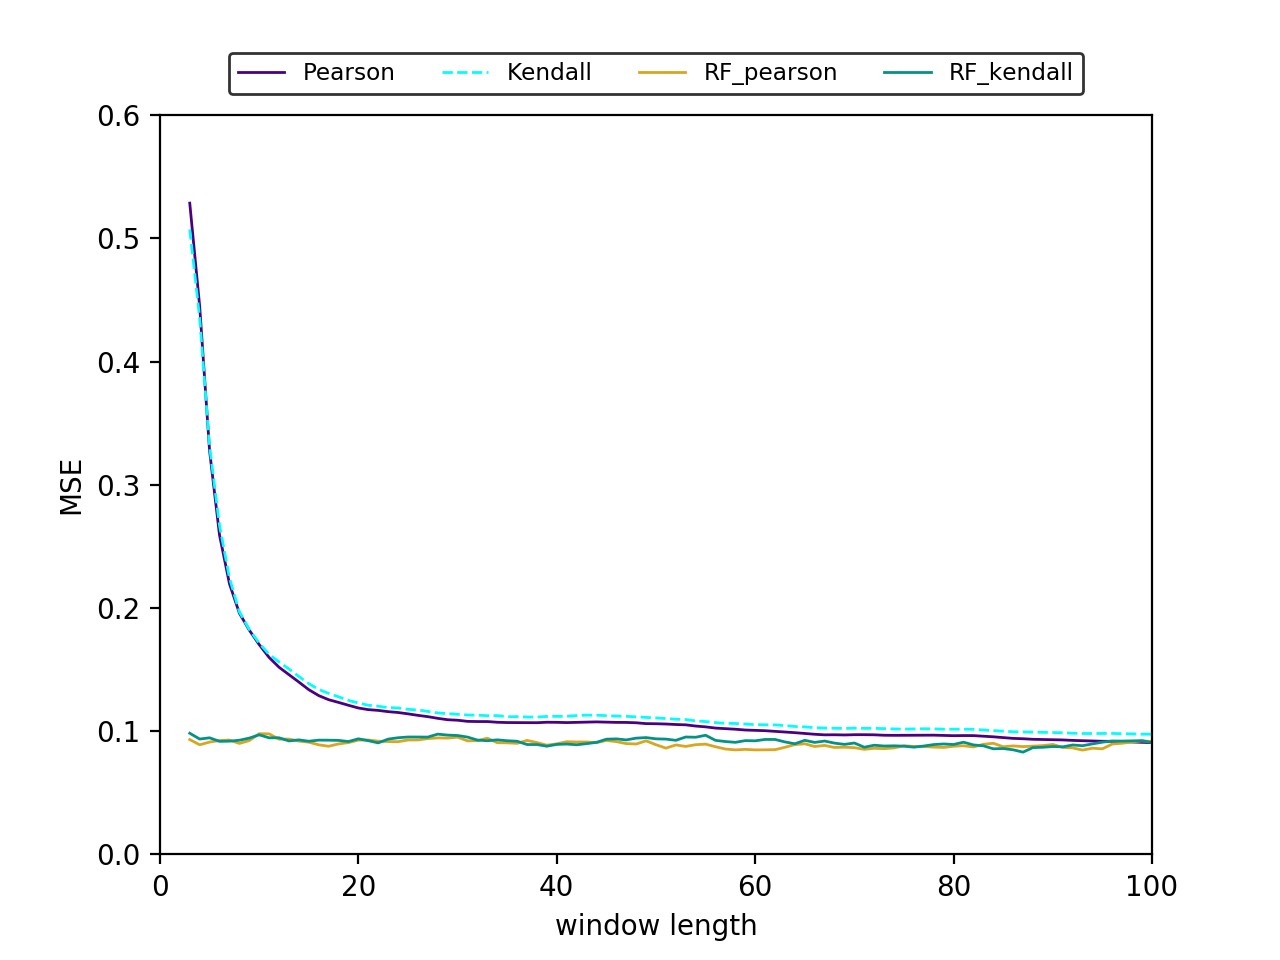
\includegraphics[width=\textwidth]{mse_rf10_pearson_kendall_comp_true.png}
		%\caption{MSE for RF with covariates from Pearson and Kendall and true correlation.}
		%\label{fig:mse_rf10_pearson_kendall_comp_true.png}
	\end{subfigure}
	\caption{Comparison MSE for RF(n\_estimators=10) with true correlation, Pearson and Kendall Moving Window bootstrap estimates.}
	\label{fig:mse_rf10_pearson_kendall_comp_true.png}
\end{figure}

\noindent
\textbf{Potentially add RF(n\_estimators=100) to show that this parameterization performs even better due to variance reduction. Maybe mentioning this with reference to the sensitivity analysis is also sufficient.}


%%%%%%%%%%%%%%%%%%%%%%%%%%%%%%%%%%%%%
%%%%%%%%%% Proxies for Correlation %%%%%%%%%%%%%%%%
%%%%%%%%%%%%%%%%%%%%%%%%%%%%%%%%%%%%%%
\section{Learning with Proxy for Response Variable} \label{sec:proxy_correlation}
This section is premised on a more realistic approach to apply nearest neighbor and random forest as estimators of conditional correlation. Both the covariates and response variable are obtained from Pearson or Kendall sample estimates using moving windows, as defined in \eqref{eq:mw_rho} and \eqref{eq:mw_kendall}, respectively. This is different from Section \ref{sec:true_correlation} where the response variable of the learning estimators was defined as the true observed correlation (given by the simulated parameters). This setup allows us to study the effect of using approximations of correlations for both covariates and response variable on the loss function. \\

%%%%%% NEAREST NEIGHBOR PROXY 	%%%%%%%%
\subsection{Generalization Error of Nearest Neighbor under Proxy Correlation} \label{sec:MSE_knn_proxy}
The accuracy of KNN estimates with Pearson and Kendall sample correlation estimates using moving windows for both covariates and response variable is compared by using mean squared error (MSE) between estimated and actual correlations. MSE from KNN with Pearson and Kendall moving window estimates of correlation is shown in Fig. \ref{fig:mse_knn5_pearson_kendall_proxy}. Regardless of the choice of window length, MSE from KNN with Pearson and Kendall covariates are between 0.0855 and 0.2555, and 0.0952 and 0.2223, respectively. The variance of MSE from KNN estimates with Pearson covariates is approximately 5.70e-4 while that of KNN estimates with Kendall covariates is approximately 2.96e-4. Recall that in Fig. \ref{fig:mse_knn5_pearson_kendall_true} the KNN estimator appeared to be insensitive to the choice of window length when the response variable is specified by the true correlation. Interestingly, Fig. \ref{fig:mse_knn5_pearson_kendall_proxy} shows that MSE from KNN estimation with Pearson or Kendall approximations for the response variable varies substantially for smaller window sizes. Although, less variation is observed when compared with MSE from Pearson and Kendall moving window estimates depicted in Fig. \ref{fig:mse_pearson_kendall_bootstrap}. Moreover, KNN estimates of conditional correlation with both the set of covariates and response variable approximations of true correlation satisfy the positive definiteness condition in the conditional correlation matrix $R_t$ for all time $t$ under all choices of window length. Fig. \ref{fig:det_knn5_pearson_kendall_proxy} presents the obtained minimum determinants of $R_t$ for all choices of window length.  
     
\begin{figure}[H]
	\centering
	\begin{subfigure}[b]{0.49 \textwidth} 
		\centering
		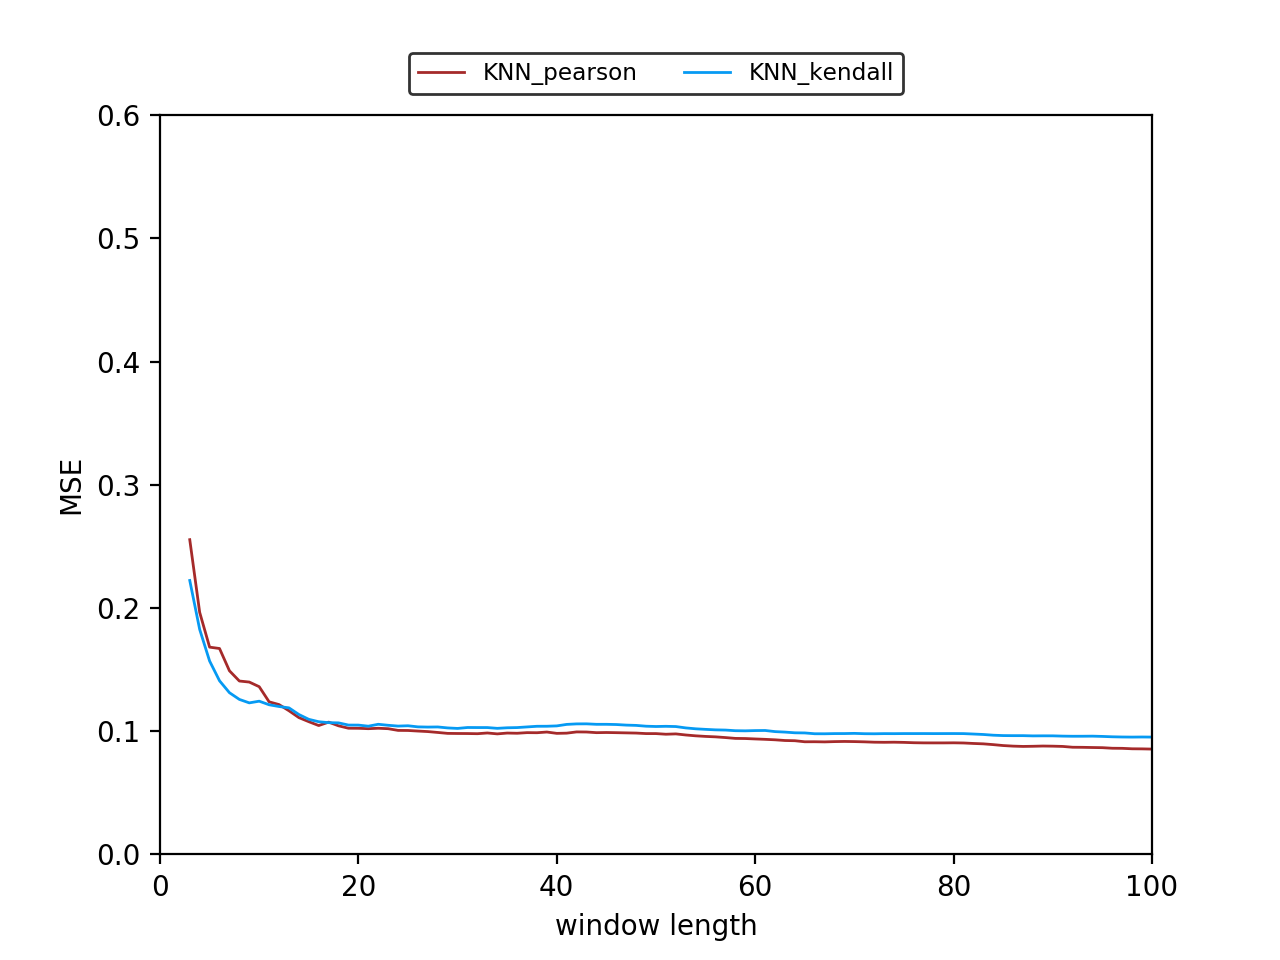
\includegraphics[width=\textwidth]{mse_knn5_pearson_kendall_proxy.png}
		\caption{MSE for KNN with covariates from Pearson and Kendall and proxy correlation.}
		\label{fig:mse_knn5_pearson_kendall_proxy}
	\end{subfigure}
	\hfill
	\begin{subfigure}[b]{0.49 \textwidth} 
		\centering
		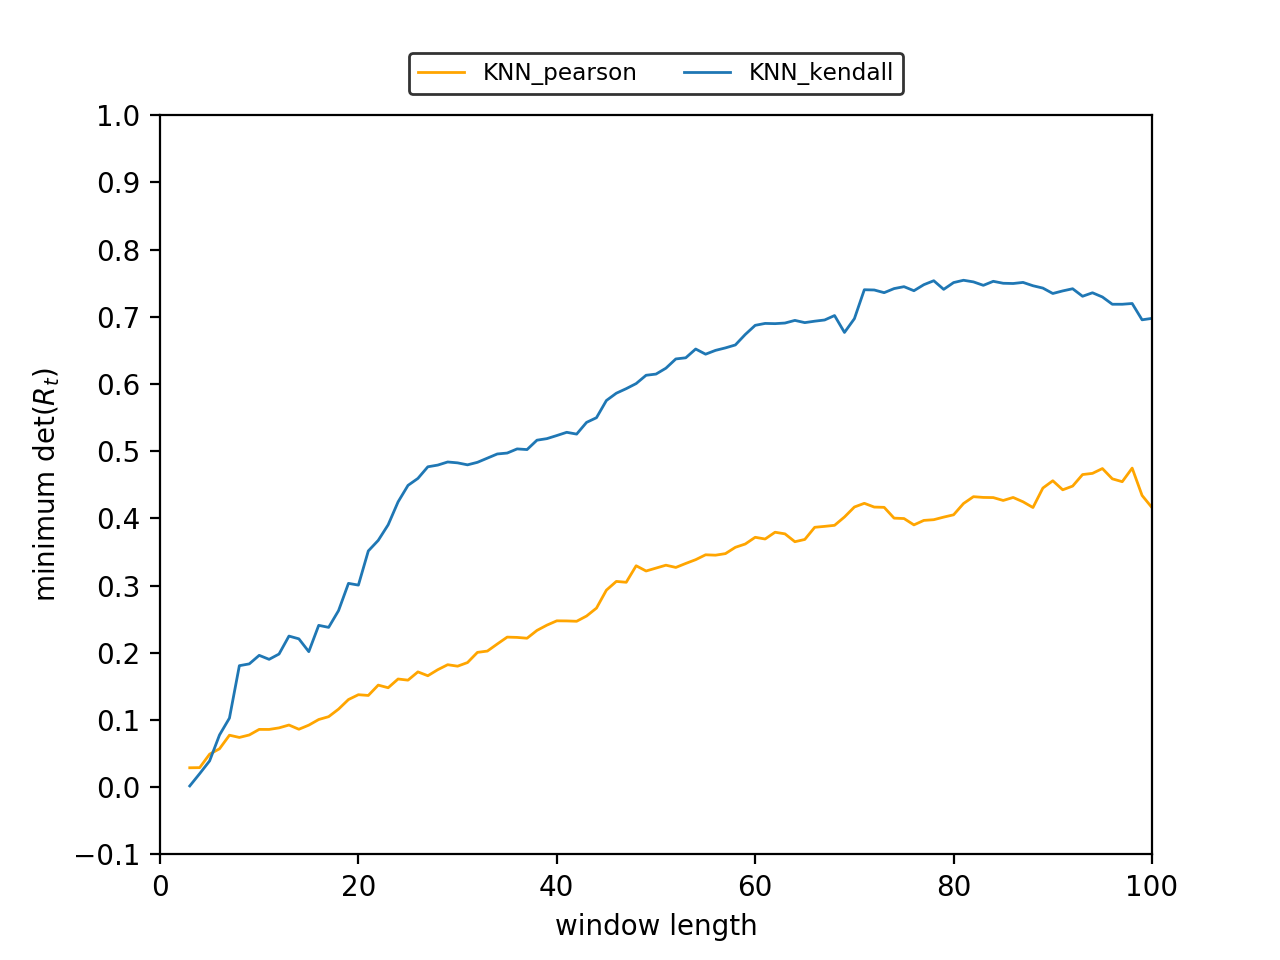
\includegraphics[width=\textwidth]{det_knn5_pearson_kendall_proxy}
		\caption{Minimum determinants for KNN with covariates from Pearson and Kendall and proxy correlation.}
		\label{fig:det_knn5_pearson_kendall_proxy}
	\end{subfigure}	
	\caption{Comparison MSE and minimum determinants for KNN(n\_neighbors=5) with covariates from Pearson and Kendall and proxy correlation.}
	\label{fig:mse_det_knn5_pearson_kendall_proxy}
\end{figure}

\noindent
From visual inspection of the plots in Fig. \ref{fig:knn_pearson21_bootstrap_proxy} and Fig. \ref{fig:knn_kendall21_bootstrap_proxy} it is clear that the uncertainty in the conditional correlation, $\rho_t$, 
which is illustrated by the $99\%$ confidence interval, is smaller for KNN estimates compared to Pearson moving window estimates and Kendall moving window estimates, even though both the set of covariates and the response variable of the KNN algorithm are based on approximations of correlation instead of actual correlation. These figures also show smaller uncertainty in the conditional correlation $\rho_t$ when compared with KNN estimates with true correlation as the response variable, which are depicted in Fig. \ref{fig:decom_mse_knn5_pearson_kendall_proxy}. Moreover, KNN estimates of correlation with true correlation as response variable in Fig. \ref{fig:knn_pearson21_bootstrap_proxy} and Fig. \ref{fig:knn_kendall21_bootstrap_proxy} are much more volatile. KNN estimates with approximated correlation as response variable in Fig. \ref{fig:knn_pearson21_bootstrap_proxy} and Fig. \ref{fig:knn_kendall21_bootstrap_proxy}, however, follow the increases and decreases of the actual correlation smoother, with tighter confidence intervals. This is a more desirable result as it is not expected that correlation between assets changes that drastically at each time unit.  \\


\noindent
The MSE decomposition into bias and variance terms from KNN estimates of correlation are shown in Fig. \ref{fig:decom_mse_knn_pearson_proxy} and Fig. \ref{fig:decom_mse_knn_kendall_proxy}. These figures indicate that the KNN estimator with approximated response variable is more sensitive to the choice of the window length for smaller window sizes compared to the KNN estimator with true correlation depicted in Fig. \ref{fig:decom_mse_knn5_pearson_kendall_true}. This observation can be explained by error propagation: the effect of covariates' uncertainties (or errors) on the error of the function based on them. In the case when the KNN estimator uses approximated response variable for learning, the error associated with approximation of true correlation using moving window estimates is propagated to the response of the KNN estimator. Fig. \ref{fig:decom_mse_knn_pearson_proxy} and Fig. \ref{fig:decom_mse_knn_kendall_proxy} show, however, that the KNN estimator with approximated response variable is considerably less sensitive to the choice of the window length for smaller window sizes when compared to Pearson and Kendall sample correlation estimates using moving windows depicted in Fig. \ref{fig:decom_mse_pearson} and Fig \ref{fig:decom_mse_kendall}, respectively. The KNN estimator thus seems to mitigate the error propagation to some extend for smaller window sizes. This may be explained by the fact that KNN estimator, even with a small number of neighbors such as under the default parameterization where $k=5$, uses neighbors that contain additional informational value compared to the informational value in moving window estimates with small window sizes.      


\begin{figure}[H]  % [h] parameter makes sure figures are located at 'this' location.
	\centering
	\begin{subfigure}[b]{0.49 \textwidth} % sum of widths should be less than text width if all one the same line
		\centering 
		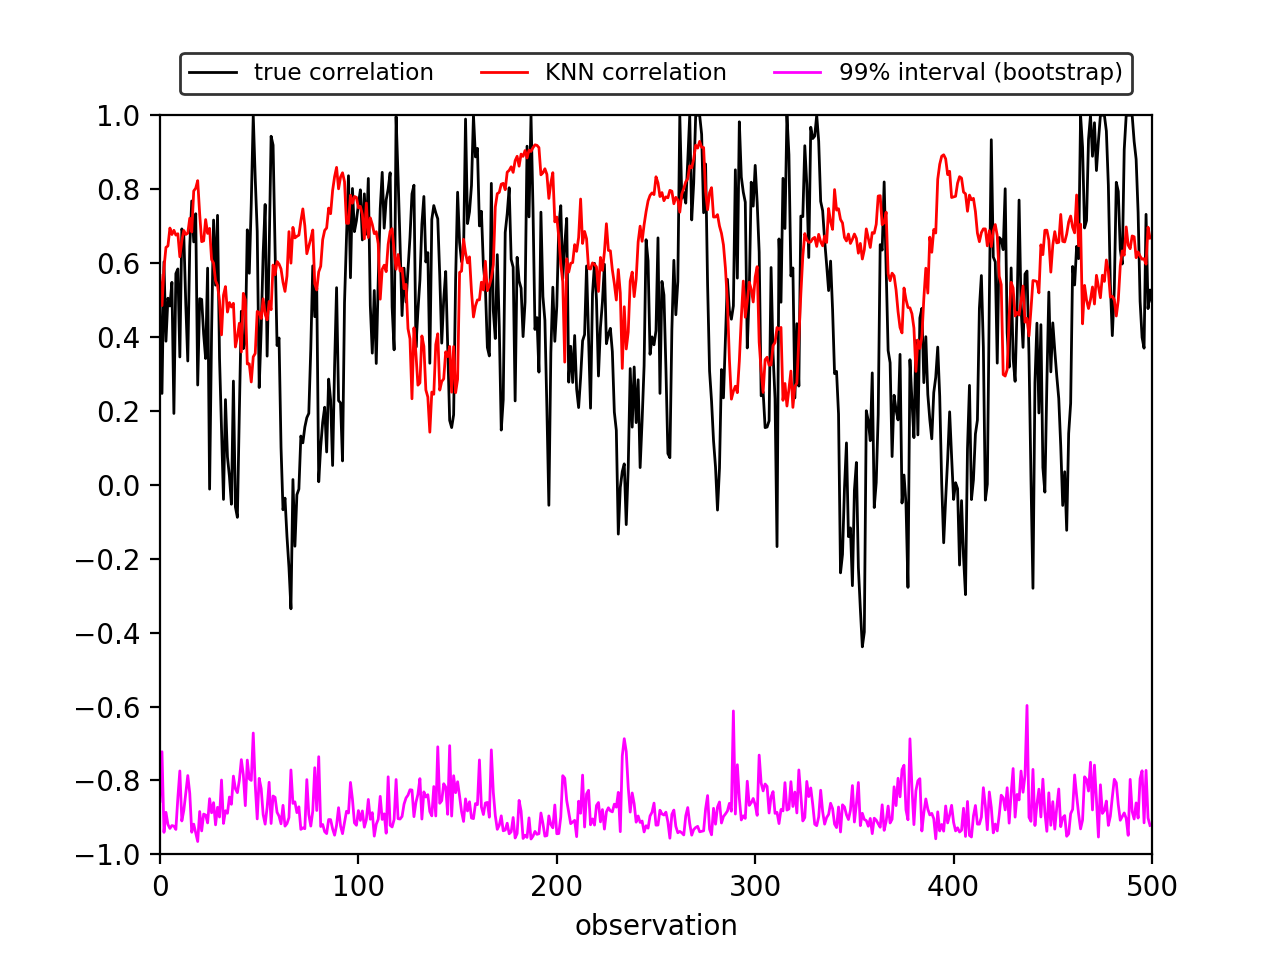
\includegraphics[width=\textwidth]{knn_pearson_21_estimates_bootstrap_proxy.png} 
		\caption{KNN estimates with window size 21, Pearson as covariate and proxy correlation.} 	
		\label{fig:knn_pearson21_bootstrap_proxy}
	\end{subfigure} 
	\hfill	
	\begin{subfigure}[b]{0.49 \textwidth} 
		\centering 
		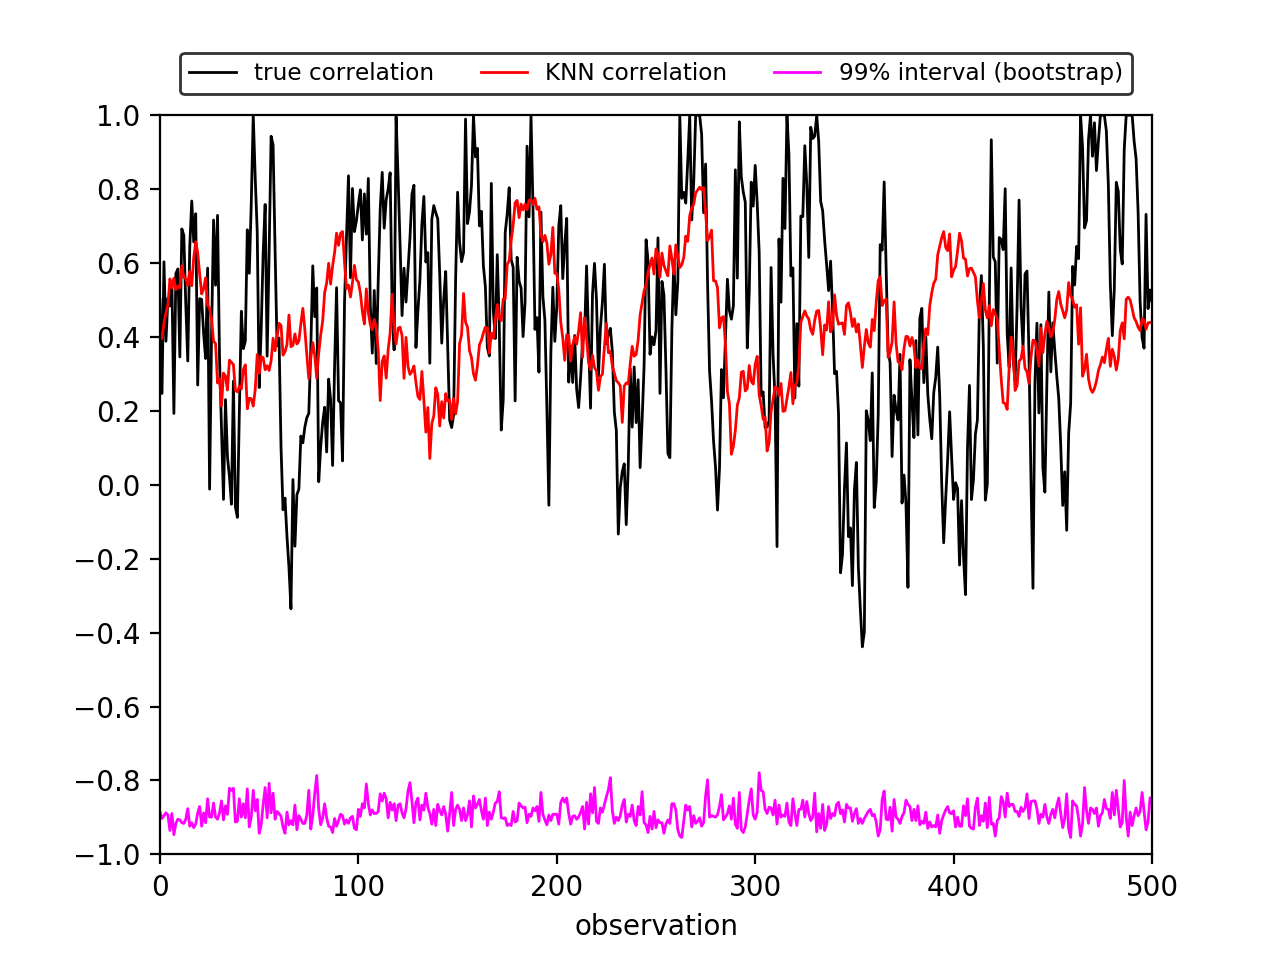
\includegraphics[width=\textwidth]{knn_kendall_21_estimates_bootstrap_proxy.png} 
		\caption{KNN estimates with window size 21, Kendall as covariate and proxy correlation.} 
		\label{fig:knn_kendall21_bootstrap_proxy}
	\end{subfigure} 
	\hfill	
	\begin{subfigure}[b]{0.49 \textwidth}
		\centering 
		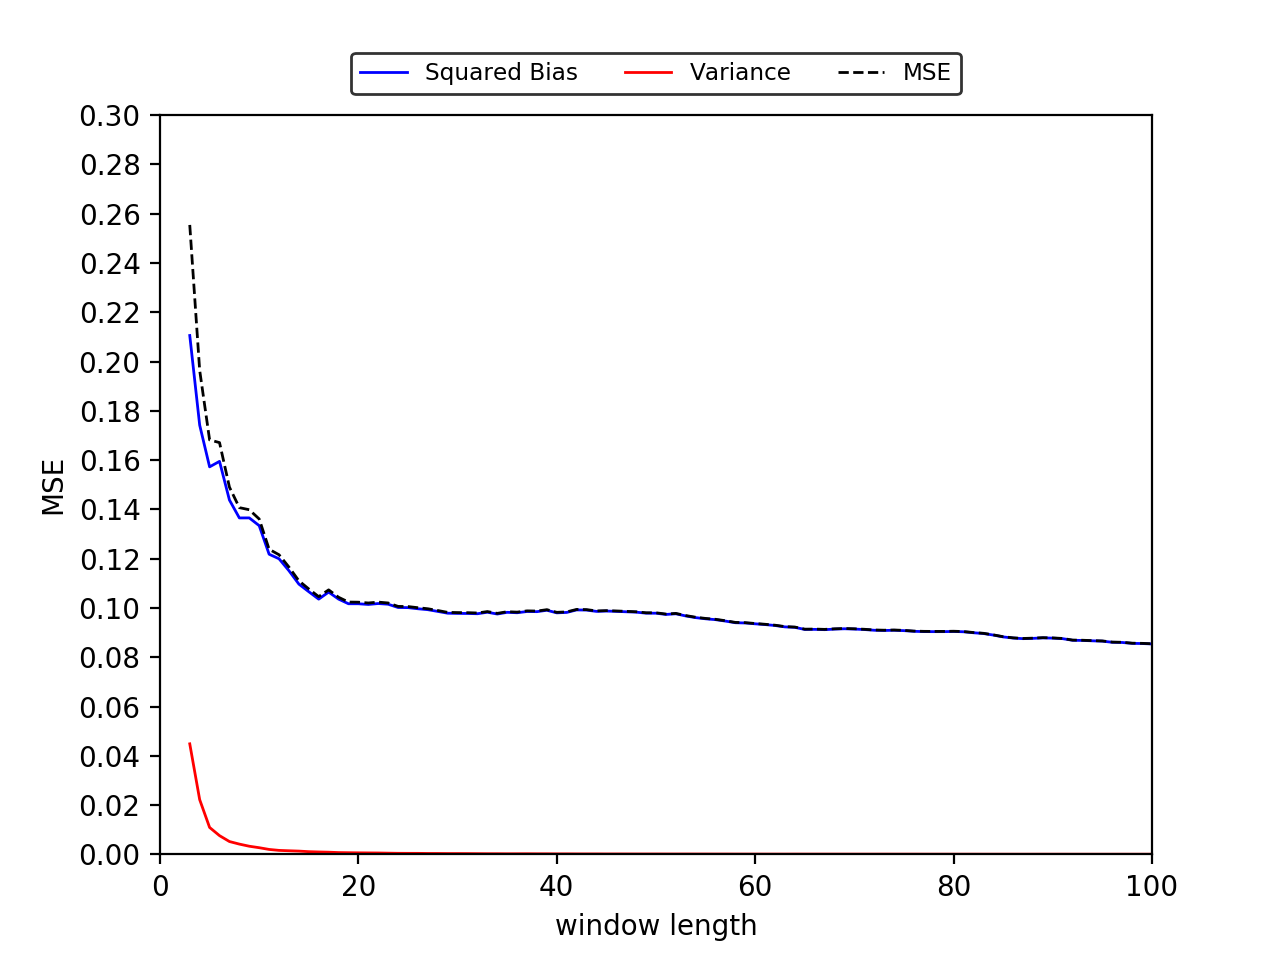
\includegraphics[width=\textwidth]{decom_mse_knn_pearson_proxy.png} 
		\caption{Bias-variance decomposition for KNN estimates with Pearson as covariate and proxy correlation.} 	
		\label{fig:decom_mse_knn_pearson_proxy}
	\end{subfigure}
	\hfill  
	\begin{subfigure}[b]{0.49 \textwidth}
		\centering 
		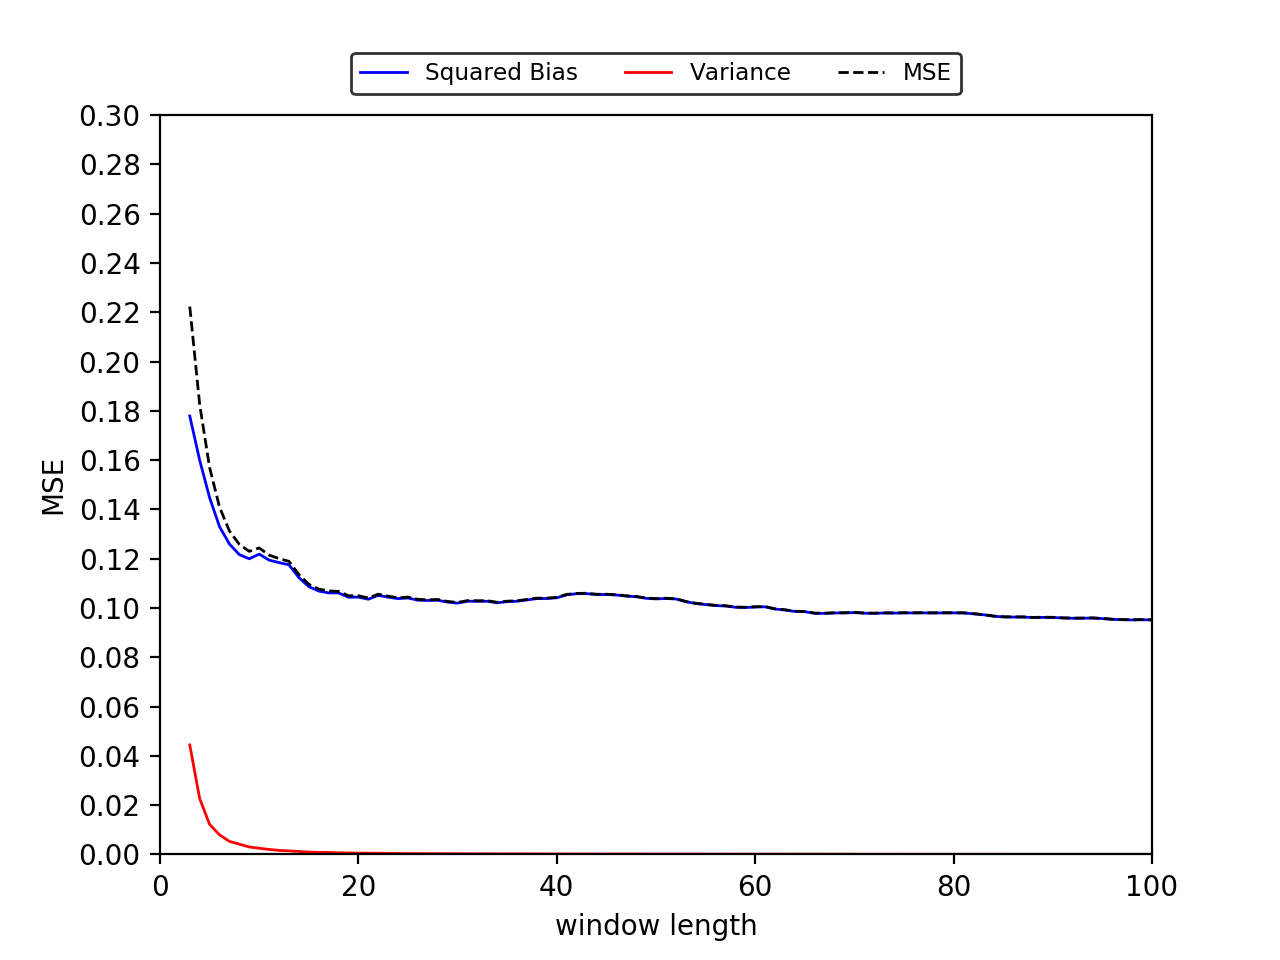
\includegraphics[width=\textwidth]{decom_mse_knn_kendall_proxy.png} 
		\caption{Bias-variance decomposition for KNN estimates with Kendall as covariate and proxy correlation.} 
		\label{fig:decom_mse_knn_kendall_proxy}
	\end{subfigure}
	\caption{MSE for KNN estimates with Pearson and Kendall Moving Window bootstrap estimates as covariates and proxy correlation.}
	\label{fig:decom_mse_knn5_pearson_kendall_proxy}
\end{figure}


\subsection{Effect of Alternative Nearest Neighbor Parameterizations under Proxy Correlation} \label{sec:MSE_knn_alt_proxy}
Tabel \ref{tab:mse_decomp_knn_pearson_kendall_proxy} presents MSE decomposition as a function of number of neighbors $k$ for KNN estimators with approximations for both covariates and response variable. Similar results are observed for $k \in \{5, 10, 25, 50, 100\}$ when compared with KNN estimators with approximated covariates and true correlation in Tabel \ref{tab:mse_decomp_knn_pearson_kendall_true}; both squared bias and variance decrease with an increase in $k$, and conversely, regardless whether the set of covariates is constructed from Pearson or Kendall correlation estimates using moving windows. Given Eq. \eqref{eq:mse_decomposition_knn} and our discussion from Section \ref{sec:mse_decompose}, one might have expected an increase in squared bias with an increase in $k$. A possible explanation for this behavior may be that up to some $k$, an increase in $k$ implies additional neighbors containing informational value are used for estimation of conditional correlation. Logically, the inclusion of additional neighbors containing informational value yields more accurate estimates of correlation, that is, a decrease in squared bias. As of some $k$, however, additional neighbors only add noise to the estimation process which results into increased squared bias. For KNN estimates with Kendall covariates and proxy correlation this is for $k = 900$ whereas squared bias still decreases for $k = 1000$ in the case of KNN estimates with Pearson covariate and proxy correlation. Given our discussion from Section \ref{sec:mse_decompose} and results from KNN estimators with approximated covariates and true correlation in Tabel \ref{tab:mse_decomp_knn_pearson_kendall_true}, one might have expected a continuing decrease in variance with an increase in $k$. Interestingly, Tabel \ref{tab:mse_decomp_knn_pearson_kendall_proxy} shows an increase in variance from $k = 800$ and $k = 900$ onwards for KNN estimates with Pearson and Kendall covariates, respectively.          


%% TABLE
\begin{table}[H]
\centering
\captionsetup[subtable]{position=below}
%\captionsetup[table]{position=below}
\begin{subtable}{0.49\linewidth}
\centering
\begin{tabular}{r  c  c  c} 
\toprule
\multicolumn{1}{ r }{\textbf{k}} &
\multicolumn{1}{ c }{\textbf{Squared Bias}} &
\multicolumn{1}{ c }{\textbf{Variance}} &
\multicolumn{1}{ c }{\textbf{MSE}} \\
\midrule 

5                                     & 0.1334                         & 0.0027                & 0.1361     \\
10                                   & 0.1319                         & 0.0015                & 0.1334     \\
25                                   & 0.1289 	                    & 6.64e-4                & 0.1295     \\
50                                   & 0.1268                         & 3.57e-4                & 0.1271     \\
100                                 & 0.1238                         & 1.95e-4               & 0.1240      \\
200                                 & 0.1169                         & 1.14e-4               & 0.1170      \\
400                                 & 0.1047                         & 7.80e-5               & 0.1048      \\
600                                 & 0.0946                         & 7.20e-5               & 0.0947     \\
800                                 & 0.0870                         & 7.50e-5               & 0.0870      \\
900				     & 0.0841			   & 8.00e-5              & 0.0842      \\
1000                               & 0.0827                         & 8.80e-5              & 0.0828     \\ [1ex]
\bottomrule
\end{tabular}
\caption{MSE for KNN estimates with window size 10, Pearson as covariate and correlation.}
\label{tab:mse_decomp_knn_pearson_proxy}
\end{subtable}
\hfill
\begin{subtable}{0.49\linewidth}
\centering
\begin{tabular}{r  c  c  c} 
\toprule
\multicolumn{1}{ r }{\textbf{k}} &
\multicolumn{1}{ c }{\textbf{Squared Bias}} &
\multicolumn{1}{ c }{\textbf{Variance}} &
\multicolumn{1}{ c }{\textbf{MSE}} \\
\midrule 

5                                     & 0.1219                         &  0.0025              & 0.1244   \\
10                                   & 0.1200                         & 0.0014               & 0.1214   \\
25                                   & 0.1183	                   & 5.98e-4              & 0.1189    \\
50                                   & 0.1168                        & 3.17e-4	       & 0.1171    \\
100                                 & 0.1148                         & 1.75e-4              & 0.1150    \\
200                                 & 0.1110                        & 1.02e-4              & 0.1110    \\
400                                 & 0.1042                        & 6.80e-5             & 0.1043   \\
600                                 & 0.0998                         & 6.00e-5             & 0.0998     \\
800                                 & 0.0969                         & 5.90e-5             & 0.0970    \\
900				     & 0.0969			   & 6.00e-5             & 0.0970     \\
1000                               & 0.0988                       & 6.30e-5             & 0.0988     \\  [1ex]
\bottomrule
\end{tabular}
\caption{MSE for KNN estimates with window size 10, Kendall as covariate and correlation.}
\label{tab:mse_decomp_knn_kendall_proxy}
\end{subtable}
\caption{Mean Squared Error (MSE) decomposition as a function of the number of neighbors (k) for KNN with approximations for both covariates and response variable.}
\label{tab:mse_decomp_knn_pearson_kendall_proxy}
\end{table}

\noindent
As in Section \ref{sec:MSE_knn_alt_true}, two more parameterizations of the KNN learning algorithm are analyzed where the set of neighbors used for point estimation of conditional correlation is defined as the entire training data set. The KNN estimators uses an uniformly weighted average of correlations and an inverse distance weighted average of correlations, as defined in \eqref{eq:IDWfunction}. However, the choice of an uniform distance weighting function results in approximately constant correlation, as depicted in Fig. \ref{fig:knn_pearson21_len_train_bootstrap_true} where the true correlation was considered as the response variable. The idea of assuming constant correlation is exactly what we aim to improve on in this paper by considering correlation to be conditional. As such, the remainder of this section will primarily focus on results from the KNN estimator considering an inverse distance weighting function. \\
  
\noindent
Again, the accuracy of the two different parameterizations is compared by MSE between estimated and actual correlation. The MSE decomposition of KNN estimates under inverse distance weighting function and proxies for covariates and the response variable is depicted in Fig. \ref{fig:decom_mse_knn_IDW_pearson_kendall_proxy}. The variance term becomes negligible small in case the set of neighbors used for point estimation of conditional correlation is defined as the entire training set. The variance depicted by the red line is barely observable in the bottom of Fig. \ref{fig:decom_mse_knn_IDW_pearson_proxy}-\ref{fig:decom_mse_knn_IDW_kendall_proxy}. This is in line with results presented in Tabel \ref{tab:mse_decomp_knn_pearson_kendall_proxy} where the value of the variance term becomes negligible small for larger $k$, regardless whether the set of covariates is constructed from Pearson or Kendall sample correlation estimates using moving windows. Fig. \ref{fig:knn_pearson_21_IDW_estimates_bootstrap_proxy} and Fig. \ref{fig:knn_kendall_21_IDW_estimates_bootstrap_proxy} show that in case of an inverse distance weighting function, the KNN estimator captures conditional correlation dynamics in a low volatile and smooth manner. When these plots are compared with the more volatile correlation dynamics estimated by the KNN estimator with number of neighbors equal to 5, one may tend to say a lower number of neighbors than the entire training data set might be a better choice to properly capture conditional correlation dynamics. In reality, the underlying correlation dynamics may potentially be best captured optimizing over the hyperparmeter $k$ until an appropriate level of volatility and smoothness is reached.         \\      





\begin{figure}[H]  % [h] parameter makes sure figures are located at 'this' location.
	\centering
	\begin{subfigure}[b]{0.49 \textwidth}
		\centering 
		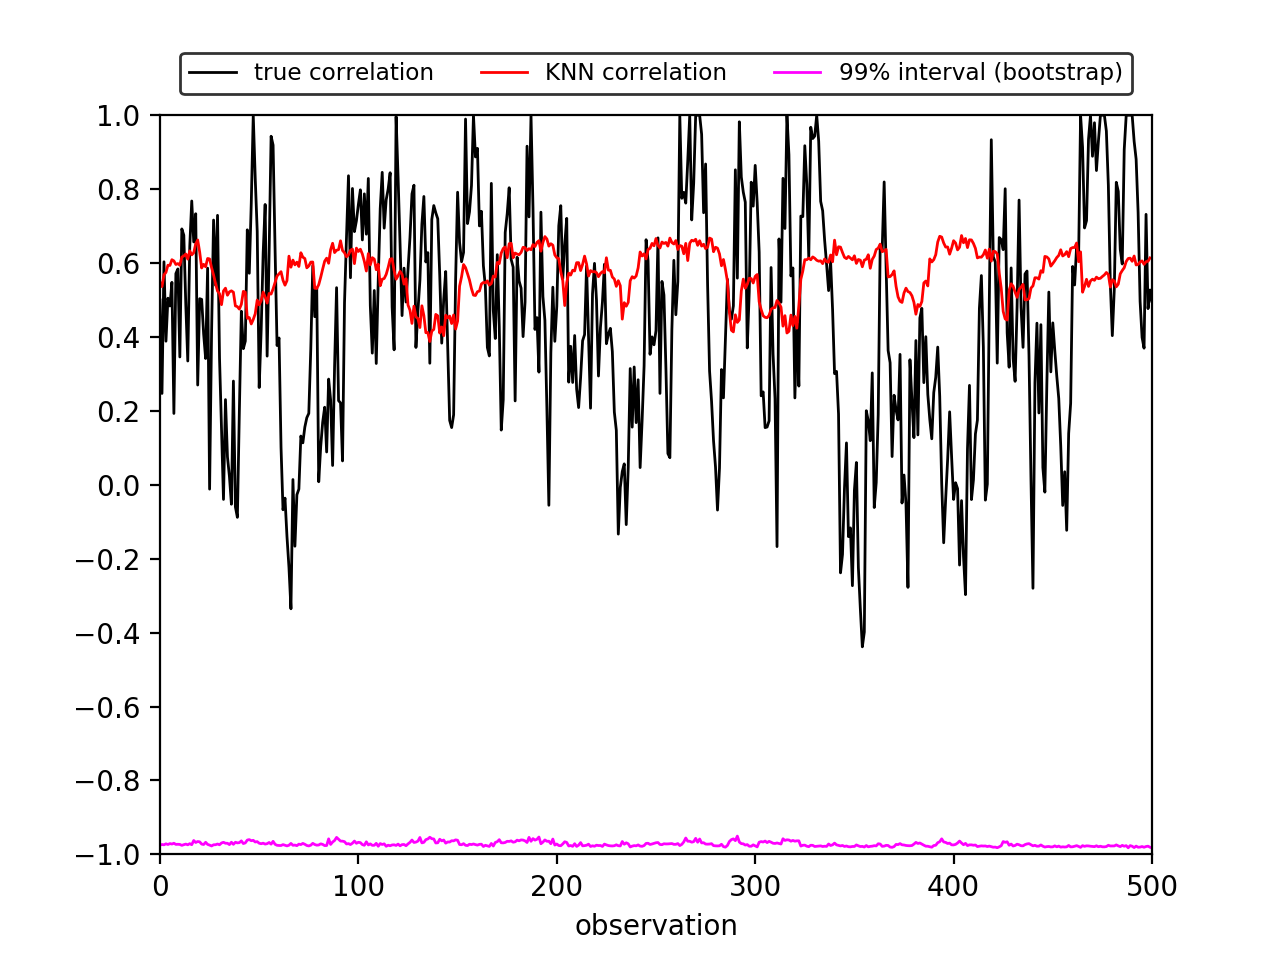
\includegraphics[width=\textwidth]{knn_pearson_21_IDW_estimates_bootstrap_proxy.png} 
		\caption{KNN estimates as inverse distance weighted averages, with window size 21 and Pearson covariates.} 	
		\label{fig:knn_pearson_21_IDW_estimates_bootstrap_proxy}
	\end{subfigure}
	\hfill  
	\begin{subfigure}[b]{0.49 \textwidth}
		\centering 
		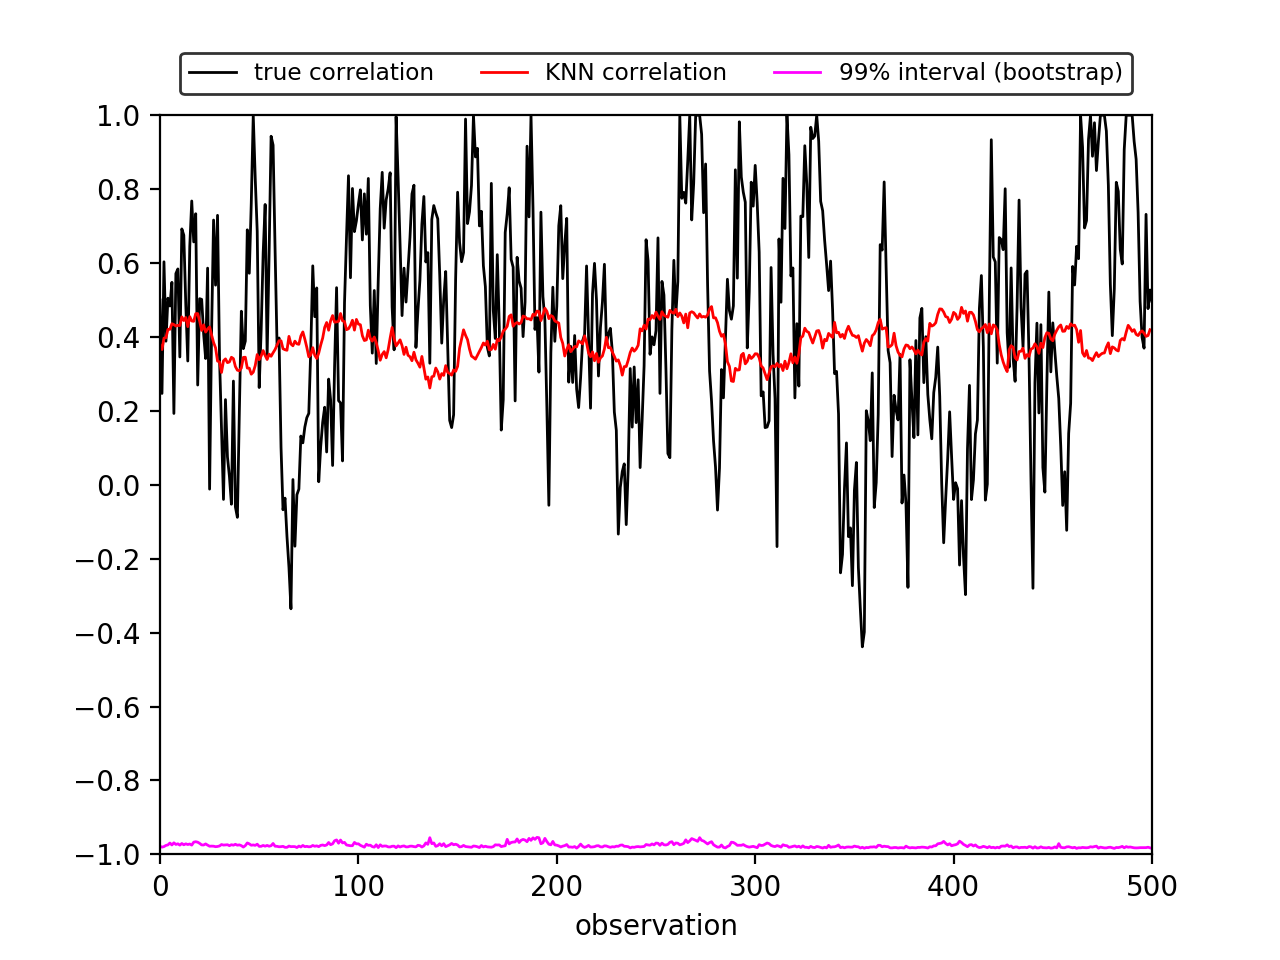
\includegraphics[width=\textwidth]{knn_kendall_21_IDW_estimates_bootstrap_proxy.png} 
		\caption{KNN estimates as inverse distance weighted averages, with window size 21 and Kendall covariates.} 
		\label{fig:knn_kendall_21_IDW_estimates_bootstrap_proxy}
	\end{subfigure}
	\hfill  
	\begin{subfigure}[b]{0.49 \textwidth}
		\centering 
		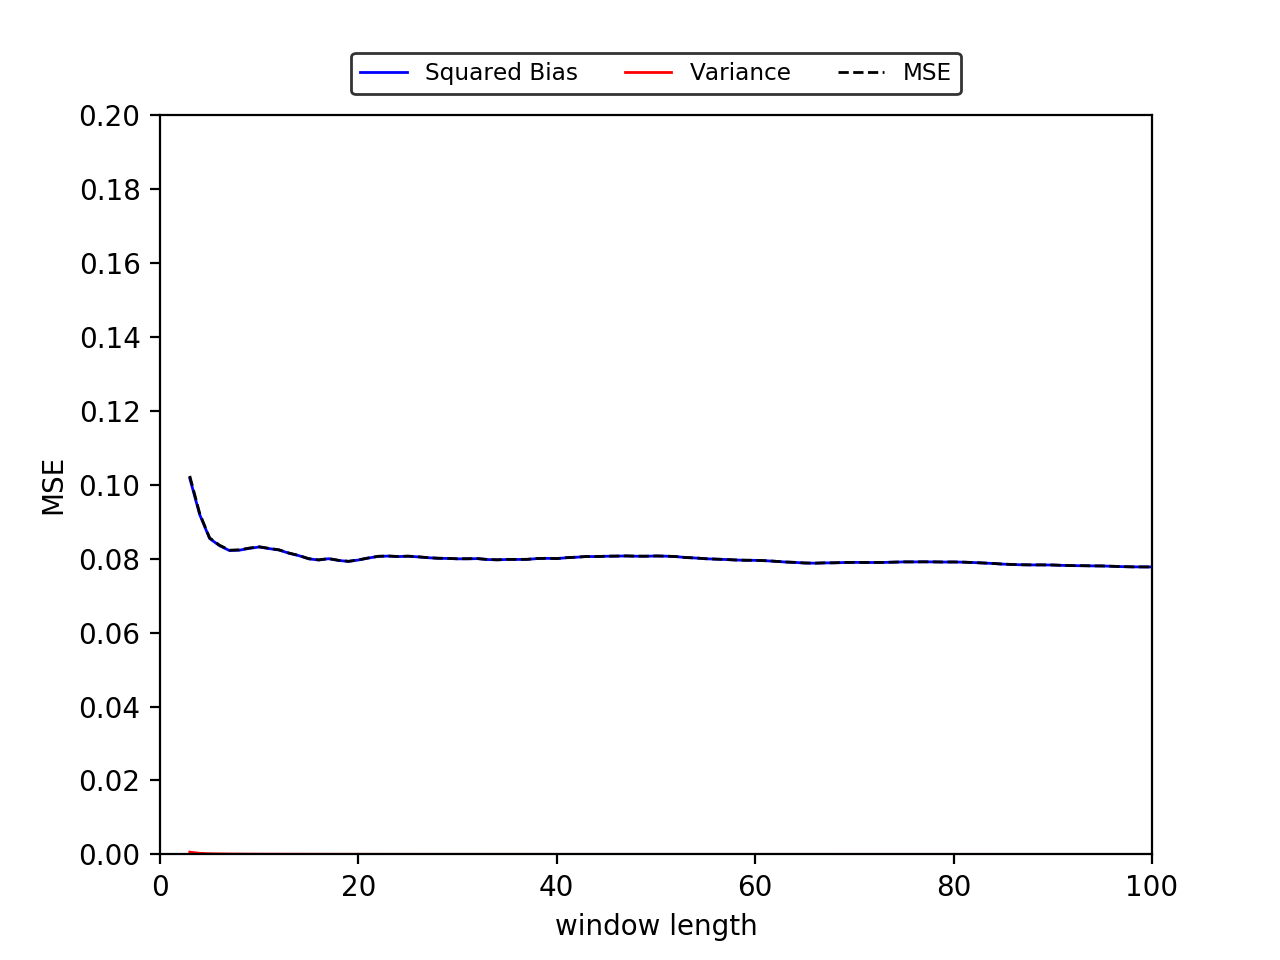
\includegraphics[width=\textwidth]{decom_mse_knn_IDW_pearson_proxy.png} 
		\caption{Bias-variance decomposition for KNN estimates constructed from inverse distance weighted averages and Pearson covariates.} 
		\label{fig:decom_mse_knn_IDW_pearson_proxy}
	\end{subfigure}
	\hfill  
	\begin{subfigure}[b]{0.49 \textwidth}
		\centering 
		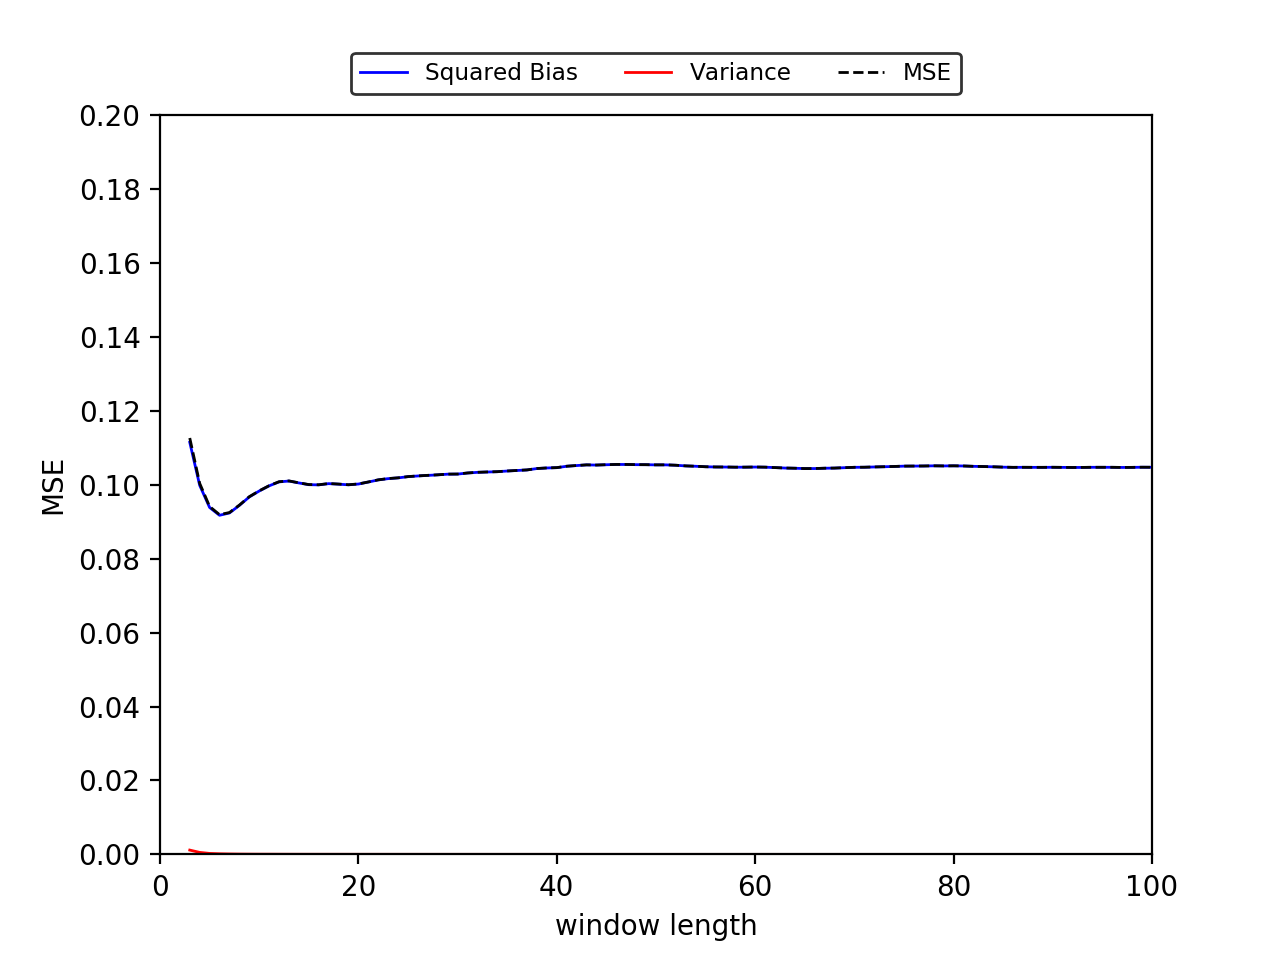
\includegraphics[width=\textwidth]{decom_mse_knn_IDW_kendall_proxy.png} 
		\caption{Bias-variance decomposition for KNN estimates constructed from inverse distance weighted averages and Kendall covariates.} 
		\label{fig:decom_mse_knn_IDW_kendall_proxy}
	\end{subfigure}
	\caption{MSE for KNN estimates with inverse weighting function, Pearson and Kendall Moving Window bootstrap estimates as covariates and response variable.}
	\label{fig:decom_mse_knn_IDW_pearson_kendall_proxy}
\end{figure}


\noindent
Regardless of the choice of window length, MSE from KNN with an uniform weighting function and the set of covariates and response variable constructed from Pearson and Kendall sample correlation estimates using moving windows are approximately between 0.0774 and 0.0923, and 0.1054 and 0.1118, respectively. 
MSE from KNN with an inverse distance weighting function is approximately between 0.0778 and 0.1024, and between 0.0919 and 0.1127, respectively. This implies that, using a KNN estimator, approximations based on Pearson sample correlations using moving windows seems more appropriate for the simulated data than Kendall sample correlations using moving windows, regardless of the weighting function; Fig. \ref{fig:decom_mse_knn_IDW_pearson_proxy} depicts a lower MSE for all window sizes compared with MSE in Fig. \ref{fig:decom_mse_knn_IDW_kendall_proxy}. An explanation for this observation is given along the same lines as for Pearson and Kendall sample correlation estimates using moving windows in Section \ref{sec:true_correlation}; the simulated asset returns follow a multivariate normal distribution, that is, an elliptical distribution. Therefore, it makes sense that lower MSE values are obtained when true correlation is approximated using a linear correlation coefficient such as Pearson in an KNN estimator. Moreover, the choice for an inverse distance weighting function seems to have no significant performance advantage over an uniform weighting function when true correlation is approximated using moving window estimates in terms of a statistical loss functions such as MSE. Interestingly, this is in contrast with results obtained from KNN estimator under true correlation in Section \ref{sec:MSE_knn_true}. More importantly however, using a uniform weighting function with the entire training set yields approximately constant correlation estimates, which is the exact idea we aim to improve on with a more realistic assumption of conditional correlation. The latter is better captured under an inverse distance weighting function. Finally, the variance of MSE from KNN with uniform weighting function and the set of covariates constructed from Pearson and Kendall moving window estimates are approximately 3.98e-6 and 9.26e-7, respectively. The variance of MSE from KNN with inverse distance weighting function and the set of covariates constructed from Pearson and Kendall moving window estimates are approximately 8.46e-6 and 8.61e-6, respectively. The difference in sensitivity to the choice of window length between the different parameterizations is negligible small if significant at all. \\

\noindent
The alternative parameterizations of the KNN estimator also satisfy the positive definiteness condition in the conditional correlation matrix $R_t$ for all time $t$ under all choices of window length in the interval [0, 100]. Fig. \ref{fig:det_knn_len_train_IDW_pearson_kendall_proxy} presents the obtained minimum determinants of $R_t$ for all choices of window length under the proposed alternative parameterizations.\\

\noindent 
This section is concluded with a comparison of the function approximation capabilities of the KNN estimator and Pearson and Kendall sample correlation estimates using moving windows. Comparison is based on MSE between estimated and actual correlations. Fig. \ref{fig:mse_knn5_IDW_pearson_kendall_proxy}\footnote{Only behavior of the (alternative parameterized) KNN estimator with Pearson covariates is shown as behavior of its Kendall counterpart is nearly identical.} shows MSE from KNN under a default parameterization where then number of neighbors equals 5, an alternative parameterization with an inverse distance weighting function as well as Pearson and Kendall sample correlation estimates using moving windows. According to MSE, parameterizations of the KNN estimator with approximated covariates and response variable performs significantly better than those of Pearson and Kendall moving window estimates for small window sizes. Moreover, parameterizations of the KNN estimator with an alternative distance weighting function yields significantly smaller MSE compared to Pearson and Kendall moving window estimates for all window sizes. Thus, similar to the analysis in Section \ref{sec:MSE_knn_alt_true}, the KNN estimator yields lower MSE with an increase in the number of neighbors, particularly for smaller window sizes. This result follows from the fact that conditional correlation is then estimated using increased sample information, which positively contributes to accurately capturing time variation in correlations. Evidently, the underlying correlation dynamics may potentially be best captured optimizing over the hyperparmeter $k$ until an appropriate level of volatility and smoothness is reached. Finally, the variance of MSE from KNN estimates under a default parameterization and alternative parameterization using an inverse distance weighting funtion in Fig. \ref{fig:mse_knn5_IDW_pearson_kendall_proxy} are 5.70e-4 and 8.46e-6, respectively, while that of Pearson and Kendall sample correlation estimates using moving windows are 0.0040 and 0.0037, respectively. In other words, the KNN estimator with approximated covariates and response variable is significantly less sensitive to the choice of window length than Pearson and Kendall sample correlation estimates using moving windows.  \\



\begin{figure}[H] 
	\centering
	\begin{subfigure}[b]{0.49 \textwidth}
		\centering 
		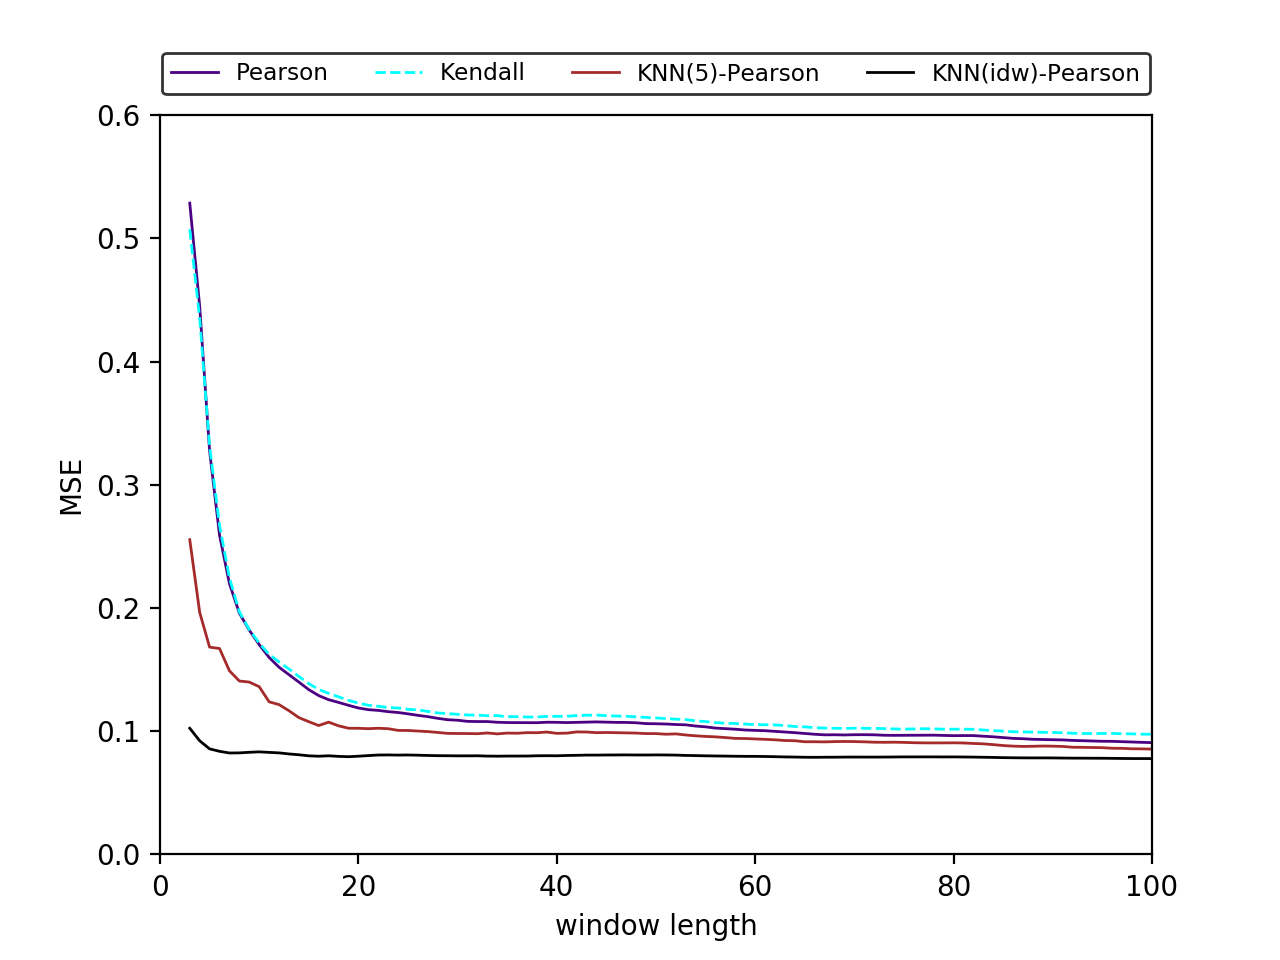
\includegraphics[width=\textwidth]{mse_knn5_IDW_pearson_kendall_proxy} 
		\caption{MSE for KNN with Pearson covariates and proxy correlation, Pearson and Kendall Moving Window bootstrap estimates.}
		\label{fig:mse_knn5_IDW_pearson_kendall_proxy}
	\end{subfigure}
	\hfill
	\begin{subfigure}[b]{0.49 \textwidth} 
		\centering
		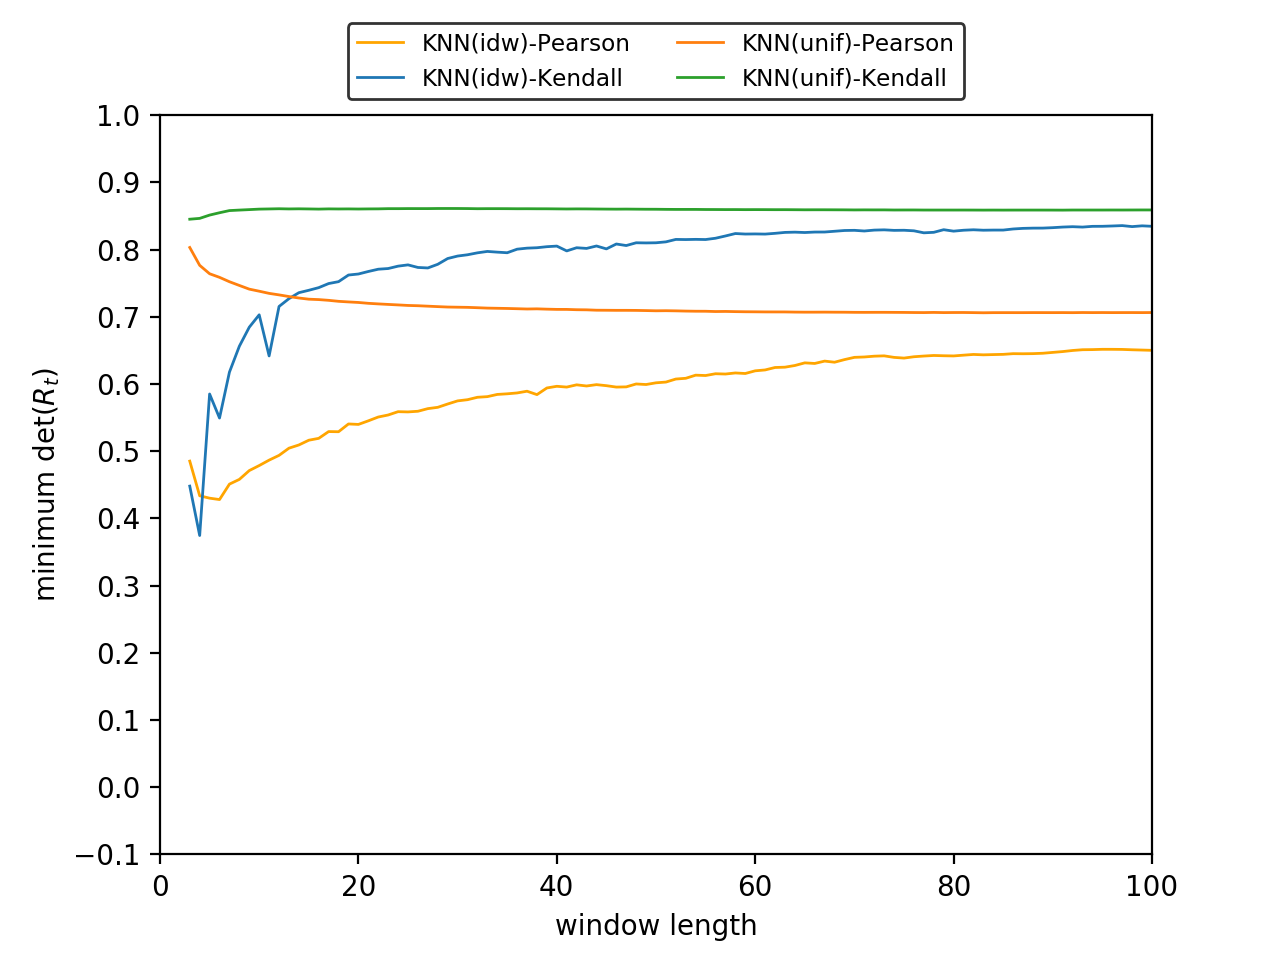
\includegraphics[width=\textwidth]{det_knn_IDW_len_train_pearson_kendall_proxy}
		\caption{Minimum determinants for KNN using uniform and inverse distance weighting function, Pearson and Kendall covariates and proxy correlation.}
		\label{fig:det_knn_len_train_IDW_pearson_kendall_proxy}
	\end{subfigure}	
	\caption{Comparison MSE and minimum determinants for KNN with Pearson covariates and proxy correlation, Pearson and Kendall Moving Window bootstrap estimates.}
	\label{mse_det_knn5_IDW_pearson_kendall_proxy}
\end{figure}



%%%%%%% RANDOM FOREST PROXY %%%%%%%%%%%%%%
\subsection{Generalization Error of Random Forest under Proxy Correlation} \label{sec:MSE_rf_proxy}
The accuracy of RF estimates with Pearson and Kendall covariates for conditional correlation is compared by using the MSE between estimated and actual correlations. MSE from RF with Pearson and Kendall moving window estimates of correlation for covariates and as response variable are shown in Fig. \ref{fig:mse_rf10_pearson_kendall_proxy}. Regardless of the choice of window length, MSE from RF with Pearson and Kendall covariates are between 0.0868 and 0.2318, and 0.0946 and 0.2321, respectively. The variance of MSE from RF estimates with Pearson covariates is approximately 4.54e-4 while that of RF estimates with Kendall covariates is approximately 3.23e-4. Interestingly, Fig. \ref{fig:mse_rf10_pearson_kendall_proxy} shows that MSE from RF estimation with Pearson or Kendall sample approximations for the response variable varies substantially for smaller window sizes. Although, less variation is observed when compared with MSE from Pearson and Kendall sample correlation estimates using moving windows depicted in Fig. \ref{fig:mse_pearson_kendall_bootstrap}. This observation is analogous to the comparison of KNN estimates of correlation. Moreover, RF estimates of conditional correlation where both the set of covariates and response variable is constructed from Pearson and Kendall samples correlation estimates using moving windows satisfy the positive definiteness condition in the conditional correlation matrix $R_t$ for all time $t$ under all considered choices of window length. Fig. \ref{fig:det_rf10_pearson_kendall_proxy} presents the obtained minimum determinants of $R_t$ for all choices of window length. Although the minimum determinants for smaller window sizes approach 0, they remain nonnegative for all time $t$.

\begin{figure}[H]
	\centering
	\begin{subfigure}[b]{0.49 \textwidth} 
		\centering
		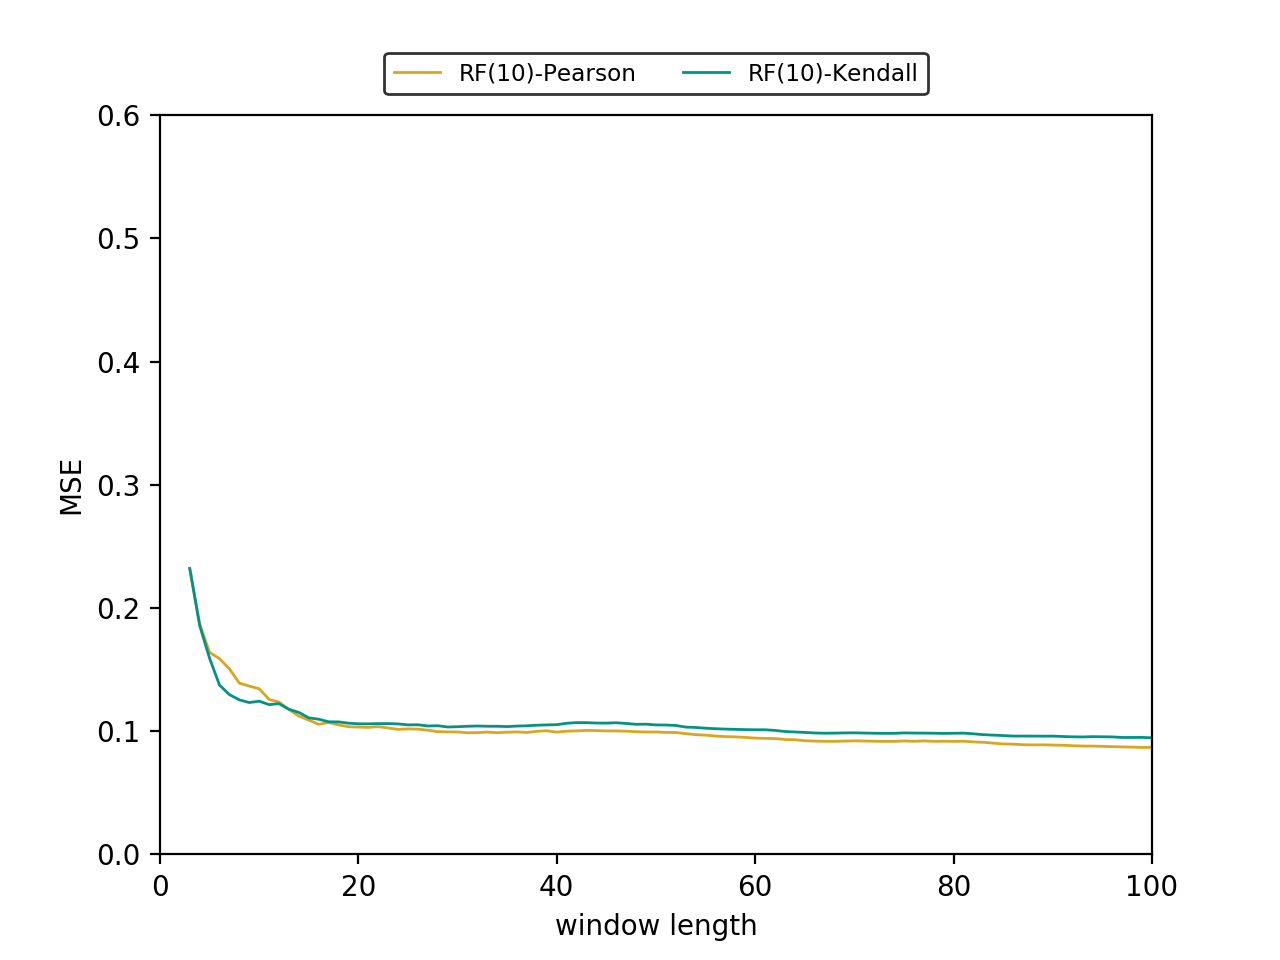
\includegraphics[width=\textwidth]{mse_rf10_pearson_kendall_proxy}
		\caption{MSE for RF with covariates from Pearson and Kendall and proxy correlation.}
		\label{fig:mse_rf10_pearson_kendall_proxy}
	\end{subfigure}
	\hfill
	\begin{subfigure}[b]{0.49 \textwidth} 
		\centering
		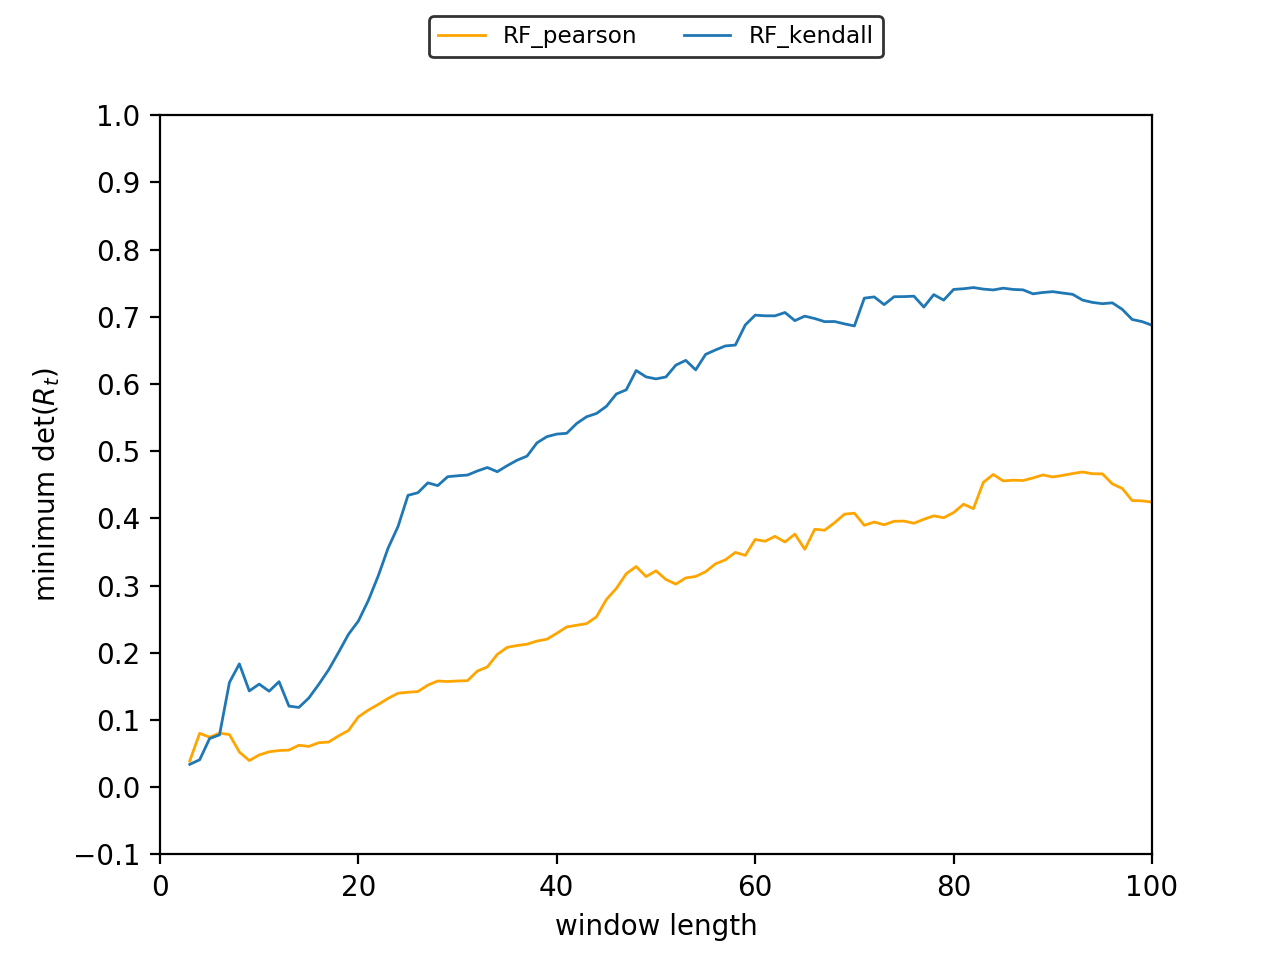
\includegraphics[width=\textwidth]{det_rf10_pearson_kendall_proxy}
		\caption{Minimum determinants for RF with covariates from Pearson and Kendall and proxy correlation.}
		\label{fig:det_rf10_pearson_kendall_proxy}
	\end{subfigure}
	\caption{Comparison MSE and minimum determinants for RF(n\_estimators=10) with covariates from Pearson and Kendall and proxy correlation.}
	\label{fig:mse_det_rf10_pearson_kendall_proxy}
\end{figure}

\noindent
Visual inspection of the plots in Fig. \ref{fig:rf_pearson21_bootstrap_proxy} and Fig. \ref{fig:rf_kendall21_bootstrap_proxy} yields an analysis that is similar to the analysis of the KNN estimator under approximations of correlation instead of actual correlation in Section \ref{sec:MSE_knn_proxy}. It is clear that the uncertainty in the conditional correlation $\rho_t$, which is illustrated by the 99\% confidence interval, is smaller for RF estimates compared to Pearson and Kendall sample correlation estimates using moving windows, even though both the set of covariates and the response variable of the RF estimator are now based on approximations of correlation instead of actual correlation. These figures also show smaller uncertainty in the conditional correlation, $\rho_t$, when compared with RF estimates with true correlation as the response variable, which are depicted in Fig. \ref{fig:decom_mse_rf10_pearson_kendall_true}. Moreover RF estimates of correlation with true correlation as response variable in Fig. \ref{fig:rf_pearson21_bootstrap_true} and Fig. \ref{fig:rf_kendall21_bootstrap_true} are much more volatile. RF estimates with approximated correlation as response variable in Fig. \ref{fig:rf_pearson21_bootstrap_proxy} and Fig. \ref{fig:rf_kendall21_bootstrap_proxy} , however, follow the increases and decreases of the actual correlation smoother, with tighter confidence intervals. This is a more desirable result as it is not expected that correlation between assets changes that drastically at each time unit. \\

\noindent
The MSE decomposition into bias and variance terms from RF estimates of correlation are shown in Fig. \ref{fig:rf_pearson21_bootstrap_proxy} and Fig. \ref{fig:decom_mse_rf10_pearson_proxy}. These figures indicate that the RF estimator with approximated response variable is more sensitive to the choice of the window length for smaller window sizes compared to RF estimator with true correlation depicted in Fig. \ref{fig:decom_mse_rf10_pearson_kendall_true}. This observation is similar to the observation when comparing the KNN estimators with different specifications of the response variable and can be explained by the propagation of approximation error in the response variable. Fig. \ref{fig:decom_mse_rf10_pearson_proxy} and Fig. \ref{fig:decom_mse_rf10_kendall_proxy} show, however, that the RF estimator with approximated response variable is considerably less sensitive to the choice of the window length for smaller window sizes when compared to Pearson and Kendall sample correlation estimates using moving windows depicted in Fig. \ref{fig:decom_mse_pearson} and Fig \ref{fig:decom_mse_kendall}, respectively. Thus, analogous to the KNN estimator with approximated covariates and response variable, the RF estimator seems to mitigate the error propagation to some extend for smaller window sizes. Finally, a lower bias compared to Pearson and Kendall sample correlation estimates using moving windows implies a random forest may be a more suitable estimator for modeling conditional correlation. Additionally, lower variance is observed when compared with Pearson and Kendall sample correlation estimates using moving windows. This can be accredited to the the bootstrap aggregating procedure underlying the RF algorithm as explained in Section \ref{sec:bagging}.        



\begin{figure}[H]  % [h] parameter makes sure figures are located at 'this' location.
	\centering
	\begin{subfigure}[b]{0.49 \textwidth} % sum of widths should be less than text width if all one the same line
		\centering 
		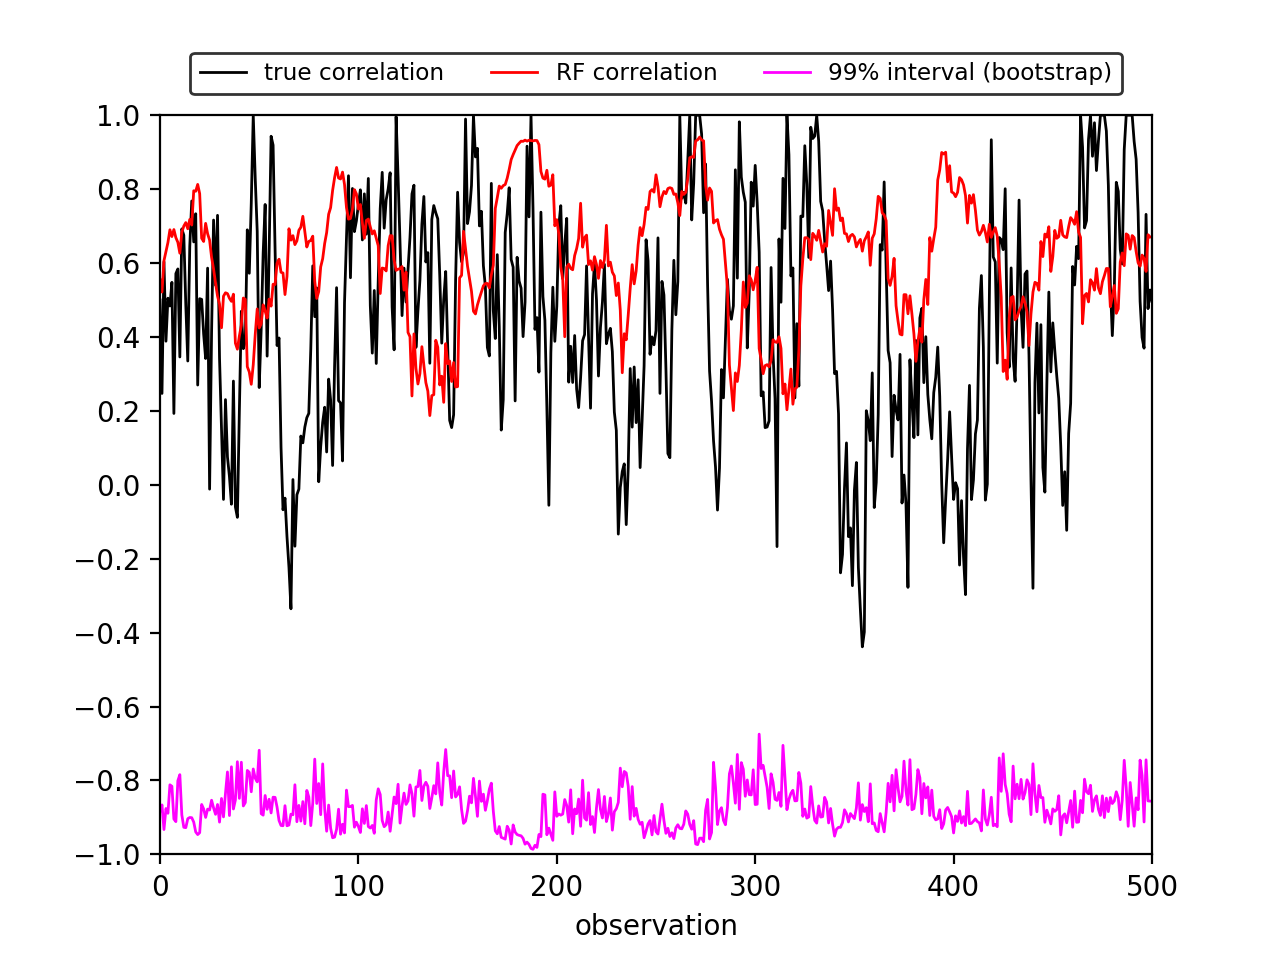
\includegraphics[width=\textwidth]{rf_pearson_21_estimates_bootstrap_proxy.png} 
		\caption{RF estimates with window size 21, Pearson as covariate and proxy correlation.} 	
		\label{fig:rf_pearson21_bootstrap_proxy}
	\end{subfigure} 
	\hfill	
	\begin{subfigure}[b]{0.49 \textwidth} 
		\centering 
		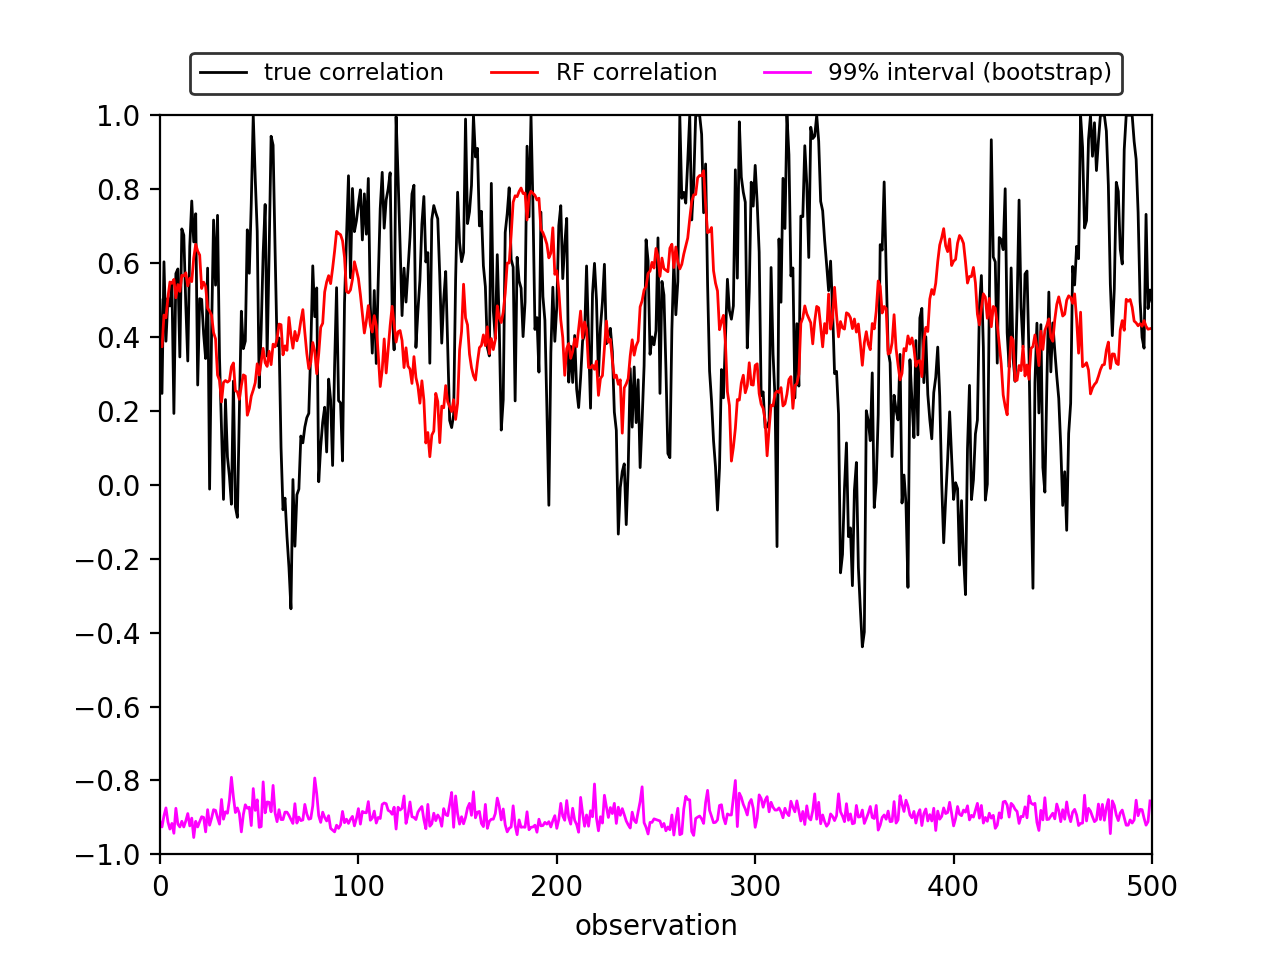
\includegraphics[width=\textwidth]{rf_kendall_21_estimates_bootstrap_proxy.png} 
		\caption{RF estimates with window size 21, Kendall as covariate and proxy correlation.} 
		\label{fig:rf_kendall21_bootstrap_proxy}
	\end{subfigure} 
	\hfill	
	\begin{subfigure}[b]{0.49 \textwidth}
		\centering 		
		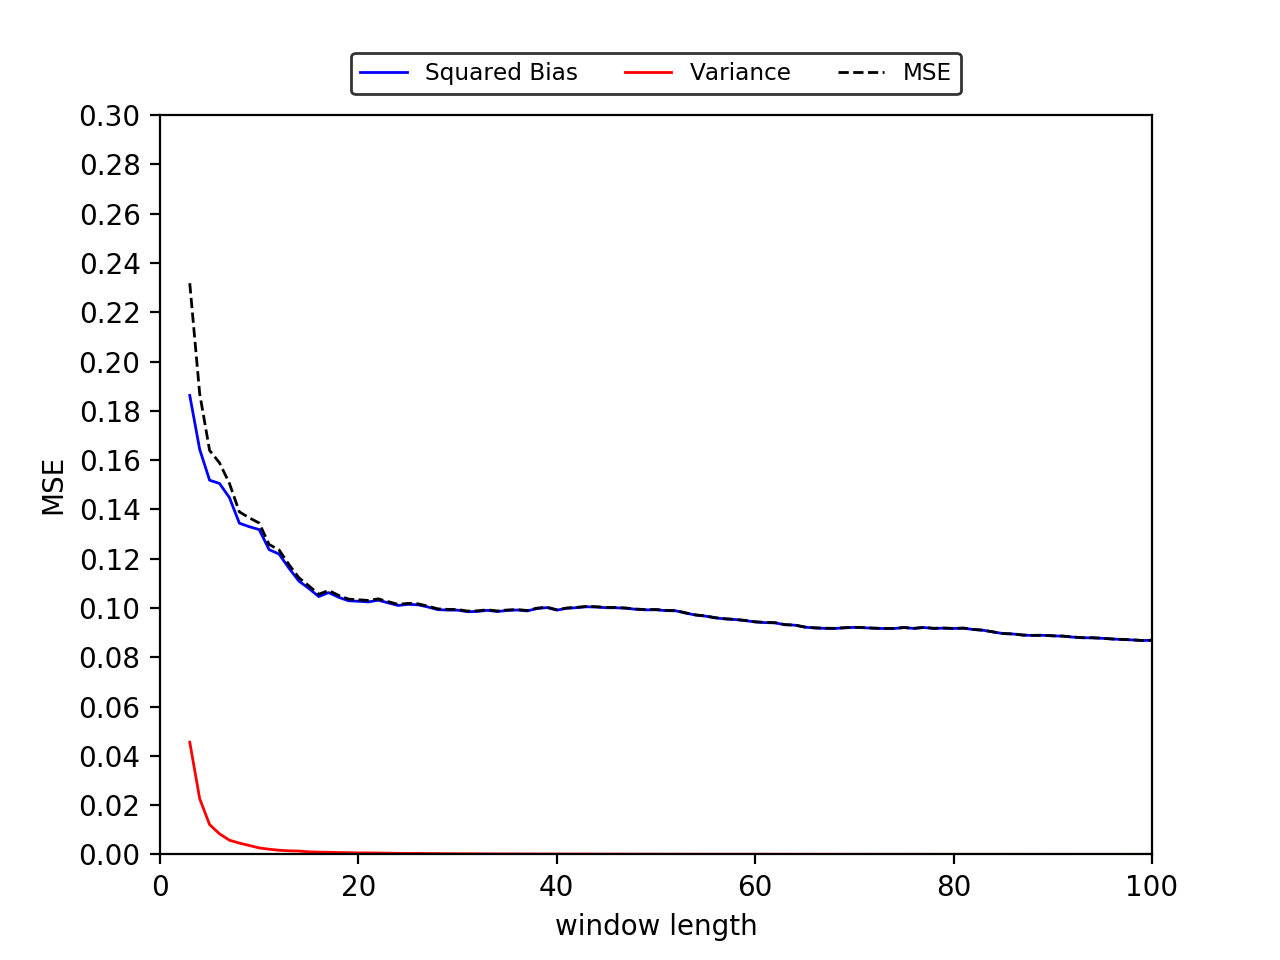
\includegraphics[width=\textwidth]{decom_mse_rf10_pearson_proxy.png} 
		\caption{Bias-variance decomposition for RF estimates with Pearson as covariate and proxy correlation.} 
		\label{fig:decom_mse_rf10_pearson_proxy}
	\end{subfigure}
	\hfill  
	\begin{subfigure}[b]{0.49 \textwidth}
		\centering 
		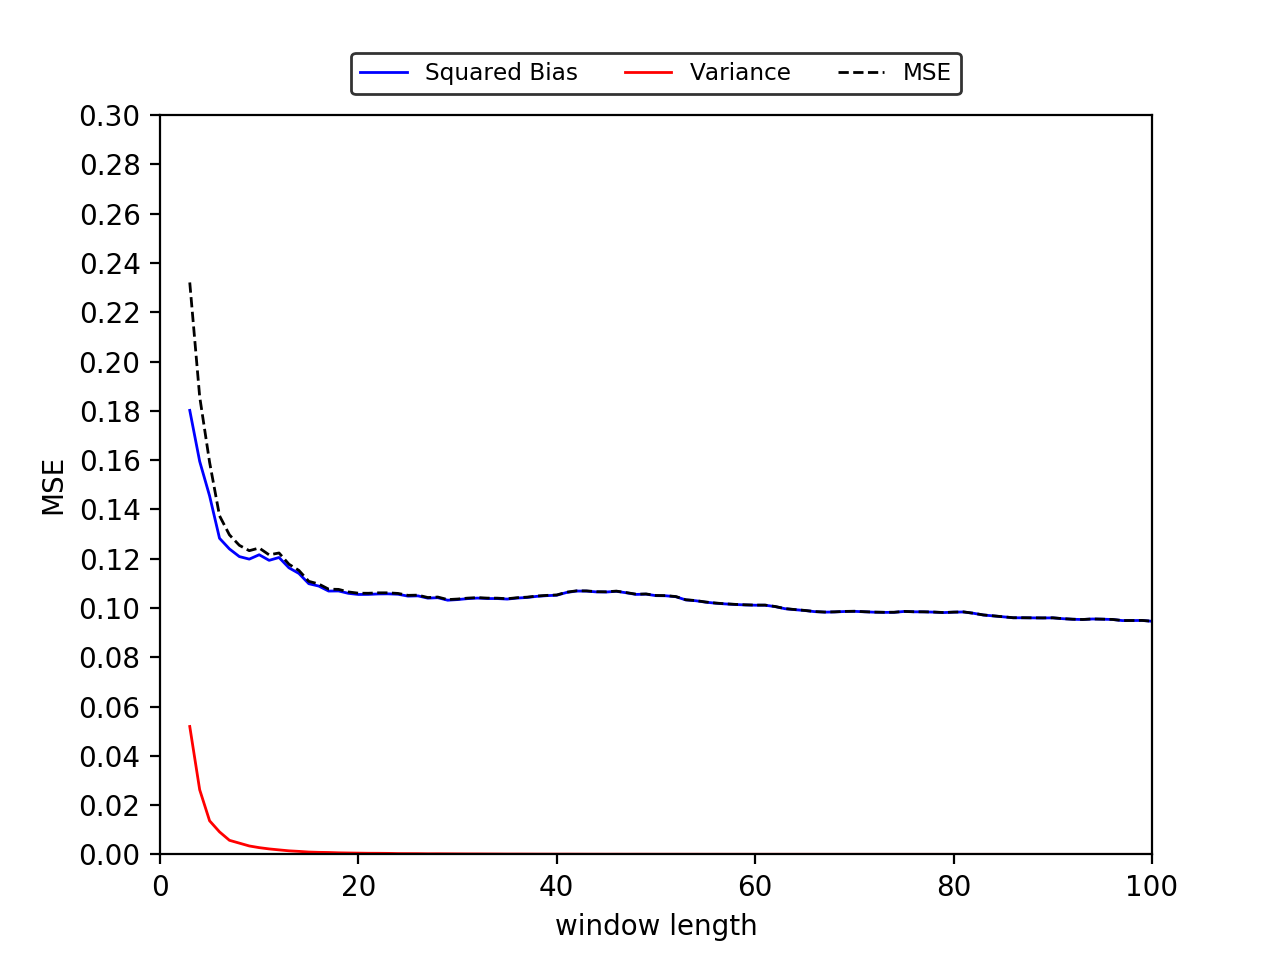
\includegraphics[width=\textwidth]{decom_mse_rf10_kendall_proxy.png} 
		\caption{Bias-variance decomposition for RF estimates with Kendall as covariate and proxy correlation.} 
		\label{fig:decom_mse_rf10_kendall_proxy}
	\end{subfigure}
	\caption{MSE for RF estimates with Pearson and Kendall Moving Window bootstrap estimates as covariates and proxy correlation.}
	\label{fig:decom_mse_rf10_pearson_kendall_proxy}
\end{figure}

\subsection{Effect of Alternative Random Forest Parameterizations under Proxy Correlation} \label{sec:MSE_rf_alt_proxy}
Simulation results in Tabel \ref{tab:mse_decomp_rf_pearson_kendall_proxy}\footnote{Results were obtained by taking 100 bootstrapped samples instead of 1000 due to computational time constraints. This number of bootstrapped samples is however sufficient for illustrational purposes.} show an inverse relationship between the choice of decision trees, or estimators, in the random forest and the uncertainty around the estimated correlations, regardless whether Pearson or Kendall estimates are used for specification of the set of covariates. It is clearly observed that an increase in the number of estimators yields a decrease of the variance, and conversely. This observation is in line with our discussion on MSE decomposition for the RF estimator and Eq. \eqref{eq:variance_rf} from Section \ref{sec:mse_decompose}. For this particular dataset it is observed that the point of diminishing reduction in variance is reached with a smaller amount of trees compared with the sensitivity analysis of the random forest that has true correlation as the response variable. \\

\noindent
With respect to our discussion on the effect of random covariate selection in individual tree construction on the squared bias and variance (for reference, see Section \ref{sec:mse_decompose}: the individual decision trees of the random forest in our simulation are merely decision stumps as the dimension of the covariate set is only three (minimum and maximum returns and pairwise correlation of the previous time unit), $P=3$, which means under default randomization for regression problems $p=P/3 = 1$. As such, no sensitivity analysis is done on the number of covariates given the small dimension of the covariate set. This might, however, may be interesting in case of high dimensional correlation systems. \\  


%% TABLE
\begin{table}[H]
\centering
\captionsetup[subtable]{position=below}
%\captionsetup[table]{position=below}
\begin{subtable}{0.49\linewidth}
\centering
\begin{tabular}{r  c  c  c} 
\toprule
\multicolumn{1}{ r }{\textbf{Trees}} &
\multicolumn{1}{ c }{\textbf{Squared Bias}} &
\multicolumn{1}{ c }{\textbf{Variance}} &
\multicolumn{1}{ c }{\textbf{MSE}} \\
\midrule 

10                                   &   0.1318                       & 0.0026                & 0.1344      \\
100                                 & 0.1320                         & 0.0016               & 0.1335       \\
300                                 & 0.1317                         & 0.0015               & 0.1333       \\
600                                 & 0.1320                         & 0.0015               & 0.1335     \\
1000                               & 0.1319                         &  0.0015              & 0.1334     \\ [1ex]

\bottomrule
\end{tabular}
\caption{MSE for RF estimates with window size 10, Pearson as covariate and correlation.}
\label{tab:mse_decomp_rf_pearson_proxy}
\end{subtable}
\hfill
\begin{subtable}{0.49\linewidth}
\centering
\begin{tabular}{r  c  c  c} 
\toprule
\multicolumn{1}{ r }{\textbf{Trees}} &
\multicolumn{1}{ c }{\textbf{Squared Bias}} &
\multicolumn{1}{ c }{\textbf{Variance}} &
\multicolumn{1}{ c }{\textbf{MSE}} \\
\midrule 

10                                   & 0.1217                         & 0.0027               &  0.1244      \\
100                                 & 0.1219                          & 0.0018               & 0.1236       \\
300                                 & 0.1215                         & 0.0017               &  0.1232      \\
600                                 & 0.1217                         & 0.0017               & 0.1234     \\
1000                               &  0.1214                         &   0.0017             &  0.1230     \\ [1ex]

\bottomrule
\end{tabular}
\caption{MSE for RF estimates with window size 10, Kendall as covariate and correlation.}
\label{tab:mse_decomp_rf_kendall_proxy}
\end{subtable}
\caption{Mean Squared Error (MSE) decomposition as a function of the number of estimators (trees) for RF with approximations for both covariates and response variable.}
\label{tab:mse_decomp_rf_pearson_kendall_proxy}
\end{table}

\noindent
This section is concluded with a comparison of the function approximation capabilities of the RF estimator and Pearson and Kendall sample correlation estimates using moving windows. The comparison is based on MSE between estimated and actual correlations. Fig. \ref{fig:mse_rf10_pearson_kendall_comp_proxy.png} shows MSE from RF under a default parameterization where the number of estimators equals 10, as well as Pearson and Kendall sample correlation estimates using moving windows. According to MSE, default parameterizations of the RF estimator yield significantly smaller MSE compared to Pearson and Kendall sample correlation estimates using moving windows for smaller window sizes. Finally, the variance of MSE from RF estimates under default parameterization and Pearson and Kendall approximations of true correlation in Fig. \ref{fig:mse_rf10_pearson_kendall_comp_proxy.png} are 4.54-4 and 3.23e-4, respectively, while that of Pearson and Kendall moving window estimates are 0.0040 and 0.0037, respectively. \\


\begin{figure}[H]
	\centering
	\begin{subfigure}[b]{0.49 \textwidth} 
		\centering
		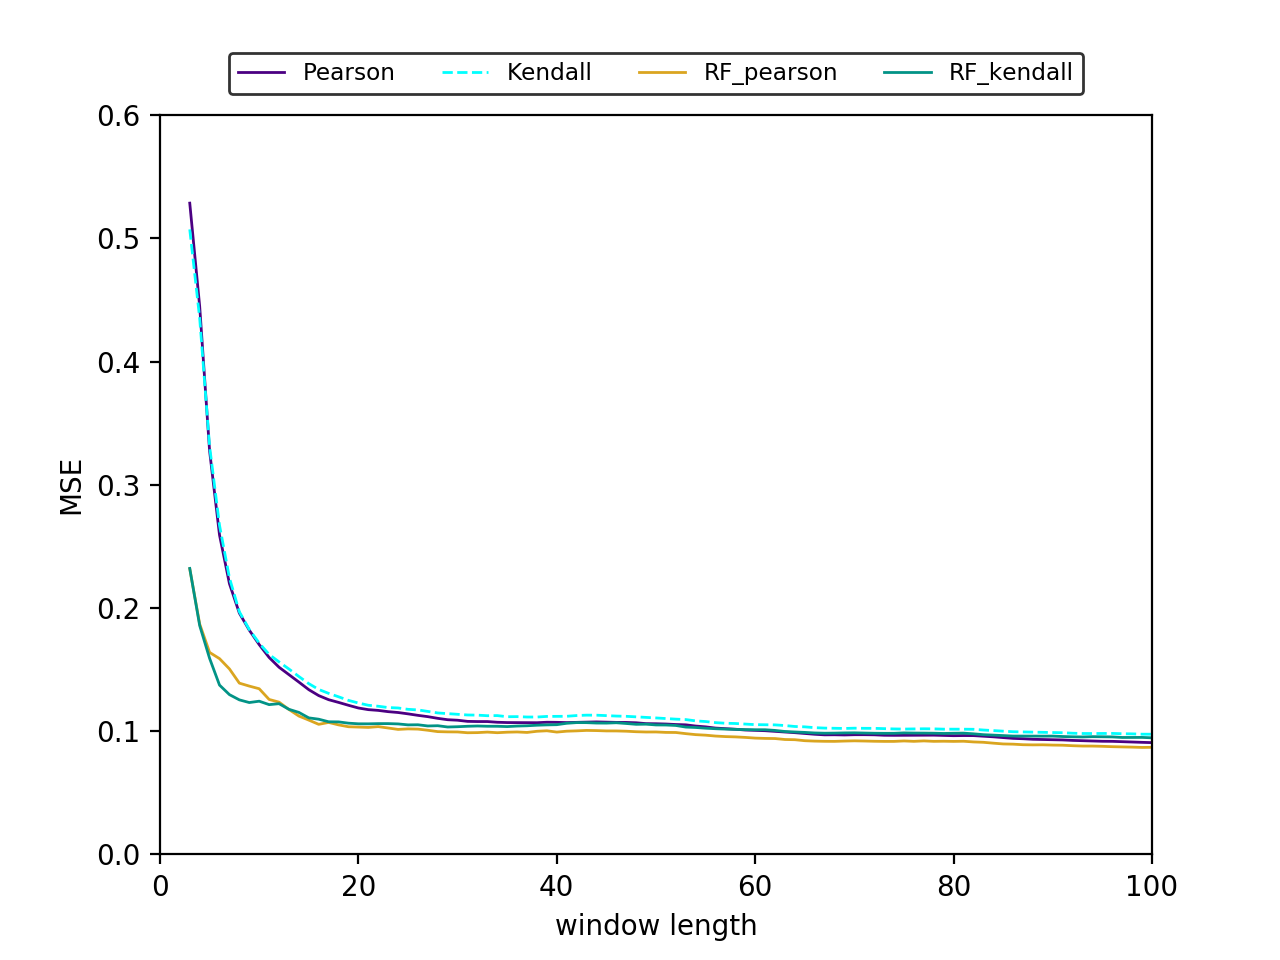
\includegraphics[width=\textwidth]{mse_rf10_pearson_kendall_comp_proxy.png}
		%\caption{MSE for RF with covariates from Pearson and Kendall and proxy correlation.}
		%\label{fig:mse_rf10_pearson_kendall_comp_proxy.png}
	\end{subfigure}
	\caption{Comparison MSE for RF(n\_estimators=10) with proxy correlation, Pearson and Kendall Moving Window bootstrap estimates.}
	\label{fig:mse_rf10_pearson_kendall_comp_proxy.png}
\end{figure}

\iffalse
\noindent
\textbf{Potentially add RF(n\_estimators=100) to show that this parameterization performs even better due to variance reduction. Maybe mentioning this with reference to the sensitivity analysis is also sufficient.} 
\fi









\section{Conclusions Simulation Results} \label{sec:conclusions_sim}
In this chapter, using simulation, performance of parsimoniously specified nonparametric Nearest Neighbor and Random Forest estimators of conditional correlation has been compared against conventional moving windows in terms of a statistical loss function, the mean squared error (MSE). Although conclusions hold for the particular conditional correlation dynamics generated by the data generating process specified in \eqref{eq:correlation_simulation}, the simulation study provides initial evidence on the general use of Nearest Neighbor and Random Forest as nonparametric estimators of conditional correlation between financial variables. The main conclusions may be summarized as follows: \\

\noindent
First, the conditional correlation matrix obtained from the application of Nearest Neighbor and Random Forest estimators satisfies the condition of positive definiteness. A variety of different parameterizations of both learning estimators has been shown to all yield positive definite conditional correlation matrices, regardless whether the response variable was approximated by Pearson or Kendall sample correlation using moving windows or specified by actual correlation.   \\

\noindent
Secondly, both default and alternative parameterizations of proposed learning estimators improve over conventional moving window estimates of conditional correlation in terms of lower MSE, especially for smaller window sizes. Moreover, both default and alternative parameterizations of proposed learning estimators improve over conventional moving window estimates of conditional correlation in terms of decreasing the sensitivity to the choice of window length, which is exhibited through significantly lower variance of MSE. Additionally, the uncertainty in the conditional correlation, $\rho_t$, which is illustrated by 99\% confidence intervals, is smaller for proposed learning estimators compared to Pearson and Kendall sample correlation estimates using moving windows. Additionally, learning estimates with approximated covariates and response variable follow the increases and decreases of the actual correlation smoother, with tighter confidence intervals. This is a more desirable result as it is not expected that correlation between assets changes that drastically at each time unit.     \\

\noindent
Thirdly, both learning estimators, regardless whether the response variable was approximated by Pearson or Kendall sample correlation using moving windows or specified by actual correlation, exhibit expected behavior under different parameterization given the theoretical analysis of the decomposition of MSE into squared bias and variance terms; an increase in the number of neighbors in the Nearest Neighbor algorithm or an increase in the number of decision trees in the Random Forest algorithm reduce the variance in both estimators. Interestingly, an increase in the number of neighbors initially yields a decrease in squared bias where one would have expected an increase in squared bias. As discussed, a potential explanation may be that the inclusion of additional neighbors containing informational value yields more accurate estimates of correlation, that is, a decrease in squared bias. As of a number of additional neighbors, however, only noise is added to the estimation process which results into increased squared bias.      \\


\noindent
In summary, parsimoniously specified Nearest Neighbor and Random Forest estimators improve on predictive capability of conditional correlation compared with Pearson and Kendall sample correlation estimates using moving windows, both in terms of lower MSE and decreasing sensitivity to the choice of window length. Moreover, proposed learning estimators yield positive definite conditional correlation matrices and show expected behavior under different parameterizations in terms of bias variance decomposition of the MSE. As such, using simulation, initial evidence has been provided on the potential application of proposed learning estimators in high dimensional systems of correlations, which is the topic in Chapter \ref{chap:multivariate_analysis}.   


\iffalse
\begin{enumerate}
	\item KNN with true correlation AND KNN with approximated output return positive definite correlation matrices.
	\item RF with true correlation AND RF with approximated output return positive definite correlation matrices.
	\item The difference in accuracy, measured by the MSE, between using Pearson and Kendall approximations of true correlation appear negligible small for the simulation study, regardless whether Nearest Neighbor or Random Forest algorithm was used.  
	\item KNN with true correlation outperforms moving window estimates particularly for smaller window sizes but with full training set and preferably inverse distance weighting function for all window sizes in the interval [3, 100]. A uniform weighting function results in more or less constant correlation, the very idea we try to improve on by considering correlation to be conditional. This result is also obtained when response variable is approximated. Optimization over hyperparameter $k$ shows that with an increase in $k$ variance is reduced (and bias initially) and correlation estimates become increasingly smooth.
	\item RF with true correlation outperforms, even with default parameterization, moving window estimates for all window sizes sizes in the interval [3, 100]. This shows through lower MSE. In addition, RF is far less sensitive to the choice of window length than moving window estimates, which shows through significantly lower variance of MSE. 
	\item Both KNN and RF estimates with true correlation as response variable are rather volatile for under default parameterizations. With an increase in the number of neighbours and trees, the correlation estimates follow follow the increases and decreases of the actual correlation smoother, with tighter confidence intervals.
	\item MSE decomposition behavior KNN with true correlation exactly as expected  given MSE decomposition formulas. Except that with an increase in $k$, we initially observe improved squared bias. Can be explained by the fact that initially an increase in $k$ results in using more data points with informational value for predicting the response variable. After some $k$, the inclusion of more data points results in incorporating noise in the prediction, and we observe an increase in bias.
	\item MSE decomposition behavior RF with true correlation exactly as expected  given MSE decomposition formulas. An increase in number of trees results into diminishing reduction of variance (and, consequently, a decrease in MSE).
	\item Both KNN and RF estimates with approximated correlation as response variable exhibit lower variance than their parameterizations with true correlation as response variable.
	\item RF exhibits higher bias than KNN. RF thus seems less appropriate model at this point. However, given the very small covariate dimension very little decorrelation of trees is possible which would results in variance reduction and possibly MSE reduction (if bias increase is not too big). Given higher dimensional covariate space in context of systems of correlations we continue to opt for RF estimation of conditional correlations. 
	\item Both KNN and RF estimates with approximated correlation as response variable follow the increases and decreases of the actual correlation smoother, with tighter confidence intervals in comparison to KNN and RF estimates with true correlation as the response variable. This is a more desirable result as it is not expected that correlation between assets changes that drastically at each time unit. 
	\item TAKE ALL THE RESULTS FROM ABOVE AND WE HAVE A MAIN RESULT FROM THE SIMULATION STUDY: parsimonious nearest neighbor and random forest models, where the set of covariates and response variable(s) are constructed from approximation of true correlation using Pearson and Kendall moving window estimates, improve on predictive capability of conditional correlation compared with Pearson and Kendall moving window estimates. Moreover, the resulting conditional correlation matrix $R_t$ satisfy the positive definite criterion. This gives enough reason to extend our problem to higher dimensional dataset constructed from real time series data.   
\end{enumerate}
\fi


%%%%%%%%%%%%%%%%%%%%%%%%%%%%%%%%%%%%%%%%%%%%%%%%%%%%%%%%%%%%%%
%%%%%%%%				      SYSTEMS OF CORRELATIONS							%%%%%%%%%
%%%%%%%%%%%%%%%%%%%%%%%%%%%%%%%%%%%%%%%%%%%%%%%%%%%%%%%%%%%%%%
\chapter{Systems of Correlations in Quantitative Financial Risk Management} \label{chap:multivariate_analysis}
This part of the analysis concerns modeling the dependence structure between financial returns in a multivariate setting. Correlation defined by Pearson's linear coefficient and Kendall's $\tau$ coefficient continue to be the measure for dependency. However, the focus of analysis in a multivariate setting is a \textit{system of correlations} rather than \textit{individual correlations}. The role of systems of correlations is demonstrated in the financial task of risk assessment. \\

\noindent
Value-at-Risk is the mandated downside measure for market risk under regulation of the Basel Accords and estimation of conditional volatility is an essential input for calculation of Value-at-Risk in practice. This chapter will illustrate the adequacy of our semiparametric multivariate volatility model in translating the theory of contemporary downside risk assessment into practice for the daily log returns of the 30 constituents included in the Dow Jones Industrial Average index. First, in Section \ref{sec:VaR}, notation is established that is necessary to study the risk of portfolios consisting of an arbitrary number of assets. Section \ref{sec:backesting} then describes the backtesting methodology that is applied to statistically compare our semiparametric multivariate volatility model against a parametric counterpart, the dynamic conditional correlation model of \cite{ref:Engle2002}. Next, our semiparametric multivariate volatility model is applied to the 30 constituents included in the Dow Jones Industrial Average index and performance is verified in terms of an economic loss function, the Value-at-Risk. As such, Section \ref{sec:data} contains some descriptive statistics of the dataset comprising log return series of the 30 constituents included in the Dow Jones Industrial Average index and Section \ref{sec:results} presents the results. Finally, Section \ref{sec:conclusions_emp} concludes the chapter.  \\

\iffalse
\textit{If a multivariate GARCH model is fitted, the multivariate distribution of the returns can be used directly to compute the implied distribution of any portfolio. There is no need to re?estimate the model for different weight vectors. The multivariate approach is illustrated by Giot and Laurent (2003) using a trivariate example with a time?varying correlation model.}

\noindent
\textbf{Once we can estimate conditional CDFs, estimating conditional quantiles follows naturally. That is,
having estimated the conditional CDF we simply invert it at the desired quantile as described in Nonparametric Econometrics: A Primer, Racine (2008), page 28. So: how do we obtain nonparametric conditional CDF estimate for every return given we have conditional covariance estimates and under the assumption that returns follow multivariate Gaussian distribution.}  
\fi



\iffalse
For analysis of the conditional correlations forecasting accuracy implied by different multivariate conditional volatility models, the one day ahead out-of-sample Value-at-Risk ( VaR) is computed and a backtesting analysis is performed. The idea is to consider a  $k$ dimensional system of asset return series, estimate the parameters of multivariate volatility models using a training set and apply the proposed models to obtain out-of-sample one-step-ahead forecasts of the conditional covariance matrix, $H_t$, where the conditional correlation matrix $R_t$ is estimated through learning estimators and the dynamic conditional correlation model of \cite{ref:Engle2002}. Then it is possible to compute one-day-ahead out-of-sample VaR and perform a backtesting analysis.  
\fi



\section{Value-at-Risk Theory} \label{sec:VaR}
One definition of Value-at-Risk ( VaR) is the maximum loss which is not exceeded at a given confidence level $\alpha$, which is analogous to saying VaR is the loss value for which the probability of observing a larger loss is equal to $1-\alpha$. A more formal definition in terms of the $\alpha$-quantile of the loss distribution is given by \citep{ref:QRM2015}, that is,

\begin{align}
	VaR_{\alpha} = inf\{l \in \mathbb{R}:P(L>l) \le 1-\alpha\}=inf\{l \in \mathbb{R}: F_L(l) \ge \alpha\}
\end{align}

\noindent
where $F_L(l) = P(L \le l)$ denotes the distribution function  of the corresponding loss distribution. \\

\noindent
VaR is determined after definition of the portfolio return distribution, where portfolio return $p_t = w' r_t$. It is noted that the validation of the portfolio risk using backtesting measures is not straightforward without further assumptions on $a_t$, the distribution of errors driving the volatility process. In this paper, the multivariate Gaussian distribution is considered for the distribution of $a_t$. In any case, the first two moments of the conditional portfolio return are given by

\begin{align}
	\mathbb{E}[p_t] &= \mu_{p,t} =  w' \mathbb{E}[\mu_t]  \\
	Var[p_t] &= \sigma_{p,t}^2 =  w'H_tw 
\end{align}

\noindent
If the conditional distribution of each asset return is assumed Gaussian, then the portfolio return also follows a Gaussian distribution as the multivariate Gaussian distribution is closed under linear transformations. In that case, the portfolio return distribution is given by

\begin{align}
	p_t \sim \mathcal{N}(w' \mathbb{E}[\mu_t], w'H_tw)  \nonumber
\end{align}

\noindent 
The portfolio VaR under delta-normal assumption for one day horizon at $\alpha$ confidence level is then given by

\begin{align}
	VaR_t(\alpha) &= \mu_{p,t} + \sigma_{p,t} \Phi^{-1}(\alpha)  \label{eq:var_parametric}
\end{align}


\noindent 
where $\Phi$ denotes the cumulative distribution function of standard Gaussian distribution. \\

\iffalse
\noindent
\textbf{Elaborate little bit how VaR is calculated: under assumption of unimodal symmetric distributions computing multivariate quantiles coincides with finding the level hypersurface satisfying the hyperellipsoid equation: $x^T H_t^{-1} x = \chi^2(\alpha)$}. \\
\fi

\noindent
In the backtesting analysis, VaR is computed at different quantiles. For simplicity, but without loss of generality, the unconditional mean is used as the conditional mean filtration given that the dynamic dependence in the conditional means of portfolio returns are generally weak and not significantly affecting VaR results. The VaR for a long position in an equally weighted portfolio is considered as a number of papers \citep{ref:Plyakha2012} suggest that equally weighted portfolio strategies consistently outperform other optimization strategies. Moreover, the focus in this part of the analysis is on the empirical evaluation of different models for modeling and forecasting of the conditional covariance matrix instead of finding optimal portfolio weights or any form of risk minimization.    \\


\iffalse
\subsection{High Density Regions}
\textbf{ALTERNATIVE COMPUTATION OF VAR: Highest Density Regions.}\\
Alternatively, for obtaining VaR (quantiles) from a multivariate normal distribution we can report VaR as the multivariate  'sample quantiles', leading to highest density regions. \\

\noindent
Highest density regions are well suited for the purpose of forecast accuracy evaluation. One of the most distinctive property of HDR's is that of all possible regions of probability coverage $1-\alpha$, the HDR has the smallest region possible in the sample space. In the one-dimensional continuous case that would be the shortest interval, and in the two-dimensional case that would be the smallest area of the surface.   


\begin{itemize}
	\item Highest density region (HDR) ($\alpha$) is defined as the area with the smallest interval that spans $1-\alpha$ of the density.
	\item The region covering the sample space for a given probability $1-\alpha$, should have the smallest possible volume.
	\item Every point inside the region should have probability density at least as large as every point outside the region.
	\item  In the case of a normal distribution an HDR coincides with the usual probability region symmetric about the mean, spanning the a/2 and 1 - a/2 quantiles. 
	\item It follows that the number of disjoint intervals in a highest density region can never exceed the number of modal groups in the density function. 
	\item The inverse cdf of a normal corresponds to the quantile function of a normal.
	\item As long as you can define a function that evaluates the CDF, you can find quantiles. 
	\item  One major problem is the computational  difficulty in numerically integrating over a general region in  high-dimensional space. An alternative approach is required that avoids explicit integration:
\end{itemize}

\noindent
"Although the reduced models, in which the portfolio's returns are considered as one single univariate time series, can be used to calculate VaR for large portfolio, the reduced models (univariate method) may yield low accuracy by ignoring the complicated correlation among the individual returns. Consequently, reduced models provide less detailed information on the source of risk. \iffalse https://pdfs.semanticscholar.org/13c3/84e1928796f06618f812262836c64664db6e.pdf \fi
Problematic: extension of VaR to the multivariate framework is not unique because a unique definition of multivariate quantile does not exist."
\fi


\section{Backtesting Methodology} \label{sec:backesting}
Backtesting is the process of verifying whether one's model performs adequately. In this paper, the goal of a backtesting procedure is to statistically evaluate proposed semiparametric multivariate volatility model against the DCC model of \cite{ref:Engle2002} and potentially detect any misspecification of the risk model. \cite{ref:Christoffersen1998} defined two properties that must both be satisfied by a valid VaR model: unconditional coverage property and independence property. Two statistical tests are considered in this paper for the assessment of these two properties: a failure test of unconditional coverage using the Kupiec test \citep{ref:Kupiec1995} and an independence test using Christoffersen's Markov test \citep{ref:Christoffersen1998}. All test results are provided given a confidence level of 0.95. The test confidence level may be different from the considered quantiles of the loss distribution and the reader is advised not to interchange them. \\

\noindent
\cite{ref:Kupiec1995} developed a statistical test to asses the unconditional coverage of a VaR model; the hypothesis that the the total number of exceedances equals the expected number of exceedances, given the independence property is satisfied. 
\cite{ref:Kupiec1995} tests for unconditional coverage through formulation of a log-likelihood ratio, that is,

\begin{align} \label{eq:Kupiec_test}
	LR_{uc} = 2 \ \text{ln} \Bigg( \bigg(\frac{1-I(\alpha) / T}{1-\alpha}\bigg)^{T-I(\alpha)} \bigg(\frac{I(\alpha) / T}{\alpha} \bigg)^{I(\alpha)}\Bigg)
\end{align}

\noindent
In \eqref{eq:Kupiec_test}, $T$ is the number of observations and $I(\alpha)$ is the total number of exceedances. An exceedance $I_t(\alpha)$ is defined as $r_{t+1} < VaR_t(\alpha)$. The test statistic is asymptotically distributed as a chi-square distribution with 1 degree of freedom under the null hypothesis that the VaR model is adequate, i.e. the VaR model produces an expected proportion of exceedances equal to $\alpha$. Moreover, as the Kupiec test statistic is two sided, the model under consideration is rejected in the following two cases: there are too few exceedances, i.e. the model is excessively conservative, or there are too many exceedances, i.e. an underestimation of risk.   \\

\noindent
An important shortcoming of Kupiec's test is that it solely examines the frequency of exceedances but neglects to assess any form of independence in the occurrence of exceedances. As a consequence, the test may fail to reject a model producing clustered VaR exceedances. This is problematic because, in theory, one would expect exceedances to be evenly spread over time. A clustering of exceedances implies the independence property is violated as an adequate VaR model should exhibit responsiveness to changing market conditions, e.g. changes in volatility and correlations, thereby making clustered exceedances less likely. Exceedance clustering is an important concept as consecutive unexpected losses may be more stressful to an institution compared to unexpected losses occurring somewhat more frequently than expected but are evenly spread out over time  \citep{ref:Campbell2005}. Christoffersen's Markov test \citep{ref:Christoffersen1998} is one of a variety of tests that explicitly examines the independency property of VaR exceedances. The Markov test examines whether the likelihood of a VaR exceedance depends on whether a VaR exceedance occurred on the previous day. Under the null hypothesis, the probability of an exceedance proceeded by a non-exceedance equals the probability of an exceedance proceeded by an exceedance, i.e. $\pi_{01} = \pi_{11}$ in \eqref{eq:Christoffersen_test}. In other words, the probability of exceeding today's VaR should be independent of whether yesterday's VaR was exceeded or not. Only then the VaR measure accurately reflects the underlying portfolio risk \citep{ref:Campbell2005}. \cite{ref:Christoffersen1998} observed that testing for independence can be formulated as a log-likelihood ratio test, that is, 

\begin{align} \label{eq:Christoffersen_test}
	LR_{ind} = -2 \ \text{ln} \Bigg(\frac{(1-\pi_2)^{(n_{00}+n_{10})}\pi_2^{(n_{01}+n_{11})}}{(1-\pi_{01})^{n_{00}}\pi_{01}^{n_{01}}(1-\pi_{11})^{n_{10}}\pi_{11}{^{n_{11}}}} \Bigg)
\end{align}

\noindent
where $n_{ij}$ is the number of transitions from $i$ to $j$ in the hit function series $I_t$, with $i,j \in \{0,1\}$, corresponding to non-exceedances and exceedances. The transition probability $\pi_{ij} = n_{ij} / \sum_j n_{ij} $ and $\hat{\pi}_2 = (n_{01}+n_{11}) / (n_{00}+n_{10}+n_{01}+n_{11})$. Moreover, the test statistic is asymptotically distributed as a chi-square distribution with 1 degree of freedom under assumption of the null hypothesis. \\

\noindent
The main assumption underlying Christoffersen's Markov test is that the indicator function sequence of exceedances and non-exceedances satisfies the Markov property. However, \cite{ref:Christoffersen1998} only considers first order dependence, through a first-order Markov chain model, and this is considered a weakness of the independence test.   \\






\section{Data and Descriptive Statistics} \label{sec:data}
The dataset comprises 30 univariate time series of the log returns included in the 30 Dow Jones Industrial Average index (DJIA). The return series cover data from March 1987 to December 2001 and originate from from Yahoo Finance. During these periods, financial markets experienced tranquil periods with low volatility such as the mid-1990's as well as periods of high volatility, including the collapse of the Dot-com bubble that began in spring 2000 and the collapse of Enron and WorldCom companies in 2001. Fig. \ref{fig:DJIA_returns} shows the daily mean log return series of the DJIA constituents. By visual inspection, the heteroskedastic behavior of the return series becomes apparent, indicating volatility clustering, and is an indication for specifying a model for the conditional variances to capture this behavior.        


\begin{figure}[H]
	\centering
	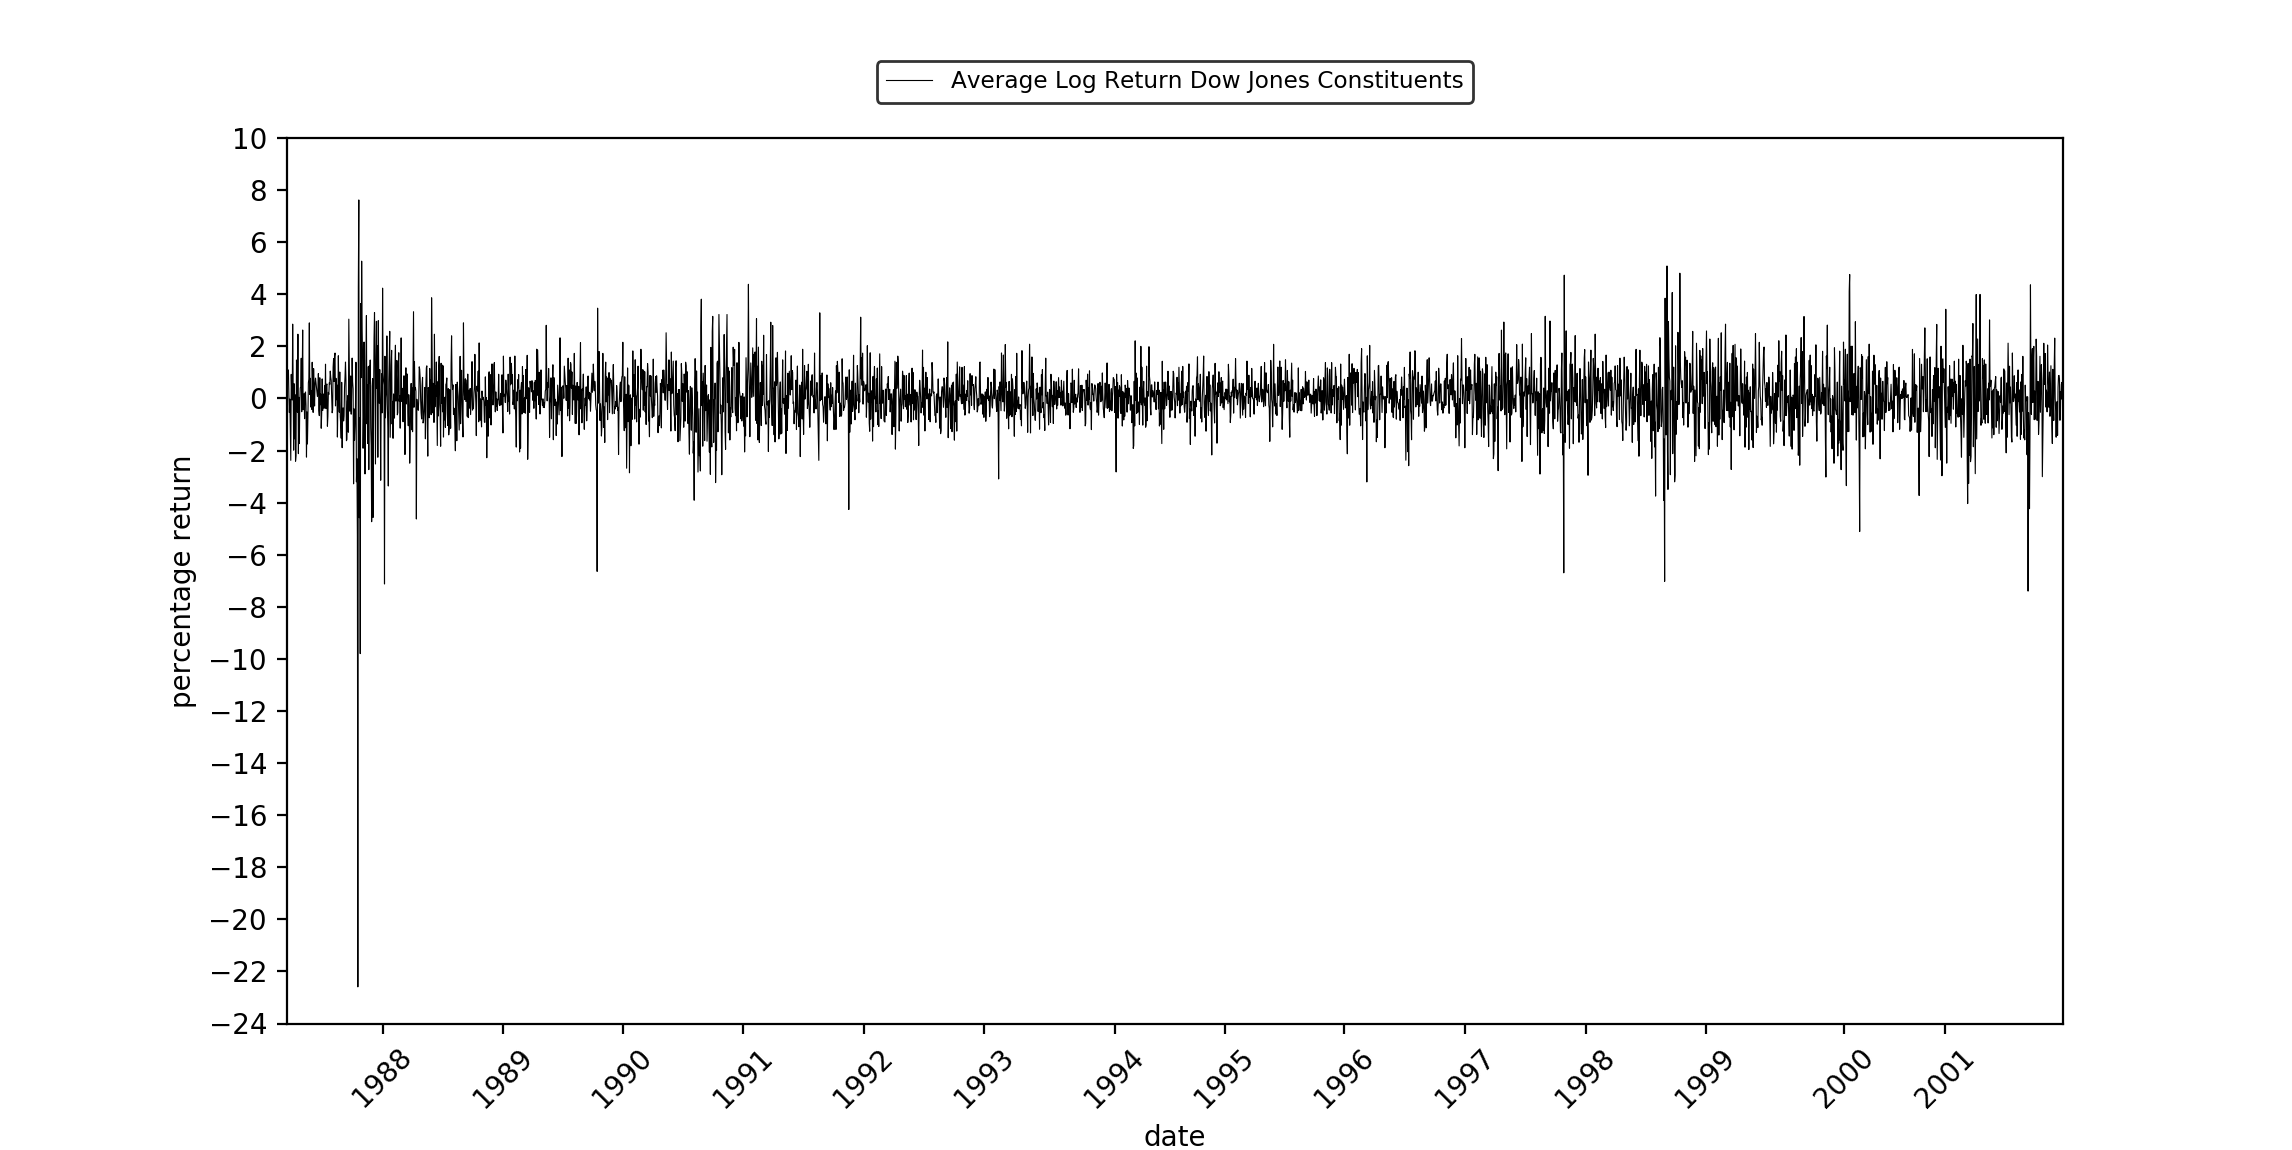
\includegraphics[scale=0.6]{multivar_analysis/log_returns_DJ_constituents.png}
	\caption{Log return of equally weighted Dow Jones constituents from March 1987 to December 2001.}
	\label{fig:DJIA_returns}
\end{figure}

\subsection{Summary Statistics}
Tabel \ref{tab:stats_data} presents summary statistics on the 30 marginal time series of the log returns included in the DJIA. Of particular note is the negative skewness of the return series and the excess kurtosis for all 30 assets. \iffalse www.tandfonline.com/doi/pdf/10.1080/07350015.2016.1177535?needAccess=true \fi All asset return series exhibit an excess kurtosis indicating a higher probability of large negative and positive returns than would be expected under normality. Additionally, all return series exhibit negative skewness which indicates more frequent large negative returns than large positive returns. In other words, all series exhibit behavior that departs from normality. The departures from normality are verified with a simple Jarque-Bera test \citep{ref:Jarque1980} under the null hypothesis that the sample is drawn from a distribution with a skewness and excess kurtosis equals to that of the normal distribution, that is, skewness and excess kurtosis are zero. The Jarque-Bera test rejects the assumption of normality for all assets. This motivates considering specifications for the conditional variance and marginal error distributions in order to capture the exhibited excess kurtosis and skewness. 


\begin{table}[H]
\centering
\captionsetup[subtable]{position=below}
\begin{tabular}{l c c c c c c c}
\toprule
\multicolumn{1}{ c }{\textbf{Asset}} &
\multicolumn{1}{ r }{\textbf{Mean}} &
\multicolumn{1}{ r }{\textbf{St. dev}} &
\multicolumn{1}{ r }{\textbf{Skewness}} &
\multicolumn{1}{ r }{\textbf{Ex. kurtosis}} &
\multicolumn{1}{ r }{\textbf{Minimum}} &
\multicolumn{1}{ r }{\textbf{Maximum}} &
\multicolumn{1}{ c }{\textbf{Jarque-Bera}}  \\
\midrule 
AA    & 0.0601 & 2.071   & -0.4802  & 11.36        & -27.46  & 13.13   & 20172  \\
AXP   & 0.0407 & 2.272   & -0.7064  & 11.99        & -30.34  & 17.12   & 22613  \\
BA    & 0.0402 & 1.964   & -0.5576  & 9.10         & -19.39  & 14.22   & 13054  \\
BAC   & 0.0562 & 2.070   & -0.2483  & 5.21         & -20.76  & 10.88   & 4253   \\
C     & 0.0747 & 2.328   & -0.6653  & 10.27        & -26.43  & 16.85   & 16638  \\
CAT   & 0.0481 & 2.054   & -0.5227  & 9.08         & -24.42  & 13.59   & 12963  \\
CVX   & 0.0478 & 1.549   & -0.4946  & 8.06         & -18.13  & 9.04    & 10232  \\
DD    & 0.0359 & 1.812   & -0.3979  & 6.45         & -20.19  & 8.37    & 6551   \\
DIS   & 0.0413 & 2.074   & -1.3173  & 27.44        & -34.26  & 17.56   & 117944 \\
GE    & 0.0689 & 1.713   & -0.4117  & 8.00         & -19.47  & 11.75   & 10041  \\
GM    & 0.0282 & 1.984   & -0.4274  & 7.61         & -23.63  & 13.71   & 9091   \\
HD    & 0.1224 & 2.334   & -1.2136  & 18.04        & -33.86  & 12.14   & 51412  \\
HPQ   & 0.0389 & 2.638   & -0.2964  & 6.21         & -22.64  & 15.91   & 6031   \\
IBM   & 0.0417 & 2.009   & -0.6378  & 14.46        & -26.82  & 12.36   & 32714  \\
INTC  & 0.1009 & 2.897   & -0.4263  & 6.08         & -24.89  & 22.65   & 5846   \\
JNJ   & 0.0704 & 1.660   & -0.4638  & 8.20         & -20.44  & 10.57   & 10564  \\
JPM   & 0.0422 & 2.314   & -0.6260  & 13.22        & -32.35  & 14.77   & 27356  \\
AIG   & 0.0694 & 1.701   & -0.2275  & 5.21         & -17.19  & 10.48   & 4247   \\
KO    & 0.0624 & 1.797   & -0.7580  & 21.66        & -28.29  & 17.91   & 73197  \\
MCD   & 0.0417 & 1.745   & -0.3339  & 6.20         & -18.28  & 10.31   & 6039   \\
MMM   & 0.0488 & 1.586   & -0.8289  & 14.45        & -22.58  & 10.50   & 32827  \\
MRK   & 0.0600 & 1.735   & -0.1886  & 3.56         & -13.93  & 9.27    & 1988   \\
MSFT  & 0.1271 & 2.602   & -0.9667  & 16.21        & -37.95  & 17.85   & 41368  \\
PFE   & 0.0772 & 1.942   & -0.3331  & 4.48         & -18.92  & 9.89    & 3182   \\
PG    & 0.0608 & 1.837   & -3.1385  & 68.07        & -35.99  & 19.80   & 725300 \\
T     & 0.0523 & 1.705   & -0.1757  & 3.85         & -13.52  & 10.67   & 2314   \\
UTX   & 0.0530 & 1.827   & -1.5147  & 24.37        & -30.29  & 9.87    & 93592  \\
VZ    & 0.0435 & 1.679   & -0.1381  & 8.58         & -19.31  & 13.18   & 11430  \\
WMT   & 0.0769 & 2.054   & -0.0796  & 2.69         & -12.50  & 11.47   & 1128   \\
XOM   & 0.0511 & 1.528   & -1.0537  & 30.83        & -26.77  & 16.54   & 148221\\ [1ex]
\bottomrule  
\end{tabular}
\caption[Descriptive statistics of Dow Jones Industrial Average daily log returns.]{Descriptive statistics of Dow Jones Industrial Average daily log returns. Tick symbol is used to denote the company and critical value of the Jarque-Bera test statistic is 5.99. Log returns are in percentages and the sample period is from March 1987 to December 2001 for 3735 observations.} 
\label{tab:stats_data}
\end{table}

\subsection{Conditional Variance Model}
As discussed in Section \ref{sec:VaR}, for simplicity, but without loss of generality, the conditional mean of our data is specified by the unconditional mean. Our model for the conditional variance is the GARCH(1,1) model of \cite{ref:Bollerslev1986} with the marginal distributions of the standardized residuals specified as the Gaussian distribution. Additionally, we consider the asymmetric volatility model of \cite{ref:Glosten1993}, the GJR-GARCH model, as specification for the conditional variance. The choice for the asymmetry in this model is motivated by the asymmetric response of volatility to positive and negative asset returns; a asymmetric negative correlation between asset return change and volatility change implies that the rise in volatility following negative returns is generally larger than the fall in volatility following positive returns. The GJR-GARCH(1,1) model accounts for this inverse relationship between first and second order moments of asset returns, that is,

\begin{align} \label{eq:gjr_garch}
	\sigma^2_{i,t} = \omega_i + \beta_i \sigma^2_{i,t-1} + \alpha_i a^2_{i,t-1} + \gamma_i a^2_{i,t-1} I_{t-1}\{a_{i,t-1} < 0 \} 
\end{align}

\noindent
For the marginal distributions of the standardized residuals from GJR-GARCH specification for the conditional variance, the following specification is considered: skewed Student's t-distribution of \cite{ref:Hansen1994}, which accounts for nonzero skewness and excess kurtosis, that is, 

\begin{align}
	\eta_{i,t} = \frac{z_{i,t}}{\sigma_{i,t}} \sim \text{iid} \ Skew \ t (v_i, \psi_i)  \nonumber
\end{align}


\noindent
Table \ref{tab:stat_dist_gjr_sstd_table} summarizes the results of estimating the GJR-GARCH(1,1) model from \eqref{eq:gjr_garch} on the daily log returns of 30 constituents included in the DJAI for the initial in-sample period of the volatile market test period (March 1987 to December 1999) for 3235 observations. A Ljung-Box test \citep{ref:Ljung1978} exhibits significant autocorrelation in 15 out of 30 of the daily log returns. For the purpose of verifying the adequacy of the conditional variance and marginal distribution specifications, an ARMA(3,1) model was used to capture autocorrelation remaining in the residual series. The conditional variance models display only moderate statistical indication of asymmetry in volatility given that the estimated asymmetry coefficient, $\gamma_i$, is found statistically significant for only 8 out of 30 assets. However, the sign bias test statistics on the residuals are insignificant for 7 out of 8 of the asymmetric models implying asymmetric response of volatility to positive and negative asset returns is adequately captured by the asymmetric GJR-GARCH model. Moreover, for 6 out of these 7 the effect of positive asset returns are stronger than negative asset returns on future volatility. The average estimated degrees of freedom of the shape parameter is 6.9 and the estimated skewness parameter is positive for all 30 assets, and both estimated parameters are significantly different from zero for all 30 assets, indicating heavy tails and positive skewness.    

\begin{table}[H]
\centering
\captionsetup[subtable]{position=below}
\begin{tabular}{l c c c c c c c}
\toprule
\multirow{2}{*}{}      & \multicolumn{7}{c}{Cross-sectional distribution}                                        \\ \cmidrule{3-8} 
                    &   & Mean       & 5\%       & 25\%      & Median    & 75\%               & 95\%              \\ \midrule 
$\omega_i$         &        & 0.0965     & 0.0211    & 0.0384    & 0.0713    & 0.1023             & 0.2856            \\
$\alpha_i$           &       & 0.0355     & 0.0123    & 0.0281    & 0.0359    & 0.0404             & 0.0600            \\
$\beta_i$             &     & 0.9208     & 0.8840    & 0.9036    & 0.9279    & 0.9416             & 0.9650            \\
$\gamma_i$        &          & 0.0357     & 0.0009    & 0.0135    & 0.0377    & 0.0580             & 0.0734            \\
$v_i$                  &   & 6.9225     & 4.7454    & 6.2507    & 7.0366    & 7.7493             & 8.4095            \\
$\psi_i$               &     & 1.0406     & 1.0043    & 1.0247    & 1.0390    & 1.0529             & 1.0830            \\
\multicolumn{6}{l}{}                                                    & \multicolumn{2}{l}{No. of  Rejections} \\
\multicolumn{6}{l}{LB test for standardized residuals}                  & \multicolumn{2}{c}{2}                  \\
\multicolumn{6}{l}{WP test for squared standardized residuals} & \multicolumn{2}{c}{2}                  \\
\multicolumn{6}{l}{KS test for skew t dist standardized residuals}      & \multicolumn{2}{c}{1}     \\ [1ex]            
\bottomrule  
\end{tabular}
\caption[Summary statistics of GJR-GARCH skewed Student's t model specification for the conditional variance in volatile market conditions.]{Summary statistics of GJR-GARCH(1,1) skewed Student's t model specification for the conditional variance in the initial in-sample period of the volatile market period.} 
\label{tab:stat_dist_gjr_sstd_table}
\end{table}

\noindent
We conclude our discussion on the GJR-GARCH(1,1) model with skewed Student's t-distributed marginals summarizing goodness-of-fit tests for the marginal distribution specification. Table \ref{tab:stat_dist_gjr_sstd_table} shows that a Ljung-Box test for autocorrelation up to the tenth lag rejects the null hypothesis of zero autocorrelation (at the 0.05 level) for only two of the standardized residual series. More importantly, the weighted portmanteau test \citep{ref:Fisher2012} rejects the null hypothesis of zero autocorrelation (at the 0.05 level) up to the tenth lag for only two of the squared standardized residual series. From the latter one can conclude that the GJR-GARCH(1,1) model provides a satisfactory fit to the conditional volatilities. Next, the null hypothesis  of correct specification of the skewed Student's t-distribution for the standardized residuals is rejected for 1 of the 30 asset return series with a Kolmogorov-Smirnov test using 100 simulations. Table \ref{tab:stat_dist_garch_norm_table} summarizes the results of the estimated ARMA(3,1)-GARCH(1,1) model with Gaussian marginal distribution. The table provides strong statistical evidence on misspecification of the Gaussian distribution for the marginal distributions of the standardized residuals as the null hypothesis of correct specification of the Gaussian distribution for the standardized residuals is rejected for all asset return series with a Kolmogorov-Smirnov test using 100 simulations. \\

\noindent
In summary, we can conclude that the GJR-GARCH(1,1) model with a skewed Student's t-distribution specification for the marginal errors provides an adequate alternative  conditional variance model that is capable of capturing the excess kurtosis and skewness exhibited by the daily log returns of the 30 DJIA constituents in our empirical application. This holds for the initial in-sample period of the volatile market test period (March 1987 to December 1999) but similar conclusions hold for the initial in-sample period of the tranquil market test period (March 1987 to December 1993) as supported by Tabel \ref{tab:stat_dist_gjr_sstd_tranquil_table} and Tabel \ref{tab:stat_dist_garch_norm_tranquil_table}.  


\section{Empirical Results} \label{sec:results}
Model adequacy is verified under tranquil market conditions (mid-1990's) and volatile market conditions (the Dot-com bubble) by considering the following backtest periods; (1) an out-of-sample period from January 1994 to December 1995 for 504 observations corresponding to tranquil market conditions with an initial in-sample period from March 1987 tot December 1993 for 1720 observations; (2) an out-of-sample period from January 2000 to December 2001 for 500 observations corresponding to volatile market conditions with an initial in-sample period from March 1987 tot December 1999 for 3235 observations. \\

\noindent  
Our empirical application proceeds as follows. Using daily log returns of the 30 constituents included in the Dow Jones Industrial Average index for the in-sample estimation period, we 


\begin{enumerate}
	\item Estimate conditional volatility models for each asset
	\item Use estimates of conditional volatility models to form one-step-ahead conditional volatility forecasts for each asset 
	\item  Estimate nonparametric conditional correlation models
	\item Use estimates of conditional correlation model to form one-step-ahead pairwise correlation forecasts
	\item Combine conditional correlation forecasts with conditional volatility forecasts to construct the conditional covariance matrix forecast
	\item Use the conditional covariance matrix forecast to obtain Value-at-Risk forecasts
	\item Backtest Value-at-Risk forecasts
\end{enumerate} 

\noindent
One-step-ahead out-of-sample forecasts are obtained for the entire out-of-sample period. Conditional volatility and conditional correlation model parameters are re-estimated with the most recent information available, that is, conditional on the information available at time $t-1$. The result is a set of Value-at-Risk forecasts that corresponds in size to the length of out-of-sample period. \\



\bigskip
\noindent
"The confidence level is of importance. Evidently, the higher the confidence level, the larger the Value-at-Risk of the portfolio. By varying the confidence level, one is able to explore a whole risk profile, i.e. the entire distribution of results is revealed." \\


\noindent
\textbf{When commenting on the test results, do this from a perspective of rejecting the corresponding null hypothesis and whether the models underestimate risk or are overly conservative. And the practical implications from a regulatory perspective and a hedge fun/ bank perspective: a high-level capital reserve or low-level capital reserve. When commenting on figures with VaR functions talk about underestimation/ overestimation of sudden change in volatilities. Comment structure: First comment on test statistics depicted in tables (Coverage and Independence), then comment on figures containing, returns and VaR estimates of different models under the same VaR level.} \\

\iffalse
\noindent
Comment structure: First comment on test statistics depicted in tables (Coverage and Independence), then comment on figures containing, returns and VaR estimates of different models under the same VaR level. " The
different rf/knn models do not show any significant differences in their VaR estimates, so we only show the ex. random forest or pearson model.  A significant difference can be detected between the random forest and DCC model." \iffalse edoc.ub.uni-muenchen.de/17921/1/Grziska_Martin.pdf page 74 \fi  \\
\fi

\iffalse
\noindent
"If different risk models have the same number of VaR violations and perform identically on the VaR tests a conservative risk manager might choose the risk model with the smallest VaR exceedance. When a risk model overestimates the true risks the bank has to build to much accruals, decreasing their profits. When the risk model underestimates the risk to much capital is allocated to risky positions and that might hurt the profits, too." 
\fi

\subsection{Tranquil Market Conditions: Mid-1990's}
\iffalse
http://lagrange.math.siu.edu/Olive/pphdrpred.pdf : for computing VaR as sample quantiles (high density regions) of multivariate Gaussian distribution.  
\fi

\begin{landscape}
%\begin{sidewaystable}[h]  
\begin{table}
\centering
\captionsetup[subtable]{position=below}
\begin{tabular}{ l c c c c l l l l l l l l}
\toprule
\multicolumn{1}{c}{{\underline{Model}}} & \multicolumn{4}{c}{{\underline{VaR Exceedances}}} & \multicolumn{8}{c}{{\underline{Transition Probabilities}}}                                                                     \\
                                & I(0.90)  & I(0.95)  & I(0.975)  & I(0.99) & \multicolumn{2}{c}{I(0.90)} & \multicolumn{2}{c}{I(0.95)} & \multicolumn{2}{c}{I(0.975)} & \multicolumn{2}{c}{I(0.99)} \\ \cmidrule{2-13} 
                                &          &          &           &         & \multicolumn{1}{c}{{$\pi_{01}$}}       & \multicolumn{1}{c}{{$\pi_{11}$}}       & \multicolumn{1}{c}{{$\pi_{01}$}}       & \multicolumn{1}{c}{{$\pi_{11}$}}       & \multicolumn{1}{c}{{$\pi_{01}$}}        & \multicolumn{1}{c}{{$\pi_{11}$}}       & \multicolumn{1}{c}{{$\pi_{01}$}}       & \multicolumn{1}{c}{{$\pi_{11}$}}       \\  \midrule 
DCC-Garch				&\textbf{14}	&\textbf{11}	&7	&2         &0.0266              &0.0714      &0.0203              &0.0909              &0.0121               &0.1429              &0.004              &0              \\
KNN(5)-Pearson-Garch            &\textbf{34}	&17          &11           &7           &0.0618              &0.1471              &0.0309              &0.1176              &0.0203               & 0.0909             &0.0121              &0.1429              \\
KNN(5)-Kendall-Garch            &48	&25	&15	&10         &0.0879              &0.1667              &0.046              &0.12              &0.0287               &0.0667              &0.0183              &0.1              \\
KNN(idw)-Pearson-Garch          &\textbf{14}	&\textbf{11}	&\textbf{6}		&2         &0.0266              &0.0714             &0.0203              &0.0909              &0.0121               &0              &0.004              &0              \\
KNN(idw)-Kendall-Garch          &\textbf{27}	&\textbf{12}	&10	&6         &0.0546              &0.037              &0.0224              &0.0833              &0.0183               &0.1              &0.0121             &0              \\
RF(10)-Pearson-Garch            &\textbf{26}		&17		&10		&3         &0.0503              &0.0769              &0.0309              &0.1176             &0.0183               &0.1              &0.006              &0              \\
RF(10)-Kendall-Garch            &42	&18	&12	&8        &0.0803              &0.119              &0.0351              &0.0556              &0.0224               &0.0833              &0.0141              &0.125             \\
RF(100)-Pearson-Garch           &\textbf{25	}	&\textbf{11}	&9	&3         &0.0481              &0.08              &0.0203              &0.0909              &0.0162               &0.1111              &0.006              &0              \\
RF(100)-Kendall-Garch           &42	&17		&12		&8          &0.0781	&0.1429	&0.0329          &0.0588           &0.0224         &0.0833              &0.0141              &0.125                      \\  \midrule 
DCC-GJR				&          &          &           &         &              &              &              &              &               &              &              &              \\
KNN(5)-Pearson-GJR              &39	&19		&13		&7         &\textbf{0.069}	&\textbf{0.1795}	&\textbf{0.0331}	&\textbf{0.1579}	&0.0245           &0.0769              &0.0121              &0.1429              \\
KNN(5)-Kendall-GJR              &49	&27		&17		&\textbf{11}        &0.0903              &0.1633           &0.0504              &0.1111              &0.0309               &0.1176              &0.0203              &0.0909              \\
KNN(idw)-Pearson-GJR         &\textbf{16}		&\textbf{11}	&7	&2         &0.0308           &0.0625           &0.0203             &0.0909              &0.0121               &0.1429              &0.004              &0              \\
KNN(idw)-Kendall-GJR          &\textbf{30}		&\textbf{13}	&11	&2          &0.0592          &0.0667           &0.0245             &0.0769              &0.0203               &0.0909              &0.0121            &0              \\
RF(10)-Pearson-GJR             &\textbf{29}		&17		&11		&4         &0.0549           &0.1034           &0.0309             &0.1176              &0.0203               &0.0909              &0.008              &0              \\
RF(10)-Kendall-GJR              &46	&21		&12		&10	         &0.0875              &0.1304              &0.0415              &0.0476              &0.0224               &0.0833              &0.0183              &0.1              \\
RF(100)-Pearson-GJR           &\textbf{30}		&\textbf{13}	&10	&4            &0.055              &0.1333              &0.0245              &0.0769              &0.0183               &0.1              &0.008              &0              \\
RF(100)-Kendall-GJR             &47	&20		&12		&10         &0.0899              &0.1277              &0.0393              &0.05              &0.0224       &0.0833              &0.0183         &0.1             \\  [1ex]            
\bottomrule  
\end{tabular}
\caption[Backtesting results under tranquil market conditions.]{This table presents the results of unconditional coverage (Kupiec test) and independence (Christoffersen markov test) at higher quantiles of the loss distribution under tranquil market conditions. Bold face indicates rejection. Non-rejection regions for the Kupiec test: 37$<$I(0.90)$<$65, 15$<$I(0.95)$<$36, 6$<$I(0.975)$<$21 and 0$<$I(0.99)$<$11.}
\label{tab:kupiec_test_norm_tranquil_table}
%\end{sidewaystable}
\end{table}
\end{landscape}


\iffalse
\begin{table}[H]
\centering
\captionsetup[subtable]{position=below}
%\captionsetup[table]{position=below}
\begin{tabular}{l  c  c  c c} 
\toprule
\multicolumn{1}{ c }{\textbf{Model}} &
\multicolumn{1}{ r }{\textbf{I(0.90)}} &
\multicolumn{1}{ r }{\textbf{I(0.95)}} &
\multicolumn{1}{ r }{\textbf{I(0.975)}} &
\multicolumn{1}{ r }{\textbf{I(0.99)}}   \\
\midrule 


%%% Multivariate Gaussian Assumption  %%%%%
DCC\_mvnorm		&			\\
KNN(5)\_pearson	&			\\
KNN(5)\_kendall	&	 					\\
KNN(idw)\_pearson	&	\\
KNN(idw)\_kendall    &			\\
RF(10)\_pearson	&				  \\ 
RF(10)\_kendall	&						  \\ 
RF(100)\_pearson	&					  \\
RF(100)\_kendall	&							\\ [1ex]
\bottomrule
\end{tabular}
\caption[Kupiec test at higher quantiles under Gaussian distributed marginal errors and tranquil market conditions.]{Kupiec test at higher quantiles under under Gaussian distributed marginal errors and tranquil market conditions. Bold face indicates rejection. Non-rejection regions: 37$<$I(0.90)$<$65, 15$<$I(0.95)$<$36, 6$<$I(0.975)$<$21 and 0$<$I(0.99)$<$11.}
\label{tab:kupiec_test_norm_tranquil_table}
\end{table}


\begin{table}[H]
\centering
\captionsetup[subtable]{position=below}
\begin{tabular}{lllllllll}
\toprule
\multicolumn{1}{c}{\textbf{Model}} & 
\multicolumn{1}{c}{\boldmath$\pi_{ij}$} & 
\multicolumn{1}{l}{{\textbf{0.90}}} &  
\multicolumn{1}{l}{{\textbf{0.95}}} & 
\multicolumn{1}{l}{{\textbf{0.975}}} & 
\multicolumn{1}{l}{{\textbf{0.99}}} \\ 
\midrule 
\multirow{2}{*}{DCC\_mvnorm}         & \boldmath$\pi_{01}$   &	    \\
                                   		      & \boldmath$\pi_{11}$   & 	     \\ \midrule 
\multirow{2}{*}{KNN(5)\_pearson}   & \boldmath$\pi_{01}$   &	   \\
                                   		      & \boldmath$\pi_{11}$   &	    \\ \midrule 
\multirow{2}{*}{KNN(5)\_kendall}   & \boldmath$\pi_{01}$   &	   \\
                                   		      & \boldmath$\pi_{11}$   &	    \\ \midrule 		      
\multirow{2}{*}{KNN(idw)\_pearson} & \boldmath$\pi_{01}$  &	    \\
                                   		      & \boldmath$\pi_{11}$    &		 \\ \midrule 
\multirow{2}{*}{KNN(idw)\_kendall} & \boldmath$\pi_{01}$  &	     \\
                                   		      & \boldmath$\pi_{11}$    &	  \\ \midrule 
\multirow{2}{*}{RF(10)\_pearson}    &  \boldmath$\pi_{01}$   &     	&		&		&     \\
                                   		      & \boldmath$\pi_{11}$    &      	&		&		&     \\ \midrule 
\multirow{2}{*}{RF(10)\_kendall}    &  \boldmath$\pi_{01}$   &     	&		&		&     \\
                                   		      & \boldmath$\pi_{11}$    &      	&		&		&     \\ \midrule 
\multirow{2}{*}{RF(100)\_pearson}  &  \boldmath$\pi_{01}$   &      	&		&		&     \\
                                   		      & \boldmath$\pi_{11}$    &      	&		&		&    \\ \midrule 
\multirow{2}{*}{RF(100)\_kendall}   &  \boldmath$\pi_{01}$   &      	&		&		&    \\
                                                        & \boldmath$\pi_{11}$    &      	&		&		&   \\ [1ex]
                                                        \bottomrule
\end{tabular}
\caption[Christoffersen Markov test at higher quantiles under Gaussian distributed marginal errors and tranquil market conditions.]{Christoffersen Markov test at higher quantiles under Gaussian distributed marginal errors and tranquil market conditions.}
\label{tab:christoffersen_test_norm_tranquil_table}
\end{table}
\fi



\subsection{Volatile Market Conditions: 2000-2001 Dot-com Bubble}
\begin{landscape}
%\begin{sidewaystable}[h]
\begin{table}
\centering
\captionsetup[subtable]{position=below}
\begin{tabular}{lllllllllllll}
\toprule
\multicolumn{1}{c}{{\underline{Model}}} & \multicolumn{4}{c}{{\underline{VaR Exceedances}}} & \multicolumn{8}{c}{{\underline{Transition Probabilities}}}                                                                     \\
                                & I(0.90)  & I(0.95)  & I(0.975)  & I(0.99) & \multicolumn{2}{c}{I(0.90)} & \multicolumn{2}{c}{I(0.95)} & \multicolumn{2}{c}{I(0.975)} & \multicolumn{2}{c}{I(0.99)} \\ \cmidrule{2-13} 
                                &          &          &           &         & \multicolumn{1}{c}{{$\pi_{01}$}}       & \multicolumn{1}{c}{{$\pi_{11}$}}       & \multicolumn{1}{c}{{$\pi_{01}$}}       & \multicolumn{1}{c}{{$\pi_{11}$}}       & \multicolumn{1}{c}{{$\pi_{01}$}}        & \multicolumn{1}{c}{{$\pi_{11}$}}       & \multicolumn{1}{c}{{$\pi_{01}$}}       & \multicolumn{1}{c}{{$\pi_{11}$}}       \\  \midrule  
DCC-GARCH				&55		&28		&16		&9        &\textbf{0.0968}	&\textbf{0.2}		&0.0531              &0.1071              &0.0311               &0.0625              &0.0184              &0              \\
KNN(5)-Pearson-Garch            &\textbf{65}	&34	&\textbf{23}	&\textbf{16}         &0.1172         &0.2031         &\textbf{0.0581}        &\textbf{0.1765}           &0.0420           &0.0870          &0.0290          &0.0625              \\
KNN(5)-Kendall-Garch            &\textbf{76}		&\textbf{53}	&\textbf{32}	&\textbf{20}        &\textbf{0.1321}       &\textbf{0.2533}    &0.0984     &0.1538     &\textbf{0.0535}    &\textbf{0.1875}  	&0.0355      &0.1              \\
KNN(idw)-Pearson-Garch        &52	&26		&15		&9     &\textbf{0.0915}	&\textbf{0.1961}       &0.0507     &0.0769           &0.0289              &0.0667              &0.0184              &0              \\
KNN(idw)-Kendall-Garch          &\textbf{65}	&\textbf{42}	&\textbf{25}	&\textbf{15}                &0.1172             &0.2031          &0.0788              &0.119              &0.0485               &0.08          &0.0289           &0.0667              \\
RF(10)-Pearson-Garch            &          &          &           &         &              &              &              &              &               &              &              &              \\
RF(10)-Kendall-Garch            &\textbf{76}		&\textbf{50}	&\textbf{33}	&\textbf{20}           &0.1392              &0.2133              &0.0956              &0.1224              &0.0601               &0.1212              &0.0355              &0.1              \\
RF(100)-Pearson-Garch           &          &          &           &         &              &              &              &              &               &              &              &              \\
RF(100)-Kendall-Garch           &\textbf{77}		&\textbf{53}	&\textbf{32}	&\textbf{18}          &\textbf{0.1371}	&\textbf{0.2368}	&0.1007	&0.1346	&0.0578	&0.1250	&0.0312	&0.1111              \\ \midrule
DCC-GJR					&          &          &           &         &              &              &              &              &               &              &              &              \\
KNN(5)-Pearson-GJR              &\textbf{65}	&34	&\textbf{24}	&\textbf{15}     &\textbf{0.1149}	&\textbf{0.2188}   &\textbf{0.0581}	&\textbf{0.0581}     &0.0442        &0.0833              &0.0269              &0.0667              \\
KNN(5)-Kendall-GJR              &\textbf{74}		&\textbf{51}	&\textbf{32}	&\textbf{20}         &\textbf{0.1315}	&\textbf{0.2329}       &0.0958      &0.14    &\textbf{0.0535}	&\textbf{0.1875}         &0.0376              &0.05              \\
KNN(idw)-Pearson-GJR          &49	&27	&15	&9         &\textbf{0.0867}          &\textbf{0.1837}              &0.053              &0.0741              &0.0289               &0.0667              &0.0184              &0              \\
KNN(idw)-Kendall-GJR            &61		&\textbf{41}	&\textbf{23}	&\textbf{15}         &0.1093              &0.2          &0.0764              &0.122              &0.0441               &0.087              &0.0289              &0.0667              \\
RF(10)-Pearson-GJR              &62	&\textbf{36}	&18	&\textbf{11}         &0.1164              &0.1639              &0.067              &0.1111          &0.0312               &0.1111      &0.0225           &0              \\
RF(10)-Kendall-GJR              &\textbf{76}		&\textbf{49}	&\textbf{32}	&\textbf{19}   &0.1415              &0.2              &0.0931              &0.125              &0.0578               &0.125         &0.0375              &0.0526              \\
RF(100)-Pearson-GJR           &60	&31		&\textbf{21}	&\textbf{10}         &0.1136              &0.1525      &0.0556              &0.129          &0.0356               &0.1429              &0.0204           &0              \\
RF(100)-Kendall-GJR             &\textbf{76}		&\textbf{53}	&\textbf{32}	&\textbf{18}         &0.1368        &0.2267              &0.1007        &0.1346              &0.0578               &0.125             &0.0312          &0.1111             \\  [1ex]            
\bottomrule  
\end{tabular}
\caption[Backtesting results under volatile market conditions.]{This table presents the results of unconditional coverage (Kupiec test) and independence (Christoffersen markov test) at higher quantiles of the loss distribution under volatile market conditions. Bold face indicates rejection. Non-rejection regions for the Kupiec test: 37$<$I(0.90)$<$65, 15$<$I(0.95)$<$36, 6$<$I(0.975)$<$21 and 0$<$I(0.99)$<$11.}
\label{tab:kupiec_test_norm_tranquil_table}
%\end{sidewaystable}
\end{table}
\end{landscape}











\section{Conclusions Empirical Results} \label{sec:conclusions_emp}
Our learning algorithms have demonstrated the ability to perform well in times of market stress, such as the 2000-2001 Dot-com bubble, as well as in more tranquil market conditions with low volatility, such as the mid-1990's (1994-1995). \\

\iffalse
"We find that over the dot-com bubble-burst and aftermath period the set of superior models is composed of rather sophisticated models such as DCC and orthogonal, both with leverage effect in the conditional variances of returns and principal components respectively. Over calm periods, a simple assumption like constant conditional correlation and symmetry in the conditional variances cannot be rejected. Finally, over the 2007?2008 financial crisis, accounting for non-stationarity in the conditional variance process significantly improves models? forecasting performances."
\fi



\chapter{Conclusion and Future Research} \label{ch:conclusion}
Motivated by the growing potential of machine learning, a new semiparametric multivariate volatility model is proposed, which combines parametric univariate Generalized Auto Regressive Conditional Heteroskedasticity specifications for the individual conditional volatilities with nonparametric machine learning regressors for the conditional correlations. Our proposed model is flexible and remains easy to estimate in high dimensional systems being premised on successful concepts from scientific work on dynamic modeling of high dimensional systems of correlations.

\bigskip

In this paper, two nonparametric learning algorithms, nearest neighbor and random forest, are used to point estimate conditional correlations directly and independently of conditional volatilities. These learning methods have a clear advantage over multivariate GARCH models in that any imposition of arbitrary (potentially misspecified) assumptions on the distribution and functional form of the conditional correlation matrix is avoided; the conditional correlations are only assumed to depend on lagged sample correlations obtained using moving window estimation. Moreover, due to a parsimonious model specification, our semiparametric model for the conditional covariance matrix does not suffer from the curse of dimensionality to the same extent as early-stage multivariate GARCH models and many fully nonparametric models. Lack of imposed structure, however, does not guarantee that the obtained conditional correlation matrix is positive definite, which is verified with obtained correlation coefficients.    

\bigskip
"The results show that the methodology proposed in this paper can accommodate the
high turbulence in the markets, and it can be seen as an appropriate option in the management of
market risk. In future work, it may be interesting to use an optimization model that considers, at the
same level, market returns and risk estimates, and relate the multivariate GARCH to the EVT
models, in order to obtain additional information to international investors on their investment
alternatives, taking into account the opportunities offered by emerging and developed markets.

\noindent

\iffalse
Conclusions: \\
% Nice structure for the conclusions: https://www.tandfonline.com/doi/pdf/10.1080/07350015.2016.1177535?needAccess=true
In this paper, we examined the performance of a new semiparametric multivariate volatility model using nearest neighbor and random forest estimators of conditional correlation. The semiparametric model performs quite well when compared with standard parametric DCC-type models in terms of Value-at-Risk forecasting accuracy. \\
\iffalse
MARS volatility model is data-adaptive and the user specifies the number of lags to be used to estimate the true volatility function. We simulated observations from ARCH(1) through ARCH(5) models. Using mean squared error (MSE) and mean absolute deviation (MAD) as goodness-of-fit measures, we were able to quantify the performance of the MARS model. As a benchmark model and comparison, we used GARCH(1,1) model and two other nonparametric volatility estimators from Audrino (2005). \\

In summary, this paper proposes a new approach to modeling the distribution of financial returns that generalizes the univariate SNP distributions to a multivariate framework which guarantees the positivity of the density for all values of its parameters. Furthermore, the proposed model avoids the known ?dimensionality curse? of the multivariate context, by means implementing the DCC methodology. An empirical application to asset portfolio returns shows that, overall, the SNP-DCC model provides a better in-sample fit and out-of-sample performance for full density forecasting than the (Gaussian)-DCC.
\fi

\noindent
Future research: \\
\noindent
"In statistics and machine learning, ensemble methods use multiple learning algorithms to obtain better predictive performance than could be obtained from any of the constituent learning algorithms alone." Let's say DCC and some learning algorithm make up the set of superior models in MCS approach. Then it might be interesting to have a look at combining predictions from these superior models, i.e. ensemble learning.  \\

\noindent
Another interesting direction for further research is comparison of applications of learning algorithms with conditional copula models in the context of quantitative financial risk management. \\

\noindent
KNN algorithm suffers from curse of dimensionality as it is mostly implemented by an approximate nearest neighbor search algorithm like a kd-tree. Usually every approximate search algorithm in high dimensional space will suffer from curse of dimensionality. KNN will not suffer from curse of dimensionality if you use a brute force search algorithm though. But this is not practical for large datasets, which in case of 30 assets is not a problem. An interesting direction for further research could be to see what qualifies as high dimensional asset universe and brute force search is not an option anymore. Following that, it would be interesting to look into the performance of KNN regression ensembles that do not suffer from the curse of dimensionality.  \\


\noindent
\iffalse
Different assumptions on marginal densities such as GJR-GARCH. Our model for the conditional variance is the asymmetric volatility model of Glosten, Jagannathan, and Runkle (1993), the ?GJR-GARCH? model. The motivation for the asymmetry in this model is that ?bad news? about a firm increases its future volatility more than good news. For stock returns, bad news comes in the form of a negative residual. 
\fi      
\fi

\bibliographystyle{plainnat}
\bibliography{refThesis}

%%%%%%%%%%%%%%%%%%%%%%%%%%%%%%%%%%%%%%%%%%%%%%%%%%%%%%%%%%%%%%
%%%%%%%%%%%%%%%%					APPENDIX						    %%%%%%%%%%%
%%%%%%%%%%%%%%%%%%%%%%%%%%%%%%%%%%%%%%%%%%%%%%%%%%%%%%%%%%%%%%
% Activate the appendix
% from now on sections are numerated with capital letters
\appendix

\chapter{Cross-sectional Distribution Data of Conditional Variance Models}

\begin{table}[H]
\centering
\captionsetup[subtable]{position=below}
\begin{tabular}{l c c c c c c c}
\toprule
\multirow{2}{*}{}      & \multicolumn{7}{c}{Cross-sectional distribution}                                        \\ \cmidrule{3-8} 
                    &   & Mean       & 5\%       & 25\%      & Median    & 75\%               & 95\%              \\ \midrule 
$\omega_i$         &        & 0.1767     & 0.0231    & 0.0696    & 0.1167    & 0.2150             & 0.5559            \\
$\alpha_i$           &       & 0.0853     & 0.0340    & 0.0589    & 0.0806    & 0.1054             & 0.1421            \\
$\beta_i$             &     & 0.8716     & 0.7817    & 0.8434    & 0.8764    & 0.9153             & 0.9565            \\
\multicolumn{6}{l}{}                                                    & \multicolumn{2}{l}{No. of  Rejections} \\
\multicolumn{6}{l}{LB test for standardized residuals}                  & \multicolumn{2}{c}{1}                  \\
\multicolumn{6}{l}{WP test for squared standardized residuals} & \multicolumn{2}{c}{2}                  \\
\multicolumn{6}{l}{KS test for Gaussian dist standardized residuals}      & \multicolumn{2}{c}{30}     \\ [1ex]            
\bottomrule  
\end{tabular}
\caption[Summary statistics of GJR-GARCH Gaussian model specification for the conditional variance in volatile market conditions.]{Summary statistics of the estimated ARMA(3,1)-GARCH(1,1) model with Gaussian marginal distribution on daily log returns of 30 constituents included in the Dow Jones Industrial Average index for the period March 1987 to December 1999 for 3235 observations. The columns present the mean and quantiles from the cross-sectional distribution of the parameters listed in the rows. Results from Goodness-of-fit tests are shown in the bottom of the table. The first and second row present the number of rejections (at the 0.05 level) across 30 assets from Ljung-Box and weighted portmanteau tests for autocorrelation up to the tenth lag for standardized residuals and squared standardized residuals, respectively. The bottom row shows the number of rejections across 30 assets from a Kolmogorov-Smirnov test of the the Gaussian distribution fit to the standardized residuals.} 
\label{tab:stat_dist_garch_norm_table}
\end{table}

\begin{table}[H]
\centering
\captionsetup[subtable]{position=below}
\begin{tabular}{l c c c c c c c}
\toprule
\multirow{2}{*}{}      & \multicolumn{7}{c}{Cross-sectional distribution}                                        \\ \cmidrule{3-8} 
                    &   & Mean       & 5\%       & 25\%      & Median    & 75\%               & 95\%              \\ \midrule 
$\omega_i$         &        & 0.1669	&0.0255	&0.0570	&0.0996	&0.2281	&0.4698            \\
$\alpha_i$           &       &0.0430		 &0.0039	 &0.0289	 &0.0405	 &0.0529	 &0.0883            \\
$\beta_i$             &     & 0.8884		& 0.7721	& 0.8464	& 0.9132	& 0.9299	& 0.9560            \\
$\gamma_i$        &     & 0.0443		&0.0073	&0.0179	&0.0412	&0.0671	&0.1001            \\
$v_i$                  &   & 6.1283	 & 4.8735 		 & 5.2661	 & 5.8752		 & 6.4095		 & 8.4389            \\
$\psi_i$               &     & 1.0288		 &0.9797	 &1.0150	 &1.0314	 &1.0443	 &1.0698            \\
\multicolumn{6}{l}{}                                                    & \multicolumn{2}{l}{No. of  Rejections} \\
\multicolumn{6}{l}{LB test for standardized residuals}                  & \multicolumn{2}{c}{1}                  \\
\multicolumn{6}{l}{WP test for squared standardized residuals} & \multicolumn{2}{c}{1}                  \\
\multicolumn{6}{l}{KS test for skew t dist standardized residuals}      & \multicolumn{2}{c}{3}     \\ [1ex]            
\bottomrule  
\end{tabular}
\caption[Summary statistics of GJR-GARCH skewed Student's t model specification for the conditional variance in tranquil market conditions.]{Summary statistics of the estimated ARMA(3,1)-GARCH(1,1) model with skewed Student's t marginal distribution on daily log returns of 30 constituents included in the Dow Jones Industrial Average index for the period March 1987 to December 1993 for 1720 observations. The columns present the mean and quantiles from the cross-sectional distribution of the parameters listed in the rows. Goodness-of-fit test results are shown in the bottom of the table. The first and second row present the number of rejections (at the 0.05 level) across 30 assets from Ljung-Box and weighted portmanteau tests for autocorrelation up to the tenth lag for standardized residuals and squared standardized residuals. The bottom row shows the number of rejections across 30 assets from a Kolmogorov-Smirnov test of the Gaussian distribution fit to the standardized residuals.} 
\label{tab:stat_dist_gjr_sstd_tranquil_table}
\end{table}

\begin{table}[H]
\centering
\captionsetup[subtable]{position=below}
\begin{tabular}{l c c c c c c c}
\toprule
\multirow{2}{*}{}      & \multicolumn{7}{c}{Cross-sectional distribution}                                        \\ \cmidrule{3-8} 
                    &   & Mean       & 5\%       & 25\%      & Median    & 75\%               & 95\%              \\ \midrule 
$\omega_i$         &        & 0.3199	&0.0453	&0.0938	&0.1875	&0.3947	&1.0375            \\
$\alpha_i$           &       & 0.1263	 & 0.0556	 & 0.0765	 & 0.1083	 & 0.1480	 & 0.2322            \\
$\beta_i$             &     & 0.7906		&0.5927	&0.7519	&0.8132	&0.8853	&0.9262            \\
\multicolumn{6}{l}{}                                                    & \multicolumn{2}{l}{No. of  Rejections} \\
\multicolumn{6}{l}{LB test for standardized residuals}                  & \multicolumn{2}{c}{1}                  \\
\multicolumn{6}{l}{WP test for squared standardized residuals} & \multicolumn{2}{c}{1}                  \\
\multicolumn{6}{l}{KS test for Gaussian dist standardized residuals}      & \multicolumn{2}{c}{26}     \\ [1ex]            
\bottomrule  
\end{tabular}
\caption[Summary statistics of GJR-GARCH Gaussian model specification for the conditional variance in tranquil market conditions.]{Summary statistics of the estimated ARMA(3,1)-GARCH(1,1) model with Gaussian marginal distribution on daily log returns of 30 constituents included in the Dow Jones Industrial Average index for the period March 1987 to December 1993 for 1720 observations. The columns present the mean and quantiles from the cross-sectional distribution of the parameters listed in the rows. Goodness-of-fit test results are shown in the bottom of the table. The first and second row present the number of rejections (at the 0.05 level) across 30 assets from Ljung-Box and weighted portmanteau tests for autocorrelation up to the tenth lag for standardized residuals and squared standardized residuals. The bottom row shows the number of rejections across 30 assets from Kolmogorov-Smirnov test of the Gaussian distribution fit to the standardized residuals.} 
\label{tab:stat_dist_garch_norm_tranquil_table}
\end{table}



\chapter{Value-at-Risk Forecasts on Lower Quantiles}
This appendix presents results on the Value-at-Risk ( VaR) forecasting performance of our semiparametric multivariate volatility model using proposed learning algorithms and the dynamic conditional correlation model \citep{ref:Engle2002} on the lower quantiles of the loss distribution. Performance on the lower quantiles (less than 90\%) of the loss distribution is theoretically relevant to evaluate the fitting/forecasting of the models.   

\section{Tranquil Market Conditions: Mid-1990's}
\iffalse

\begin{table}[H]
\centering
\captionsetup[subtable]{position=below}
%\captionsetup[table]{position=below}
\begin{tabular}{l  c  c  c c c c c c} 
\toprule
\multicolumn{1}{ c }{\textbf{Model}} &
\multicolumn{1}{ r }{\textbf{I(0.01)}} &
\multicolumn{1}{ r }{\textbf{I(0.025)}} &
\multicolumn{1}{ r }{\textbf{I(0.05)}} &
\multicolumn{1}{ r }{\textbf{I(0.10)}} &
\multicolumn{1}{ r }{\textbf{I(0.20)}} &
\multicolumn{1}{ r }{\textbf{I(0.40)}} &
\multicolumn{1}{ r }{\textbf{I(0.60)}} &
\multicolumn{1}{ r }{\textbf{I(0.80)}}  \\
\midrule 

DCC\_mvnorm		  &\textbf{504}	&\textbf{501}	&\textbf{495}		&\textbf{476}		&\textbf{444}	&320		&\textbf{164}		&\textbf{48}	\\
KNN(5)\_pearson	  &498	&491		&476		&450		&420		&303		&184		&\textbf{77}     \\
KNN(5)\_kendall	  &\textbf{491}		&\textbf{482}		&\textbf{467}		&444		&408		&294		&193		&92   \\
KNN(idw)\_pearson     &\textbf{504}		&\textbf{501}		&\textbf{495}		&\textbf{476}		&\textbf{444}		&320		   &\textbf{164}		&\textbf{49}	\\
KNN(idw)\_kendall 	   &501		&496		&487		&\textbf{467}		&\textbf{432}		&308		&\textbf{175}		&\textbf{61} \\
RF(10)\_pearson	   &\textbf{503}		&\textbf{499}	&482		&\textbf{467}		&\textbf{429}		&305			&\textbf{178}		&\textbf{72}                                 								         \\ 
RF(10)\_kendall	   &498		&488		&473		&452		&411		&295		&192		&\textbf{83}													  \\ 
RF(100)\_pearson	&\textbf{504}	&\textbf{499}		&483		&466		&\textbf{427}		&308		&\textbf{178}		&\textbf{68}	\\
RF(100)\_kendall	&500		&486		&473		&454		&407		&296		&191		&85						\\ [1ex]
\bottomrule
\end{tabular}
\caption[Kupiec test at lower quantiles under Gaussian distributed marginal errors and tranquil market conditions.]{Kupiec test at lower quantiles under Gaussian distributed marginal errors and tranquil market conditions. Bold face indicates rejection. Non-rejection regions: 494$<$I(0.01)$<$503, 483$<$I(0.025)$<$498, 468$<$I(0.05)$<$489, 439$<$I(0.10)$<$467, 384$<$I(0.20)$<$421, 280$<$I(0.40)$<$325, 180$<$I(0.60)$<$224 and 83$<$I(0.80)$<$120.}
\label{tab:kupiec_test_norm_lower_q_tranquil}
\end{table}


\begin{table}[H]
\centering
\captionsetup[subtable]{position=below}
\begin{tabular}{llllllllll}
\toprule
\multicolumn{1}{c}{\textbf{Model}} & 
\multicolumn{1}{c}{\boldmath$\pi_{ij}$} & 
\multicolumn{1}{ l }{\textbf{0.01}} &
\multicolumn{1}{ l }{\textbf{0.025}} &
\multicolumn{1}{ l }{\textbf{0.05}} &
\multicolumn{1}{ l }{\textbf{0.10}} &
\multicolumn{1}{ l }{\textbf{0.20}} &
\multicolumn{1}{ l }{\textbf{0.40}} &
\multicolumn{1}{ l }{\textbf{0.60}} &
\multicolumn{1}{ l }{\textbf{0.80}}   \\
\midrule 
\multirow{2}{*}{DCC\_mvnorm}         & \boldmath$\pi_{01}$   &1	&1	&1	&0.917	&0.822	&0.652	&0.438	&0.172 \\
                                   		      & \boldmath$\pi_{11}$   &0.992	&0.98	&0.95	&0.903	&0.82	&0.636	&0.39   &0.143 \\ \midrule 
\multirow{2}{*}{KNN(5)\_pearson}   & \boldmath$\pi_{01}$   &1	&1	&0.941	&0.897	&0.86	&0.652	&0.468	&0.186\\
                                   		      & \boldmath$\pi_{11}$   &0.984	&0.959	&0.932	&0.883	&0.786	&0.636	&0.4     &0.191   \\ \midrule 
\multirow{2}{*}{KNN(5)\_kendall}   & \boldmath$\pi_{01}$   &1	&1	&0.913	&0.889	&0.839	&0.641	&0.468	&0.214  \\
                                   		      & \boldmath$\pi_{11}$  &0.967	&0.941	&0.908	&0.851	&0.759	&0.623	&0.42   &0.236   \\ \midrule
\multirow{2}{*}{KNN(idw)\_pearson} & \boldmath$\pi_{01}$  &1	&1	&1	&0.885	&0.837	&0.644	&0.441	&0.179 \\
                                   		      & \boldmath$\pi_{11}$   &0.992	&0.971	&0.932	&0.898	&0.797	&0.634	&0.396   &0.159 \\ \midrule 
\multirow{2}{*}{KNN(idw)\_kendall} & \boldmath$\pi_{01}$  &1	&1	&0.9		&0.857	&0.827	&0.648	&0.468	&0.203 \\
                                   		      & \boldmath$\pi_{11}$  &0.971	&0.945	&0.922	&0.861	&0.784	&0.625	&0.4	&0.259 \\ \midrule 
\multirow{2}{*}{RF(10)\_pearson}    &  \boldmath$\pi_{01}$   &     	&		&		&     &&&& \\
                                   		      & \boldmath$\pi_{11}$    &      	&		&		&     &&&& \\ \midrule 
\multirow{2}{*}{RF(10)\_kendall}    &  \boldmath$\pi_{01}$   &     	&		&		&     &&&& \\
                                   		      & \boldmath$\pi_{11}$    &      	&		&		&      &&&&\\ \midrule 
\multirow{2}{*}{RF(100)\_pearson}  &  \boldmath$\pi_{01}$   &      	&		&		&     &&&& \\
                                   		      & \boldmath$\pi_{11}$    &      	&		&		&    &&&& \\ \midrule 
\multirow{2}{*}{RF(100)\_kendall}   &  \boldmath$\pi_{01}$   &      	&		&		&    &&&& \\
                                                        & \boldmath$\pi_{11}$    &      	&		&		&    &&&& \\ [1ex]
                                                        \bottomrule
\end{tabular}
\caption[Christoffersen Markov test at lower quantiles under Gaussian distributed marginal errors and tranquil market conditions.]{Christoffersen Markov test at lower quantiles with Gaussian distributed marginal errors under tranquil market conditions.}
\label{tab:christoffersen_test_norm_lower_q_tranquil}
\end{table}


\begin{table}[H]
\centering
\captionsetup[subtable]{position=below}
%\captionsetup[table]{position=below}
\begin{tabular}{l  c  c  c c c c c c} 
\toprule
\multicolumn{1}{ c }{\textbf{Model}} &
\multicolumn{1}{ r }{\textbf{I(0.01)}} &
\multicolumn{1}{ r }{\textbf{I(0.025)}} &
\multicolumn{1}{ r }{\textbf{I(0.05)}} &
\multicolumn{1}{ r }{\textbf{I(0.10)}} &
\multicolumn{1}{ r }{\textbf{I(0.20)}} &
\multicolumn{1}{ r }{\textbf{I(0.40)}} &
\multicolumn{1}{ r }{\textbf{I(0.60)}} &
\multicolumn{1}{ r }{\textbf{I(0.80)}}  \\
\midrule 

DCC\_mvt		  &\textbf{504}	&\textbf{501}	&\textbf{496}	&\textbf{476}	&\textbf{446}	&321 	&\textbf{164}	&\textbf{48}	\\
KNN(5)\_pearson	  &498	&491		&474		&449		&416		&299		&185		&\textbf{81}  \\
KNN(5)\_kendall	  &\textbf{489}		&\textbf{480}		&\textbf{463}		&441		&404		&289		&194		&95   \\
KNN(idw)\_pearson     &\textbf{504}		&\textbf{500}		&\textbf{495}		&\textbf{475}		&\textbf{443}		&318		&\textbf{165}		&\textbf{51}	\\
KNN(idw)\_kendall 	   &500	&496		&484		&464		&\textbf{430}		&304		&\textbf{177}		&\textbf{67} \\
RF(10)\_pearson	   &\textbf{503}		&496		&479		&465		&\textbf{422}		&303		&\textbf{180}		&\textbf{77}       \\ 
RF(10)\_kendall	   &497	&484		&471		&448		&407		&292		&193		&86				  \\ 
RF(100)\_pearson	   &\textbf{503}		&497		&479		&464		&\textbf{423}		&303		&181		&\textbf{72}													\\
RF(100)\_kendall	   &498	&485		&470		&452		&406		&292		&192		&86						\\ [1ex]
\bottomrule
\end{tabular}
\caption[Kupiec test at lower quantiles under skewed Student's t distributed marginal errors and tranquil market conditions.]{Kupiec test at lower quantiles under skewed Student's t distributed marginal errors and tranquil market conditions. Bold face indicates rejection. Non-rejection regions: 494$<$I(0.01)$<$503, 483$<$I(0.025)$<$498, 468$<$I(0.05)$<$489, 439$<$I(0.10)$<$467, 384$<$I(0.20)$<$421, 280$<$I(0.40)$<$325, 180$<$I(0.60)$<$224 and 83$<$I(0.80)$<$120.}
\label{tab:kupiec_test_std_lower_q_tranquil}
\end{table}

\begin{table}[H]
\centering
\captionsetup[subtable]{position=below}
\begin{tabular}{llllllllll}
\toprule
\multicolumn{1}{c}{\textbf{Model}} & 
\multicolumn{1}{c}{\boldmath$\pi_{ij}$} & 
\multicolumn{1}{ l }{\textbf{0.01}} &
\multicolumn{1}{ l }{\textbf{0.025}} &
\multicolumn{1}{ l }{\textbf{0.05}} &
\multicolumn{1}{ l }{\textbf{0.10}} &
\multicolumn{1}{ l }{\textbf{0.20}} &
\multicolumn{1}{ l }{\textbf{0.40}} &
\multicolumn{1}{ l }{\textbf{0.60}} &
\multicolumn{1}{ l }{\textbf{0.80}} \\ 
\midrule 
\multirow{2}{*}{DCC\_mvt}         & \boldmath$\pi_{01}$   &1	&1	&1	&0.917	&0.826	&0.644	&0.438	&0.172   \\
                                   		      & \boldmath$\pi_{11}$   &0.996	&0.98	&0.95	&0.903	&0.815	&0.634	&0.39	&0.143  \\ \midrule 
\multirow{2}{*}{KNN(5)\_pearson}   & \boldmath$\pi_{01}$   &1	&1	&1	&0.897	&0.86	&0.652	&0.468	&0.185  \\
                                   		      & \boldmath$\pi_{11}$   &0.988	&0.959	&0.932	&0.883	&0.786	&0.636	&0.4	&0.174  \\ \midrule 
\multirow{2}{*}{KNN(5)\_kendall}   & \boldmath$\pi_{01}$    &1	&1	&0.913	&0.889	&0.825	&0.641	&0.468	&0.214 \\
                                   		      & \boldmath$\pi_{11}$   &0.967	&0.941	&0.908	&0.851	&0.758	&0.623	&0.42	&0.236  \\ \midrule 		      
\multirow{2}{*}{KNN(idw)\_pearson} & \boldmath$\pi_{01}$  &1	&1	&1	&0.885	&0.837	&0.644	&0.441	&0.175 \\
                                   		      & \boldmath$\pi_{11}$   &0.992	&0.971	&0.932	&0.898	&0.797	&0.634	&0.396	&0.2  \\ \midrule 
\multirow{2}{*}{KNN(idw)\_kendall} & \boldmath$\pi_{01}$   &1	&1	&0.9	&0.857	&0.811	&0.648	&0.468	&0.203  \\
                                   		      & \boldmath$\pi_{11}$   &0.971	&0.945	&0.922	&0.861	&0.783	&0.625	&0.4	&0.259 \\ \midrule 
\multirow{2}{*}{RF(10)\_pearson}    &  \boldmath$\pi_{01}$   &     	&		&		&    &&&& \\
                                   			      & \boldmath$\pi_{11}$    &      	&		&		&   &&&&  \\ \midrule 
\multirow{2}{*}{RF(10)\_kendall}    &  \boldmath$\pi_{01}$   &     	&		&		&    &&&& \\
                                   		      & \boldmath$\pi_{11}$    &      	&		&		&    &&&& \\ \midrule 
\multirow{2}{*}{RF(100)\_pearson}  &  \boldmath$\pi_{01}$   &      	&		&		&    &&&& \\
                                   		      & \boldmath$\pi_{11}$    &      	&		&		&   &&&& \\ \midrule 
\multirow{2}{*}{RF(100)\_kendall}   &  \boldmath$\pi_{01}$   &      	&		&		&   &&&& \\
                                                        & \boldmath$\pi_{11}$    &      	&		&		&   &&&&\\ [1ex]
                                                        \bottomrule
\end{tabular}
\caption[Christoffersen Markov test at lower quantiles under skewed Student's t distributed marginal errors and tranquil market conditions.]{Christoffersen Markov test at lower quantiles under skewed Student's t distributed marginal errorsand tranquil market conditions.}
\label{tab:christoffersen_test_std_lower_q_tranquil}
\end{table}
\fi

%%%%%%%%%%%%%%%%%%%%%%%%%%%%%%%%%%%%%%%%%%%%%%%%%%%%%%%%%%%%%%%
%%%%%%%%%%%%%  			  VOLATILE MARKET CONDITIONS 			   %%%%%%%%%%%%%%%
%%%%%%%%%%%%%%%%%%%%%%%%%%%%%%%%%%%%%%%%%%%%%%%%%%%%%%%%%%%%%%%
\section{Volatile Market Conditions: 2000-2001 Dot-com Bubble}

\iffalse
\begin{table}[H]
\centering
\captionsetup[subtable]{position=below}
%\captionsetup[table]{position=below}
\begin{tabular}{l  c  c  c c c c c c} 
\toprule
\multicolumn{1}{ c }{\textbf{Model}} &
\multicolumn{1}{ r }{\textbf{I(0.01)}} &
\multicolumn{1}{ r }{\textbf{I(0.025)}} &
\multicolumn{1}{ r }{\textbf{I(0.05)}} &
\multicolumn{1}{ r }{\textbf{I(0.10)}} &
\multicolumn{1}{ r }{\textbf{I(0.20)}} &
\multicolumn{1}{ r }{\textbf{I(0.40)}} &
\multicolumn{1}{ r }{\textbf{I(0.60)}} &
\multicolumn{1}{ r }{\textbf{I(0.80)}}  \\
\midrule 

DCC\_mvnorm		  &494		&489		&\textbf{484}	&\textbf{470}		&\textbf{419}	&315		&206		&89	\\
KNN(5)\_pearson	  &493	&487		&477		&459		&410		&311		&211		&110   		\\
KNN(5)\_kendall	  &\textbf{487}	&\textbf{480}	&465		&446		&398		&306		&216		&\textbf{122}  		\\
KNN(idw)\_pearson     &493	&489		&\textbf{485}	&\textbf{470}	&\textbf{421}	&317		&206		&88		\\
KNN(idw)\_kendall 	   &491	&485		&476		&459		&400		&310		&211		&105		\\
RF(10)\_pearson	   &492	 &486	 &479	&462		 &410	 &310	 &211	 &104              \\ 
RF(10)\_kendall	   &\textbf{488}		&483		&470		&445		&399		&306		&215		&\textbf{120}	  \\ 
RF(100)\_pearson	   &492	&486		&482		&459		&411		&311		&210		&106 \\
RF(100)\_kendall	   &\textbf{489}	&483		&472		&445		&396		&305		&214		&\textbf{120}						\\ [1ex]
\bottomrule
\end{tabular}
\caption[Kupiec test at lower quantiles under Gaussian distributed marginal errors and volatile market conditions.]{Kupiec test at lower quantiles under Gaussian distributed marginal errors and volatile market conditions. Bold face indicates rejection. Non-rejection regions: 490$<$I(0.01)$<$500, 479$<$I(0.025)$<$494, 464$<$I(0.05)$<$484, 435$<$I(0.10)$<$463, 381$<$I(0.20)$<$418, 278$<$I(0.40)$<$322, 178$<$I(0.60)$<$222 and 82$<$I(0.80)$<$119.}
\label{tab:kupiec_test_norm_lower_q_volatile}
\end{table}


\begin{table}[H]
\centering
\captionsetup[subtable]{position=below}
\begin{tabular}{llllllllll}
\toprule
\multicolumn{1}{c}{\textbf{Model}} & 
\multicolumn{1}{c}{\boldmath$\pi_{ij}$} & 
\multicolumn{1}{ l }{\textbf{0.01}} &
\multicolumn{1}{ l }{\textbf{0.025}} &
\multicolumn{1}{ l }{\textbf{0.05}} &
\multicolumn{1}{ l }{\textbf{0.10}} &
\multicolumn{1}{ l }{\textbf{0.20}} &
\multicolumn{1}{ l }{\textbf{0.40}} &
\multicolumn{1}{ l }{\textbf{0.60}} &
\multicolumn{1}{ l }{\textbf{0.80}}   \\
\midrule 
\multirow{2}{*}{DCC\_mvnorm}         & \boldmath$\pi_{01}$   &1	&1	&1	&0.917	&0.822	&0.652	&0.438	&0.172 \\
                                   		      & \boldmath$\pi_{11}$   &0.992	&0.98	&0.95	&0.903	&0.82	&0.636	&0.39	&0.143 \\ \midrule 
\multirow{2}{*}{KNN(5)\_pearson}   & \boldmath$\pi_{01}$   &1	&1	&0.941	&0.897	&0.86	&0.652	&0.468	&0.186\\
                                   		      & \boldmath$\pi_{11}$   &0.984	&0.959	&0.932	&0.883	&0.786	&0.636	&0.4  &0.191   \\ \midrule 
\multirow{2}{*}{KNN(5)\_kendall}   & \boldmath$\pi_{01}$   &1	&1	&0.913	&0.889	&0.839	&0.641	&0.468	&0.214  \\
                                   		      & \boldmath$\pi_{11}$  &0.967	&0.941	&0.908	&0.851	&0.759	&0.623	&0.42	&0.236   \\ \midrule 		      
\multirow{2}{*}{KNN(idw)\_pearson} & \boldmath$\pi_{01}$  &1	&1	&1	&0.885	&0.837	&0.644	&0.441	&0.179 \\
                                   		      & \boldmath$\pi_{11}$   &0.992	&0.971	&0.932	&0.898	&0.797	&0.634	&0.396	&0.159 \\ \midrule 
\multirow{2}{*}{KNN(idw)\_kendall} & \boldmath$\pi_{01}$  &1	&1	&0.9		&0.857	&0.827	&0.648	&0.468	&0.203 \\
                                   		      & \boldmath$\pi_{11}$  &0.971	&0.945	&0.922	&0.861	&0.784	&0.625	&0.4	&0.259 \\ \midrule 
\multirow{2}{*}{RF(10)\_pearson}    &  \boldmath$\pi_{01}$   &     	&		&		&     &&&& \\
                                   		      & \boldmath$\pi_{11}$    &      	&		&		&     &&&& \\ \midrule 
\multirow{2}{*}{RF(10)\_kendall}    &  \boldmath$\pi_{01}$   &     	&		&		&     &&&& \\
                                   		      & \boldmath$\pi_{11}$    &      	&		&		&      &&&&\\ \midrule 
\multirow{2}{*}{RF(100)\_pearson}  &  \boldmath$\pi_{01}$   &      	&		&		&     &&&& \\
                                   		      & \boldmath$\pi_{11}$    &      	&		&		&    &&&& \\ \midrule 
\multirow{2}{*}{RF(100)\_kendall}   &  \boldmath$\pi_{01}$   &      	&		&		&    &&&& \\
                                                        & \boldmath$\pi_{11}$    &      	&		&		&    &&&& \\ [1ex]
                                                        \bottomrule
\end{tabular}
\caption[Christoffersen Markov test at lower quantiles under Gaussian distributed marginal errors and volatile market conditions.]{Christoffersen Markov test at lower quantiles under Gaussian distributed marginal errors volatile market conditions.}
\label{tab:christoffersen_test_norm_lower_q_volatile}
\end{table}


\begin{table}[H]
\centering
\captionsetup[subtable]{position=below}
%\captionsetup[table]{position=below}
\begin{tabular}{l  c  c  c c c c c c} 
\toprule
\multicolumn{1}{ c }{\textbf{Model}} &
\multicolumn{1}{ r }{\textbf{I(0.01)}} &
\multicolumn{1}{ r }{\textbf{I(0.025)}} &
\multicolumn{1}{ r }{\textbf{I(0.05)}} &
\multicolumn{1}{ r }{\textbf{I(0.10)}} &
\multicolumn{1}{ r }{\textbf{I(0.20)}} &
\multicolumn{1}{ r }{\textbf{I(0.40)}} &
\multicolumn{1}{ r }{\textbf{I(0.60)}} &
\multicolumn{1}{ r }{\textbf{I(0.80)}}  \\
\midrule 

DCC\_mvt		  	 &494	&489		&\textbf{484}	&\textbf{470}	&\textbf{420}	&316		&206		&88		\\
KNN(5)\_pearson	  &493	&485		&479		&459		&411		&312		&210		&103  		\\
KNN(5)\_kendall	  &\textbf{486}	&\textbf{479}	&467		&449		&399		&305		&215		&\textbf{123}   		\\
KNN(idw)\_pearson     &494	&489		&\textbf{485}	&\textbf{471}	&\textbf{420}	&317		&206		&88		\\
KNN(idw)\_kendall 	   &491	&485		&477		&460		&400		&311		&212		&104		 \\
RF(10)\_pearson	   &492	&486		&479		&462		&410		&310		&211		&104		      \\ 
RF(10)\_kendall	   &\textbf{488}		&483		&472		&444		&398		&306		&214		&\textbf{120}			  \\ 
RF(100)\_pearson	   &491	&487		&482		&462		&410		&312		&209		&103		\\
RF(100)\_kendall	   &\textbf{488}	&483		&472		&445		&395		&306		&213		&\textbf{120}			\\ [1ex]
\bottomrule
\end{tabular}
\caption[Kupiec test at lower quantiles under skewed Student's t distributed marginal errors and volatile market conditions.]{Kupiec test at lower quantiles under skewed Student's t distributed marginal errors and volatile market conditions. Bold face indicates rejection.  Non-rejection regions: 490$<$I(0.01)$<$500, 479$<$I(0.025)$<$494, 464$<$I(0.05)$<$484, 435$<$I(0.10)$<$463, 381$<$I(0.20)$<$418, 278$<$I(0.40)$<$322, 178$<$I(0.60)$<$222 and 82$<$I(0.80)$<$119.}
\label{tab:kupiec_test_std_lower_q_volatile}
\end{table}

\begin{table}[H]
\centering
\captionsetup[subtable]{position=below}
\begin{tabular}{llllllllll}
\toprule
\multicolumn{1}{c}{\textbf{Model}} & 
\multicolumn{1}{c}{\boldmath$\pi_{ij}$} & 
\multicolumn{1}{ l }{\textbf{0.01}} &
\multicolumn{1}{ l }{\textbf{0.025}} &
\multicolumn{1}{ l }{\textbf{0.05}} &
\multicolumn{1}{ l }{\textbf{0.10}} &
\multicolumn{1}{ l }{\textbf{0.20}} &
\multicolumn{1}{ l }{\textbf{0.40}} &
\multicolumn{1}{ l }{\textbf{0.60}} &
\multicolumn{1}{ l }{\textbf{0.80}} \\ 
\midrule 
\multirow{2}{*}{DCC\_mvt}         & \boldmath$\pi_{01}$   &1	&1	&1	&0.917	&0.826	&0.644	&0.438	&0.172   \\
                                   		      & \boldmath$\pi_{11}$   &0.996	&0.98	&0.95	&0.903	&0.815	&0.634	&0.39	&0.143  \\ \midrule 
\multirow{2}{*}{KNN(5)\_pearson}   & \boldmath$\pi_{01}$   &1	&1	&1	&0.897	&0.86	&0.652	&0.468	&0.185  \\
                                   		      & \boldmath$\pi_{11}$   &0.988	&0.959	&0.932	&0.883	&0.786	&0.636	&0.4	&0.174  \\ \midrule 
\multirow{2}{*}{KNN(5)\_kendall}   & \boldmath$\pi_{01}$    &1	&1	&0.913	&0.889	&0.825	&0.641	&0.468	&0.214 \\
                                   		      & \boldmath$\pi_{11}$   &0.967	&0.941	&0.908	&0.851	&0.758	&0.623	&0.42	&0.236  \\ \midrule 		      
\multirow{2}{*}{KNN(idw)\_pearson} & \boldmath$\pi_{01}$  &1	&1	&1	&0.885	&0.837	&0.644	&0.441	&0.175 \\
                                   		      & \boldmath$\pi_{11}$   &0.992	&0.971	&0.932	&0.898	&0.797	&0.634	&0.396	&0.2  \\ \midrule 
\multirow{2}{*}{KNN(idw)\_kendall} & \boldmath$\pi_{01}$   &1	&1	&0.9	&0.857	&0.811	&0.648	&0.468	&0.203  \\
                                   		      & \boldmath$\pi_{11}$   &0.971	&0.945	&0.922	&0.861	&0.783	&0.625	&0.4	&0.259 \\ \midrule 
\multirow{2}{*}{RF(10)\_pearson}    &  \boldmath$\pi_{01}$   &     	&		&		&    &&&& \\
                                   			      & \boldmath$\pi_{11}$    &      	&		&		&   &&&&  \\ \midrule 
\multirow{2}{*}{RF(10)\_kendall}    &  \boldmath$\pi_{01}$   &     	&		&		&    &&&& \\
                                   		      & \boldmath$\pi_{11}$    &      	&		&		&    &&&& \\ \midrule 
\multirow{2}{*}{RF(100)\_pearson}  &  \boldmath$\pi_{01}$   &      	&		&		&    &&&& \\
                                   		      & \boldmath$\pi_{11}$    &      	&		&		&   &&&& \\ \midrule 
\multirow{2}{*}{RF(100)\_kendall}   &  \boldmath$\pi_{01}$   &      	&		&		&   &&&& \\
                                                        & \boldmath$\pi_{11}$    &      	&		&		&   &&&&\\ [1ex]
                                                        \bottomrule
\end{tabular}
\caption[Christoffersen Markov test at lower quantiles under skewed Student's t distributed marginal errors and volatile market conditions.]{Christoffersen Markov test at lower quantiles under skewed Student's t distributed marginal errors and volatile market conditions.}
\label{tab:christoffersen_test_std_lower_q_volatile}
\end{table}
\fi






\end{document}